\documentclass[a4paper,12pt,twoside]{article}
%DIF LATEXDIFF DIFFERENCE FILE
%DIF DEL doc/sed/v3.0/main.tex   Wed Jul 11 13:12:28 2018
%DIF ADD doc/sed/v3.1/main.tex   Sun Jul 22 16:02:44 2018
\usepackage[utf8]{inputenc}
\usepackage[english]{babel}
\renewcommand\familydefault{\sfdefault}
% \usepackage[backref=true,backend=biber,hyperref=true]{biblatex}
% \bibliography{help}
\usepackage[hidelinks,bookmarksnumbered,colorlinks]{hyperref}
\hypersetup{
  colorlinks = black
  citecolor=true}
  

%\usepackage[none]{hyphenat}
\usepackage{float}
%\usepackage{subfig} Removed this bc it overrides the subcaption one, if it caused problems for anyone contact me // Lucas
\usepackage{graphicx}
%\graphicspath{} Always search for images in this folder. Dont need to add foldername in includegraphics.
\usepackage{csquotes}
\usepackage{caption}
\usepackage{subcaption}
\usepackage{amsmath}
\usepackage{ae}
\usepackage{boldline}
\usepackage{units}
%\usepackage{lscape}
\usepackage{pdflscape}
\usepackage{enumitem}
\usepackage{booktabs}
\usepackage{icomma}
\usepackage{color}
\usepackage{eurosym}
\usepackage{bbm}
\usepackage{multicol}
\usepackage{multirow}
%\usepackage{listings}
\usepackage{color}
\usepackage{verbatim}
\usepackage{wrapfig}
\usepackage[table]{xcolor}
\usepackage[utf8]{inputenc}
\usepackage{mathtools}
\usepackage{amsmath}
\usepackage[square,sort,comma,numbers]{natbib} % (tar bort konstigt fel från \usepackage{natbib})
\usepackage{textcomp}
\usepackage{siunitx}
\usepackage{pdfpages,picture} %
\usepackage{listings}
\usepackage[final]{pdfpages} %Use \includepdf[pages={#,#,#,#,#}]{myfile.pdf}
%To be clear, you need to specify the pages you wish to include, i.e. \includepdf[pages={1,3,5}]{myfile.pdf} would include pages 1, 3, and 5 of the file. To include the entire file, you specify pages={-}, where {-} is a range without the endpoints specified which default to the first and last pages, respectively. The first two things I had to also do were to scale and to reenable my outer page design (to show page numbers again) which can both be set using the configuration, e.g.: \includepdf[pages=-,scale=.8,pagecommand={}]{file}
\usepackage{hyperref}
\usepackage{enumitem}
\usepackage{amsfonts}
\usepackage{afterpage}
\usepackage{longtable}
\usepackage{tabularx} %Extended tabular
\usepackage{ltxtable}
\usepackage{booktabs}
\usepackage{fancyhdr}
\usepackage{gensymb}
\usepackage{parskip} %% Vince added this to standardize paragraph spacing
\usepackage{textcomp}
\usepackage{lastpage,lipsum} %% lipsum for dummy text remove in your file
\usepackage[margin=3cm]{geometry}
\usepackage{xfrac}
\usepackage{array}
\usepackage{filecontents}
\usepackage{etoolbox}
\usepackage{nameref}
\usepackage{ragged2e}
\usepackage{xcolor}
\usepackage{pdfpages}
%DIF 72a72
\usepackage{tablefootnote} %DIF > 
%DIF -------
\usepackage[title]{appendix}
\usepackage[bottom]{footmisc}
\usepackage{spreadtab} %% Vince added this to test table sum function [2017-01-25, 15:27]
% For prettifying Matlab code.
\usepackage{courier}
\lstset{basicstyle=\footnotesize\ttfamily,breaklines=true}
\lstset{framextopmargin=50pt,frame=bottomline}

% Again, for prettifying Matlab code.
\usepackage{color} %red, green, blue, yellow, cyan, magenta, black, white
\definecolor{mygreen}{RGB}{28,172,0} % color values Red, Green, Blue
\definecolor{mylilas}{RGB}{170,55,241}
    
    % Still, for prettifying Matlab code.
\lstset{language=Matlab,%
        breaklines=true,%
        morekeywords={matlab2tikz},
        keywordstyle=\color{blue},%
        morekeywords=[2]{1}, keywordstyle=[2]{\color{black}},
        identifierstyle=\color{black},%
        stringstyle=\color{mylilas},
        commentstyle=\color{mygreen},%
        showstringspaces=false,%without this there will be a symbol in the places where there is a space
        numbers=left,%
        numberstyle={\tiny \color{black}},% size of the numbers
        numbersep=9pt, % this defines how far the numbers are from the text
        emph=[1]{for,end,break},emphstyle=[1]\color{red}, %some words to emphasise
    } %Just experimenting to see if this will fix the code compiling issue in Appendix J. -Ivan


\newcolumntype{P}[1]{>{\centering\arraybackslash}p{#1}}
\newcolumntype{M}[1]{>{\centering\arraybackslash}m{#1}}
% % For references
% %\bibliographystyle{plain}
% \usepackage[numbib]{tocbibind}
% %\usepackage[nottoc]{tocbibind}
% \usepackage[paper=A4,pagesize]{typearea}    %% For putting in A3 / Hannah
%%%%%%%%%%%%%%% to be able to higlight text, for PDR update %%%%%%%%%%%%%%
\usepackage{soul} %/Hannah 
% %%%%%%%%%%%%%%%%%%%%%%%%%%%%%%%%%%%%%%%%%%%%%%%%%%%%%%%%%%%%%%%%%%%%%%%%%%%%%%%
% \usepackage[acronym]{glossaries} %natalie added 13/01/18
% \makeglossaries
% \usepackage[nopostdot]{glossaries}
\usepackage[xindy,toc]{glossaries} %natalie added 14/01/18
\makeglossaries
\usepackage[xindy]{imakeidx}
\makeindex
\usepackage{makecell} % natalie added 15/01/18 this lets you put breaks inside table boxes :3
\usepackage{siunitx}
\usepackage{dcolumn} 
  \newcolumntype{d}[1]{D{.}{.}{#1}} %hopefully one of these aligns tables decimal places, natalie


\DeclareCaptionType[fileext=ext]{Test}
%\newfloat{Test}{luc}{Test}

%%%%%%%%%%%%%%%%%%%%%%%%%%%%%%%%%%%%%%%%%%%%%%%%%%%%%%%%%%%%%%%%%%%%%%%%%%%%%%%%%%%%%%%%%%%%%%
%%                                                                                         %%%
%%               DO NOT CHANGE IN TEX BELOW (that is literally all i have done/robo)      %%%
%%                                                                                         %%%
%%%%%%%%%%%%%%%%%%%%%%%%%%%%%%%%%%%%%%%%%%%%%%%%%%%%%%%%%%%%%%%%%%%%%%%%%%%%%%%%%%%%%%%%%%%%%%
\title{SED}
\author{tba}

\renewcommand*{\appendixsection}{Appendix~\arabic{section}}

\newcommand{\highlight}[1]{%
  \colorbox{yellow}{$\displaystyle#1$}}
  \makeatletter
\newcommand{\skipitems}[1]{%
  \addtocounter{\@enumctr}{#1}%
}
\makeatother
\newcommand\blankpage{%

    \null
    \thispagestyle{empty}%
    %\addtocounter{page}{-1}%
    \newpage
}
%
\fancypagestyle{SED}
{
    \fancyhf{}
    \renewcommand{\headrulewidth}{0pt}
    \chead{-\hspace{0.05cm}\thepage \hspace{0.05cm}-}
    
    %\renewcommand{\footrulewidth}{0pt}
%DIF 160c161
%DIF <     \fancyfoot[RE,LO]{\textit{BX26\_TUBULAR\_SEDv3-0\_11July18}}
%DIF -------
    \fancyfoot[RE,LO]{\textit{BX26\_TUBULAR\_SEDv3-1\_22July18}} %DIF > 
%DIF -------
    \fancyfoot[RO]{Page \thepage}
}
\fancypagestyle{cover}
{
   \fancyhf{}
   \renewcommand{\footrulewidth}{0.5pt}  
%DIF 167c168
%DIF <    \lfoot{\centering\textit{BX26\_TUBULAR\_SEDv3-0\_11July18}}
%DIF -------
   \lfoot{\centering\textit{BX26\_TUBULAR\_SEDv3-1\_22July18}} %DIF > 
%DIF -------
  %\cfoot{}
  % \rfoot{} 
}

\fancypagestyle{firstp}
{
    \fancyhf{}
    \renewcommand{\headrulewidth}{0pt}
   \chead{-\hspace{0.05cm}\thepage \hspace{0.05cm}-}
   \renewcommand{\footrulewidth}{0pt}  
%DIF 178c179
%DIF <    \fancyfoot[RE,LO]{\textit{BX26\_TUBULAR\_SEDv3-0\_11July18}}
%DIF -------
   \fancyfoot[RE,LO]{\textit{BX26\_TUBULAR\_SEDv3-1\_22July18}} %DIF > 
%DIF -------
   \fancyfoot[RO]{Page \thepage}
}

% \pagestyle{cover}
% \pagenumbering{roman}
%DIF PREAMBLE EXTENSION ADDED BY LATEXDIFF
%DIF UNDERLINE PREAMBLE %DIF PREAMBLE
\RequirePackage[normalem]{ulem} %DIF PREAMBLE
\RequirePackage{color}\definecolor{RED}{rgb}{1,0,0}\definecolor{BLUE}{rgb}{0,0,1} %DIF PREAMBLE
\providecommand{\DIFaddtex}[1]{{\protect\color{blue}\uwave{#1}}} %DIF PREAMBLE
\providecommand{\DIFdeltex}[1]{{\protect\color{red}\sout{#1}}}                      %DIF PREAMBLE
%DIF SAFE PREAMBLE %DIF PREAMBLE
\providecommand{\DIFaddbegin}{} %DIF PREAMBLE
\providecommand{\DIFaddend}{} %DIF PREAMBLE
\providecommand{\DIFdelbegin}{} %DIF PREAMBLE
\providecommand{\DIFdelend}{} %DIF PREAMBLE
%DIF FLOATSAFE PREAMBLE %DIF PREAMBLE
\providecommand{\DIFaddFL}[1]{\DIFadd{#1}} %DIF PREAMBLE
\providecommand{\DIFdelFL}[1]{\DIFdel{#1}} %DIF PREAMBLE
\providecommand{\DIFaddbeginFL}{} %DIF PREAMBLE
\providecommand{\DIFaddendFL}{} %DIF PREAMBLE
\providecommand{\DIFdelbeginFL}{} %DIF PREAMBLE
\providecommand{\DIFdelendFL}{} %DIF PREAMBLE
%DIF HYPERREF PREAMBLE %DIF PREAMBLE
\providecommand{\DIFadd}[1]{\texorpdfstring{\DIFaddtex{#1}}{#1}} %DIF PREAMBLE
\providecommand{\DIFdel}[1]{\texorpdfstring{\DIFdeltex{#1}}{}} %DIF PREAMBLE
\newcommand{\DIFscaledelfig}{0.5}
%DIF HIGHLIGHTGRAPHICS PREAMBLE %DIF PREAMBLE
\RequirePackage{settobox} %DIF PREAMBLE
\RequirePackage{letltxmacro} %DIF PREAMBLE
\newsavebox{\DIFdelgraphicsbox} %DIF PREAMBLE
\newlength{\DIFdelgraphicswidth} %DIF PREAMBLE
\newlength{\DIFdelgraphicsheight} %DIF PREAMBLE
% store original definition of \includegraphics %DIF PREAMBLE
\LetLtxMacro{\DIFOincludegraphics}{\includegraphics} %DIF PREAMBLE
\newcommand{\DIFaddincludegraphics}[2][]{{\color{blue}\fbox{\DIFOincludegraphics[#1]{#2}}}} %DIF PREAMBLE
\newcommand{\DIFdelincludegraphics}[2][]{% %DIF PREAMBLE
\sbox{\DIFdelgraphicsbox}{\DIFOincludegraphics[#1]{#2}}% %DIF PREAMBLE
\settoboxwidth{\DIFdelgraphicswidth}{\DIFdelgraphicsbox} %DIF PREAMBLE
\settoboxtotalheight{\DIFdelgraphicsheight}{\DIFdelgraphicsbox} %DIF PREAMBLE
\scalebox{\DIFscaledelfig}{% %DIF PREAMBLE
\parbox[b]{\DIFdelgraphicswidth}{\usebox{\DIFdelgraphicsbox}\\[-\baselineskip] \rule{\DIFdelgraphicswidth}{0em}}\llap{\resizebox{\DIFdelgraphicswidth}{\DIFdelgraphicsheight}{% %DIF PREAMBLE
\setlength{\unitlength}{\DIFdelgraphicswidth}% %DIF PREAMBLE
\begin{picture}(1,1)% %DIF PREAMBLE
\thicklines\linethickness{2pt} %DIF PREAMBLE
{\color[rgb]{1,0,0}\put(0,0){\framebox(1,1){}}}% %DIF PREAMBLE
{\color[rgb]{1,0,0}\put(0,0){\line( 1,1){1}}}% %DIF PREAMBLE
{\color[rgb]{1,0,0}\put(0,1){\line(1,-1){1}}}% %DIF PREAMBLE
\end{picture}% %DIF PREAMBLE
}\hspace*{3pt}}} %DIF PREAMBLE
} %DIF PREAMBLE
\LetLtxMacro{\DIFOaddbegin}{\DIFaddbegin} %DIF PREAMBLE
\LetLtxMacro{\DIFOaddend}{\DIFaddend} %DIF PREAMBLE
\LetLtxMacro{\DIFOdelbegin}{\DIFdelbegin} %DIF PREAMBLE
\LetLtxMacro{\DIFOdelend}{\DIFdelend} %DIF PREAMBLE
\DeclareRobustCommand{\DIFaddbegin}{\DIFOaddbegin \let\includegraphics\DIFaddincludegraphics} %DIF PREAMBLE
\DeclareRobustCommand{\DIFaddend}{\DIFOaddend \let\includegraphics\DIFOincludegraphics} %DIF PREAMBLE
\DeclareRobustCommand{\DIFdelbegin}{\DIFOdelbegin \let\includegraphics\DIFdelincludegraphics} %DIF PREAMBLE
\DeclareRobustCommand{\DIFdelend}{\DIFOaddend \let\includegraphics\DIFOincludegraphics} %DIF PREAMBLE
\LetLtxMacro{\DIFOaddbeginFL}{\DIFaddbeginFL} %DIF PREAMBLE
\LetLtxMacro{\DIFOaddendFL}{\DIFaddendFL} %DIF PREAMBLE
\LetLtxMacro{\DIFOdelbeginFL}{\DIFdelbeginFL} %DIF PREAMBLE
\LetLtxMacro{\DIFOdelendFL}{\DIFdelendFL} %DIF PREAMBLE
\DeclareRobustCommand{\DIFaddbeginFL}{\DIFOaddbeginFL \let\includegraphics\DIFaddincludegraphics} %DIF PREAMBLE
\DeclareRobustCommand{\DIFaddendFL}{\DIFOaddendFL \let\includegraphics\DIFOincludegraphics} %DIF PREAMBLE
\DeclareRobustCommand{\DIFdelbeginFL}{\DIFOdelbeginFL \let\includegraphics\DIFdelincludegraphics} %DIF PREAMBLE
\DeclareRobustCommand{\DIFdelendFL}{\DIFOaddendFL \let\includegraphics\DIFOincludegraphics} %DIF PREAMBLE
%DIF LISTINGS PREAMBLE %DIF PREAMBLE
\lstdefinelanguage{codediff}{ %DIF PREAMBLE
  moredelim=**[is][\color{red}]{*!----}{----!*}, %DIF PREAMBLE
  moredelim=**[is][\color{blue}]{*!++++}{++++!*} %DIF PREAMBLE
} %DIF PREAMBLE
\lstdefinestyle{codediff}{ %DIF PREAMBLE
	belowcaptionskip=.25\baselineskip, %DIF PREAMBLE
	language=codediff, %DIF PREAMBLE
	basicstyle=\ttfamily, %DIF PREAMBLE
	columns=fullflexible, %DIF PREAMBLE
	keepspaces=true, %DIF PREAMBLE
} %DIF PREAMBLE
%DIF END PREAMBLE EXTENSION ADDED BY LATEXDIFF

\begin{document}

%\pagenumbering{arabic}
\hypersetup{allcolors=black}

\newgeometry{left=3cm,right=2.5cm,top=1cm,bottom=3cm,headheight=20pt,headsep=10pt}
\thispagestyle{cover}


\begin{flushright}

\includegraphics[width=.25\textwidth]{0-cover/img/logo-rexus-bexus.png} 
\end{flushright}

\begin{flushright}

\begin{tabular}{p{0.70\textwidth} r}
\vspace{-1cm}
{{\hspace{-8pt}\huge{\textbf{SED}}} \vspace{15pt} \newline \vspace{15pt}
{\hspace{-11pt}\large{\textbf{Student Experiment Documentation}}} \newline \vspace{30pt}
{\hspace{-11pt}\DIFdelbegin %DIFDELCMD < \footnotesize{Document ID: BX26\_TUBULAR\_SEDv3-0\_11July18}%%%
\DIFdelend \DIFaddbegin \footnotesize{Document ID: BX26\_TUBULAR\_SEDv3-1\_22July18}\DIFaddend }}
& \hspace{3pt}\multirow{3}{*}{
\includegraphics[width=.25\textwidth]{0-cover/img/logo-rexus-bexus-tubular.png}}
\end{tabular}
\end{flushright}
\begin{flushleft}
\vspace{5pt}

\noindent \textbf{\hspace{-1pt}Mission: BEXUS 26} \\

\vspace{20pt}

{\hspace{-2pt}\noindent \Large{\textbf{Team Name:} } TUBULAR} \\

\vspace{20pt}

\hspace{-1pt}Experiment Title: Alternative to AirCore for Atmospheric Greenhouse Gas Sampling\\

\vspace{20pt}
\begin{tabular}{p{.33\textwidth} p{.34\textwidth} p{.33\textwidth}}
\textbf{Team} & \textbf{Name}  \\
Student Team Leader: & Natalie Lawton \\
\end{tabular}
\vspace{5pt}
\begin{tabular}{p{.33\textwidth} p{.34\textwidth} p{.33\textwidth}}
Team Members:  & N\'{u}ria Ag\"{u}es Paszkowsky \\
& Kyriaki Blazaki \\
& Emily Chen \\
& Jordi Coll Ortega \\
& Gustav Dyrssen \\
& Erik Fagerström \\
& Georges L. J. Labr\`{e}che\\
& Pau Molas Roca \\
& Emil Nordqvist \\
& Muhammad Ansyar Rafi Putra \\
& Hamad Siddiqi \\
& Ivan Zankov \\
\end{tabular}
\begin{tabular}{p{.33\textwidth} p{.34\textwidth} p{.33\textwidth}}
University: & Lule\aa \ University of Technology
\end{tabular}

\vspace{0.25cm} 


\begin{tabular}{p{.15\textwidth} p{.3\textwidth} p{.25\textwidth} p{.25\textwidth}}
\footnotesize{Version:}     & \footnotesize{Issue Date:} & \footnotesize{Document Type:} & \footnotesize{Valid from} \\
\textbf{\DIFdelbegin \DIFdel{3.0}\DIFdelend \DIFaddbegin \DIFadd{3.1}\DIFaddend }          & \textbf{July \DIFdelbegin \DIFdel{11}\DIFdelend \DIFaddbegin \DIFadd{22}\DIFaddend , 2018}    & \textbf{Spec}   & \textbf{July \DIFdelbegin \DIFdel{11}\DIFdelend \DIFaddbegin \DIFadd{22}\DIFaddend , 2018} \\ 
\end{tabular}

\vspace{10pt}

\small
{
Issued by:\\
}

\vspace{0.3cm}

\large
{
\textbf{The TUBULAR Team} \\
}

\vspace{0.3cm}

\small
{
Approved by:\\
}

\vspace{0.3cm}

\large
{
\textbf{Dr. Thomas Kuhn}
}
\end{flushleft}

\newgeometry{left=2.5cm,right=2.5cm,top=2.5cm,bottom=3cm,headheight=30pt,headsep=30pt}



\pagestyle{firstp}
%\thispagestyle{firstp}
\section*{\small{\textbf{CHANGE RECORD}}}
\addcontentsline{toc}{section}{CHANGE RECORD}%

\begin{longtable}{|p{1.5cm}|p{2cm}|p{6cm}|p{3cm}|}\hline
\centering
\textbf{Version} & \textbf{Date}       & \textbf{Changed chapter}   & \textbf{Remarks}  \\\hline
0       & 2017-12-20 & New Version   &          \\
1-0     & 2018-01-15 & All          & PDR                             \\
1-1     & 2018-01-25 & 1.1, 2.2, 2.3, 3.3.3, 3.5, 4.1, 4.4.2, 4.5, 4.6, 4.7, 6.1.5, 6.1.6, 6.2, 6.4, 7.3.1                                                                                                                                                                                        & Incorporating feedback from PDR \\
1-2     & 2018-03-12 &  Added: 4.5.1, 4.5.2, 4.5.3, 4.5.4, 4.6.1, 4.6.2, 4.6.3, 4.6.4, 4.7.1, 4.7.2, 5.2, Appendix: D, E, G, F.  Changed: 1.5, 2.1, 2.3, 2.4, 2.5, 3.1, 3.2, 3.3, 3.3.2, 3.4, 3.5, 4.1, 4.3.1, 4.4, 4.4.2, 4.5, 4.5.1, 4.5.2, 4.5.3, 4.5.4, 4.6, 4.6.3, 4.6.4, 4.7, 4.7.1, 4.7.2, 4.8, 5.1, 5.2, 6.1, 6.1.4, 6.2, 6.3, 6.4, Appendix: B C.                                                     &                                 \\
2-0     & 2018-05-13 & Added: 5.3.1, 5.3.2, 6.4.2, 7.1, H.6.1 in Appendix H, Appendix I, Changed: 1.5, 2.2, 2.3, 3.2 3.3.1, 3.5, 4.1, 4.3.1, 4.4.2, 4.4.4, 4.5, 4.5.1, 4.5.2, 4.5.3, 4.5.4, 4.6, 4.6.3, 4.6.6, 4.71, 4.7.2, 4.8.2, 4.9, 5.1, 5.2, 5.3, 5.3.1, 6.1, 6.1.4, 6.2, 6.4.1, 7.1, 7.4, 7.4.1 Appendix E.3, F & CDR   \\
2-1     & 2018-05-24 & Added: 4.2.2, 4.2.3 & \\
3-0     & \DIFdelbegin \DIFdel{2018-06-21  }\DIFdelend \DIFaddbegin \DIFadd{2018-07-10  }\DIFaddend & Changed: \DIFaddbegin \DIFadd{Acknowledgements, Abstract, 1.3, 1.5, }\DIFaddend 2.1, \DIFaddbegin \DIFadd{2.2, }\DIFaddend 2.3, \DIFaddbegin \DIFadd{3.1, 3.2, 3.3, 3.4, 3.5, 4.1, 4.2, 4.3, 4.4, 4.5, 4.6, 4.7, 4.8, }\DIFaddend 5.1, \DIFaddbegin \DIFadd{5.2, 5.3, }\DIFaddend 6.1\DIFdelbegin \DIFdel{.2. Added notes: Abstract, 1.3 }\DIFdelend \DIFaddbegin \DIFadd{, 6.2, 6.3, 7.1, 7.2, Appendix: A, B, C, D, E, F, G, H, I, J, K, L, M, N, O }\DIFaddend & \DIFdelbegin \DIFdel{Incorporating feedbackfrom CDR }\DIFdelend \DIFaddbegin \DIFadd{IPR and appendix reordered. }\DIFaddend \\ 
\DIFaddbegin \DIFadd{3-1     }& \DIFadd{2018-07-22  }& \DIFadd{Changed: 2.3, 3.3.1, 3.3.2, 3.5, 4.2.1, 4.3, 4.4.5, 4.5.1, 4.5.5, 4.5.6, 4.6.3, 5.1, 5.2, 5.3, 6.1.2, App C, App F, App M, App O   }& \DIFadd{pre-IPR feedback}\\ \DIFaddend \hline
\end{longtable}           

\vspace{1cm}
\begin{tabular}{p{.15\textwidth} p{.85\textwidth}}
\textbf{Abstract:}     &  %Document Abstract  \\



Carbon dioxide (CO$_{2}$), methane (CH$_{4}$), and carbon monoxide (CO) are three main greenhouse gases emitted by human activities. Developing a better understanding of their contribution to greenhouse effects requires more accessible, flexible, and scalable air sampling mechanisms. A balloon flight is the most cost-effective mechanism to obtain a vertical air profile through continuous sampling between the upper troposphere and the lower stratosphere. However, recovery time constraints due to gas mixture concerns geographically restrict the sampling near existing research centers where analysis of the recovered samples can take place. The TUBULAR experiment is a technology demonstrator for atmospheric research supporting an air sampling mechanism that would offer climate change researchers access to remote areas by minimizing the effect of gas mixtures within the collected samples so that recovery time is no longer a constraint. The experiment will include a secondary sampling mechanism that will serve as reference against which the proposed sampling mechanism can be validated.

%\footnote{The main reason for changing the type of gas that will be detected from N$_2$O to CO is that the model of analyzer used is only able to detect CO$_{2}$, CH$_{4}$ and CO.\label{fn:ChangeN2OtoCO}}  &  \\
\textbf{Keywords:}     & %Document Keywords
Balloon Experiments for University Students, Climate Change, Stratospheric Air Sampling, AirCore, Sampling Bags, Greenhouse Gas, Carbon Dioxide (CO$_{2}$), Methane (CH$_{4}$), Carbon Monoxide (CO).
\end{tabular}

\vfill

\newpage
\tableofcontents
%\newpage

\newpage
\section*{PREFACE} \markboth{}{}
\addcontentsline{toc}{section}{PREFACE}

The Rocket and Balloon Experiments for University Students (REXUS/BEXUS) programme is realized under a bilateral Agency Agreement between the German Aerospace Center (DLR) and the Swedish National Space Board (SNSB). The Swedish share of the
payload has been made available to students from other European countries through a collaboration with the European Space Agency (ESA).

EuroLaunch, a cooperation between the Esrange Space Center of SSC and the Mobile Rocket Base (MORABA) of DLR, is responsible for the campaign management and operations of the launch vehicles. Experts from DLR, SSC, ZARM, and ESA provide
technical support to the student teams throughout the project.

The Student Experiment Documentation (SED) is a continuously updating document regarding the BEXUS student experiment TUBULAR - Alternative to AirCore for Atmospheric Greenhouse Gas Sampling and will undergo reviews during the preliminary design review, the critical design review, the integration progress review, and final experiment report.

The TUBULAR Team consists of a diverse and inter-disciplinary group of students from Luleå University of Technology's Masters programme in Atmospheric Studies, Space Engineering, and Spacecraft Design. The idea for the proposed experiment stems from concerns over the realities of climate change as a result of human activity coupled with the complexity and limitations in obtaining greenhouse gas profile data to support climate change research.

Based above the Arctic circle in Kiruna, Sweden, the TUBULAR Team is exposed to Arctic science research with which it will collaborate in order to produce a research detailing the air sampling methodology, measurements, analysis, and findings.



\newpage
\section*{Acknowledgements} \markboth{}{}

The TUBULAR Team wishes to acknowledge the invaluable support received by the REXUS/BEXUS organizers, SNSB, DLR, ESA, SSC, ZARM, Esrange Space Centre, and ESA Education. In particular, the team's gratitude extends to the following project advisers who show special interest in our experiment:

\begin{itemize}
  \item \textbf{Dr. Rigel Kivi}, Senior Scientist at the Finnish Meteorological Institute (FMI). A key project partner, Dr. Kivi's research and experience in Arctic atmospheric studies serves as a knowledge-base reference that ensures proper design of the experiment.
  \item \textbf{Mr. Pauli Heikkinen}, Scientist at FMI. A key project partner, Dr. Heikkinen's research and experience in Arctic atmospheric studies serves as a knowledge-base reference that ensures proper design of the experiment.
  \item \textbf{Dr. Uwe Raffalski}, Associate Professor at the Swedish Institute of Space physics (IRF) and the project's endorsing professor. Dr. Raffalski's research and experience in Arctic atmospheric studies serves as a knowledge-base reference that ensures proper design of the experiment.
  \item \textbf{Dr. Thomas Kuhn}, Associate Professor at Luleå  University of Technology (LTU). A project course offered by Dr. Kuhn serves as a merited university module all while providing the team with guidance and supervision.
  \item \textbf{Mr. Olle Persson}, Operations Administrator at Luleå University of Technology (LTU). A former REXUS/BEXUS affiliate, Mr. Persson has been providing guidance based on his experience.
  \item \textbf{Mr. Grzegorz Izworski}, Electromechanical Instrumentation Engineer at European Space Agency (ESA). Mr. Izworski is the team's mentor supporting design and development of the project to ensure launch success.
  \item \textbf{Mr. Koen Debeule}, Electronic Design Engineer at European Space Agency (ESA). Mr. Debeule is the team's supporting mentor.
  \item \textbf{Mr. Vince Still}, LTU alumni and previous BEXUS participant with project EXIST. Mr Still assists the team as a thermal consultant.
\end{itemize}

The TUBULAR Team would also like to acknowledge component sponsorship from the following manufacturers and suppliers all of which showed authentic interest in the project and provided outstanding support:

\begin{itemize}
  \item \textbf{Restek} develops and manufactures GC and LC columns, reference standards, sample prep materials, and accessories for the international chromatography industry. 
  \item \textbf{SMC Pneumatics} specializes in pneumatic control engineering to support industrial automation. SMC develops a broad range of control systems and equipment, such as directional control valves, actuators, and air line equipment, to support diverse applications.
  \item \textbf{SilcoTek} provides coatings solutions that are corrosion resistant, inert, H2S resistant, anti-fouling, and low stick.
  \item \textbf{Swagelok} designs, manufactures, and delivers an expanding range of fluid system products and solutions.
  \item \textbf{Teknolab Sorbent} provides products such as  analysis instruments and accessories within reference materials, chromatography and separation technology.
  %\item \textbf{Parker} develops and manufactures motion and control technologies. Precision engineered solutions for Aerospace, Climate Control, Electromechanical, and Filtration.
  \item \textbf{Lagers Masking Consulting} specializes in maintenance products and services for industry, construction, and municipal facilities.
  \item \textbf{Bosch Rexroth} manufactures products and systems associated with the control and motion of industrial and mobile equipment.
\end{itemize}

\pagestyle{SED}
\newgeometry{left=2.5cm,right=2.5cm,top=2.5cm,bottom=3cm,headheight=30pt,headsep=30pt}
\raggedbottom  % Fixed random spacing in text /H

%\pagenumbering{arabic}
%\input sections

% MAIN TEXT DOCUMENT 
\section{Introduction}
\subsection{Scientific Background}

The ongoing and increasingly rapid melting of the Arctic ice cap has served as a reference to the global climate change. Researchers have noted that \enquote{the Arctic is warming about twice as fast as the rest of the world} \cite{Perkins} and projecting an ice-free Arctic Ocean as a realistic scenario in future summers similar to the Pliocene Epoch when \enquote{global temperature was only 2–3°C warmer than today} \cite{Trace}. Suggestions that additional loss of Arctic sea ice can be avoided by reducing air pollutant and CO$_{2}$ growth still require confirmation through better climate effect measurements of CO$_{2}$ and non-CO$_{2}$ forcings \cite{Trace}. Such measurements bear high costs, particularly in air sampling for trace gas concentrations in the region between the upper troposphere and the lower stratosphere which have a significant effect on the Earth's climate. There is little information on distribution of trace gases at the stratosphere due to the inherent difficulty of measuring gases above aircraft altitudes.

Trace gases are gases which make up less than 1\% of the Earth's atmosphere. They include all gasses except Nitrogen, and Oxygen. In terms of climate change, the main concern for the scientific community is that of CO$_2$ and CH$_4$ concentrations which make up less than 0.1\% of the trace gases and are referred to as Greenhouse gases. Greenhouse gas concentrations are measured in parts per million (ppm), and parts per billion (ppb). They are the main offenders of the greenhouse effect caused by human activity as they trap heat into the atmosphere. Larger emissions of greenhouse gases lead to higher concentrations of those gases in the atmosphere thus contributing to climate change.

\subsection{Mission Statement}

There is little information on the distribution of trace gases at the stratosphere due to the inherent difficulty and high cost of air sampling above aircraft altitudes \cite{Trace}. The experiment seeks to contribute to and support climate change research by proposing and validating a low-cost air sampling mechanism that reduces the current complexities and limitations of obtaining data on stratospheric greenhouse gas distribution.
\pagebreak
\subsection{Experiment Objectives}

Beyond providing knowledge on greenhouse gas distributions, the sampling obtained from the experiment will serve as a reference to validate the robustness and reliability of the proposed sampling system through comparative analysis of results obtained with a reference sampling system.

The primary objective of the experiment consists of validating the proposed sampling system as a reliable mechanism that enables sampling of stratospheric greenhouse gases in remote areas. Achieving this objective consists of developing a cost-effective and re-usable stratospheric air sampling system (i.e. AAC). Samples collected by the proposed mechanism are to be compared against samples collected by a proven sampling system (i.e. CAC). The proven sampling system is to be part of the experimental payload as a reference that will validate the proof-of-concept air sampling system.

The secondary objective of the experiment will be to analyze the samples by both systems in a manner that will contribute to climate change research in the Arctic region. The trace gas profiles to be analyzed are that of carbon dioxide (CO$_{2}$), methane (CH$_{4}$), and carbon oxide (CO)\footnote{The third gas being sampled has been changed from N$_{2}$O to CO. The main reason for changing this is that the model of analyzer used is only able to detect CO$_{2}$, CH$_{4}$ and CO.\label{fn:ChangeN2OtoCO}}. The research activities will culminate in a research paper written in collaboration with FMI.


%\textsuperscript{\ref{fn:ChangeN2OtoCO}}
%changing the type of gas that will be detected from N$_2$O to CO
\subsection{Experiment Concept}

The experiment seeks to test the viability and reliability of a proposed cost-effective alternative to the The AirCore Sampling System. The AirCore Sampling System consists of a long and thin stainless steel tube shaped in the form of a coil which takes advantage of changes in pressure during descent to sample the surrounding atmosphere and preserve a profile (see Figure \ref{fig:A1} in Appendix \ref{sec:appA}). Sampling during a balloon’s Descent Phase will result in a profile shape extending the knowledge of distribution of trace gases for the measured column between the upper troposphere and the lower stratosphere \cite{Karion}. The proposed experiment will consist of two sampling subsystems: a conventional implementation of AirCore as described above, henceforth referred to as CAC, and a proposed alternative, henceforth referred to as Alternative to AirCore (AAC).

The proposed AAC system is primarily motivated by the CAC sampling mechanism lacking flexibility in choice of coverage area due to the geographical restriction imposed by the irreversible process of gas mixing along the air column sampled in its stainless tube. Because of this, the sampling region for the CAC system needs to remain within proximity to research facilities for post-flight gas analysis. The AAC sampling system is a proposed alternative configuration to the CAC sampling system that has been designed to address this limitation all while improving cost-effectiveness. The AAC sampling system consists of a series of small independent air sampling bags (see Figure \ref{fig:A2} in Appendix \ref{sec:appA}) rather than the CAC's single long and coiled tube. Each sampling bag is to be allocated a vertical sampling range capped at 500 meters so that mixing of gases becomes a lesser concern.

The use of sampling bags in series rather than a single long tube is meant to tackle limitations of the CAC by 1) reducing system implementation cost inherent to the production of a long tube and 2) enabling sampling of remote areas by reducing the effect of mixing of gases in post-analysis. However, the AAC comes with its own limitations as its discrete sampling will not allow for a the type of continuous profiling made possible by the CAC coiled tube. Overall design of AAC will be approached with miniaturization, cost-effectiveness, and design for manufacturability (DFM) in mind with the purpose of enabling ease of replication.
\pagebreak
\subsection{Team Details}
The TUBULAR Team consists of diverse and inter-disciplinary team members all of which are studying at the Masters level at LTU's space campus in Kiruna, Sweden. 

\bigskip


\begin{longtable}[]{m{0.25\textwidth} m{0.6\textwidth}}

 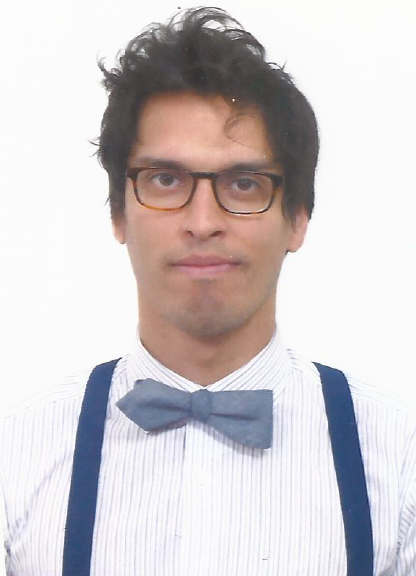
\includegraphics[width=0.2\textwidth]{1-introduction/img/georges-louis-joseph-labreche.jpg}  & \textbf{Georges L. J. Labrèche - Management Division}

\smallskip
\textit{Current Education}: MSc in Spacecraft Design.

\smallskip
\textit{Previous Education}: BSc in Software Engineering with experience in technical leadership and project management in software development.

\smallskip
\textit{Responsibilities}: Acting as Systems Engineer / Project Manager and managing overall implementation of the project until the Critical Design Review (CDR). Establishing and overseeing product development cycle. Coordinating between different teams, project stakeholders, and documentation efforts.                          
\bigskip
\\

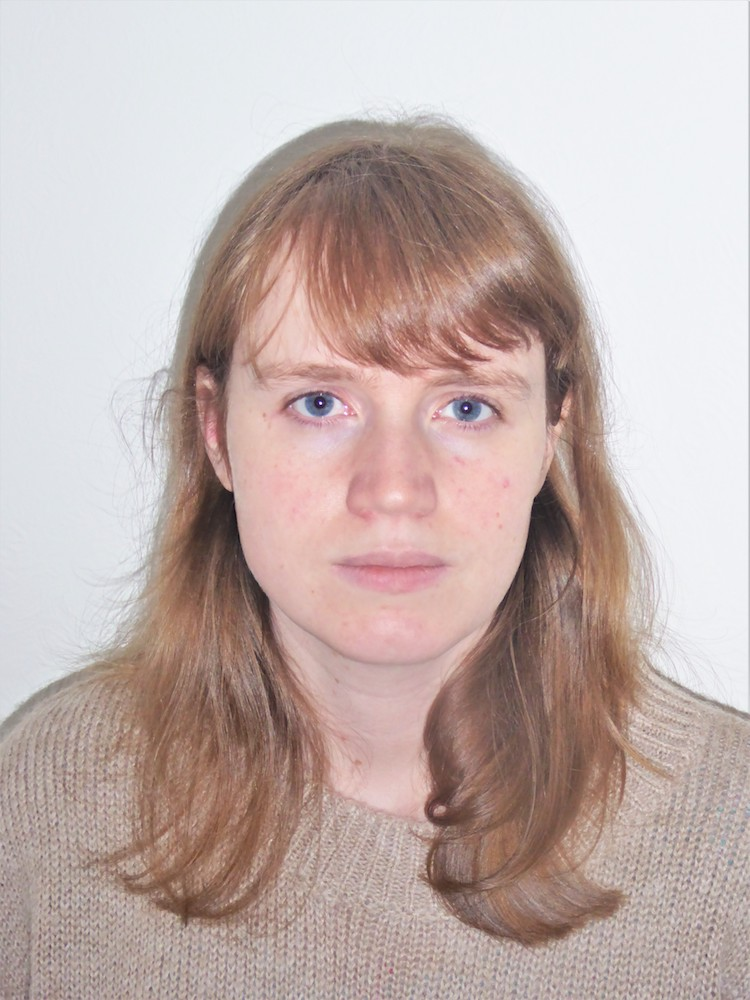
\includegraphics[width=0.2\textwidth]{1-introduction/img/natalie-lawton.jpg} & \textbf{Natalie Lawton - Management and Electrical Division}

\smallskip
\textit{Current Education}: MSc in Spacecraft Design.

\smallskip
\textit{Previous Education}: MEng in Aerospace Engineering. Previous experience in UAV avionic systems and emissions measurement techniques.

\smallskip
\textit{Responsibilities}: Acting as Deputy Systems Engineer / Project Manager until the CDR. Assuming role of System Engineer / Project Manager after the CDR until end of project. Supporting designing and implementing cost-effective circuitry using analysis and computer-aided design; Reviewing and testing proposed designs; recommending modifications following prototype test results; assembling designed circuitry. 
\bigskip
\\

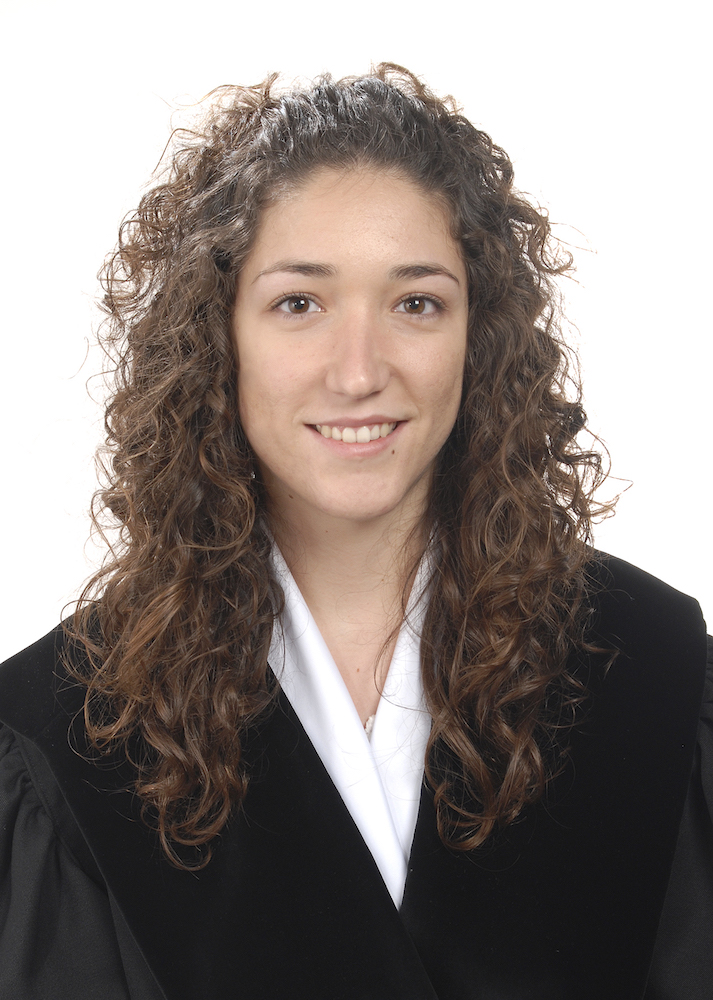
\includegraphics[width=0.2\textwidth]{1-introduction/img/agues-paszkowsky.jpg} & \textbf{Nuria Agües Paszkowsky - Scientific Division}

\smallskip
\textit{Current Education}: MSc in Earth Atmosphere and the Solar System.

\smallskip
\textit{Previous Education}: BSc in Aerospace Engineering.

\smallskip
\textit{Responsibilities}: Defining experiment parameters; data analysis; interpreting and documenting measurements; research on previous CAC experiments for comparative analysis purposes; contacting researchers or institutions working on similar projects; exploring potential partnership with researchers and institutions, evaluating the reliability of the proposed AAC sampling system; conducting measurements of collected samples; documenting and publishing findings. 
\bigskip
\\

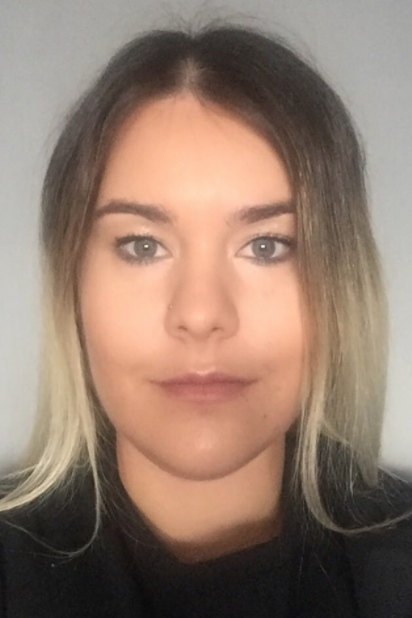
\includegraphics[width=0.2\textwidth]{1-introduction/img/kiki-blazaki.jpg} & \textbf{Kyriaki Blazaki - Scientific Division}

\smallskip
\textit{Current Education}: MSc in Earth Atmosphere and the Solar System.

\smallskip
\textit{Previous Education}: BSc in Physics.


\smallskip
\textit{Responsibilities}: Coordinating between the Scientific Division and the Project Manager; defining experiment parameters; data analysis; interpreting and documenting measurements; research on previous CAC experiments for comparative analysis purposes; evaluating the reliability of the proposed AAC sampling system; conducting measurements of collected samples; documenting and publishing findings. 
\bigskip
\\

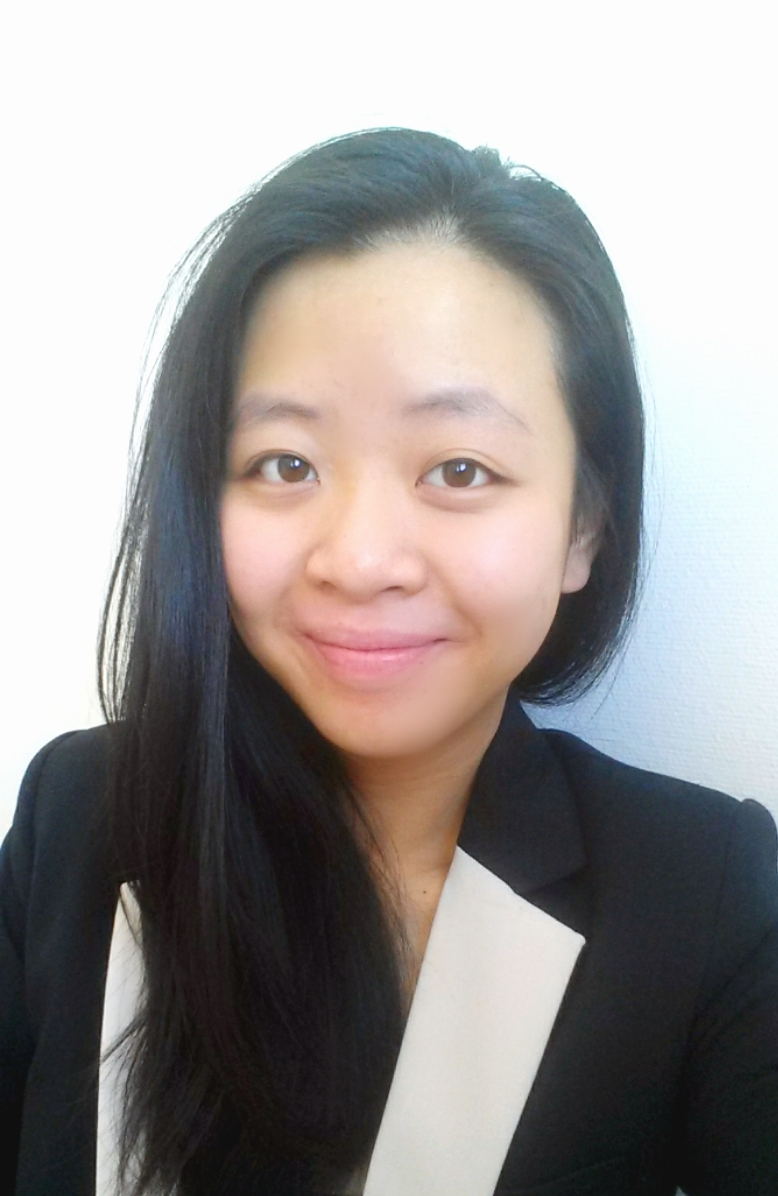
\includegraphics[width=0.2\textwidth]{1-introduction/img/emily-chen.jpeg} & \textbf{Emily Chen - Mechanical Division}

\smallskip
\textit{Current Education}: MSc in Space Engineering (4th Year).


\smallskip
\textit{Responsibilities}: Mechanical designing and assembly of CAC subsystem; analyzing the test results and changing the design as needed in collaboration with the team leader; integrating and assembling final design. 
\bigskip
\\

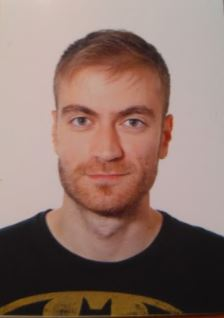
\includegraphics[width=0.2\textwidth]{1-introduction/img/jordi-coll-ortega.jpg} & \textbf{Jordi Coll Ortega - Mechanical Division}

\smallskip
\textit{Current Education}: MSc in Spacecraft Design.

\smallskip
\textit{Previous Education}: BASc in Aerospace Vehicle Engineering.

\smallskip
\textit{Responsibilities}: Designing or redesigning cost-effective mechanical devices using analysis and computer-aided design; developing and testing prototypes of designed devices; analyzing the test results and changing the design as needed in collaboration with the team lead; integrating and assembling final design.
\bigskip
\\

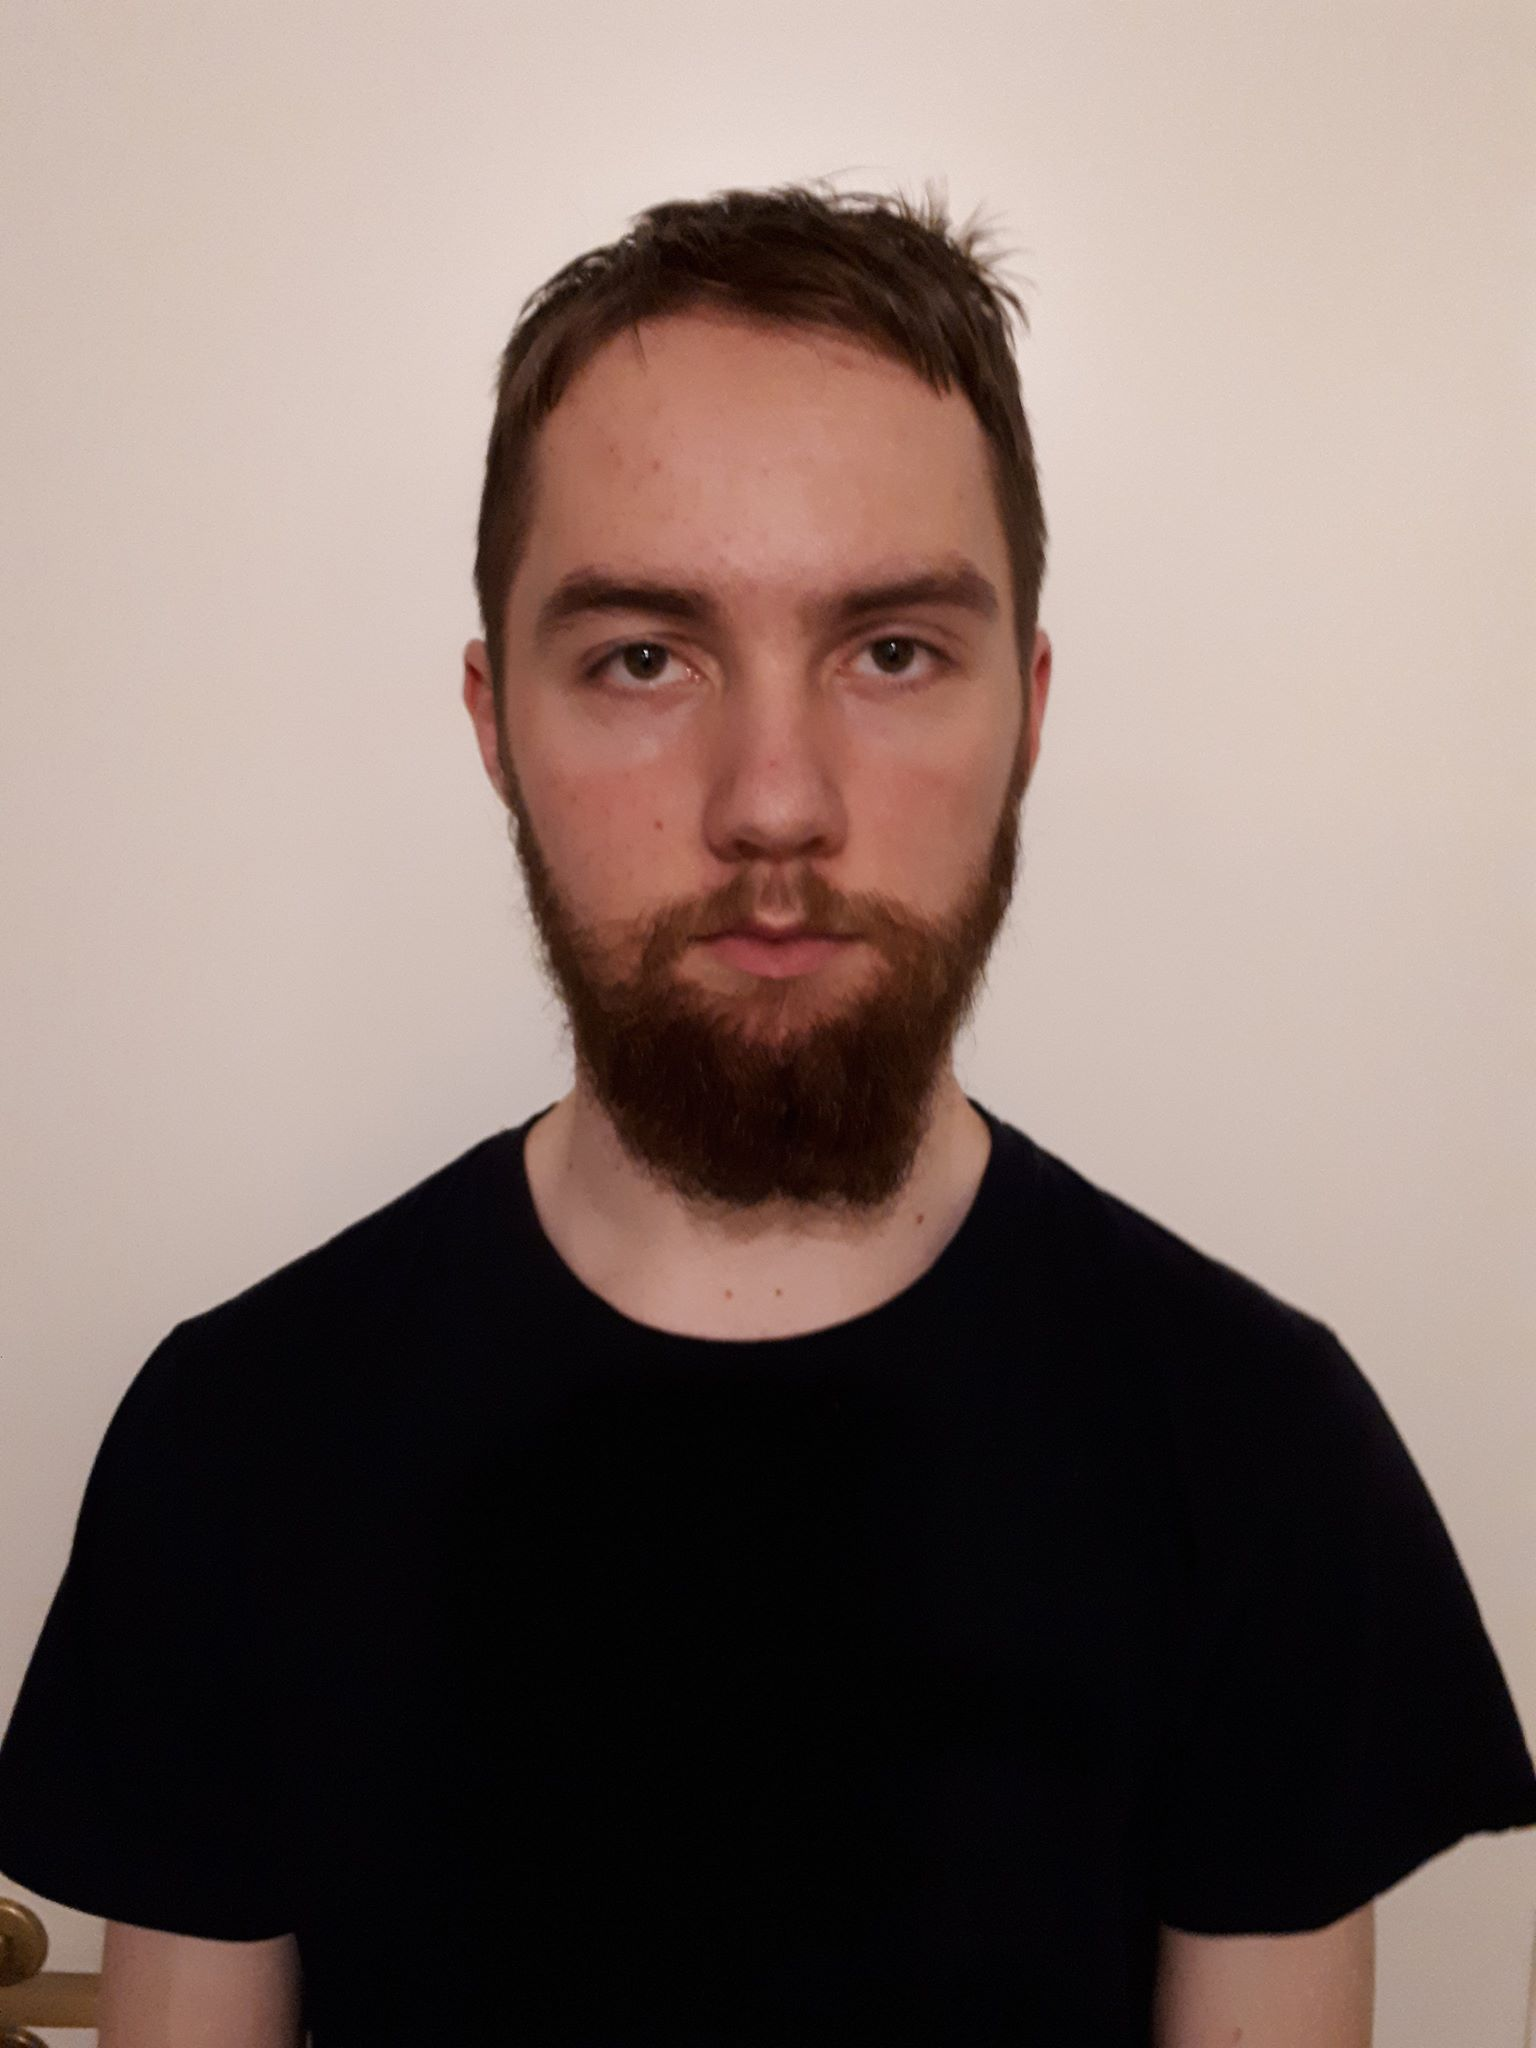
\includegraphics[width=0.2\textwidth]{1-introduction/img/gustav-dryssen.jpg} & \textbf{Gustav Dyrssen - Software Division}

\smallskip
\textit{Current Education}: MSc in Space Engineering (4th Year).

\smallskip
\textit{Responsibilities}: Leading quality assurance and testing efforts; Enforcing software testing best practices such as continuous integration testing and regression testing; reviewing requirements and specifications in order to foresee potential issues; provide input of functional requirements; advising on design; formalizing test cases; tracking defects and ensuring their resolution; facilitating code review sessions; supporting software implementation efforts.     
\bigskip
\\



\includegraphics[width=0.2\textwidth]{1-introduction/img/erik-fagerstrom.jpg} & \textbf{Erik Fagerström - Thermal Division}

\smallskip
\textit{Current Education}: MSc in Space Engineering (4th Year).


\smallskip
\textit{Responsibilities}: Coordinating between the Thermal Division and the Project Manager. Planning project thermal analysis and testing strategy. Thermal simulations of proposed designs and analyze results.
\bigskip
\\


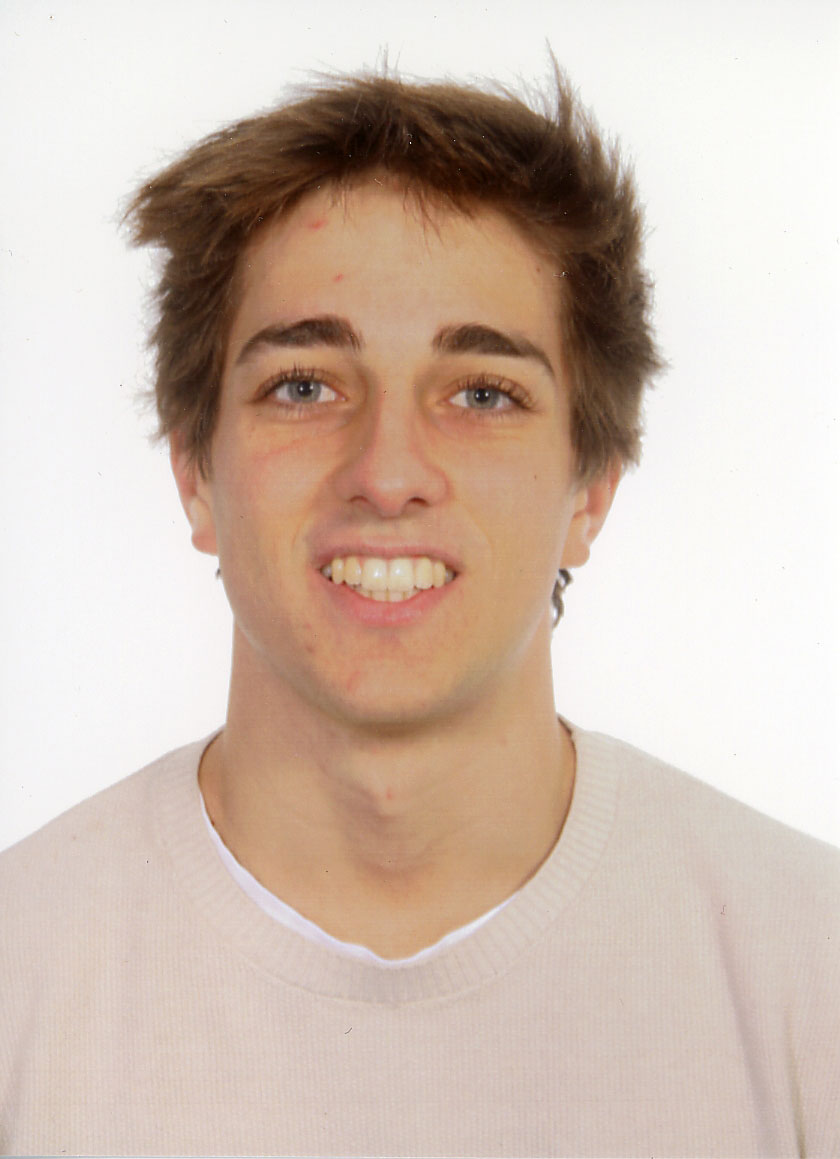
\includegraphics[width=0.2\textwidth]{1-introduction/img/pau-molas-roca.jpg} & \textbf{Pau Molas Roca - Mechanical Division}

\smallskip
\textit{Current Education}: MSc in Spacecraft Design.

\smallskip
\textit{Previous Education}: BSc in Aerospace Technology Engineering, Mechanical experience.

\smallskip
\textit{Responsibilities}: Coordinating between the Mechanical Division and the Project Manager; designing or redesigning cost-effective mechanical devices using analysis and computer-aided design; producing details of specifications and outline designs; overseeing the manufacturing process for the devices; identifying material and component suppliers; integrating and assembling final design.   \bigskip
\\


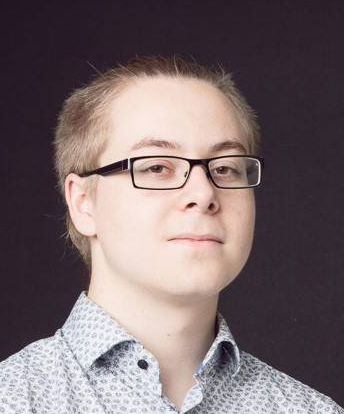
\includegraphics[width=0.2\textwidth]{1-introduction/img/emil-nordqvist.jpg} & \textbf{Emil Nordqvist - Electrical Division}

\smallskip
\textit{Current Education}: MSc in Space Engineering (4th Year).

\smallskip
\textit{Responsibilities}: Quality assurance of circuit design and implementation. Developing, testing, and evaluating theoretical designs.  \bigskip
\\

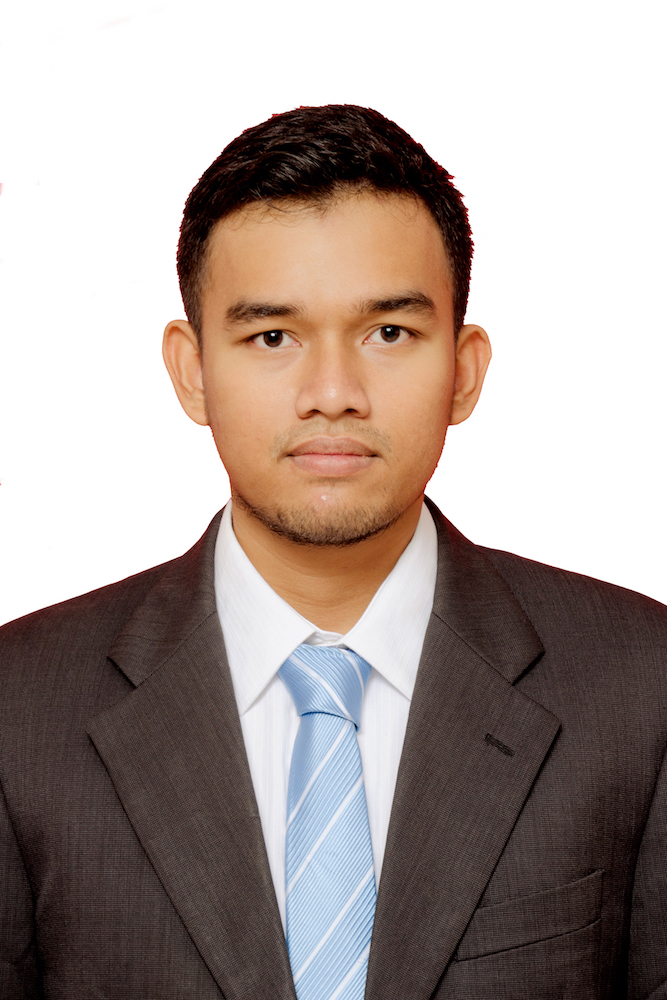
\includegraphics[width=0.2\textwidth]{1-introduction/img/muhammad-ansyar-rafi-putra.jpg} & \textbf{Muhammad Ansyar Rafi Putra - Software Division}

\smallskip
\textit{Current Education}: MSc in Spacecraft Design.

\smallskip
\textit{Previous Education}: BSc in Aerospace Engineering.


\smallskip 
\textit{Responsibilities}: Coordinating between the Software Division and the Project Manager; gathering software requirements; formalizing software specifications; drafting architecture design, detailed design; leading software implementation efforts.
\bigskip
\\

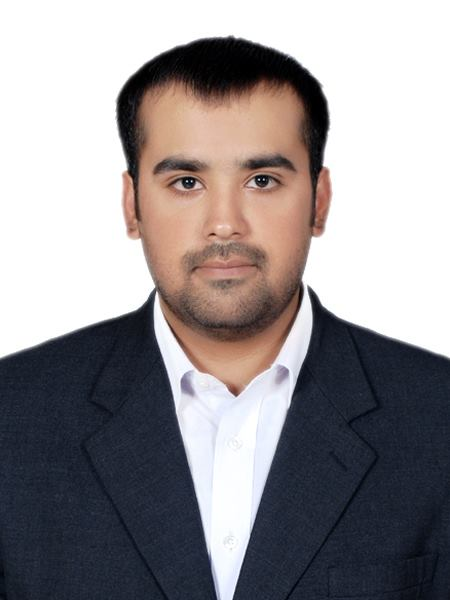
\includegraphics[width=0.2\textwidth]{1-introduction/img/hamad-saddiqi.jpg} & \textbf{Hamad Siddiqi - Electrical Division}


\smallskip
\textit{Current Education}: MSc Satellite Engineering.

\smallskip
\textit{Previous Education}: BSc in Electrical Engineering with experience in telecommunication industry and electronics.

\smallskip
\textit{Responsibilities}: Coordinating between the Electrical Division and the Project Manager; designing and implementing cost-effective circuitry using analysis and computer-aided design; producing details of specifications and outline designs; developing, testing, and evaluating theoretical designs; identifying material as well as component suppliers. 
\bigskip
\\


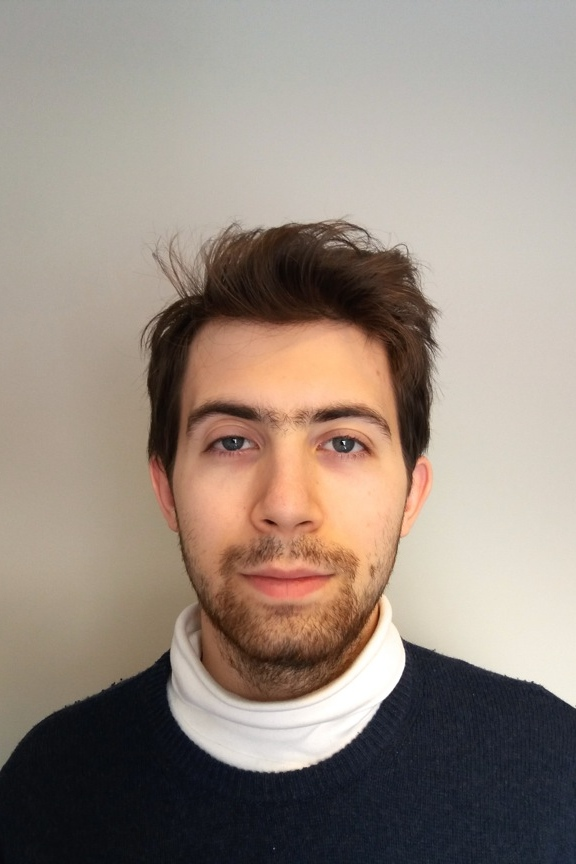
\includegraphics[width=0.2\textwidth]{1-introduction/img/ivan-zankov.jpg} & \textbf{Ivan Zankov - Thermal Division}

\smallskip
\textit{Current Education}: MSc in Spacecraft Design.

\smallskip
\textit{Previous Education}: BEng in Mechanical Engineering.

\smallskip
\textit{Responsibilities}: Thermal analysis of proposed designs and analysis result based recommendations.                                                         

\\
\label{tab:people}
\end{longtable}
\raggedbottom

\pagebreak
\section{Experiment Requirements and Constraints}
Requirements in this section does not list obsolete requirements. For a complete list of requirements that include obsolete ones, refer to Appendix \ref{sec:appFullListOfRequirements}.

\subsection{Functional Requirements}

\begin{enumerate}
    \item[F.2] The experiment \textit{shall} collect air samples by the CAC.
    \item[F.3] The experiment \textit{shall} collect air samples by the AAC.
    \item[F.9] The experiment \textit{should} measure the air intake flow to the AAC.
    \item[F.10] The experiment \textit{shall} measure the air pressure.
    \item[F.11] The experiment \textit{shall} measure the temperature.
\end{enumerate}
\subsection{Performance Requirements}

\begin{enumerate}
    %\item The programmable sampling rate of the pressure sensor \textit{shall} not be lesser than .
    \item[P.12] The accuracy of the ambient pressure measurements \textit{shall} be -1.5/+1.5 mbar for 25$\degree$C.
    \item[P.13] The accuracy of temperature measurements \textit{shall} be +3.5/-3$\degree$C (max) for condition of -55$\degree$C to 150$\degree$C.
    \item[P.23] The temperature sensor sampling rate \textit{shall} be 1 Hz.\label{newsamplerate}
    \item[P.24] The temperature of the Pump \textit{shall} be between 5$\degree$C and 40$\degree$C. 
    \item[P.25] The minimum volume of air in the bags for analysis \textit{shall} be 0.18 L at ground level.
    \item[P.26] The flow rate of the pump \textit{shall} be between 8 to 3 L/min from ground level up to 24 km altitude.
    \item[P.27] The accuracy range of the sampling time, or the resolution, \textit{shall} be less than 52.94 s, or 423.53 m.
    \item[P.28] The pressure sensor sampling rate \textit{shall} be 1 Hz.\label{newsamplerate}
    \item[P.29] The airflow sensor sampling rate \textit{shall} be 1 Hz.\label{newsamplerate}
    \item[P.30] The accuracy of the pressure measurements inside the tubing and sampling bags \textit{shall} be -0.005/+0.005 bar for 25$\degree$C.

 \end{enumerate} 
\pagebreak
\subsection{Design Requirements}

\begin{enumerate}
    \item[D.1] The experiment \textit{shall} operate in the temperature profile of the BEXUS flight\cite{BexusManual}.
    \item[D.2] The experiment \textit{shall} operate in the vibration profile of the BEXUS flight\cite{BexusManual}.
    \item[D.3] The experiment \textit{shall} not have sharp edges or loose connections to the gondola that can harm the launch vehicle, other experiments, and people.%\textsuperscript{\ref{fn:unnecessary-requirement}}
    \item[D.4] The experiment's communication system \textit{shall} be compatible with the gondola's E-link system with the RJF21B connector over UDP for down-link and TCP for up-link.
    \item[D.5] The experiment's power supply \textit{shall} have a 24v, 12v, 5v and 3.3v power output and be able to take 28.8v input through the Amphenol PT02E8-4P connector supplied from the gondola. 
    \item[D.7] For the supplied voltage of 28.8 V, the total continuous DC current draw \textit{should} be below 1.8 A.
    \item[D.8] The total power consumption \textit{should} be below 374 Wh.
    \item[D.16] The experiment \textit{shall} be able to autonomously turn itself off just before landing.
    \item[D.17] The experiment box \textit{shall} be placed with at least one face exposed to the outside.
    \item[D.18] The experiment \textit{shall} operate in the pressure profile of the BEXUS flight\cite{BexusManual}.
    \item[D.19] The experiment \textit{shall} operate in the vertical and horizontal accelerations profile of the BEXUS flight\cite{BexusManual}.
    \item[D.21] The experiment \textit{shall} be attached to the gondola's rails.
    \item[D.22] The telecommand data rate \textit{shall} not be over 10 kb/s.
    \item[D.23] The air intake rate of the air pump \textit{shall} be minimum 3 L/min at 24 km altitude.
    \item[D.24] The temperature of the Brain\DIFaddbegin \footnote{\DIFadd{The Brain is a central command unit which contains Electronic Box and pneumatic sampling system.}} \DIFaddend \textit{shall} be between -10$\degree$C and 25$\degree$C.
    \item[D.26] The air sampling systems \textit{shall} filter out all water molecules before filling the sampling bags.
    \item[D.27] The total weight of the experiment \textit{shall} be less than 28 kg.
    \item[D.28] The AAC box \textit{shall} be able to fit at least $6$ air sampling bags.
    \item[D.29] The CAC box \textit{shall} take less than 3 minutes to be removed from the gondola without removing the whole experiment.
    \item[D.30] The AAC \textit{shall} be re-usable for future balloon flights.
    \item[D.31] The altitude from which a sampling bag will start sampling \textit{shall} be programmable.
    \item[D.32] The altitude from which a sampling bag will stop sampling \textit{shall} be programmable.
\end{enumerate}
\pagebreak
\pagebreak
\subsection{Operational Requirements}

\begin{enumerate}
    \item[O.13] The experiment \textit{should} function automatically.
    \item[O.14] The experiment's air sampling mechanisms \textit{shall} have a manual override.
\end{enumerate} 
\subsection{Constraints}

\begin{enumerate}
    \item[C.1] Constraints specified in the BEXUS User Manual.
\end{enumerate}



\pagebreak
\section{Project Planning}

\subsection{Work Breakdown Structure}

The team is categorized into different groups of responsibilities with dedicated leaders who will report to and coordinate with the Project Manager. Leadership may be organized on a rotational basis should the need arise. The formation of these divisions constitute a work breakdown structure in which is illustrated in Figure \ref{fig:work-breakdown-structure}.


The interaction between the divisions will be refined over the course of project implementation to acknowledge the interdisciplinary nature of the experiment around a Payload / Platform scheme.

The Management is composed of a Project Manager and a Deputy Project Manager, both acting as Systems Engineer and managing overall implementation of the project. The Project Manager is responsible for establishing and overseeing product development cycle; coordinating between different teams, project stakeholders, and documentation efforts; outreach and public relations; Fundraising; monitoring and reporting; system integration; and quality assurance. Once all subsystems have been assembled, the Project Manager will be responsible for overseeing the integration processes leading to the final experiment setup and will put emphasis on leading quality assurance integration testing efforts. The Deputy Project Manager assists the Project Manager in all management duties in a manner that ensures replaceability when necessary.

The Scientific Division is responsible for defining experiment parameters; data analysis; interpreting and documenting measurements; researching previous CAC experiments for comparative analysis purposes; evaluating the reliability of the proposed AAC sampling system; conducting measurements of collected samples; documenting and publishing findings; defining experiment parameters; contacting researchers or institutions working on similar projects; exploring potential partnership with researchers and institutions; documenting and publishing findings.

The Mechanical Division is responsible for designing or redesigning cost-effective mechanical devices using analysis and computer-aided design; producing details of specifications and outline designs; overseeing the manufacturing process for the devices; identifying material and component suppliers; developing and testing prototypes of designed devices; analyzing test results and changing the design as needed; and integrating and assembling final design.

The Electrical Division is responsible for designing and implementing cost-effective circuitry using analysis and computer-aided design; producing details of specifications and outline designs; developing, testing, and evaluating theoretical designs; identifying material as well as component suppliers; reviewing and testing proposed designs; recommending modifications following prototype test results; and assembling designed circuitry.

The Software Division is responsible for gathering software requirements; formalizing software specifications; drafting architecture design; leading software implementation efforts; leading quality assurance and testing efforts; enforcing software testing best practices such as continuous integration testing and regression testing; reviewing requirements and specifications in order to foresee potential issues; providing input for functional requirements; advising on design; formalizing test cases; tracking defects and ensuring their resolution; facilitating code review sessions; and supporting software implementation efforts.

The Thermal Division is responsible for ensuring thermal regulation of the payload as per operational requirements of all experiment components; evaluating designs against thermal simulation and propose improvements; managing against mechanical design and electrical power limitations towards providing passive and active thermal control systems.

\begin{landscape}
\begin{figure}[p]
    \begin{align*}
        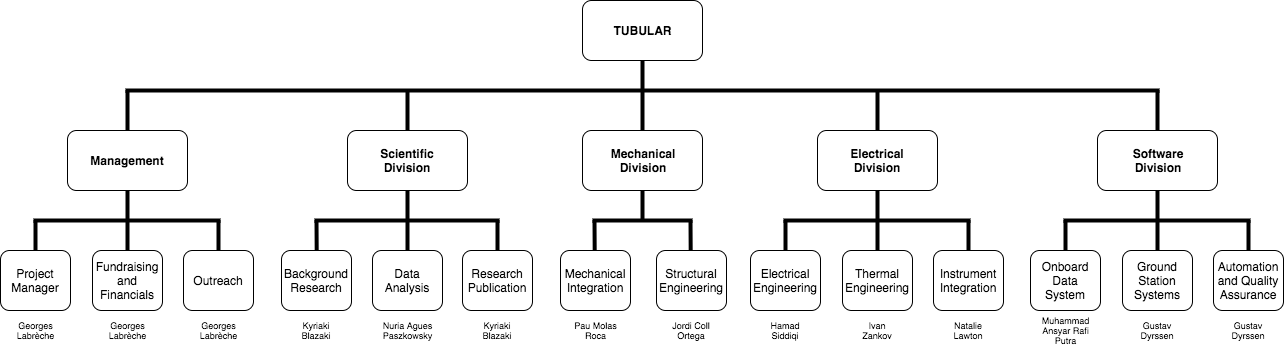
\includegraphics[width=24cm]{3-project-planning/img/work-breakdown-structure.png}
    \end{align*}
    \caption{Work Breakdown Structure.}\label{fig:work-breakdown-structure}
\end{figure}
\end{landscape}
\pagebreak
\subsection{Schedule}

Scheduling of the project is presented in a Gantt Chart overview on Figure \ref{fig:schedule-gantt-chart}. Exam period constraints have been included in order to evaluate risks in person-day allocations to project implementation. It is expected during exam periods the team work output will be lower than usual but project activities will continue, therefore time has been planned accordingly to accommodate this:

\begin{figure}[H]
    \begin{align*}
        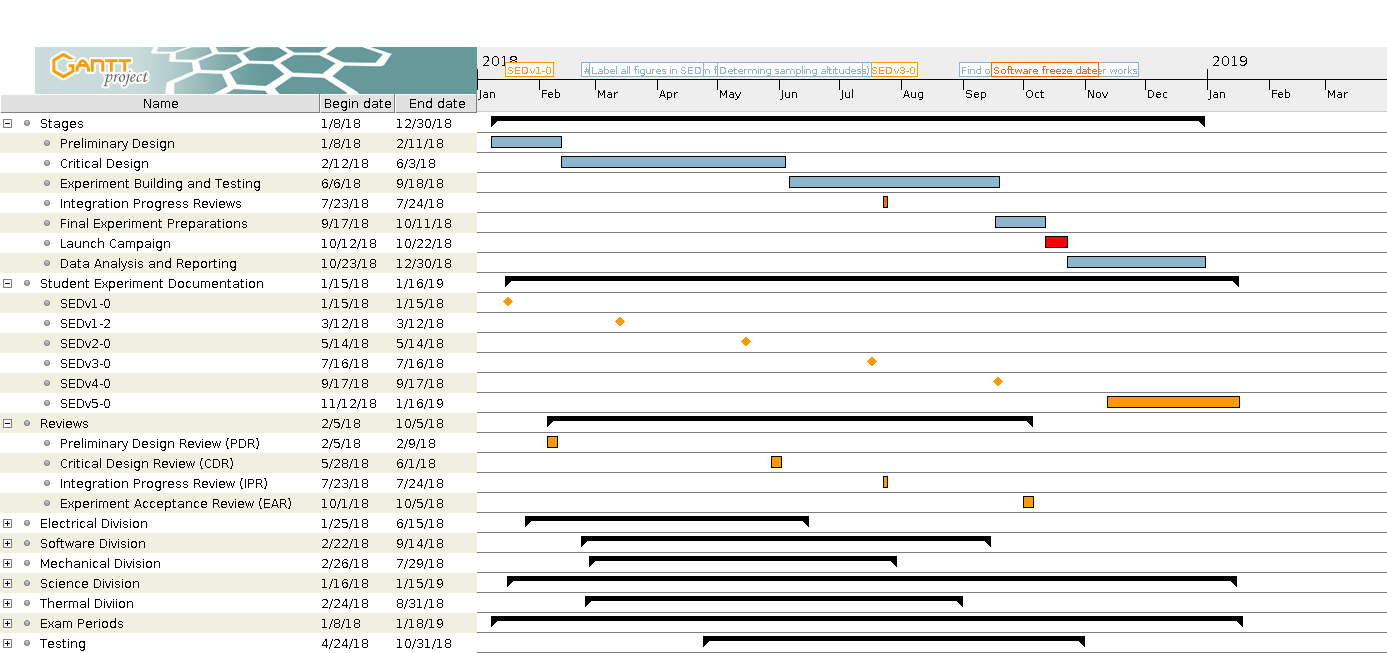
\includegraphics[width=1\linewidth]{3-project-planning/img/BEXUS-SED-GanttChart-Overview.png}
    \end{align*}
    \caption{Project Schedule Gantt Chart.}\label{fig:schedule-gantt-chart}
\end{figure}

Deadlines of the five Student Experiment Documentations (SED) versions have been estimated based on past REXUS/BEXUS Cycles. An expanded version of the Gantt Chart with detailed listing of all sub-tasks not shown in Figure \ref{fig:schedule-gantt-chart} can be found in Appendix \ref{sec:appF}. This expanded Gantt Chart includes all tasks related to the test plan and internal deadlines are set so that a first draft of the documentation is completed one week in advance to allow contents to be checked. Build and test internal deadlines are also placed one week in advance to allow a buffer in case things do not go as expected. The tests are scheduled for as early as possible to allow time for rescheduling if the result is a fail. With some high priority tests, see Section \ref{sec:5.2.1-testpriority}, it is expected these will be very difficult to reschedule therefore extra time is built into the test duration to allow for multiple attempts at the test.


\pagebreak
\subsection{Resources}

\subsubsection{Manpower}
The TUBULAR Team is categorized into divisions as summarized in Table \ref{tab:divisions-members}:

\begin{table}[H]
\centering
\DIFdelbeginFL %DIFDELCMD < \resizebox{\textwidth}{!}{%
%DIFDELCMD < \begin{tabular}{|l|l|l|l|l|l|}
%DIFDELCMD < \hline
%DIFDELCMD < \textbf{Management} & \textbf{Scientific}    & \textbf{Mechanical} & \textbf{Electrical} & \textbf{Thermal} & \textbf{Software}          \\ \hline
%DIFDELCMD < Georges L. J. Labrèche*    & Kyriaki Blazaki*        & Pau Molas Roca*      & Hamad Siddiqi*  & Erik Fragerström*    & Muhammad Ansyar Rafi Putra* \\ \hline
%DIFDELCMD < Natalie Lawton & Nuria Agues Paszkowsky & Jordi Coll Ortega   & Natalie Lawton  & Ivan Zankov  & Gustav Dyrssen             \\ \hline
%DIFDELCMD <  & & Emily Chen  & Emil Nordqvist  &  &              \\ \hline
%DIFDELCMD < \end{tabular}%
%DIFDELCMD < }
%DIFDELCMD < %%%
\DIFdelendFL \DIFaddbeginFL \resizebox{\textwidth}{!}{%
\begin{tabular}{|l|l|l|l|l|l|}
\hline
\textbf{Management} & \textbf{Scientific}    & \textbf{Mechanical} & \textbf{Electrical} & \textbf{Thermal} & \textbf{Software}          \\ \hline
Natalie Lawton*    & Kyriaki Blazaki*        & Pau Molas Roca*      & Hamad Siddiqi*  & Erik Fragerström*    & Muhammad Ansyar Rafi Putra* \\ \hline
Georges L. J. Labrèche & Nuria Agues Paszkowsky & Jordi Coll Ortega   & Natalie Lawton  & Ivan Zankov  & Gustav Dyrssen             \\ \hline
 & & Emily Chen  & Emil Nordqvist  &  &              \\ \hline
\end{tabular}%
}
\DIFaddendFL \caption{Project Divisions and Members (Asterisks Denote Division Leaders).}
\label{tab:divisions-members}
\end{table}
\raggedbottom

The experience of TUBULAR Team members are listed in Table \ref{tab:team-member-experience}:

% Please add the following required packages to your document preamble:
% \usepackage{graphicx}
\begin{table}[H]
\centering
\begin{tabular}{|l|m{11cm}|}
\hline
\textbf{Team Member} & \textbf{Project Related Experience} \\ \hline
Georges L. J. Labrèche & MSc in Spacecraft Design (2nd Year). \\& BSc in Software Engineering.\\ \hline
Nuria Agues Paszkowsky & MSc in Earth Atmosphere and the Solar System (2nd Year). \\& BSc in Aerospace Engineering.\\ \hline
Kyriaki Blazaki & MSc in Earth Atmosphere and the Solar System (2nd Year). \\& BSc in Physics. \\ \hline
Emily Chen & MSc in Space Engineering (4th Year). \\ \hline
Jordi Coll Ortega & MSc in Spacecraft Design (2nd Year). \\& BSc in Aerospace Vehicle Engineering. \\ \hline
Gustav Dyrssen &  MSc in Space Engineering (4th Year).\\ \hline
Erik Fagerström & MSc in Space Engineering (4th Year). \\ \hline
Natalie Lawton & MSc in Spacecraft Design (2nd Year). \\& MEng in Aerospace Engineering.\\& Previous experience in UAV avionic systems and emissions measurement techniques. \\ \hline
Muhammad Ansyar Rafi Putra & MSc in Spacecraft Design (2nd Year). \\& BSc in Aerospace Engineering. \\ \hline
Pau Molas Roca & BSc in MSc in Spacecraft Design (2nd Year). \\& Aerospace Technology Engineering, Mechanical experience. \\ \hline
Emil Nordqvist & MSc in Space Engineering (4th Year). \\ \hline
Hamad Siddiqi & MSc Satellite Engineering (4th Year) \\&  BSc in Electrical Engineering.\\& Experience in telecommunication industry and electronics.  \\ \hline
Ivan Zankov & MSc in Spacecraft Design (2nd Year). \\& BEng in Mechanical Engineering.\\ \hline
\end{tabular}
\caption{Project Related Experience of Team Members.}
\label{tab:team-member-experience}
\end{table}
\raggedbottom

The initial projected effort to be contributed by each team member was averaged at 1.5 hour per person per day corresponding to a team total of 15 hours per day. Since then, 3 new members have been included in the team thus increasing the projected daily effort to 19.5 hours per day. During the period leading up to the launch it is expected that the effort contributed will be double to 3 hours per person per day. The period of these different effort capacities are listed in Table \ref{tab:daily-team-effort-per-period}:

\begin{table}[H]
\centering
\begin{tabular}{|c|c|c|}
\hline
\textbf{From} & \textbf{To} & \textbf{Capacity (hours/day)} \\ \hline
08/01/2018 & 18/03/2018 & 15 \\ \hline
19/03/2018 & 08/04/2018 & 16.5 \\ \hline
09/04/2018 & 09/05/2018 & 18 \\ \hline
10/05/2018 & 15/08/2018 & 19.5 \\ \hline
15/08/2018 & 22/10/2018 & 39 \\ \hline
23/10/2018 & 31/01/2019 & 19.5 \\ \hline
\end{tabular}
\caption{Projected Daily Team Effort per Period.}
\label{tab:daily-team-effort-per-period}
\end{table}

Taking into account all team members and the mid-project changes in team size, the efforts/capacity projected to be allocated to each stages of the project during 2018 are summarized in Table \ref{tab:effort-allocation-stages}:

\begin{table}[H]
\centering
\begin{tabular}{lcc|c|c|c|c|}
\hline
\multicolumn{1}{|c|}{\multirow{2}{*}{\textbf{Stage}}} & \multicolumn{1}{c|}{\multirow{2}{*}{\textbf{\begin{tabular}[c]{@{}c@{}}Start\\ Date\end{tabular}}}} & \multirow{2}{*}{\textbf{\begin{tabular}[c]{@{}c@{}}End\\ Date\end{tabular}}} & \multirow{2}{*}{\textbf{\begin{tabular}[c]{@{}c@{}}Duration\\ (days)\end{tabular}}} & \multicolumn{3}{c|}{\textbf{Effort (hours)}} \\ \cline{5-7} 
\multicolumn{1}{|c|}{} & \multicolumn{1}{c|}{} &  &  & \textbf{Capacity} & \textbf{Actual} & \multicolumn{1}{l|}{\textbf{Diff. (\%)}} \\ \hline
\multicolumn{1}{|l|}{Preliminary Design} & \multicolumn{1}{c|}{08/01} & 11/02 & 35 & 525 & 708 & +29.68 \\ \hline
\multicolumn{1}{|l|}{Critical Design} & \multicolumn{1}{c|}{12/02} & 03/06 & 112 & 1680 & \textit{2299} & \textit{+36.9} \\ \hline
\multicolumn{1}{|l|}{Experiment Building and Testing} & \multicolumn{1}{c|}{04/06} & 16/09 & 105 & 3072 & \DIFdelbeginFL \DIFdelFL{720* }\DIFdelendFL \DIFaddbeginFL \DIFaddFL{798* }\DIFaddendFL & \DIFdelbeginFL \DIFdelFL{-76.56 }\DIFdelendFL \DIFaddbeginFL \DIFaddFL{-74.01* }\DIFaddendFL \\ \hline
\multicolumn{1}{|l|}{Final Experiment Preparations} & \multicolumn{1}{c|}{17/09} & 11/10 & 25 & 976 & - & - \\ \hline
\multicolumn{1}{|l|}{Launch Campaign} & \multicolumn{1}{c|}{12/10} & 22/10 & 10 & 390 & - & - \\ \hline
\multicolumn{1}{|l|}{Data Analysis and Reporting} & \multicolumn{1}{c|}{23/10} & 30/12 & 69 & 1346 & - & - \\ \hline
\multicolumn{1}{r}{\textbf{}} & \multicolumn{1}{l}{} & \multicolumn{1}{r|}{\textbf{Total:}} & \textbf{353} & \textbf{6282} & \textit{3727*} & \textit{-40.67*} \\ \cline{4-7} 
\end{tabular}
\caption{Project Effort Allocation per Project Stages (Asterisks Denote Still Ongoing Stages).}
\label{tab:effort-allocation-stages}
\end{table}

All TUBULAR Team members are based in Kiruna, Sweden, just 40 kilometers from Esrange Space Center. Furthermore, all team members are enrolled in LTU Master programmes in Kiruna and thus expected to remain in LTU during the entire project period. Special attention will have to be made for planning tasks during the summer period where many team members are expected to travel abroad. A timeline of team member availability  until January 2019 is available in Appendix \ref{sec:appD}. A significant risk can be observed during the summer months from June to August where most members will only be partially available and some completely unavailable. As such, team member availability and work commitments over the summer have been negotiated across team members in order to guarantee that at least one member per division is present in Kiruna over the Summer with the exception of the Software Division which can work remotely. Furthermore, the Project Manager role will have to be assigned to the Deputy Project Manager due to an extended full time unavailability after the CDR.

As part of their respective Master programmes, most TUBULAR Team members are enrolled in a project course at LTU. The TUBULAR project acts as the course's project for most team members from which they will obtain ECTS credits. This course is supervised by Dr. Thomas Kuhn, Associate Professor at LTU.

\pagebreak
\subsubsection{Budget}
\label{sec:3.2.2}
The project mass and cost budget is summarized in Table \ref{table:mass-and-cost-budget} for a total project mass of 24 Kg and cost of 31,228 EUR. A complete budget is available in Appendix \ref{sec:appO} and a detailed component mass and cost breakdown is available in Section \ref{sec:experiment-components} Experiment Components. The component mass and cost breakdown does not include spare components accounted for in the total costs listed in Table \ref{table:mass-and-cost-budget}. A contingency fund of 1,054 EUR is allocated for unseen events such as component failures. Furthermore, an error margin is included in the budget corresponding to 10\% of the total costs of components to be purchased. Component loan and donations from sponsors account for 83\% of the project's total cost. LTU and SNSB funding accounts for the remaining 17\%. 


\begin{table}[H]
\centering
\begin{tabular}{|c|d{2}|d{2}|}%{D{.}{.}{1}}
\hline

\textbf{Category} & \textbf{Total Mass [g]} & \textbf{Total Price [EUR]} \\ \hline
Structure & \color{blue}{11,337.84} & \color{blue}{619.24} \\ \hline
Electronics Box & \color{blue}{510.50} & \color{blue}{1062.74} \\ \hline
Cables and Sensors & \color{blue}{1,200.62} & \color{blue}{586.20} \\ \hline
CAC & 5,539.00 & 23,114.00 \\ \hline
AAC & 3,541.00 & 4,444.71 \\ \hline
Tools & - & \color{blue}{332.53} \\ \hline
Travel & - & 500.00 \\ \hline
Contingency & - & \color{blue}{1053.86} \\ \hline
Shipping Costs and Error Margin & \color{blue}{2,212.90} & \color{blue}{568.17} \\ \hline
{\textbf{Total}} & \color{blue}{\textbf{24,341.85}} & \color{blue}{\textbf{31,227.58}} \\ \hline
\end{tabular}
\caption{Mass and Cost Budget.}
\label{table:mass-and-cost-budget}
\end{table}

\raggedbottom

The project benefits from component donations from Restek, SMC Pneumatics, Teknolab Sorbent, and Lagers Masking Consulting as well as component loans from FMI. Furthermore, discounts were offered by Teknolab Sorbent and Bosch Rexroth. Euro value allocation of these sponsorships are presented in Table \ref{table:sponsroship-allocation}.

\begin{table}[H]
\centering
\begin{tabular}{l|m{0.12\textwidth}|l|r|r|r|c}
\hline
\multicolumn{1}{|l|}{\textbf{Sponsor}} & \multicolumn{1}{|c|}{\textbf{Type}} & \multicolumn{1}{c|}{\textbf{Value}} & \multicolumn{1}{c|}{\textbf{Allocated}} & \multicolumn{1}{c|}{\textbf{Unallocated}} & \multicolumn{1}{c|}{\textbf{\% Allocation}} & \multicolumn{1}{c|}{\textbf{Status}} \\ \hline
\multicolumn{1}{|l|}{LTU} & Funds & 2,500.00 & \color{blue}{1,880.33} & \color{blue}{619.67} & \color{blue}{75} & \multicolumn{1}{c|}{Received} \\ \hline
\multicolumn{1}{|l|}{SNSB} & Funds & 2,909.80 & \color{blue}{2,475.60} & \color{blue}{434.20} & \color{blue}{85} & \multicolumn{1}{c|}{Received} \\ \hline
\multicolumn{1}{|l|}{FMI} & Component loan & \color{blue}{22,500.00} & \color{blue}{22,500.00} & 0.00 & 100 & \multicolumn{1}{c|}{Confirmed} \\ \hline
\multicolumn{1}{|l|}{Restek} & Component donation & \color{blue}{1040.00} & \color{blue}{1040.00} & \color{blue}{0.00} & \color{blue}{} & \multicolumn{1}{c|}{\color{blue}{Received}} \\ \hline
\multicolumn{1}{|l|}{Teknolab} & Component donation & 200.00 & 200.00 & 0.00 & 100 & \multicolumn{1}{c|}{Received} \\ \hline
\multicolumn{1}{|l|}{SMC} & Component donation & \color{blue}{860.00} & \color{blue}{860.00} & 0.00 & 100 & \multicolumn{1}{c|}{Confirmed} \\ \hline
\multicolumn{1}{|l|}{Lagers Maskin} & Component donation & 300.00 & 300.00 & 0.00 & 100 & \multicolumn{1}{c|}{Received} \\ \hline
\multicolumn{1}{|l|}{Swagelok} & Component donation & \color{blue}{1971.65} & \color{blue}{1971.65} & 0.00 & 100 & \multicolumn{1}{c|}{Confirmed} \\ \hline
 & \multicolumn{1}{l|}{\textbf{Total}} & \color{blue}{\textbf{32,281.44}} & \color{blue}{\textbf{31,227.58}} & \color{blue}{\textbf{1053.86}} & \color{blue}{\textbf{95}} & \multicolumn{1}{l}{} \\ \cline{2-6}
\end{tabular}
\caption{Allocation of Sponsorship Funds and Component Donation Values. Amounts in EUR.}
\label{table:sponsroship-allocation}
\end{table}

\subsubsection{External Support}

Partnership with FMI, and IRF will provide the team with technical guidance in implementing the sampling system. FMI’s experience in implementing past CAC sample systems provide invaluable lessons learned towards conceptualizing, designing, and implementing the proposed AAC sampling system.

FMI is a key partner in the TUBULAR project, its scientific experts will advise and support the TUBULAR project by sharing knowledge, experience, and granting accessibility of equipment. As per the agreement shown in Appendix \ref{sec:appG}, FMI will provide the TUBULAR Team with the AirCore stainless tube component of the CAC subsystem as well as the post-flight gas analyzer. This arrangement requires careful considerations on the placement of the experiment in order to minimize hardware damage risks. These contributions result in significant cost savings regarding equipment and component procurement.

Daily access to LTU's Space Campus in Kiruna exposes the team to scientific mentorship and expert guidance from both professors and researchers involved in the study of greenhouse gases and climate change. Dr Uwe Raffalski, IRF, Associate professor (Docent) is one of many researchers involved in climate study who is mentoring the team.
\pagebreak

\subsection{Outreach Approach}

The experiment as well as the REXUS/BEXUS programme and its partners will be promoted through the following activities:

\begin{itemize}
\item Research paper published in partnership with FMI detailing the sampling methodology, measurement result, analysis, and findings.
\item Collected data will be licensed as open data to be freely available to everyone to use and republish as they wish, without restrictions from copyright, patents or other mechanisms of control.
\item A website to summarize the experiment and provide regular updates. Backend web analytics included to gauge interest on the project through number of visitors and their origins (See Appendix \ref{sec:appE}).
\item Dedicated Facebook page used as publicly accessible logbook detailing challenges, progress, and status of the project. Open for comments and questions (See Figure \ref{fig:outreach-facebook} in Appendix \ref{sec:appE}).
\item Two Instagram accounts for short and frequent image and video focused updates. A primary Instagram account will be dedicated to project updates. A secondary account will reach out to a broader audience by focusing on space instruments in general and cross-reference TUBULAR related activities when relevant (See Figures \ref{fig:outreach-instagram}, \ref{fig:outreach-instagram-si-1}, and \ref{fig:outreach-instagram-si-2} in Appendix \ref{sec:appE}).
\item GitHub account to host all project software code under free and open source license (See Figure \ref{fig:outreach-github} in Appendix \ref{sec:appE}). Other REXUS/BEXUS teams will be invited to host their code in this account in what will hopefully become a centralized GitHub account and code archive for present and future REXUS/BEXUS projects.
\item Reddit Ask Me Anything (AMA) thread to discuss the project with community of online enthusiasts.
\item\enquote{Show and Tell} trips to local high schools and universities. Team members will be responsible to organize such presentations through any of their travel opportunities abroad.
\item Articles and/or blogposts about the project in team members' alma mater websites.
\item In-booth presentation and poster display in the seminars or career events at different universities. 
\item A thoroughly documented and user-friendly manual on how to build replicate and launch CAC and AAC sampling systems will be produced and published.
\end{itemize}
\pagebreak
\subsection{Risk Register}
\textbf{Risk ID}
\begin{enumerate}[label={}]
    \item TC – Technical/Implementation 
    \item MS – Mission (operational performance) 
    \item SF – Safety 
    \item VE – Vehicle 
    \item PE – Personnel 
    \item EN – Environmental 
    \item OR - Outreach
    \item BG - Budget
\end{enumerate}

Adapt these to the experiment and add other categories. 
Consider risks to the experiment, to the vehicle and to personnel. 

\textbf{Probability (P)}
\begin{enumerate}[label=\Alph*]
    \item Minimum – Almost impossible to occur 
    \item Low – Small chance to occur 
    \item Medium – Reasonable chance to occur 
    \item High – Quite likely to occur 
    \item Maximum – Certain to occur, maybe more than once
\end{enumerate}

\textbf{Severity (S)}
\begin{enumerate}
    \item Negligible – Minimal or no impact 
    \item Significant – Leads to reduced experiment performance 
    \item Major – Leads to failure of subsystem or loss of flight data 
    \item Critical – Leads to experiment failure or creates minor health hazards 
    \item Catastrophic – Leads to termination of the REXUS/BEXUS programme, damage to the vehicle or injury to personnel 
\end{enumerate}

The rankings for probability (P) and severity (S) are combined to assess the overall risk classification, ranging from very low to very high and being coloured green, yellow, orange or red according to the SED guidelines.

\DIFaddbegin \DIFadd{Whether a risk is acceptable or unacceptable has been assigned according to the SED guidelines. Where mitigation is written for acceptable risks this details the mitigation undertaken in order to reduce the risk to an acceptable level.
}

\DIFaddend \begin{landscape}



\begin{longtable}{|m{0.09\textwidth}| m{0.51\textwidth} |m{0.03\textwidth} |m{0.03\textwidth}|m{0.11\textwidth}| m{0.65\textwidth}|}

\hline
\textbf{ID} & \textbf{Risk (\& consequence if)} & \textbf{P} & \textbf{S} & \textbf{P * S} & \textbf{Action} \\ \hline
TC10 & Software fails to store data & B & \DIFdelbegin \DIFdel{3 }\DIFdelend \DIFaddbegin \DIFadd{2 }\DIFaddend & \DIFdelbegin %DIFDELCMD < \cellcolor[HTML]{FCFF2F}%%%
\DIFdelend \DIFaddbegin \cellcolor[HTML]{34FF34}\DIFadd{Very }\DIFaddend Low & Acceptable Risk: Extensive testing will be done. Using telemetry, all data gathered from sensors will be sent to ground station. \\ \hline
TC20 & Failure of several sensors & B & \DIFdelbegin \DIFdel{3 }\DIFdelend \DIFaddbegin \DIFadd{2 }\DIFaddend & \DIFdelbegin %DIFDELCMD < \cellcolor[HTML]{FCFF2F}%%%
\DIFdelend \DIFaddbegin \cellcolor[HTML]{34FF34}\DIFadd{Very }\DIFaddend Low & Acceptable Risk: Thermal test (Test Number 5) to approve the functionality of the experiment. \\ \hline
TC30 & Critical component is destroyed in testing & B & 1 & \cellcolor[HTML]{34FF34}Very Low & Acceptable Risk: Spare components can be ordered but for expensive ones, they will be ordered and tested early in the project in case we need to order more. \\ \hline
TC40 & Electrical connections dislodges or short circuits because of vibration or shock & B & 4 & \cellcolor[HTML]{FCFF2F}Low & Acceptable Risk. D-sub connections will be screwed in place. It will be ensured that there are no loose connections and zip ties will be used to help keep wires in place. Careful soldering and extensive testing will be applied. \\ \hline
TC50 & Experiment electronics fail due to long exposure to cold or warm temperatures & B & 3 & \cellcolor[HTML]{FCFF2F}Low & Acceptable Risk: Thermomechanical and thermoelectrical solutions will be simulated and tested in detail to help prevent this from happening. \\ \hline
TC60 & Software and electrical fail to control heaters causing temperature to drop or rise below or above operational range & B & 2 & \cellcolor[HTML]{34FF34}Very Low & Acceptable Risk: Tests will be performed prior to the flight to detect and minimize the risk of occurrence.The system will be monitored during flight and handled manually if necessary. \\ \hline
TC70 & Software fails to enter safe mode (may result in loss of data) & B & \DIFdelbegin \DIFdel{3 }\DIFdelend \DIFaddbegin \DIFadd{1 }\DIFaddend & \DIFdelbegin %DIFDELCMD < \cellcolor[HTML]{FCFF2F}%%%
\DIFdelend \DIFaddbegin \cellcolor[HTML]{34FF34}\DIFadd{Very }\DIFaddend Low & Acceptable Risk: Extensive testing will be done. \\ \hline
TC80 & On-board memory will be full (flight time longer than expected) & A & 2 & \cellcolor[HTML]{34FF34}Very Low & Acceptable Risk: The experiment shall go through testing and analysis to guarantee the onboard memory size is sufficient.\\ \hline
TC90 & Connection loss with ground station & A & 2 & \cellcolor[HTML]{34FF34}Very Low & Acceptable Risk: Experiment will be designed to operate autonomously. \\ \hline
TC100 & Software fails to control valves autonomously & B & \DIFdelbegin \DIFdel{4 }\DIFdelend \DIFaddbegin \DIFadd{2 }\DIFaddend & \DIFdelbegin %DIFDELCMD < \cellcolor[HTML]{FCFF2F}%%%
\DIFdelend \DIFaddbegin \cellcolor[HTML]{34FF34}\DIFadd{Very }\DIFaddend Low & Acceptable Risk: Extensive testing will be done. Telecommand will also be used to manually control the valves. \\ \hline
TC110 & Software fails to change modes autonomously & B & \DIFdelbegin \DIFdel{4 }\DIFdelend \DIFaddbegin \DIFadd{2 }\DIFaddend & \DIFdelbegin %DIFDELCMD < \cellcolor[HTML]{FCFF2F}%%%
\DIFdelend \DIFaddbegin \cellcolor[HTML]{34FF34}\DIFadd{Very }\DIFaddend Low & Acceptable Risk: Extensive testing will be done. Telecommand will also be used to manually change experiment modes. \\ \hline
TC120 & Complete software failure & B & 4 & \cellcolor[HTML]{FCFF2F}Low & Acceptable Risk: A long duration testing (bench test) will be performed to catch the failures early. \\ \hline
TC130 & Failure of fast recovery system & B & 2 & \cellcolor[HTML]{34FF34}Very Low & Acceptable Risk: Clear and simple instructions will be given to the recovery team. A test will take place before launch to ensure someone unfamiliar with the experiment can remove the CAC box. Test number: 12. \\ \hline
TC140 & The gas analyzer isn't correctly calibrated and returns inaccurate results & B & \DIFdelbegin \DIFdel{4 }\DIFdelend \DIFaddbegin \DIFadd{3 }\DIFaddend & \cellcolor[HTML]{FCFF2F}Low & Acceptable Risk: Calibrate the gas analyzer before use.\\ \hline 
TC150 & Partnership with FMI does not materialize, resulting in loss of access to CAC coiled tube. & B & 2 & \cellcolor[HTML]{34FF34}Very Low & Acceptable Risk: Signed agreement has been obtained. AAC sample analysis results can be validated against available historical data from past FMI CAC flights. \\ \hline 
MS10 & Down link connection is lost prematurely & B & 2 & \cellcolor[HTML]{34FF34}Very Low & Acceptable Risk: Data will also be saved on SD card. \\ \hline
MS20 & Condensation on experiment PCBs which could causes short circuits & A & 3 & \cellcolor[HTML]{34FF34}Very Low & Acceptable Risk: The Brain will be sealed to prevent condensation. \\ \hline
MS30 & Temperature sensitive components that are essential to full the mission objective might be below their operating temperature. & C & 3 & \cellcolor[HTML]{FCFF2F}Low & Acceptable Risk: Safe mode to prevent the components to operate out of its operating temperature range. \\ \hline
MS40 & Experiment lands in water causing electronics failure & B & 1 & \cellcolor[HTML]{34FF34}Very Low & Acceptable Risk: Check if SD card needs waterproof shell or is waterproof in itself. Also, all the necessary data will be downloaded during the flight. \\ \hline
MS50 & Interference from other experiments and/or balloon & A & 2 & \cellcolor[HTML]{34FF34}Very Low & Acceptable Risk: no action. \\ \hline
MS60 & Balloon power failure & C & 2 & \cellcolor[HTML]{FCFF2F}Low & Acceptable Risk: Valves default state is closed so if all power is lost valves will automatically close preserving all samples collected up until that point. \\ \hline
MS70 & Sampling bags disconnect & C & 3 & \cellcolor[HTML]{FCFF2F}Low & Acceptable Risk: The affected bags could not collect samples. The connection between the spout of the bags and the T-union shall be double checked before flight. \\ \hline
MS71 & Sampling bags puncture & B & 3 & \cellcolor[HTML]{FCFF2F}Low & Acceptable Risk: The affected bags could not collect samples. Inner styrofoam walls have been choosen and no sharp edges will be exposed to avoid puncture from external elements. \\ \hline
MS72 & Sampling bags' hold time is typically 48h & C & 2 & \cellcolor[HTML]{FCFF2F}Low & Acceptable risk: Validation studies can demonstrate longer stability.  \\ \hline
MS80 & Pump failure & B & \DIFdelbegin \DIFdel{4 }\DIFdelend \DIFaddbegin \DIFadd{3 }\DIFaddend & \cellcolor[HTML]{FCFF2F}Low & Acceptable Risk: A pump was chosen based on a previous similar experiment. The pump has also been tested in a low pressure chamber down to 10hPa and has successfully turned on and filled a sampling bag. \DIFaddbegin \DIFadd{The CAC subsystem is not reliant on the pump therefore would still operate even in the event of pump failure. }\DIFaddend \\ \hline
MS90 & Intake pipe blocked by external element & C & 3 & \cellcolor[HTML]{FCFF2F}Low & Acceptable Risk: The bags would not be filled and thus the AAC system would fail. An air filter will be placed in both intake and outlet of the pipe to prevent this. \\ \hline
MS100 & Expansion/Contraction of insulation & B & 2 &\cellcolor[HTML]{34FF34}Very Low & Acceptable Risk: The insulation selected has flown successfully on similar flights in the past. Test shall be done to see how it reacts in a low pressure environment. \\ \hline
MS110 & Sampling bags are over-filled resulting in bursting and loss of collected samples. & B & 3 & \cellcolor[HTML]{FCFF2F}Low & Acceptable Risk: Test will be performed at target ambient pressure levels to identify how long the pump needs to fill the sampling bags. Pressure sensors on board will monitor the in-bag pressure during sampling and no bag will ever be over pressured\DIFdelbegin \DIFdel{, therefore bags bursting should not be a concern. }\DIFdelend \DIFaddbegin \DIFadd{. In addition an airflow rate sensor will monitor the flow rate and a timer started when a bag valve is opened. The sampling will stop when either the maximum allowed pressure or maximum allowed time is reached. }\DIFaddend \\ \hline
SF10 & Safety risk due to pressurized vessels during recovery. & A & 1 & \cellcolor[HTML]{34FF34} Very Low & Acceptable Risk: The volume of air in the AAC decreases during descent because the pressure inside is lower than outside. The CAC is sealed at nearly sea level pressure, therefore there is only a small pressure difference.  \\ \hline
SF20 & Safety risk due to the use of chemicals such as magnesium perchlorate. & A & \DIFdelbegin \DIFdel{3 }\DIFdelend \DIFaddbegin \DIFadd{4 }\DIFaddend & \cellcolor[HTML]{34FF34} Very Low & Acceptable Risk: The magnesium perchlorate will be kept in a sealed container or filter at all times. Magnesium perchlorate filters \DIFaddbegin \DIFadd{are made of stainless steel which has high durability, and }\DIFaddend have been used before without any sealing problems.  \\ \hline
VE10 & SD-card is destroyed at impact & B & 2 & \cellcolor[HTML]{34FF34}Very Low & Acceptable Risk: All data will be transmitted to the ground. Most of the data is the gas stored in the AAC and CAC. \\ \hline
VE20 & Gondola Fixing Interface & B & 4 & \cellcolor[HTML]{FCFF2F}Low & Acceptable Risk: The experiment box could detach from the gondola’s rails and the two boxes could detach one from the other. The experiment will be secured to the gondola and to each other with multiple fixings. These will also be tested. \\ \hline
VE30 & Structure damage due to bad landing & B & 3 & \cellcolor[HTML]{FCFF2F}Low & Acceptable Risk: Landing directly on a hard element could break the structure or the protective walls. Consistent design implemented to prevent it. \\ \hline
VE40 & Hard landing damages the CAC equipment & C & 3 & \cellcolor[HTML]{FCFF2F}Low & Acceptable Risk:  Structural analysis has been done and choosing a wall consisting of an aluminum sheet and Styrofoam to dampen the landing. \\ \hline
VE50 & Hard landing damages the AAC equipment & C & 3 & \cellcolor[HTML]{FCFF2F}Low & Acceptable Risk:  Structural analysis has been done and choosing a wall consisting of an aluminum sheet and Styrofoam to dampen the landing. \\ \hline
EN10 & Vibrations from pump affect samples & C & 1 & \cellcolor[HTML]{34FF34}Very Low & Acceptable Risk: Vibrations do not affect the sampled air. No action required. \\ \hline
EN20 & The air samples must be protected from direct sunlight and stored above 0 \degree C to prevent condensation & C & 3 & \cellcolor[HTML]{FCFF2F}Low & Acceptable Risk: Stratospheric air is generally dry and water vapor concentrations are higher closer to the surface. In addition magnesium perchlorate dryers will be used to minimizing the risk of condensation.    \\ \hline 
PE10 & Change in Project Manager after the CDR introduces a gap of knowledge in management responsibilities. & E & 1 & \cellcolor[HTML]{FCFF2F}Low & Acceptable Risk: A Deputy Project Manager is selected at an early stage and is progressively handed over project management tasks and responsibilities until complete handover after the CDR. The previous Project Manager remotely assists the new Project Manager until the end of the project. The Deputy Project Manager is also part of the Electrical Division so a new team member has been included to that division in order compensate for the Deputy Project Manager's reduced bandwidth to work on Electrical Division tasks once she is appointed Project Manager.\\ \hline 
PE20 & Team members from the same division are unavailable during the same period over the summer. & C & 2 & \cellcolor[HTML]{FCFF2F}Low & Acceptable Risk: Summer travel schedules have been coordinated among team members so that there is at least one member from each division available during the summer. \\ \hline
PE30 & No one from management is available to oversee the work for a reasonable period. & B & 2 & \cellcolor[HTML]{34FF34}Very Low & Acceptable Risk: Management summer travel schedules have been planned to fit around known deadlines. There will always be at least one member from management available via phone at all times. All team members are made aware of which members will be available at what times so work can be planned accordingly. \\ \hline
PE40 & Miscommunication between team members results in work being incomplete or inaccurate & B & 2 & \cellcolor[HTML]{34FF34}Very Low & Acceptable Risk: Whatsapp, Asana and Email are used in combination to ensure that all team members are up to date with the most current information. \\ \hline
% & & & & &\\ \hline

%\end{tabular}
\caption{Risk Register.}
\label{tab:risk-register}
\end{longtable}
\raggedbottom
\end{landscape}

\pagebreak
\section{Experiment Design}
\subsection{Experiment Setup} \label{Experiment_Setup}

The experiment consists of the AAC subsystem, with six sampling bags, and the CAC coiled tube subsystem. Shown in Figure {\ref{fig:3D_tubular_render}}, the CAC is fitted into the partition on the left, and the AAC into the partition to the right. The principal aim is to validate the AAC sampling method. To do so, it is necessary to sample during Descent Phase in order to compare the results with the ones obtained from the CAC. This is because the CAC collects its air sample passively by pressure differentials in the descent. Flight speeds mentioned in this section have been obtained from the BEXUS manual as well as through analysis of past flights. Figure \ref{fig:block-diagram} shows a generic block diagram of the main subsystems interconnection.

\begin{figure}[H]
    \begin{align*}
        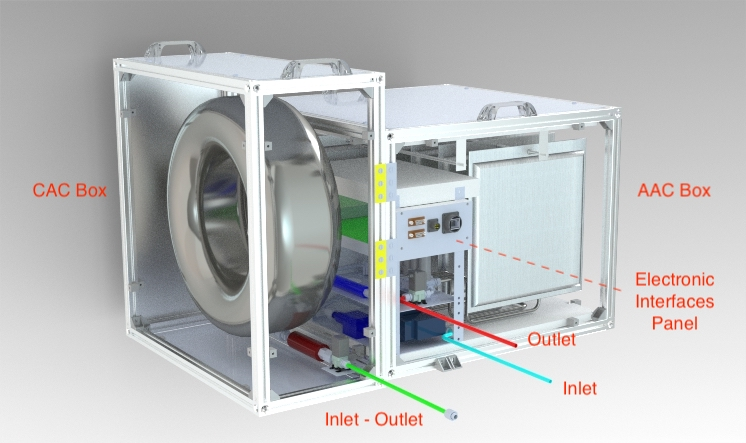
\includegraphics[width=1\linewidth]{4-experiment-design/img/Mechanical/v9_3D.jpg}
    \end{align*}
    \caption{Physical Setup of the Experiment.}
    \label{fig:3D_tubular_render}
\end{figure}

\begin{figure}[H]
    \begin{align*}
        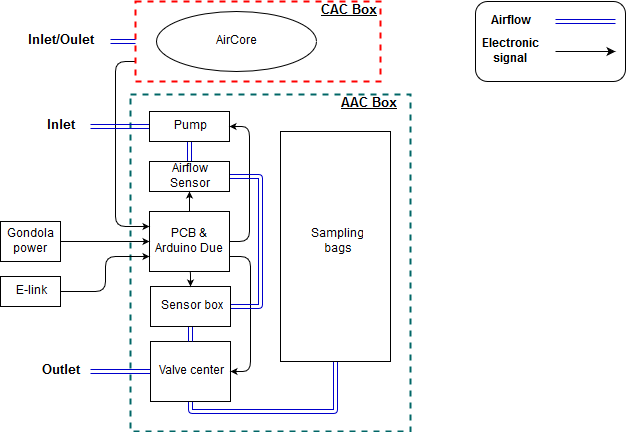
\includegraphics[width=1\linewidth]{4-experiment-design/img/Mechanical/Block-Diagram.png}
    \end{align*}
    \caption{Block Diagram of the Experiment.}
    \label{fig:block-diagram}
\end{figure}

The primary concern regarding the AAC air sampling subsystem occurs after the cut-off when the gondola will tumble and fall at an average speed of 50 m/s for approximately two minutes \cite{BexusManual}. This descent speed is too large in order to sample air at the desired vertical resolution, capped at 500 m. As such, sampling can only be done after the gondola has stabilized at a descent speed  of 8 m/s \cite{BexusManual}. The tumbling phase will vertically span for approximately 6 km. Considering a Float Phase altitude of 25 km, sampling during the Descent Phase will commence at approximately 19 km in altitude. However, the primary region of interest in terms of sampling is in the stratosphere, particularly between 19 km and 25 km in altitude. Sampling will thus also occur during the Ascent Phase. Out of the six sampling bags present in the payload, two will be used during the Ascent Phase at 18 km and 21 km and four during the Descent Phase at 17.5 km, 16 km, 14 km and 12 km as seen in Table \ref{tab:minimum-volume}. Details regarding the sampling strategy can be found in Appendix \ref{sec:appH}.

%\begin{table}[H]
\centering
\begin{tabular}{|c|c|c|c|}
\hline
\multicolumn{1}{|l|}{} & \multicolumn{1}{l|}{\textbf{Sampling Altitudes}} & \multicolumn{1}{l|}{\textbf{Ambient Pressure}} & \multicolumn{1}{l|}{\textbf{Ambient Temperature}} \\ \hline
\multirow{2}{*}{\textbf{Ascent Phase}} & 18 km & 75.0 hPa & 216.7 K \\ \cline{2-4} 
 & 21 km & 46.8 hPa & 217.6 K \\ \hline
\multirow{4}{*}{\textbf{Descent Phase}} & 17.5 km & 81.2 hPa & 216.7 K \\ \cline{2-4} 
 & 16 km & 102.9 hPa & 216.7 K \\ \cline{2-4} 
 & 14 km & 141.0 hPa & 216.7 K \\ \cline{2-4} 
 & 12 km & 193.3 hPa & 216.7 K \\ \hline
\end{tabular}
\caption{Sampling Altitudes as well as the Corresponding Ambient Pressures and Temperatures According to the 1976 US Standard Atmosphere.}
\label{tab:sampling-altitudes}
\end{table}
The maximum pressure that the sampling bags can withstand has to be taken into account in order to avoid bursting. Decreasing pressure during the Ascent Phase poses a risk to sampling bags which already contain samples as the gas inside will expand which may cause the bag to burst. In order to avoid this, the sampling bags will not be completely filled. Filling up to a maximum of 80\% of the sampling bag's capacity (2 psi/0.14 bar) is recommended by the manufacturers for the Multi-Layer Foil sampling bags that are to be used. Therefore, the maximum expected pressure inside the bags, that will be filled during the Ascent Phase, will be 1.6 psi/0.11 bar. The inverse is also true for the Descent Phase where compression will occur. As such, the sampling bags should be fully filled during the Descent Phase in order to ensure that enough samples are collected for analysis. During the Descent Phase, the maximum pressure inside the bags is expected to be 1.98 psi/0.13 bar. Past research has revealed that the selected sampling bags can withstand pressure difference of 310 hPa at 30 km of altitude, which is equivalent to 0.31 bar \cite{LISA}. A series of tests listed in Table \ref{tab:sampling-system-test} will be conducted in order to confirm the maximum allowable pressure for the bags.

The maximum operating pressure for the tubes, according to the manufacturers, is 2.2 psi/0.15 bar. The valve's leakage rate, given by the manufacturers, is 0.001 l/min.     


Due to the difference in pressure between sea level and sampling altitudes, the volume of the sample taken will be considerably reduced when it reaches sea level. This shrinking has to be taken into account as the minimum volume that has to be present in the sampling bag at ground level in order to obtain results with the Picarro analyzer. A minimum amount is required for the analyzer to detect concentrations of the targeted trace gases. This minimum amount is 0.18 L at sea level and it has to be specially considered for the samples taken at higher altitudes. The samples taken at lower altitudes will be exposed to smaller changes in pressure, therefore their size will not be critically reduced. Table \ref{tab:minimum-volume} shows the minimum volume of air that needs to be sampled at different altitudes and the corresponding temperature and pressure conditions, in order the sample volume left at sea level pressure and temperature (288 K)  is at least 0.18L.  

% Depending on the sampling altitude,there is a minimum volume of air that needs to be sampled in order the sample volume left at sea level pressure is at least 0.18 L. A sample volume of 0.18 L corresponds to the minimum amount required for the Picarro analyzer to detect concentrations of the targeted trace gases. 

% Please add the following required packages to your document preamble:
% \usepackage{multirow}
\begin{table}[H]
\centering
\begin{tabular}{|l|l|l|l|l|}
\hline
 & \textbf{\begin{tabular}[c]{@{}l@{}}Minimum \\ Sampling Volume\end{tabular}} & \textbf{\begin{tabular}[c]{@{}l@{}}Sampling \\ Altitudes\end{tabular}} & \textbf{\begin{tabular}[c]{@{}l@{}}Ambient \\ Pressure\end{tabular}} & \textbf{\begin{tabular}[c]{@{}l@{}}Ambient \\ Temperature\end{tabular}} \\ \hline
\multirow{2}{*}{\textbf{Ascent Phase}} & 1.8 L & 18 km & 75.0 hPa & 216.7 K \\ \cline{2-5} 
 & 2.4 L & 21 km & 46.8 hPa & 217.6 K \\ \hline
\multirow{4}{*}{\textbf{Descent Phase}} & 1.7 L & 17.5 km & 81.2 hPa & 216.7 K \\ \cline{2-5} 
 & 1.3 L & 16 km & 102.9 hPa & 216.7 K \\ \cline{2-5} 
 & 1.0 L & 14 km & 141.0 hPa & 216.7 K \\ \cline{2-5} 
 & 0.7 L & 12 km & 193.3 hPa & 216.7 K \\ \hline
\end{tabular}
\caption{Sampling Altitudes as well as the Corresponding Ambient Pressures and Temperatures According to the 1976 US Standard Atmosphere and the Minimum Sampling Volume at Each Altitude to Obtain Enough Air to Perform a Proper Analysis (0.18 L at Sea Level), Appendix \ref{sec:appH}.}
\label{tab:minimum-volume}
\end{table}


The AAC will need an air pump for sampling due to low ambient pressure at stratospheric altitudes. The air pump is also needed in order to assure the intake flow rate and obtain a good resolution. An air pump with an intake rate of at least 3 L/min will be used to ensure that the vertical resolution of the sampling air remains under 500 m during the Ascent Phase's ascent speed of 5 m/s and the  Descent Phase's descent speed of 8 m/s. A flushing valve (see Figure \ref{pneumatic_system}, No.23) will be used to flush the AAC system before each bag is filled and make sure that each bag will be filled with fresh air from the corresponding altitude. This filling/flushing procedure occurs twice, the first time during the Ascent Phase for the first two sampling bags and the second time during the Descent Phase for the remaining four sampling bags.

Shortly after the launch, the CAC valve will be opened in order to allow the fill gas that is inside the tube to flush, while the AAC valves will be closed until reaching the sampling altitude. Flushing of the CAC tube happens passively through the progressive decrease in air pressure during the balloon's Ascent Phase and it will be emptied by the time it reaches the Float Phase. Filling of the CAC tube also happens passively through the progressive increase in air pressure during the balloon's Descent Phase. The CAC valve will remain open at all time during the Ascent, Float, and Descent phases. The valve will close just before hitting the ground in order to preserve the sample. 

The ambient pressure will be measured by three pressure sensors located outside the experiment box. Only one of them is necessary for AAC and CAC, but using three will provide redundancy. To measure the pressure inside the bag that is currently being filled, three more sensors will be allocated inside the sensors box. To measure the ambient temperature in the CAC, three sensors will be allocated in the CAC box (in the Styrofoam). Temperature inside the coil is assumed to quickly adjust to the ambient temperature inside the CAC box, therefore there will not be differentiation in temperature between the air inside the tube and the air surrounding the tube. For the bags three more temperature sensors will be placed in the bags' box (in the Styrofoam). To control the temperature for the Arduino, the pump and the valves in pneumatic subsystem, one temperature sensor will be used for each of them. In total, there will be six pressure sensors and nine temperature sensors. 

The sampling of the AAC will be triggered by the pressure reading from the sensors outside the experiment box. When the required pressure is reached, Table \ref{tab:minimum-volume}the valve inside the manifold corresponding to the bag that is to be sampled, will open and the sampling will start. The closing of the valve depends on two conditions and it will be triggered when either one of the conditions is true. These conditions are: maximum sampling time or maximum pressure difference between inside/outside the bags. They are determined from past research \cite{LISA}. A first estimation of the maximum sampling time has already been made, from Test 18 shown in Table \ref{tab:pump-low-pressure-test}, but more tests in the future will determine the maximum pressure condition and confirm the maximum sampling times.

The CAC emptying as well as the AAC and CAC sampling sequence is represented in Figures \ref{fig:ascent} and \ref{fig:descent}. It should be kept in mind that the different pressures are what triggers the opening of the valves. 

\begin{figure}[H]
    \begin{align*}
        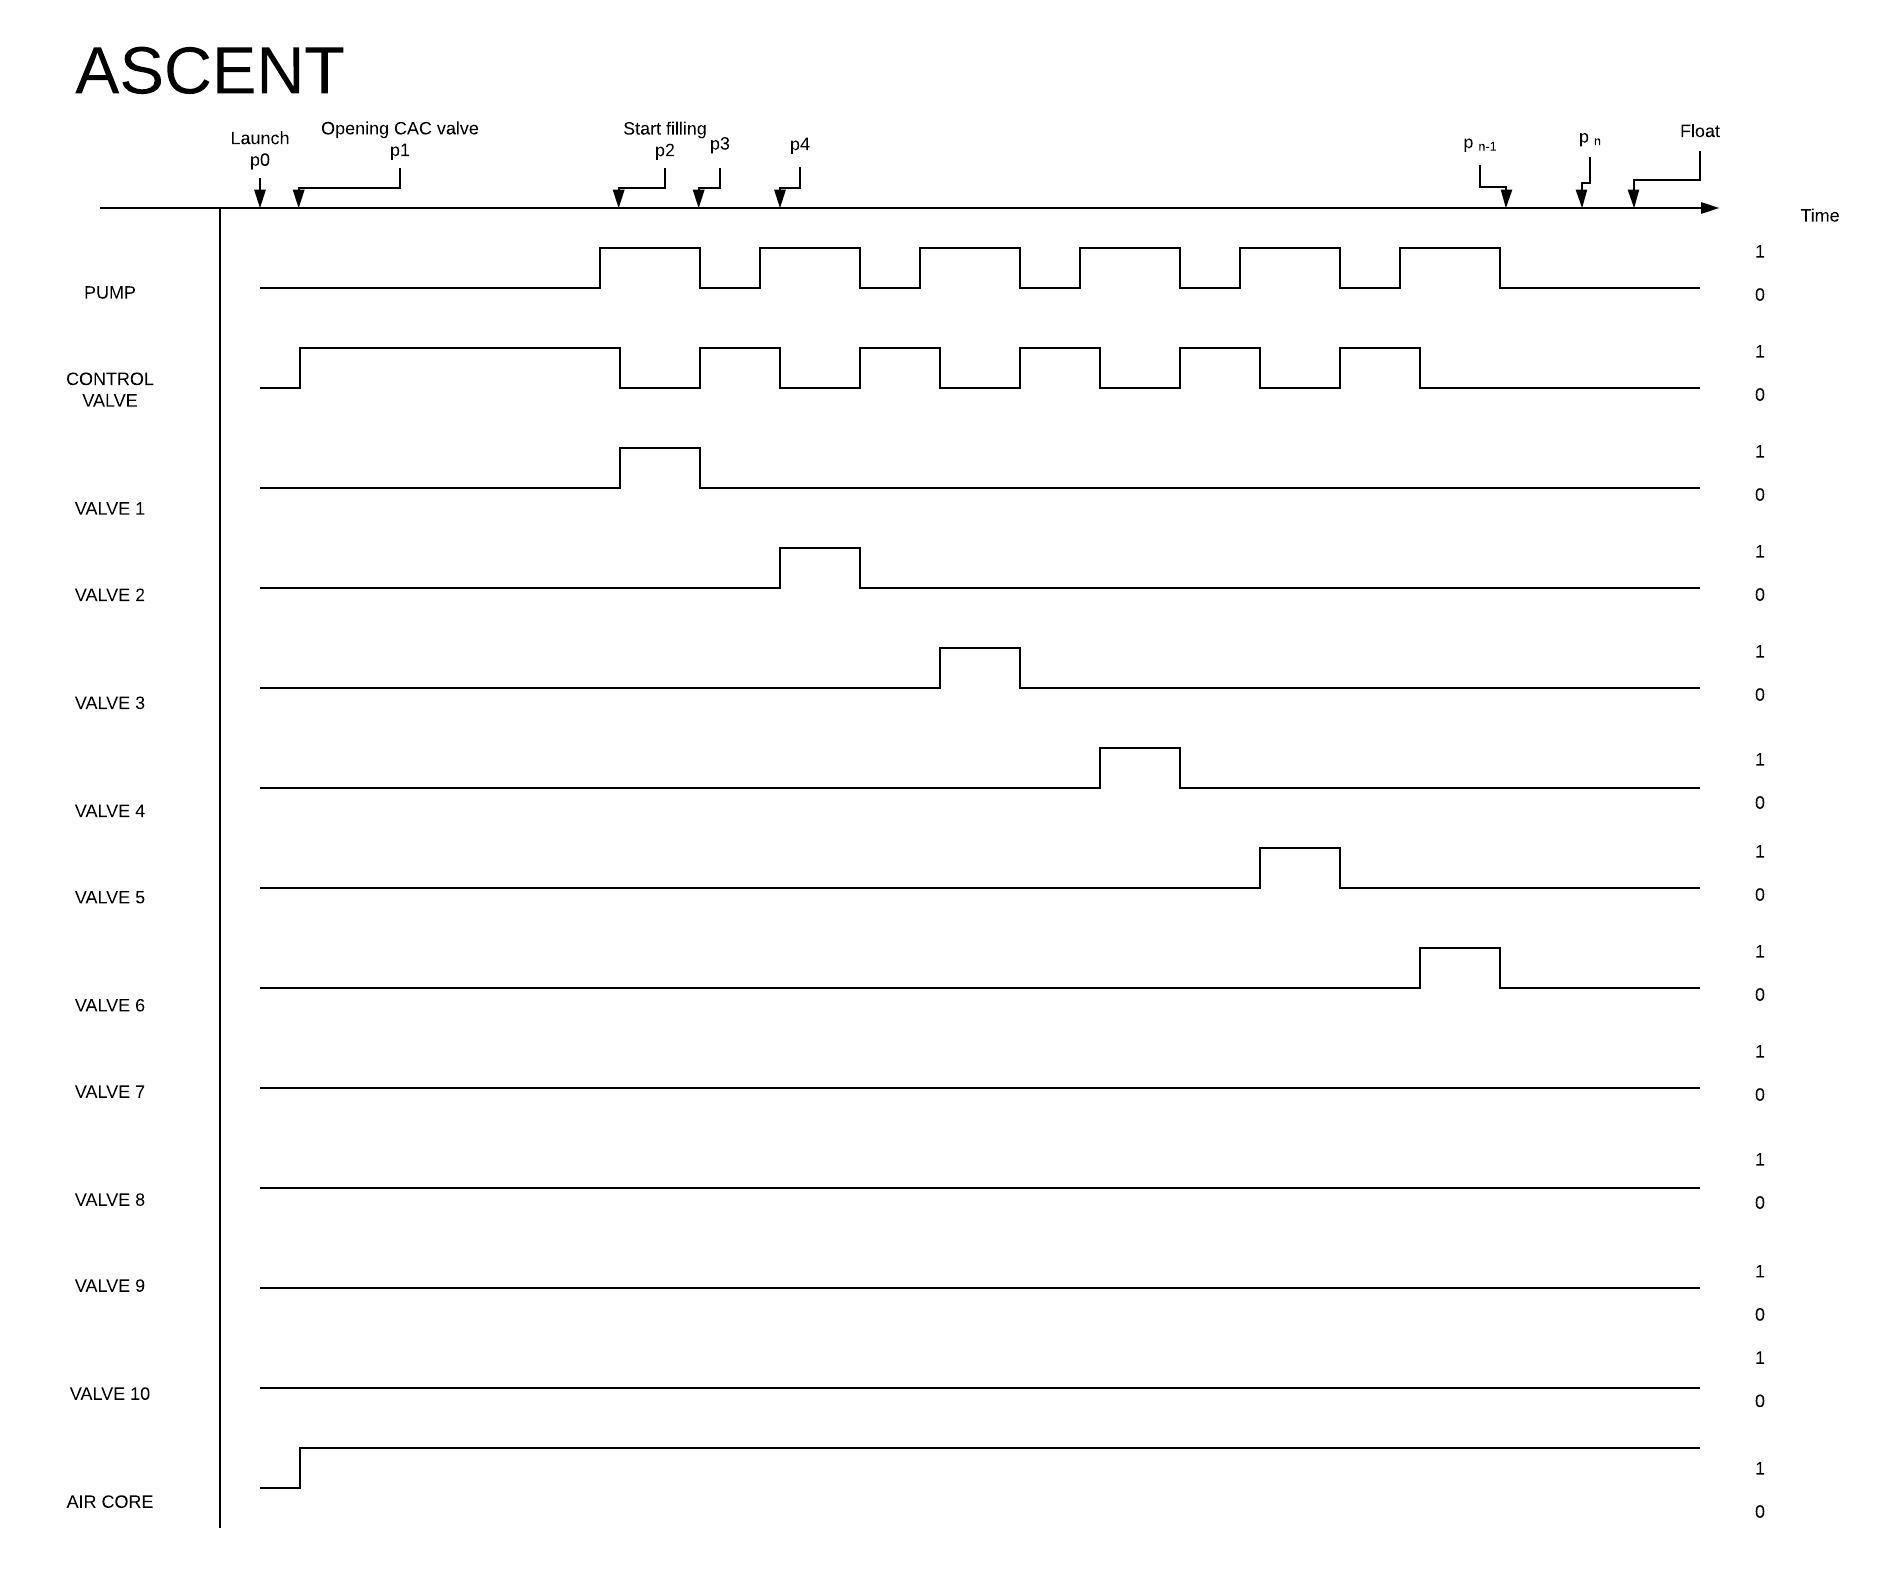
\includegraphics[width=1\linewidth]{4-experiment-design/img/ascent-phase.jpeg}
    \end{align*}
    \caption{The Emptying and Sampling Sequence-Ascent Phase.}
    \label{fig:ascent}
\end{figure}

\begin{figure}[H]
    \begin{align*}
        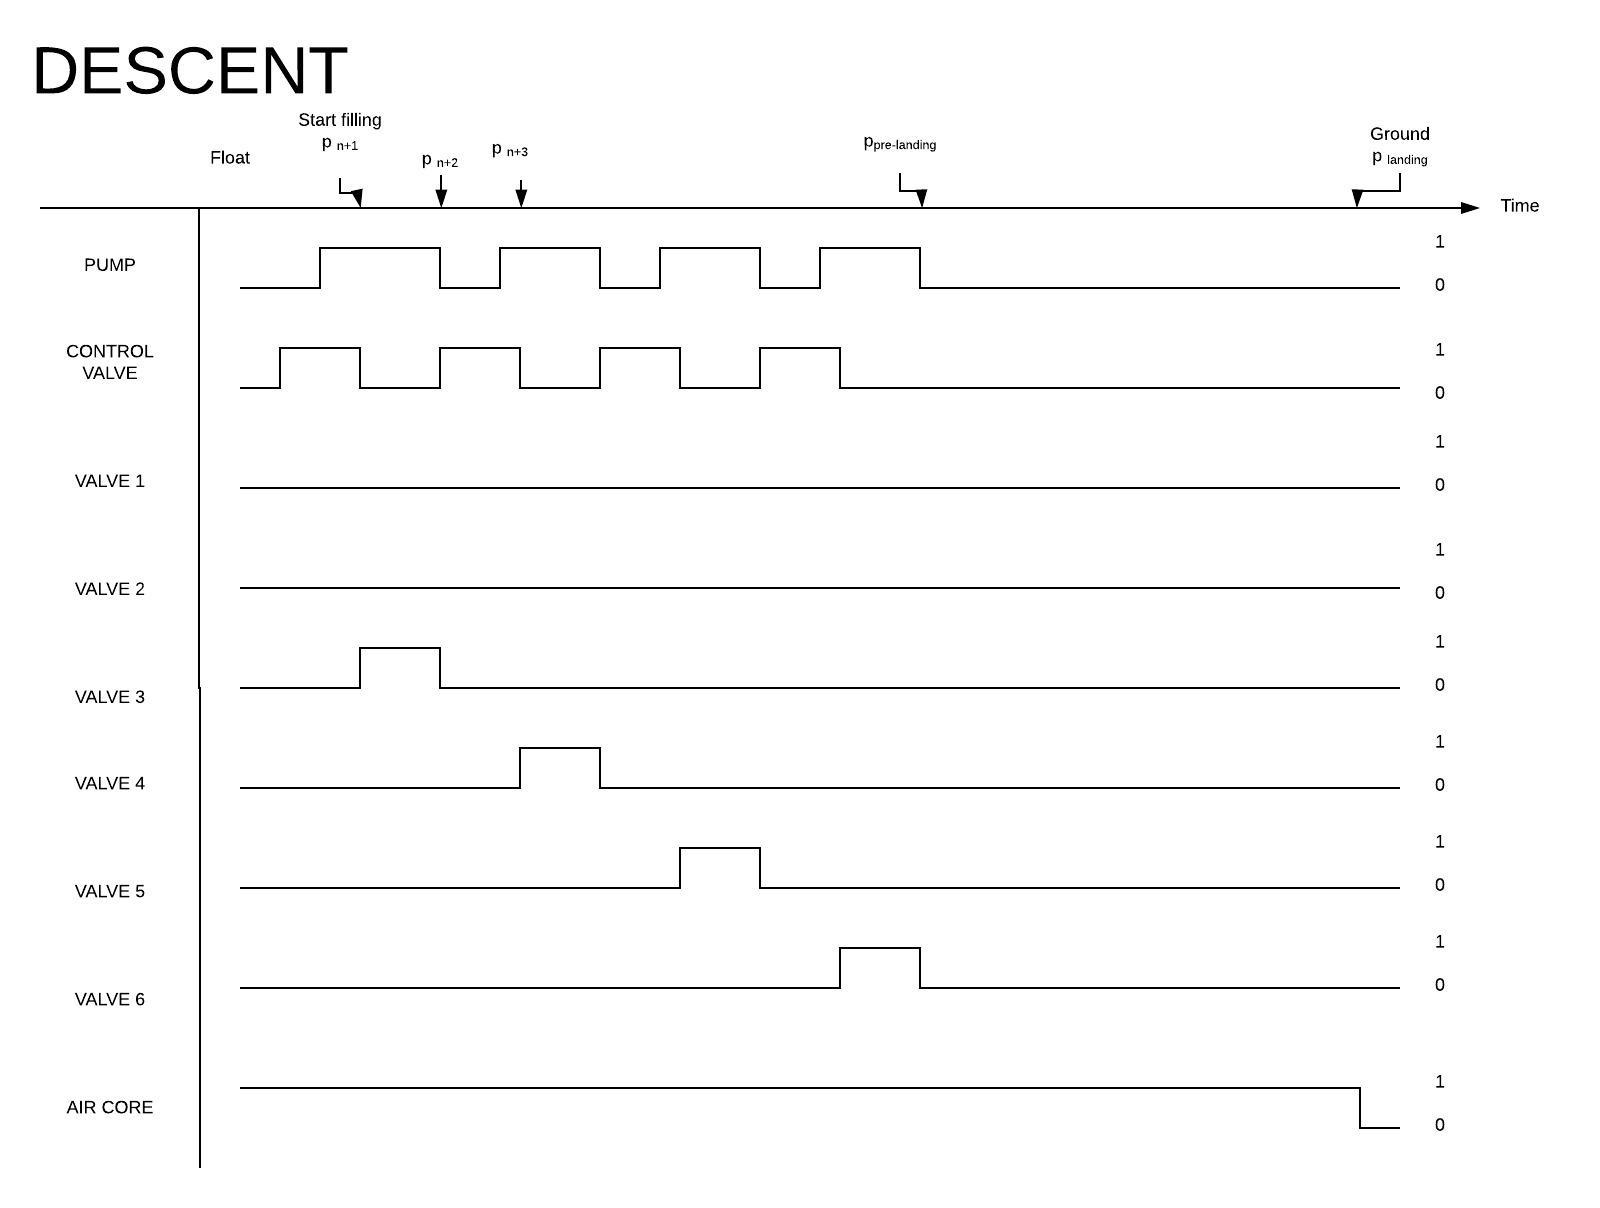
\includegraphics[width=1\linewidth]{4-experiment-design/img/descent-phase.jpeg}
    \end{align*}
    \caption{The Emptying and Sampling Sequence-Descent Phase.\label{fig:descent}}
\end{figure}

In the diagrams, 0 denotes closed/off and 1 denotes opened/on. The horizontal axis denotes the different pressure levels throughout the flight, with p$_0$ being the sea level pressure and p$_8$ being the pressure during Float Phase.

The ambient pressure dependent timeline of the experiment is as follow:

\textbf{Ascent Phase:}\\
$p_0$ – $p_1$
\begin{itemize}
    \item CAC valve shall be closed.
    \item AAC valves shall be closed.
    \end{itemize}
$p_1$ – $p_2$
\begin{itemize}
    \item CAC valve shall be opened.
    \item CAC tube shall start flushing.
    \end{itemize}

$p_2$ – $p_3$
\begin{itemize}
    \item AAC flushing valve shall be opened, allowing for the system to flush.
    \item CAC valve remains open.
    \end{itemize}
$p_3$ – $p_4$
\begin{itemize}
    \item AAC flushing valve shall be closed.
    \item Valve 1 shall be opened, allowing for air to enter the first bag.
    \item CAC valve remains open.
    \end{itemize}
$p_4$ – $p_5$
\begin{itemize}
    \item Valve 1 shall be closed.
    \item AAC flushing valve shall be closed.
    \item CAC valve remains open.
    \end{itemize}
$p_5$ - $p_6$    
 \begin{itemize}
    \item AAC flushing valve shall be opened, allowing the system to flush. 
    \item CAC valve remains open.
    \end{itemize}
$p_6$ - $p_7$
\begin{itemize}
    \item AAC flushing valve shall be closed.
    \item Valve 2 shall be opened, allowing for air to enter the second bag.
    \item CAC valve remains open.
    \end{itemize}
$p_7$ - $p_8$
\begin{itemize}
    \item Valve 2 shall be closed.
    \item AAC flushing valve shall be closed.
    \item CAC shall finish flushing.
    \end{itemize}    




\textbf{\\Float Phase:}\\
No action is taken other than continued telemetry.

\textbf{Descent Phase:}

$p_9$ – $p_{10}$
\begin{itemize}
    \item CAC shall start sampling. 
    \item AAC valves shall be closed.
\end{itemize}

$p_{10}$ – $p_{11}$
\begin{itemize}
    \item AAC flushing valve shall be opened allowing the system to flush.
    \item CAC valve remains open. 
\end{itemize}

  
$p_{11}$ – $p_{12}$
\begin{itemize}
    \item AAC flushing valve shall be closed.
    \item Valve 3 shall be opened, allowing for air to enter the third bag.
    \item CAC valve remains open. 
\end{itemize}

$p_{12}$ – $p_{13}$
\begin{itemize}
    \item Valve 3 shall be closed.
    \item AAC flushing valve shall be closed.
    \item CAC valve remains open.
\end{itemize}

$p_{13}$ – $p_{14}$
\begin{itemize}
    \item AAC flushing valve shall be opened allowing the system to flush.
    \item CAC valve remains open.
\end{itemize}

$p_{14}$ – $p_{15}$
\begin{itemize}
    \item AAC flushing valve shall be closed.
    \item Valve 4 shall be opened, allowing for air to enter the fourth bag.
    \item CAC valve remains open.
\end{itemize}

$p_{15}$ – $p_{16}$
\begin{itemize}
    \item Valve 4 shall be closed.
    \item AAC flushing valve shall be closed.
    \item CAC valve remains open.
\end{itemize}

$p_{16}$ – $p_{17}$
\begin{itemize}
    \item AAC flushing valve shall be opened, allowing the system to flush. 
    \item CAC remains open.
  \end{itemize}

$p_{17}$ – $p_{18}$
\begin{itemize}
    \item AAC flushing valve shall be closed.
    \item Valve 5 shall be opened, allowing for air to enter the fifth bag. 
    \item CAC valve remains open.
\end{itemize}

$p_{18}$ – $p_{19}$
\begin{itemize}
    \item Valve 5 shall be closed.
    \item AAC flushing valve shall be closed.
    \item CAC valve remains open.
\end{itemize}

$p_{19}$ – $p_{20}$
\begin{itemize}
     \item AAC flushing valve shall be opened, allowing the system to flush. 
    \item CAC remains open.
   \end{itemize}

$p_{20}$ – $p_{21}$
\begin{itemize}
    \item AAC flushing valve shall be closed.
    \item Valve 6 shall be opened, allowing for air to enter the sixth bag.
\end{itemize}

$p_{pre-landing}$ 
\begin{itemize}
    \item Valve 6 shall be closed.
    \item AAC flushing valve shall be closed.
    \item CAC valve shall be opened.
\end{itemize}

$p_{0-landing}$
\begin{itemize}
    \item CAC valve shall be closed.
\end{itemize}


Note: The AAC system's air pump is only on during sampling into the air sampling bags and flushing of the system.


\raggedbottom
\pagebreak
\subsection{Experiment Interfaces}

\subsubsection{Mechanical Interfaces}
\label{sec:4.2.1}

\bigskip
\begin{table}[H]
\noindent\makebox[\columnwidth]{%
\scalebox{0.8}{
\begin{tabular}{|c|c|c|c|c|c|}
\hline
\textbf{Component} & \textbf{Interface} & \textbf{Amount} & \textbf{Dimensions} & \textbf{Weight/unit} & \textbf{Total weight} \\ \hline
Bracket standard 20/20 slot 6/6 & AAC-Gondola & $8$ & $20 \times 20 \times 20\ mm$ & $5\ g$ & $40\ g$ \\ \hline
Tolerance holes bracket & CAC-Gondola & $2$ & $ 20 \times 30 \times 52 \ mm$ & $20\ g$ & $40\ g$ \\ \hline
6-hole plate & AAC-CAC & $4$ & $1 \times 60 \times 41\ mm$ & $50\ g$ & $200\ g$ \\ \hline
Rubber bumpers M6 & AAC-Gondola, CAC-Gondola & $10$ & $19 \times 19 \times 15\ mm$ & $30\ g$ & $300\ g$ \\ \hline
T-nut slot 6 M4 & AAC-CAC, AAC-Gondola, CAC-Gondola & $34$ & $4 \times 5.9 \times 11.5\ mm$ & $3\ g$ & $102\ g$ \\ \hline
T-nut slot 8 M6 & AAC-Gondola, CAC-Gondola & $10$ & $6 \times 11 \times 16\ mm$ & $6\ g$ & $60\ g$ \\ \hline

Steel bolt M4 & AAC-CAC, AAC-Gondola & $34$ & $8\ mm $ length & $1\ g$ & $34\ g$ \\ \hline
Steel washer M4 & AAC-CAC, AAC-Gondola & $24$ &\begin{tabular}[c]{@{}c@{}}$ID=4.3\ mm$\\ $OD=9\ mm$\end{tabular} & $0.2\ g$ & $4.8\ g$\\ \hline
Polyamide bolt M4 & Styrofoam-CAC-AAC & $8$ & $20\ mm $ length & $3\ g$ & $24\ g$ \\ \hline
Polyamide washer M4 & Styrofoam-CAC-AAC & $8$ &\begin{tabular}[c]{@{}c@{}}$ID=4.3\ mm$\\ $OD=25\ mm$\end{tabular} & $4\ g$ & $32\ g$\\ \hline
Styrofoam bars  & AAC-Gondola, CAC-Gondola & $4$ & see Appendix \ref{sec:mech_drawings} & $-$ & $700\ g$ \\ \hline
Handles  & CAC \& AAC & $4$ & $ 18.6 \times 25.2 \times 112.5 \ mm$ & $20\ g$ & $80\ g$ \\ \hline
\end{tabular}}}
\caption{Summary of Gondola-AAC-CAC Interfaces Components.}
\label{table:attaching-components}
\end{table}


\underline{Gondola - TUBULAR joining}

\smallskip
The experiment box will be fixed to the gondola rails by means of $10$ brackets interfacing the experiment outside structure with the hammer nuts in the rails. Two different types of brackets are used to be flexible with respect to the gondola rails distances, which can be modified by use after previous BEXUS campaigns. Eight small $20/20$ brackets (Figure \ref{fig:bracket_small}) are used to fix the AAC box to specific rails placement, and two other big brackets (Figure \ref{fig:bracket_big}) are used to fix the CAC box to the nearest rail. This method is secure as well as fast enough to provide an accessible and easy recovery for later analysis.

\begin{figure}[H]
    \noindent\makebox[\textwidth]{%
    \begin{subfigure}{.3\textwidth}
        \centering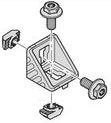
\includegraphics[width=0.55\textwidth]{4-experiment-design/img/Mechanical/bracket.jpg}
        \caption{Rexroth 20/20.}
        \label{fig:bracket_small}
    \end{subfigure}
    \hspace{1cm}
    \begin{subfigure}{.3\textwidth}
        \centering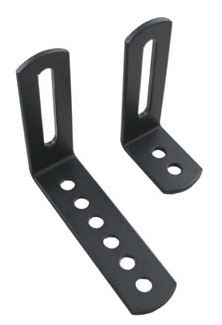
\includegraphics[width=0.55\textwidth,angle=90] {4-experiment-design/img/Mechanical/long_hole_bracket.jpg}
        \caption{Tolerance Holes.}
        \label{fig:bracket_big}
    \end{subfigure}}
    \caption{Bracket Components.}
    \label{fig:bracket}
\end{figure}

\bigskip
\underline{CAC - AAC joining}

\smallskip
A simple but reliable fixing interface between the two boxes of the experiment has been designed to ensure the fast recovery of the CAC box. The latter requires only unscrewing 12 bolts as well as unplugging a D-Sub connector. Once the CAC box is detached, the AAC Box will still remain perfectly fixed in the gondola. Table \ref{table:attaching-components} gathers up all the components required to fix the experiment to the gondola.

\bigskip
\underline{Handles}

\smallskip
Four top handles, as shown in Figure \ref{fig:handles} will be mounted to facilitate the experiment box manipulation when moving it in and out of the gondola.

\begin{figure}[H]
    \centering
    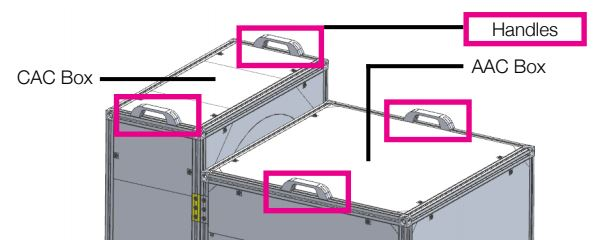
\includegraphics[width=0.8\textwidth]{4-experiment-design/img/Mechanical/handles.jpg}
    \caption{Handling Interfaces.}
    \label{fig:handles}
\end{figure}

\bigskip
\underline{Inlet/Outlet Pipes}
\label{subsec:pipes}

\smallskip
In order to collect reliable air samples, the experiment requires to be mounted at least with one side exposed to the outside. The later will reduce the pipe length used to collect clean air. As it can be seen in Figure \ref{fig:3D_tubular_render}, three pipes will extend from the experiment box face: one for the CAC sampling and two, input and output, for the AAC sampling. The one-way selected method will provide a proper flushing of the pipe and thus ensure a reliable sampling as explained in Section \ref{Experiment_Setup}.

These pipes are welded/drawn $304$ grade stainless steel tubes from RESTEK company, which are specially recommended for chromatography applications and gas delivery systems with low pressures and inert environments. These tubes are sulfinert, which is a required treatment for metal components when analyzing for parts-per-billion levels of organo-sulfur compounds.

The tubes, which are the same that will be used in the pneumatic system of the \emph{Brain} (see Section \ref{sec:4.4.5}), have an outer diameter $OD = 6.35\ mm$ ($1/4$ inches) and an inner diameter $ID = 4.57\ mm$ ($0.18$ inches).

\subsubsection{Thermal Interfaces}
\label{sec:4.2.2}

Both main structural components and external walls of the two boxes of the experiment are made by aluminum and steel components. For this reason, since these are conductive materials, a direct attachment to the gondola creates many heat paths with the internal space and subsystems of the experiment. Considering that the temperature gradient between the gondola and the operative requirements of the electronic components can be quite high, this conductive connections drastically decrease the efficiency of the thermal insulation. Therefore, a system based on rubber bumpers and styrofoam bars (see Figure \ref{fig:thermal_interface}) has been designed to add heat bridges and minimize temperature leaks from the inside of the experiment to the outside.

Figure \ref{fig:rubber_bumper} shows a CAD model of the bumper component and how it looks like when attached to the gondola with the brackets explained in the previous section.

\begin{figure}[H]
    \noindent\makebox[\textwidth]{%
    \begin{subfigure}{.3\textwidth}
        \centering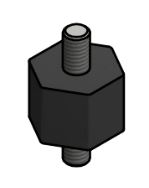
\includegraphics[width=0.55\textwidth]{4-experiment-design/img/Mechanical/rubber_bumper.jpg}
    \end{subfigure}
    \hspace{1cm}
    \begin{subfigure}{.3\textwidth}
        \centering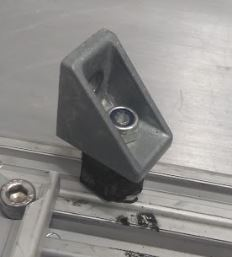
\includegraphics[width=0.55\textwidth] {4-experiment-design/img/Mechanical/real_bumper.jpg}
    \end{subfigure}}
    \caption{Rubber Bumper.}
    \label{fig:rubber_bumper}
\end{figure}

The styrofoam bars will be attached directly to the rails of the experiment structure by M4 plastic screws and big washers.

\begin{figure}[H]
    \centering
    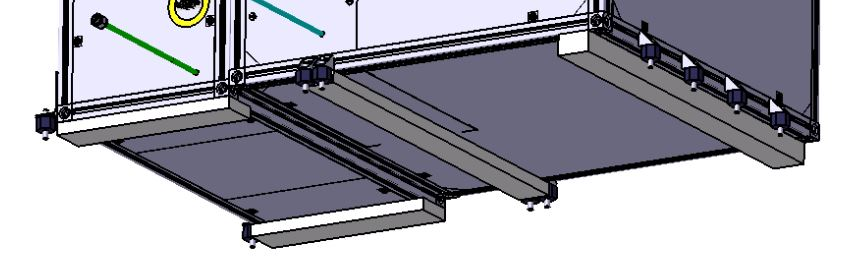
\includegraphics[width=0.8\textwidth]{4-experiment-design/img/Mechanical/thermal_interfaces.jpg}
    \caption{Thermal Interfaces TUBULAR-Gondola.}
    \label{fig:thermal_interface}
\end{figure}

\subsubsection{CAC Interfaces}
An uncoupled quick connector, shown in Figure \ref{fig:Quick-connector-body}, will be attached at each end of the coiled tube to seal the opening. It will remain tightly sealed until the quick connectors are manually coupled. 

\begin{figure}[H]
    \centering
    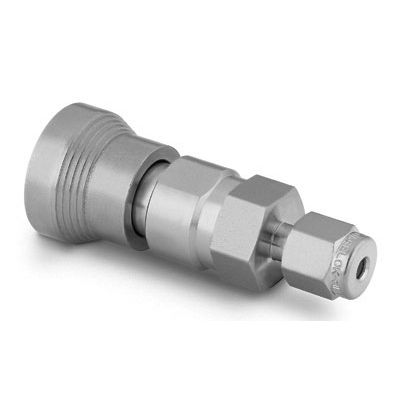
\includegraphics[width=0.2\textwidth]{4-experiment-design/img/Mechanical/CAC-QC-Outlet.jpg}
    \caption{Swagelok Quick Connector Body.}
    \label{fig:Quick-connector-body}
\end{figure}

The interfaces between the other parts in the CAC set up will be joined with specific tube fittings, listed in Table \ref{tab:CAC-interfaces}. All the chosen interfaces are from Swagelok. Using products from the same manufacture minimize the risk for leakage or mismatched interfaces in the system. 

\begin{table}[H]
\centering
\scalebox{0.8}{
\begin{tabular}{|c|c|c|c|}
\hline
\textbf{Component}                                                          & \textbf{Interface}             & \textbf{Amount} & \textbf{Fitting Size}                                                    \\ \hline
\begin{tabular}[c]{@{}c@{}}Quick connector body\\ SS-QC4-B-200\end{tabular} & Outlet of coiled tube          & 1               & 1/8 in.                                                                  \\ \hline
\begin{tabular}[c]{@{}c@{}}Quick connector body\\ SS-QC4-B-400\end{tabular} & Inlet of coiled tube           & 1               & 1/4 in.                                                                  \\ \hline
\begin{tabular}[c]{@{}c@{}}Quick connector stem\\ SS-QC4-D-400\end{tabular} & Inlet of coiled tube -  Filter & 1               & 1/4 in.                                                                  \\ \hline
\begin{tabular}[c]{@{}c@{}}Reducing adapter\\ SS-4-RA-2\end{tabular}        & Filter - Solenoid valve        & 1               & \begin{tabular}[c]{@{}c@{}}Female 1/4 in.\\ to male 1/8 in.\end{tabular} \\ \hline
\begin{tabular}[c]{@{}c@{}}Tube screw\\ SS-400-1-2\end{tabular}             & Solenoid valve - Exit tube     & 1               & \begin{tabular}[c]{@{}c@{}}1/8 in. to \\ tube OD 1/4 in.\end{tabular}    \\ \hline
\end{tabular}}
\caption{Interfaces within CAC Setup.}
\label{tab:CAC-interfaces}
\end{table}

\subsubsection{AAC Interfaces}
In the AAC system, the interfaces between various components are a mixture of five different types of tube fittings from Swagelok. The selected types are straight union, T-union, male elbow, female and male connectors with a certain  size, shown in Figure \ref{fig:AAC-interfaces-fittings}. Information regarding the fitting's placement in the AAC and fitting sizes are summarized in Table \ref{tab:AAC-interfaces}. 

\begin{figure}[H]
    \centering
    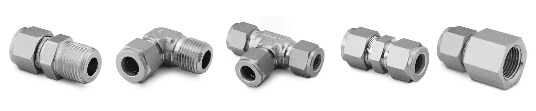
\includegraphics[width=0.8\textwidth]{4-experiment-design/img/Mechanical/AAC-interfaces.jpg}
    \caption{From Left to Right: Male Connector, Male Elbow, T-union, Straight Union and Female Connector.}
    \label{fig:AAC-interfaces-fittings}
\end{figure}

\begin{table}[H]
\centering
\scalebox{0.9}{
\begin{tabular}{|c|c|c|c|}
\hline
\textbf{Component}                                                    & \textbf{Interface}                                                                                                                                                                         & \textbf{Amount} & \textbf{Fitting Size}                                                                     \\ \hline
\begin{tabular}[c]{@{}c@{}}Male connector\\ SS-400-1-2\end{tabular}   & \begin{tabular}[c]{@{}c@{}}Airflow sensor - Sensor box\\ Tube sensor box - Manifold \\ Manifold - Flushing valve\\ Flushing valve - Outlet tube\\ Solenoid valve - Tube valve\end{tabular} & 11              & \begin{tabular}[c]{@{}c@{}}Male 1/8 in. to \\ Tube OD 1/4 in.\\ ID 0.21 in.\end{tabular}  \\ \hline
\begin{tabular}[c]{@{}c@{}}Male elbow\\ SS-400-2-2\end{tabular}       & Sensor box - Tube sensor box                                                                                                                                                               & 1               & \begin{tabular}[c]{@{}c@{}}Male 1/8 in. to \\ Tube OD 1/4 in.\\ ID 5/32 in.\end{tabular}  \\ \hline
\begin{tabular}[c]{@{}c@{}}Straight union\\ SS-400-6\end{tabular}     & \begin{tabular}[c]{@{}c@{}}Filter - Tube filter\\ Tube filter - Pump\\ Pump - Tube pump\end{tabular}                                                                                       & 3               & \begin{tabular}[c]{@{}c@{}}Tube OD 1/4 in.\\ ID 5/32 in.\end{tabular}                     \\ \hline
\begin{tabular}[c]{@{}c@{}}Female connector\\ SS-400-7-4\end{tabular} & \begin{tabular}[c]{@{}c@{}}Inlet tube - Filter\\ Tube pump - Airflow sensor\\ Airflow sensor - Tube airflow sensor\end{tabular}                                                            & 3               & \begin{tabular}[c]{@{}c@{}}Female 1/4 in. to\\ Tube OD 1/4 in.\\ ID 5/32 in.\end{tabular} \\ \hline
\begin{tabular}[c]{@{}c@{}}T-Union\\ SS-400-3\end{tabular}            & Tube valve - Bag valve                                                                                                                                                                     & 6               & Male 1/4 in.                                                                              \\ \hline
\end{tabular}}
\caption{Interface Descriptions Inside AAC System.}
\label{tab:AAC-interfaces}
\end{table}


\subsubsection{Electrical Interfaces}
\label{sec:4.2.3}

The experiment will connect to the gondola electrically via a 4 pin, male, box mount receptacle MIL - C-26482P series 1 connector with an 8-4 insert arrangement (MS3112E8-4P) \cite{BexusManual}. It will connect to one 28.8 V/1 mA battery pack which consists of eight SAFT LSH20 batteries in series where each has a 5 A fuse\cite{BexusManual}. The expected maximum current is 1.1 A.

\begin{figure}[H]
    \centering
    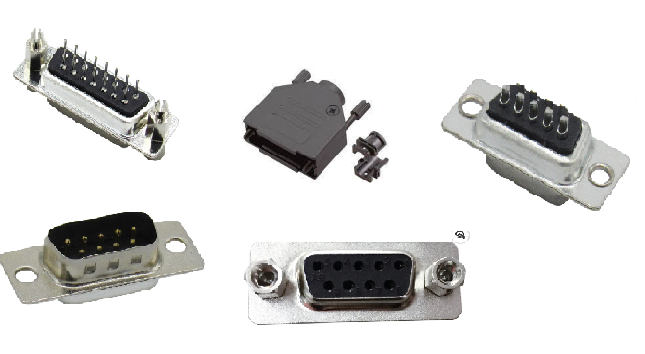
\includegraphics[width=0.4\textwidth]{4-experiment-design/img/connectors.png}
    \caption{Connectors.}
    \label{fig:connectors}
\end{figure}

The E-Link connection shall be made between the experiment and the E-Link system using a RJ45 connection which will be supplied by SSC and an Ethernet protocol. The Amphenol RJF21B connector will be mounted on either the front or the side of the experiment\cite{BexusManual}.  

The CAC and AAC will be connected together with a D-SUB 9-pin connector where power, ground and signals for the sensors in the CAC will be connected. A female connector will be located on the AAC wall and a male connector on the CAC wall.

Another female D-SUB 9-pin connector will be located on the wall of the AAC in which the connections for the three ambient pressure sensors will be located. Connectors with different pin configuration are shown in Figure \ref{fig:connectors}.

The expected data rate is 1.58 kbits/s for downlink and 1.08 kbits/s for uplink.



%\begin{figure}[H]
%    \begin{align*}
%        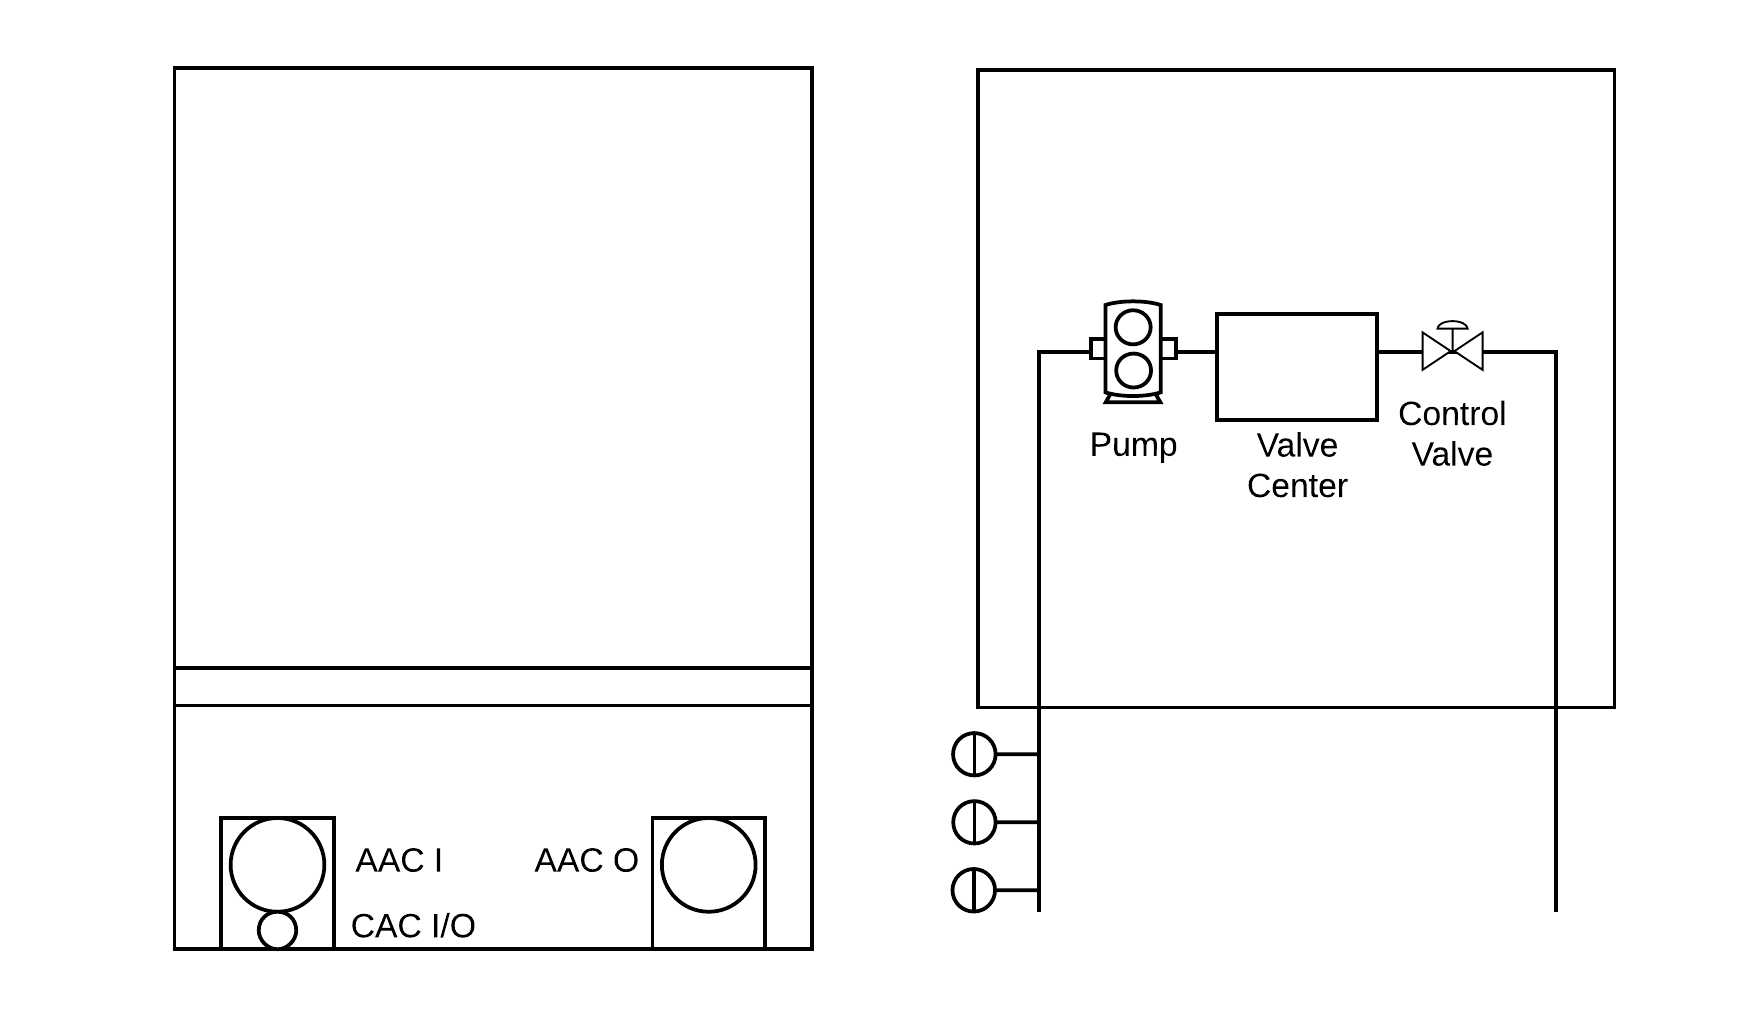
\includegraphics[width=0.7\textwidth]{4-experiment-design/img/Diagram_pipe.png}
%    \end{align*}
%    \caption{Diagram of the experiment box face exposed to the outside.}\label{fig:pipes_interface_1}
%\end{figure}

\iffalse
\subsubsection{Radio Frequencies (Optional)}
\begin{centering}
Not required.
\end{centering}
\bigskip

\subsubsection{Thermal (Optional)}
\begin{centering}
Not required.
\end{centering}
\bigskip
\fi


\raggedbottom
\begin{landscape}
\subsection{Experiment Components} \label{components}
\label{sec:experiment-components}

Component tables were generated from the project budget spreadsheet in Appendix \ref{sec:appO} using the scripts included in Appendix \ref{sec:appK}. Table headers are letter coded and correspond to the following:

\DIFdelbegin \textbf{\DIFdel{A}} %DIFAUXCMD
\DIFdel{- Components Name}%DIFDELCMD < \\
%DIFDELCMD < %%%
\textbf{\DIFdel{B}} %DIFAUXCMD
\DIFdel{- Manufacturer}%DIFDELCMD < \\
%DIFDELCMD < %%%
\textbf{\DIFdel{C}} %DIFAUXCMD
\DIFdel{- Manufacturer Code}%DIFDELCMD < \\
%DIFDELCMD < %%%
\textbf{\DIFdel{D}} %DIFAUXCMD
\DIFdel{- Quantity}%DIFDELCMD < \\
%DIFDELCMD < %%%
\textbf{\DIFdel{E}} %DIFAUXCMD
\DIFdel{- Total Cost }%DIFDELCMD < [%%%
\DIFdel{EUR}%DIFDELCMD < ]\\
%DIFDELCMD < %%%
\textbf{\DIFdel{F}} %DIFAUXCMD
\DIFdel{- Total Mass }%DIFDELCMD < [%%%
\DIFdel{g}%DIFDELCMD < ]\\
%DIFDELCMD < %%%
\textbf{\DIFdel{G}} %DIFAUXCMD
\DIFdel{- Note}%DIFDELCMD < \\
%DIFDELCMD < %%%
\textbf{\DIFdel{H}} %DIFAUXCMD
\DIFdel{- Status}%DIFDELCMD < \\
%DIFDELCMD < 

%DIFDELCMD < %%%
\DIFdelend \subsubsection{Electrical Components}

Table \ref{tab:components-table-electrical} shows all required electrical components with their total mass and price.\\


\begin{longtable} {|m{0.05\textwidth}|m{0.25\textwidth}|m{0.15\textwidth}|m{0.2\textwidth}|m{0.05\textwidth}|m{0.07\textwidth}|m{0.05\textwidth}|m{0.25\textwidth}|m{0.095\textwidth}|} \hline \textbf{ID} & \textbf{Component Name} & \textbf{Manufacturer} & \textbf{Manufacturer Code} & \textbf{Qty} & \textbf{Total Cost [EUR]} & \textbf{Total Mass [g]}  & \textbf{Note}  & \textbf{Status} \\ \hline E1 & Arduino Due & Arduino & A000062 & 1 & 36 & 35 & Fast and has many analog, and digital pins & Received \\ \hline E2 & Ethernet Shield & SEEED Studio & SKU 103030021 & 1 & 36 & 30 & Can be mounted on  top  of the board & Received \\ \hline E3 & Miniature diagphram air pump & KNF & NMP 850.1.2 KNDC-B & 1 & 430 & 350 &  & Received \\ \hline E4 & Pressure sensor & SENSOR SOLUTIONS & MS560702BA03-50 & 4 & 5 & 2.3 & High  resolution,  large  measuring range & Received \\ \hline E5 & Sampling Valve (inlet and outlet 1/8"" female) & SMC & VDW22UANXB & 1 & 100 & 45 & Estimated Arrival Date 27/7 & Ordered \\ \hline E6 & Airflow sensor & Honeywell & AWM5102VN & 1 & 60 & 130 & 0-10 SLPM & Received \\ \hline E7 & Heater & Minco & HK5160R157L12 & 4 & 4 & 95 & Easy to mount, compact size & Received \\ \hline E9 & Temperature sensor & Maxim Integrated & DS1631+-ND & 8 & 2 & 3 & I2C  digital  output interface, temperature  range  down  to -55 °C & Received \\ \hline E10 & DC/DC converter 24 V & Traco Power & S24SP24003PDFA & 2 & 46 & 49 & Provides required output voltage and power, 93\% efficiency & Received \\ \hline E11 & Humidity sensor & Texas Instrument & HDC2010	 & 3 & 5 & 3 & I2C interface, good temperature range, high accuracy & Received \\ \hline E12 & MicroSD & Kingston Technology & SDCIT/16GB & 1 & 0.5 & 20 & Small, good temperature range, sufficient storage & Received \\ \hline E13 & Logic CAT5E Network & Valueline & VLCT85000Y30 & 1 & 90 & 7 & For testing and ground station & Received \\ \hline E14 & Resistors (33 Ohm) \footnote{See schematic in Figure \ref{fig:Schematic} for details on where individual resistors are placed.} & n/a & n/a & 25 & 1 & 0 &  & Received \\ \hline E15 & Capacitors (0.1 uF, 5uF and 10 uF) & n/a & n/a & 15 & 1 & 0 &  & Received \\ \hline E16 & Mosfet for current control & IR & IRLB8748PBF & 11 & 2 & 0.7 & Cheap, good temperature range & Received \\ \hline E17 & Diodes for DCDC converters & Diotec Semiconductor & 1N5059 & 14 & 0.4 & 0.1 & Cheap, good temperature range & Received \\ \hline E18 & LED 3.3 V & Wurth Elektronik & 151034GS03000 & 16 & 0.4 & 0.52 & For monitoring, testing & Received \\ \hline E19 & 15-pin D-SUB Female connector with pins & RND Connect & RND 205-00779 & 2 & 11 & 0.75 & For connecting distributed components & Received \\ \hline E20 & 9-pin D-SUB Female connector with pins & RND Connect & RND 205-00777 & 3 & 8.5 & 0.68 & For connecting distributed components & Received \\ \hline E21 & 9 pin D-SUB Female connector with soldering cups & RND Connect & RND 205-00704 & 2 & 9 & 0.56 & For connecting distributed components & Received \\ \hline E22 & 9 pin D-SUB Male connector with soldering cups & RND Connect & RND 205-00700 & 4 & 9 & 0.48 & For connecting distributed components & Received \\ \hline E23 & 15-pin D-SUB Male connector with soldering cups & RND Connect & RND 205-00701 & 2 & 11 & 0.6 & For connecting distributed components & Received \\ \hline E24 & 9-pin D-SUB backing & Enchitech & MHDTZK-9-BK-K & 4 & 40 & 2.9 & For connecting distributed components & Received \\ \hline E25 & 15-pin D-SUB backing & Enchitech & MHDTZK-15-BK-K & 2 & 66 & 3.1 & For connecting distributed components & Received \\ \hline E26 & Wall mounting bolts & RND Connect & RND 205-00786 & 3 & 2.5 & 1 & For connecting distributed components & Received \\ \hline E27 & D-SUB cable CAC to AAC & Maxxtro & n/a & 1 & 80 & 3.8 & For connecting distributed components & Received \\ \hline E28 & 3.3 V Zener diode & RND Components & RND 1N746A & 15 & 0.5 & 0.07 & Regulate indication LED voltage & Received \\ \hline E29 & Male connector on PCB & Binder & Serie 768 & 1 & 5 & 8.5 &  & Received \\ \hline E30 & Female connector from wall & Binder & Serie 768 & 1 & 11 & 12 &  & Received \\ \hline E31 & Grounding contact & Vogt & DIN 46234 & 4 & 0.58 & 8.6 & 1 pack of 100 pcs & Received \\ \hline E32 & Logic CAT5 E-link for inside box & Valueline & VLCP85121E015 & 1 & 10 & 1.1 & To connect from wall to Arduino shield & Received \\ \hline E33 & Signal wire & Alpha Wire & 5854/7 YL005 & 1 & 230 & 34 & Roll of 30 m. Half will be used approximately & Received \\ \hline E34 & Flushing valve (inlet and outlet 1/8"" female) & SMC & VDW22UANXB & 1 & 100 & 45 & Estimated Arrival Date 27/7 & Ordered \\ \hline E35 & Valves manifold (outlet 1/8"" female) & SMC & VDW23-5G-1-H-Q & 6 & 100 & 40 & Estimated Arrival Date 27/7 & Ordered \\ \hline E36 & Power wire - Back & Alpha Wire & 5856 BK005 & 1 & 370 & 46 & Roll of 30 m. A fifth will be used approximately & Received \\ \hline E37 & Electrical Tape for marking wires - White & Hellerman Tyton & HTAPE-FLEX15WH-15X10 & 1 & 34 & 0.82 & Roll of 10 m. A forth will be used approximately & Received \\ \hline E38 & Electrical Tape for marking wires - Black & Hellerman Tyton & HTAPE-FLEX15BK-15X10 & 1 & 33 & 0.82 & Roll of 10 m. A forth will be used approximately & Received \\ \hline E39 & Electrical Tape for marking wires - Green & Hellerman Tyton & HTAPE-FLEX15GN-15X10 & 1 & 34 & 0.82 & Roll of 10 m. A forth will be used approximately & Received \\ \hline E40 & Electrical Tape for marking wires - Violet & Hellerman Tyton & HTAPE-FLEX15VT-15X10 & 1 & 34 & 0.82 & Roll of 10 m. A forth will be used approximately & Received \\ \hline E41 & Electrical Tape for marking wires - Gray & Hellerman Tyton & HTAPE-FLEX15GY-15X10 & 1 & 34 & 0.82 & Roll of 10 m. A forth will be used approximately & Received \\ \hline E42 & Electrical Tape for marking wires - Brown & Hellerman Tyton & HTAPE-FLEX15BN-15X10 & 1 & 34 & 0.82 & Roll of 10 m. A forth will be used approximately & Received \\ \hline E43 & Electrical Tape for marking wires - Blue & Hellerman Tyton & HTAPE-FLEX15BU-15X10 & 1 & 34 & 1.9 & Roll of 10 m. A forth will be used approximately & Received \\ \hline E48 & Power wire - Red & Alpha Wire & 5856 RD005 & 1 & 370 & 46 & Roll of 30 m. A fifth will be used approximately & Ordered \\ \hline E49 & Potentiometer 1 kOhm & Bourns & M64Y102KB40 & 4 & 1 & 1.8 &  & Received \\ \hline E50 & 6-pin male double row header & RND Connect & RND 205-00634 & 2 & 1 & 0.22 &  & Received \\ \hline E51 & 8-pin male single row header & RND Connect & RND 205-00629 & 5 & 1 & 0.28 &  & Received \\ \hline E52 & 10-pin male single row header & Prostar & SD-2X5-T1-7/3MM & 1 & 1 & 0.26 &  & Received \\ \hline E53 & 36-pin male double row header & Würth Elektronik & 61303621121 & 1 & 2 & 1.7 &  & Received \\ \hline E54 & DC/DC converter 12 V & Delta & R-7812-0.5 & 2 & 20 & 34 & 12V,1.67A, 20W DCDC & Received \\ \hline E55 & Potentiometer 50 kOhm & Bourns & 3296Y-1-503LF & 4 & 1 & 1.8 &  & Received \\ \hline E56 & Static Pressure Sensor & Gems Sensors and Controls & 3500S0001A05E000 & 1 & 53 & 140 &  & Waiting for Response \\ \hline \color{blue}{E57} & \color{blue}{Connector for the Static Pressure Sensor} & \color{blue}{Schneider Electric} & \color{blue}{XZCPV1141L2} & \color{blue}{1} & \color{blue}{14} & \color{blue}{14} & \color{blue}{-25 to 80 celcius, female 4 pin M12 connector with 2 meter wire} & \color{blue}{Waiting for Response} \\ \hline \color{blue}{E58} & \color{blue}{Main PCB board} & \color{blue}{Eurocircuits} & \color{blue}{n/a} & \color{blue}{2} & \color{blue}{100} & \color{blue}{89} & \color{blue}{Looking for sponsorship and will be custom-made} & \color{blue}{Waiting for response} \\ \hline \color{blue}{E59} & \color{blue}{Pressure sensor PCB} & \color{blue}{Eurocircuits} & \color{blue}{n/a} & \color{blue}{5} & \color{blue}{100} & \color{blue}{14} & \color{blue}{Looking for sponsorship and will be custom-made} & \color{blue}{Waiting for response} \\ \hline \caption{Electrical Components Table} \label{tab:components-table-electrical} \end{longtable} \raggedbottom

\end{landscape}

\begin{landscape}

\subsubsection{Mechanical Components}

Table \ref{tab:components-table-mechanical} shows all required mechanical components with their total mass and price.\\


\begin{longtable} {|m{0.05\textwidth}|m{0.25\textwidth}|m{0.15\textwidth}|m{0.2\textwidth}|m{0.05\textwidth}|m{0.07\textwidth}|m{0.05\textwidth}|m{0.25\textwidth}|m{0.095\textwidth}|} \hline \textbf{ID} & \textbf{Component Name} & \textbf{Manufacturer} & \textbf{Manufacturer Code} & \textbf{Qty} & \textbf{Total Cost [EUR]} & \textbf{Total Mass [g]}  & \textbf{Note}  & \textbf{Status} \\ \hline M1 & Strut profile 20x20 M6/M6, length: 460 mm & Bosch - Rexroth & 3842993231 & 16 & 180 & 5.8 & Railed geometry, Structural element & Received \\ \hline M2 & Strut profile 20x20 M6/M6, length: 360 mm & Bosch - Rexroth & 3842993231 & 4 & 140 & 5.5 & Railed geometry, Structural element & Received \\ \hline M3 & Strut profile 20x20 M6/M6, length: 190 mm & Bosch - Rexroth & 3842993231 & 4 & 76 & 5.1 & Railed geometry, Structural element & Received \\ \hline M4 & T-nut N6 M4 & Bosch - Rexroth & 3842536599 & 100 & 3 & 0.74 & Wall, Protective element & Received \\ \hline M5 & Sliding block N6 M4 & Bosch - Rexroth & 3842523140 & 100 & 3 & 0.72 & Wall, Protective element & Received \\ \hline M6 & Bracket standard 20x20 N6/6 & Bosch - Rexroth & 3842523508 & 100 & 5 & 0.45 & Wall, Protective element & Received \\ \hline M7 & Variofix block S N6 20x20 & Bosch - Rexroth & 3842548836 & 70 & 5 & 0.62 & Wall, Protective element & Received \\ \hline M8 & Cubic connector 20/3 N6 & Bosch - Rexroth & 3842523872 & 16 & 10 & 2 &  & Received \\ \hline M9 & Strap-shaped handle & Bosch - Rexroth & 3842518738 & 4 & 20 & 1.9 &  & Received \\ \hline M10 & Retainer ring M4 & Bosch - Rexroth & 3842542328 & 100 & 0.5 & 0.054 &  & Received \\ \hline M11 & DIN 7984 M4x8 bolts & n/a & n/a & 150 & 1 & 0 &  & Received \\ \hline M12 & M6x16 bolts & Bossard & 79850616 & 48 & 5 & 0.13 &  & \color{blue}{Received} \\ \hline M13 & ISO 4762 bolts & n/a & n/a & 8 & 2 & 0 &  & Received \\ \hline M14 & Washers & n/a & n/a & 20 & 0.2 & 0 &  & Received \\ \hline M15 & Aluminum sheets & \color{blue}{-} & 204599 & 1 & 2500 & 25 &  & \color{blue}{Received} \\ \hline M16 & Styrofoam 250 SL-A-N & Isover & 3542005000 & 1 & \color{blue}{1800} & \color{blue}{97} &  & \color{blue}{Received} \\ \hline M17 & Fixing bar for the bags & Maskindelen & n/a & 2 & 13 & 3 &  & Received \\ \hline M18 & Flat plate interface for fixing bar & \color{blue}{Alfer} & n/a & 4 & 32 & 2 & \color{blue}{Will order from Elfa after IPR} & \color{blue}{To Be Ordered} \\ \hline M19 & CAC-AAC interface 6-hole plate & \color{blue}{Alfer} & n/a & 4 & 50 & 2 & \color{blue}{Will order from Elfa after IPR} & \color{blue}{To Be Ordered} \\ \hline M20 & Aluminum sheets & - & 204599 & 1 & 100 & \color{blue}{NaN} &  & \color{blue}{Received} \\ \hline M21 & Steel 304, Equal Angle bar 2,1 m & \color{blue}{Alfer} & HW1200 & 1 & 380 & 31 &  & \color{blue}{Received} \\ \hline M22 & DIN 7984 M4x8 bolts & n/a & n/a & 26 & 1 & 0 &  & Received \\ \hline M23 & DIN 7984 M4x30 bolts & n/a & n/a & 16 & 2 & 0 &  & Received \\ \hline M24 & Nut M4 & n/a & n/a & 42 & 1 & 0 &  & Received \\ \hline M25 & Flat plate fixing interface & n/a & n/a & 2 & 1 & 0 & Will order from Elfa after IPR & To Be Ordered \\ \hline M26 & 15mm M3 Standoff/Spacer for PCB & Keystone Electronics & 24339 & 5 & 2 & 0.78 & To be ordered with electronics from digikey & \color{blue}{Received} \\ \hline M27 & Lock nut M3 (DIN985) for PCB & n/a & n/a & 5 & 1 & 0 &  & Received \\ \hline M28 & M3 Cheese Head Screws 6mm & n/a & n/a & 5 & 0.8 & 0 & In lab & Received \\ \hline M32 & Coiled tube & FMI & n/a & 1 & 5000 & 22000 &  & To Be Delivered \\ \hline M33 & Interface tube-screw male (OD 1/4" - ID 5/32" to male 1/4") & Swagelok & SS-400-1-4 & 1 & 19 & 10 &  & Received \\ \hline M34 & Interface tube-screw male (OD 1/4" - ID 5/32" to male 1/8") & Swagelok & SS-400-1-2 & 1 & 13 & 10 &  & Received \\ \hline M35 & Interface reducing adapters (female 1/4" NPT to male 1/8"  NPT) & Swagelok & SS-4-RA-2 & 1 & 35 & 12 &  & Received \\ \hline M36 & Interface attached to the coiled tube outlet, quick connector & Swagelok & SS-QC4-B-200 & 1 & 91 & 65 &  & Received \\ \hline M37 & Interface attached to the coiled tube inlet, quick connector & Swagelok & SS-QC4-B-400 & 1 & 68 & 50 &  & Received \\ \hline M38 & Interface quick connector stem with valve & Swagelok & SS-QC4-D-400 & 1 & 58 & 40 &  & Received \\ \hline M39 & Testing / Backup seal valve & Parker & 4M4F-V6LN-SS & 2 & 1400 & 150 &  & Received \\ \hline M40 & Magnesium filter with interface & FMI & n/a & 1 & 65 & 150 &  & Ordered \\ \hline M41 & Testing Valve  & Axel Larsson & Lucifer 121K, 122K & 1 & NaN & 100 &  & Received \\ \hline M43 & Gas Sampling Bag, Multi-Layer Foil, 3L, 10"x10", 5pk & Restek & 22951 & 2 & 25 & 100 & Estimated Arrival Date 27/7 & Ordered \\ \hline M44 & Manifold (inlet and outlet 1/8" female) & SMC & VV2DW2-H0601N-F-Q & 1 & 440 & 140 &  & Received \\ \hline M45 & Interface tube-screw male (OD 1/4" - ID 5/32" to male 1/8") & Swagelok & SS-400-1-2 & 6 & 13 & 14 &  & Received \\ \hline M46 & Interface tube-screw male 90 degree(OD 1/4" - ID 5/32" to male 1/8") & Swagelok & SS-400-2-2 & 3 & 13 & 16 &  & Received \\ \hline M47 & Male 90-degree connector (OD 1/4" - ID 5/32" to male 1/4") & Swagelok & SS-400-2-4 & 1 & 16 & 14 &  & Received \\ \hline M48 & Interface tube-screw female (OD 1/4" - ID 5/32" to female 1/4") & Swagelok & SS-400-7-4 & 1 & 28 & 15 &  & Received \\ \hline M49 & Interface T-Union (male 1/4") & Swagelok & SS-400-3 & 6 & 71 & 33 &  & Received \\ \hline M50 & Nut Ferrule set  & Swagelok & SS-400-NFSET & 15 & 41 & 2.3 &  & Received \\ \hline M51 & Tubing, Sulfinert 304SS Welded/Drawn 50ft (OD 1/4" - ID 0.21") & Restek & 29255 & 1 & 150 & 840 &  & \color{blue}{Received} \\ \hline M52 & Quick Coupling female 1/4" & Swagelok & SS-QC4-B-4PF & 6 & 45 & 50 &  & Received \\ \hline M53 & 90 degree elbow 1/4" & Swagelok & SS-400-9 & 2 & 55 & 19 &  & Received \\ \hline M54 & Interface female 90-degree connector (OD 1/4" - ID 5/32" to female 1/4") & Swagelok & SS-400-8-4 & 2 & 62 & 23 &  & Received \\ \hline M55 & Magnesium filter tube with interface & FMI & - & 1 & 65 & 150 &  & Ordered \\ \hline \caption{Mechanical Components Table} \label{tab:components-table-mechanical} \end{longtable} \raggedbottom

\raggedbottom
\end{landscape}

\begin{landscape}
\subsubsection{Other Components}
Table \ref{tab:component-table-other} shows other components which contribute to the mass and/or price.\\


\begin{longtable} {|m{0.05\textwidth}|m{0.25\textwidth}|m{0.15\textwidth}|m{0.2\textwidth}|m{0.05\textwidth}|m{0.05\textwidth}|m{0.05\textwidth}|m{0.25\textwidth}|m{0.095\textwidth}|} \hline \textbf{ID} & \textbf{A} & \textbf{B} & \textbf{C} & \textbf{D} & \textbf{E} & \textbf{F}  & \textbf{G}  & \textbf{H} \\ \hline O1 & Hand Tube Bender 1/4 in & Swagelok & MS-HTB-4T & 1 & n/a & 250 &  & Received \\ \hline O2 & Tube Cutter (4 mm to 25 mm) & Swagelok & MS-TC-308 & 1 & n/a & 35 &  & Received \\ \hline O3 & Tubing Reamer & Swagelok & MS-TDT-24 & 1 & n/a & 26 &  & Received \\ \hline O4 & Travel to FMI for sample bag testing & n/a & n/a & 1 & n/a & 250 &  & Completed \\ \hline O5 & Travel to FMI for integration testing & n/a & n/a & 1 & n/a & 250 &  & Planned \\ \hline O6 & Shipping costs & n/a & n/a & n/a & n/a & n/a &  & n/a \\ \hline O7 & Error margin & n/a & n/a & n/a & n/a & n/a &  & n/a \\ \hline O8 & PTFE Tape Thread Sealant, 1/4" & Swagelok & MS-STR-4 & 1 & n/a & 1.9 &  & Received \\ \hline \caption{Other Components Table} \label{tab:component-table-other} \end{longtable} \raggedbottom

\raggedbottom
\end{landscape}
\pagebreak
\subsection{Mechanical Design} \label{Mechanical_Design}

The experiment consists of two rectangular boxes, one stacked next to the other, shown in Figure \ref{dimensions}. The higher but narrower box (CAC box) allocates the heaviest element, the CAC. The main box (AAC box) contains the AAC system with six sampling bags, as well as the central command unit: The Brain. The Brain contains the general Electronic box (EB) as well as the pneumatic sampling system.

The two-box design will allow ease of access and manipulation of both the CAC and AAC subsystems. In addition, the AAC sampling system is designed to be re-usable for future handover to the FMI, as such, it will be mountable on any standard balloon flight without having to introduce major design changes. If a battery as a power unit where introduced, hence less bags could be carried (around five bags) in this potential future setup, see Figure \ref{battery_distribution}.

\smallskip
Since the CAC will be the heaviest component in the whole experiment its positioning and orientation inside the gondola will directly affect the stress analysis of the structure. In the worst case scenario, without a proper study of the aforesaid interface, shear in the screws could be produced after a violent landing stress or unexpected shaking. The larger the distance to the fixed points, the bigger the momentum produced by the component. Nevertheless, due to fast recovery implementation the CAC box will be securely attached to the AAC box by means of four anchor points, fast recovery fixing interface as seen in yellow in Figure \ref{dimensions}. The fast recovery then will only require unscrewing 12 screws and unplugging a D-Sub connector.

 \begin{figure}[H]
     \centering
     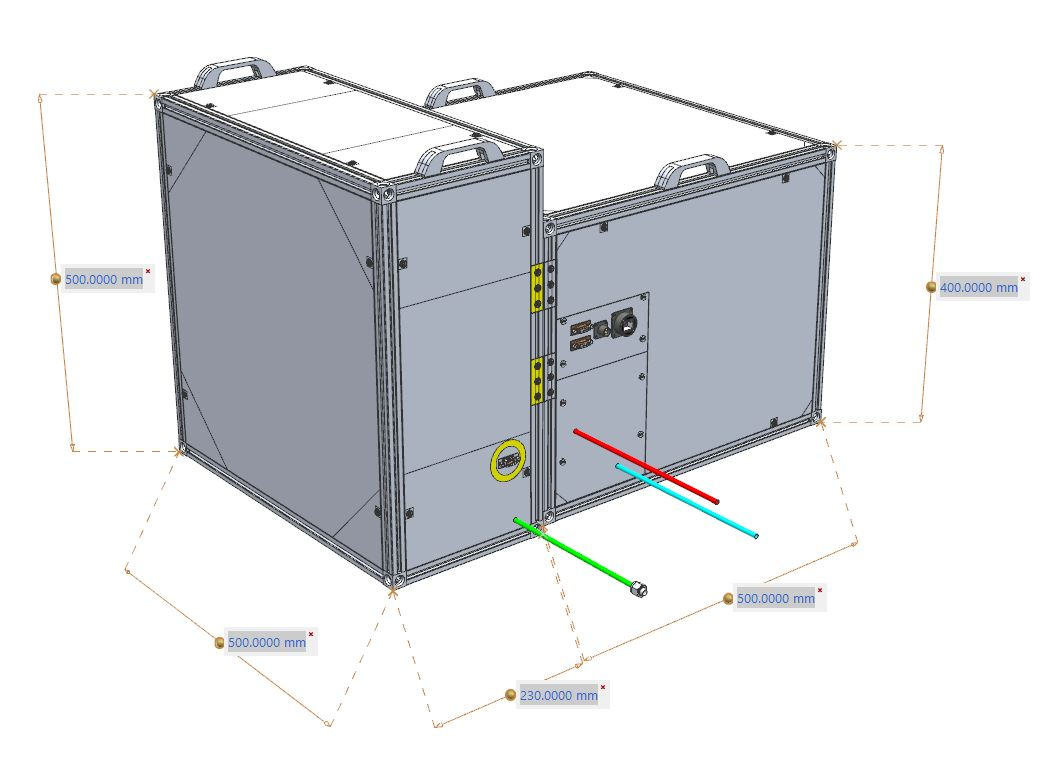
\includegraphics[width=0.9\textwidth]{4-experiment-design/img/Mechanical/tubular_dimensions.jpg}
     \caption{General Dimensions of the Experiment.}
     \label{dimensions}
\end{figure}

\begin{figure}[H]
    \centering
    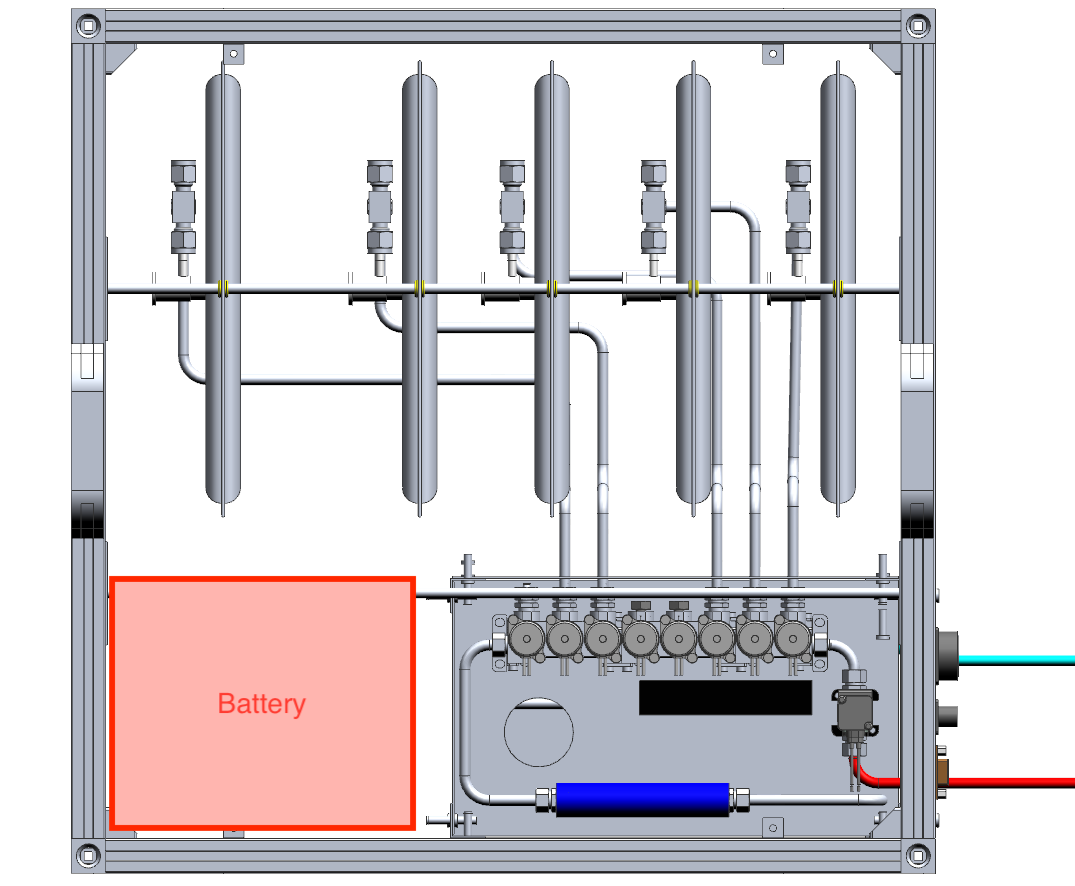
\includegraphics[width=0.45\textwidth]{4-experiment-design/img/Mechanical/Battery_Top_View.png}
    \caption{Layout Including a Battery (in Red).}
    \label{battery_distribution}
\end{figure}

The main mechanical characteristics of the experiment are summarized in Table \ref{table:experiment-summary}, where the values are based on the reference axis shown in Figure \ref{COG}. The Center Of Gravity for the whole experiment is determined to be located just on base of the third level of The Brain which coincides with the location of the electronics PCB. This outcome is quite advantageous in terms of stability for one of the most sensitive subsystems of the experiment in terms of shakes and loads. It should also be noted that the weights of the table for the boxes and, therefore, the whole experiment, are increased by a safety margin of $10\%$.

\begin{table}[H]
\noindent\makebox[\columnwidth]{%
\scalebox{0.8}{
\begin{tabular}{c|c|c|c|}
\cline{2-4}
 & CAC & AAC & TOTAL \\ \hline
\multicolumn{1}{|c|}{Experiment mass {[}kg{]}} & $12.08$ & $12.37$ & $24.45$ \\ \hline
\multicolumn{1}{|c|}{Experiment dimensions {[}m{]}} & $0.23\times0.5\times0.5$ & $0.5\times0.5\times0.4$ & $0.73\times0.5\times0.5$ \\ \hline
\multicolumn{1}{|c|}{Experiment footprint area {[}m^2{]}} & $0.115$ & $0.25$ & $0.365$ \\ \hline
\multicolumn{1}{|c|}{Experiment volume {[}m^3{]}} & $0.0575$ & $0.1$ & $0.1575$ \\ \hline
\multicolumn{1}{|c|}{Experiment expected COG position} & \begin{tabular}[c]{@{}l@{}}$X=23.51\ cm$\\ $Y=10\ cm$\\ $Z=22.57\ cm$ \end{tabular}  & \begin{tabular}[c]{@{}l@{}} $X=29.04\ cm$\\ $Y=16.63\ cm$\\  $Z=16.2\ cm$ \end{tabular} &\begin{tabular}[c]{@{}l@{}} $X=26.31\ cm$\\ $Y=24.99\ cm$\\  $Z=19.35\ cm$  \end{tabular} \\ \hline
\end{tabular}}}
\caption{Experiment Summary Table.}
\label{table:experiment-summary}
\end{table}


 \begin{figure}[H]
     \centering
     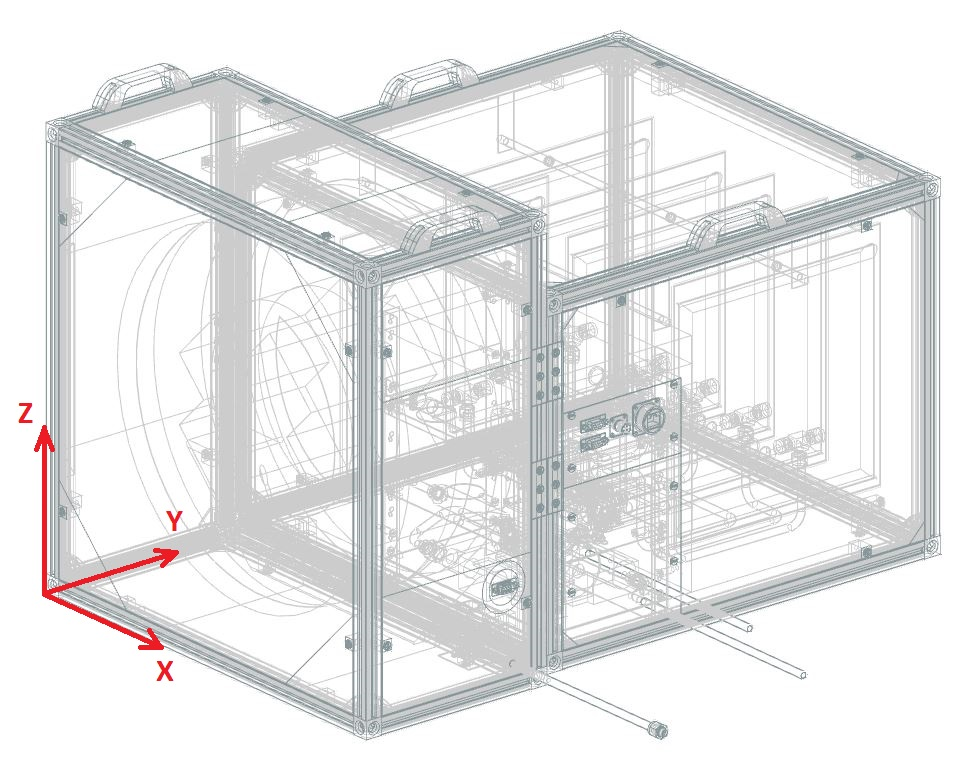
\includegraphics[width=0.45\textwidth]{4-experiment-design/img/Mechanical/COG.jpg}
     \caption{Reference Axis for the Total Center of Gravity.}
     \label{COG}
\end{figure}

\pagebreak
\subsubsection{Structure}
\label{sec:4.4.1}

The main purpose of an experiment box structure is to provide overall mechanical integrity and maintain the system geometry. It shall be able to carry the loads of all the phases of the flight and ensure that all the components and subsystems can withstand them. Test 9 in Table \ref{tab:vibration-test} will help to confirm the frame can withstand these vibrations and updates to the design will be made if necessary.

Moreover, other considerations such as electrical and, especially, thermal conductivity are also be a concern since the experiment will fly up to $25\ km$ in the Polar Circle in October and many critical subsystems have tight operative ranges values.

 \begin{figure}[H]
     \centering
     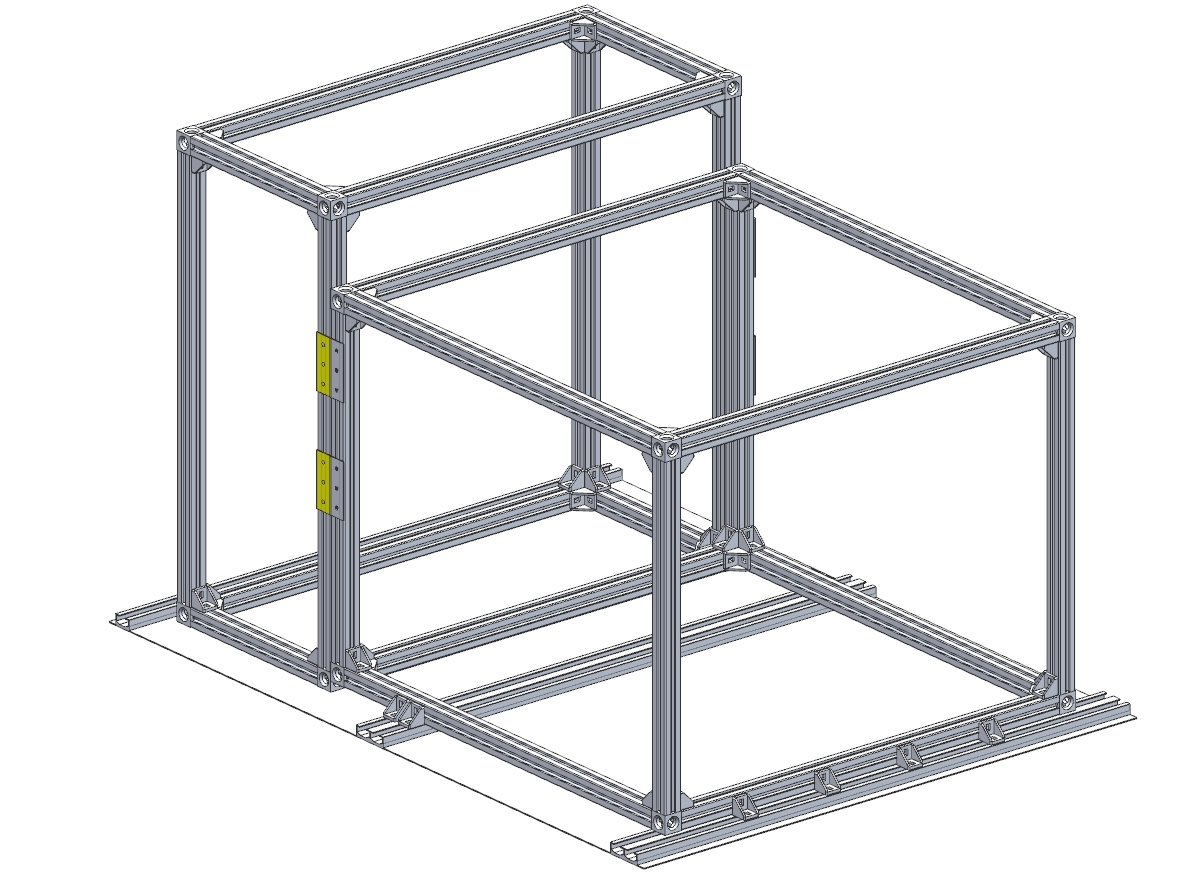
\includegraphics[width=0.8\textwidth]{4-experiment-design/img/Mechanical/structure_pic.jpg}
     \caption{Structure Overview.}
     \label{fig:structure}
\end{figure}

For this purpose, two boxes built with straight frames have been chosen as the best option as shown in Figure \ref{fig:structure}. The frame of these boxes will be strut profiles made of aluminum, with a characteristic cross-section of $20\times20\ mm$, and with $M6$ thread at each side. The rails will allow an easy interface between bars and other elements. In turn, these profiles will be joined together in each corner with aluminum cubic connectors of $20\times20\ mm$ (see Figure \ref{fig:corner_cube}) and $M6\times16$ bolts aligned with the bars axis. At the same time, these nodes will be reinforced by three $20/20$ brackets (see Figure \ref{fig:corner_bracket}) each that will be fixed to the frames with $M4\times8$ bolts and the corresponding $M4$ T-nut.

\bigskip
\begin{figure}[H]
    \noindent\makebox[\textwidth]{%
    \begin{subfigure}{.35\textwidth}
        \centering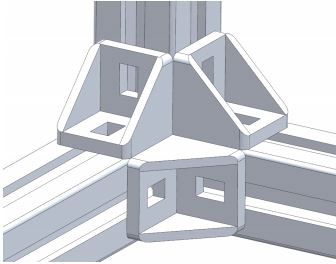
\includegraphics[width=1\textwidth]{4-experiment-design/img/Mechanical/corner_brackets.jpg}
        \caption{Brackets Reinforcement.}
        \label{fig:corner_bracket}
    \end{subfigure}
    \hspace{1cm}
    \begin{subfigure}{.35\textwidth}
        \centering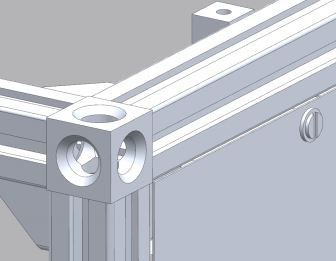
\includegraphics[width=1\textwidth] {4-experiment-design/img/Mechanical/corner_cube.jpg}
        \caption{Cubic Connector.}
        \label{fig:corner_cube}
    \end{subfigure}}
    \caption{Strut Profiles Connections.}
    \label{fig:profile_connection}
\end{figure}

\bigskip
Tables \ref{table:profile_material} and \ref{table:profile_momentum} below show the main mechanical properties of the Bosch Rexroth $20/20$ strut profiles used in the structure.


\begin{longtable}{|m{0.2\textwidth}|m{0.14\textwidth}|m{0.25\textwidth}|m{0.3\textwidth}|}
\hline
\textbf{Section surface} & \textbf{Mass} & \textbf{Moment of Inertia ($I_x = I_y$)} & \textbf{Moment of resistance ($W_x = W_y$)} \\ \hline 
$1.6\ cm^2$ & $0.4\ kg/m$ & $0.7\ cm^4$ & $0.7\ cm^3$ \\ \hline

\caption{Intrinsic Characteristics of the Strut Profiles.}
\label{table:profile_momentum}
\end{longtable}

\smallskip

\subsubsection{Walls and Protections}
\label{sec:4.4.2}

Since the experiment will be placed close to the outside of the gondola, it is very exposed to both external elements impacts and also possible broken parts from other experiments in the gondola due to unexpected rapid movements, and a probable hard landing impact. Therefore, the experiment box will be shielded with removable aluminum walls along with a thick layer of Styrofoam attached to each wall. This thickness varies from two to three centimeters in the AAC box, and five centimiters to protect the AirCore. Besides protection, the thickness of the styrofoam is also motivated by thermal control issues.
% which is explained more in detail in Section \ref{sec:4.6.6}.

To mount the experiment a combination of three different elements will be used, as shown in Figure \ref{fig:wall_attach}. The walls will be screwed to the Variofix blocks by means of $M4\times8$ bolts. In between the aluminum walls and the bolts, a $M4$ retainer ring will be placed to improve the fixation of each spot. Four fixation points for each wall have been considered sufficient to keep the experiment safe from any impact. However, double the amount of fixation points, eight, will be used in the more exposed walls that are facing outside the gondola.

The styrofoam sheets will be attached to the aluminum walls with polyamide washers screwed along both layers.

Tables \ref{table:wall_aluminum} and \ref{table:wall_styrofoam} show the main properties of the materials used to build the walls of the boxes.

 \begin{figure}[H]
     \centering
     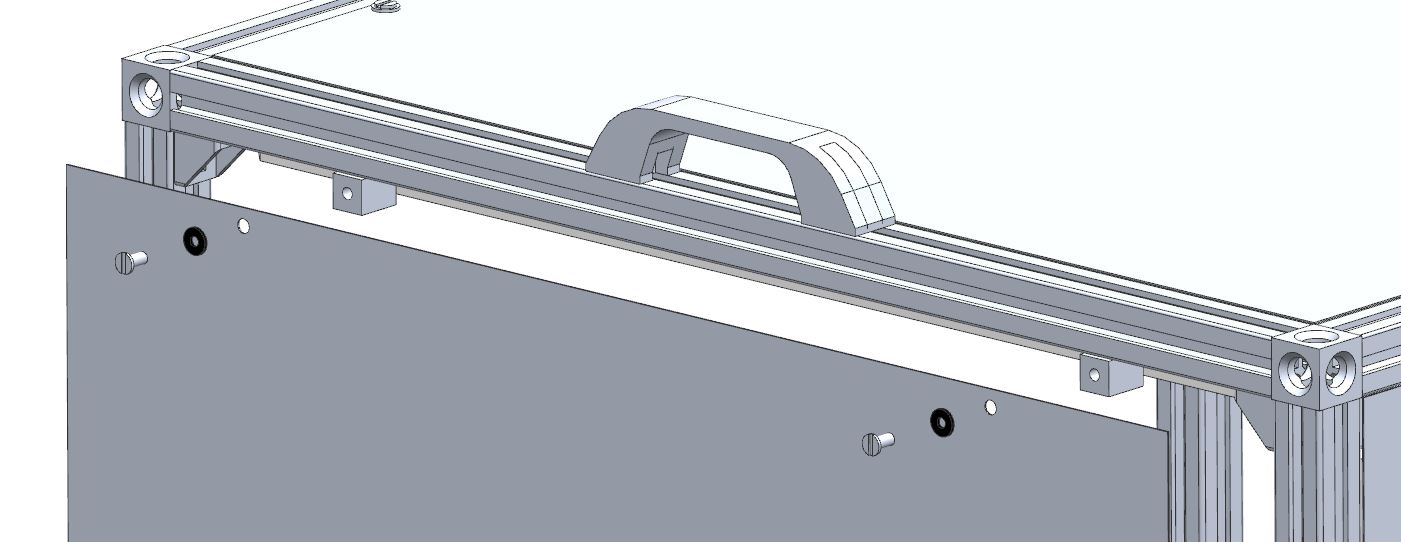
\includegraphics[width=0.8\textwidth]{4-experiment-design/img/Mechanical/wall_attachment.jpg}
     \caption{Exploit View of the Attachment of the Walls.}
     \label{fig:wall_attach}
\end{figure}

\subsubsection{CAC Box}

The CAC subsystem is designed to fit a $300$ m stainless steel coiled tube, a solenoid valve controlling it, interfaces, an air filter and three temperature sensors. A schematic of this subsystem can be seen in Figure \ref{fig:CAC-schematic}. The CAC consists of a combination of a $200$ m coiled tube of $1/8$ inches diameter and a $100$ m coiled tube of $1/4$ inches diameter. The outlet of the CAC is sealed with a quick connector provided by FMI. The inlet will be sealed the same way but it will be opened by another interface plugged into the quick connector. A filter is placed between this orifice and the solenoid valve. The filter will be custom made by FMI. The set up is a tube containing magnesium perchlorate powder with stone wool at both ends of the tube. It will ensure that no moisture will enter the coil during any testing or sampling. Another tube is attached to the solenoid valve that goes outside the box, thus having a direct outside outlet and inlet for the whole CAC system, as seen in Figure \ref{fig:CAC-cad-model}.

% mechanical issues and gondola constraints 

\begin{figure}[H]
    \centering
    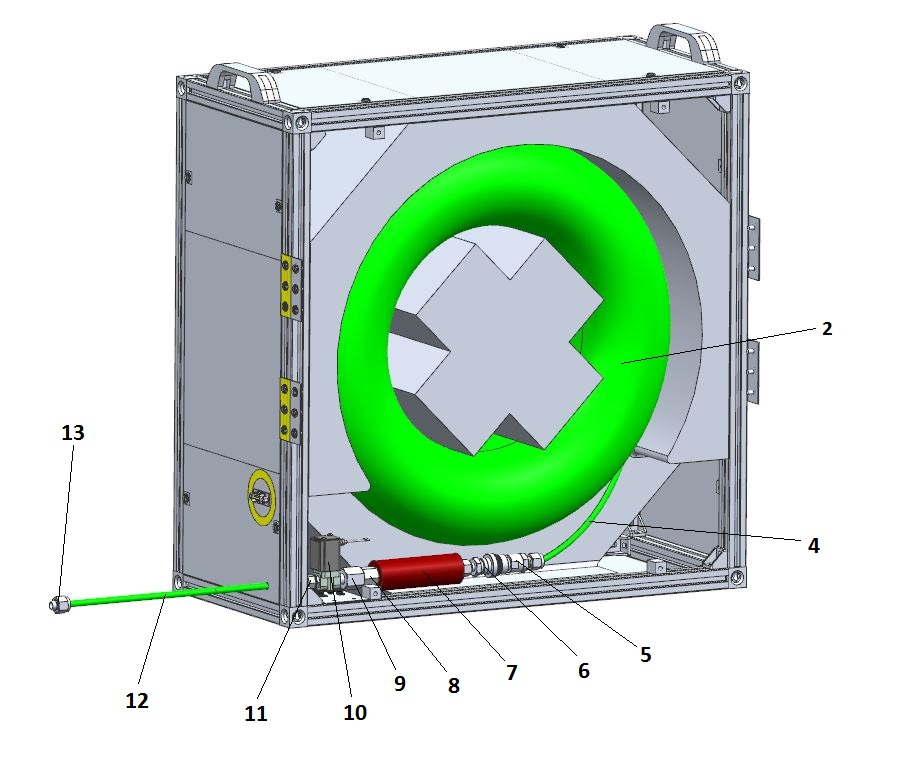
\includegraphics[width=0.7\textwidth]{4-experiment-design/img/Mechanical/CAC_interior_labels.jpg}
    \caption{3D Model of the CAC Box. The Numbers Correspond to the Numbers in Figure. \ref{fig:CAC-schematic}.}
    \label{fig:CAC-cad-model}
\end{figure}

\begin{figure}[H]
    \centering
    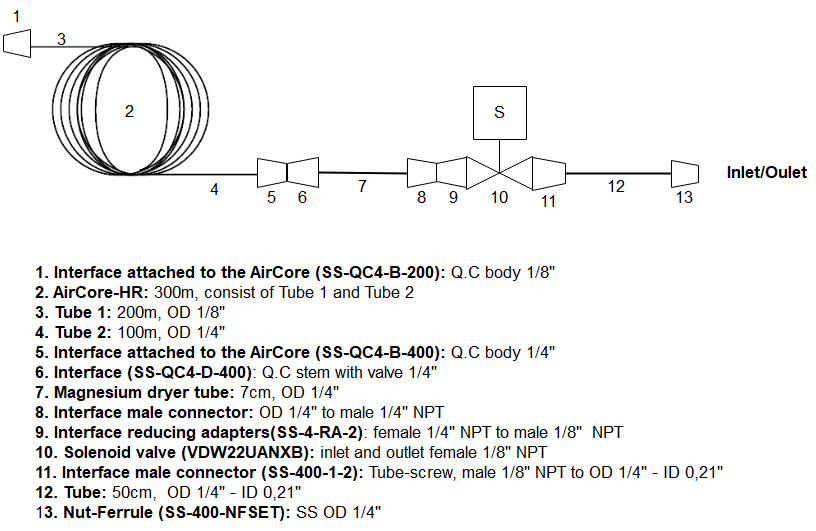
\includegraphics[width=1\textwidth]{4-experiment-design/img/Mechanical/CAC-schematic.PNG}
    \caption{Schematic of CAC.}
    \label{fig:CAC-schematic}
\end{figure}
\smallskip
The electronic components in the CAC box will be: three temperature sensors and the solenoid valve. In order to connect these components to the control unit in the AAC box, a D-sub cable will link the respective D-sub connector on each box.

\subsubsection{AAC Box}\label{sec:aac-analysis}
The AAC box has been designed to be as compact as possible. An analysis regarding the variation of the bags dimensions to different sampled volume, has been made and summarized in Appendix \ref{dimensions-bags}. From these results it was shown that the AAC subsystem is able to fit six $3\ L$ sampling bags together The Brain that includes the pneumatic system and the electronic box. Each bag will have a dedicated valve in the Valve Center (VC) to allow emptying and filling processes as well as to close the bag when needed. The bags will be hanging from a bar that will be attached to the structure frame by two anchor points on the top. The distribution layout can be seen in Figures \ref{iso_aac} and \ref{lateral_aac}. 


%The AAC Subsystem consists of six $3\ L$ sampling bags. Each bag will have a dedicated valve in the Valve Center (VC) to allow emptying and filling processes as well as to close the bag when needed. The bags will be placed vertically and will have two anchor points: on the top through a  multiple anchor interface (see Figure \ref{anchor_bags}) and on the bottom by means of the tubes connecting them to the valves.

%% Several Figures of the top box with its inside elements: isometric, top view and front view.

%\begin{figure}[H]
%    \centering
%    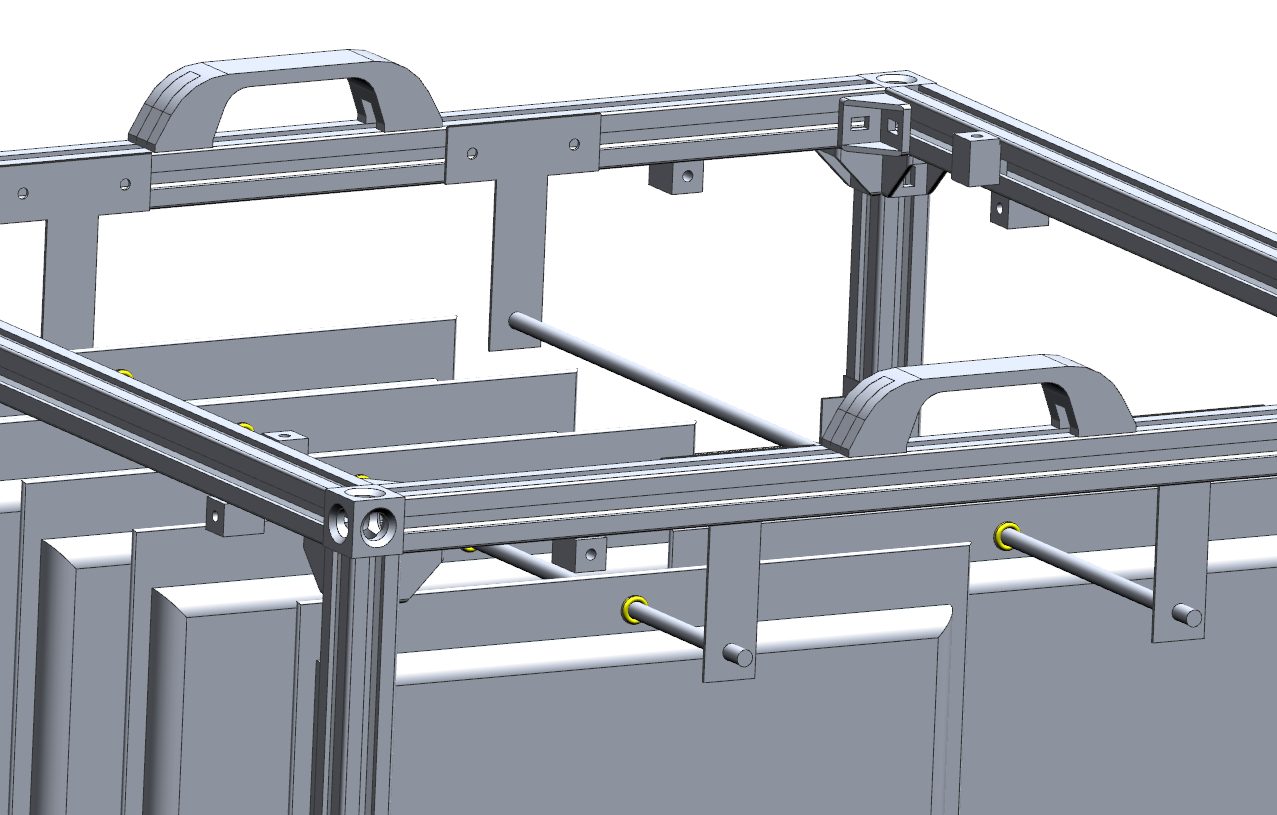
\includegraphics[width=0.6\textwidth]{4-experiment-design/img/Mechanical/Bags_Fixing_Interface.png}
%    \caption{Sampling Bags with Fixing Interface and the AAC Box Handles.}
%    \label{anchor_bags}
%\end{figure}


%\underline{Distribution}

%The AAC box has been designed to be as compact as possible, which was a challenging iterative process since the bags dimensions vary during the flight. The process led to a square base box that is able to fit six sampling bags together with a control center called The Brain that includes the pneumatic system and the electronic box. The distribution layout can be seen in Figures \ref{iso_aac} and \ref{lateral_aac}.

% Figure: Top view to show the distribution of the AAC Box

\begin{figure}[H]
    \centering
    \begin{subfigure}[b]{0.47\textwidth}
        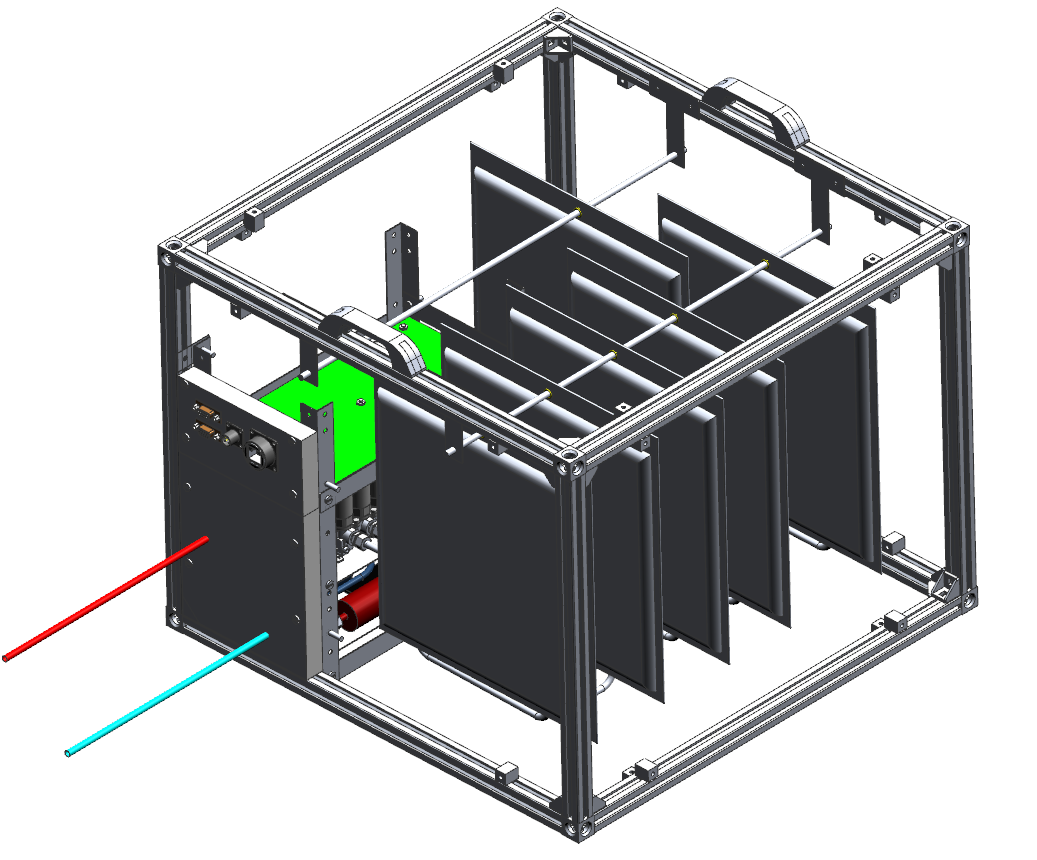
\includegraphics[width=\textwidth]{4-experiment-design/img/Mechanical/AAC_isometric_view.png}
         \caption{Isometric View of the AAC Box.}
    \label{iso_aac}
    \end{subfigure}
    ~
    \begin{subfigure}[b]{0.47\textwidth}
        \centering
         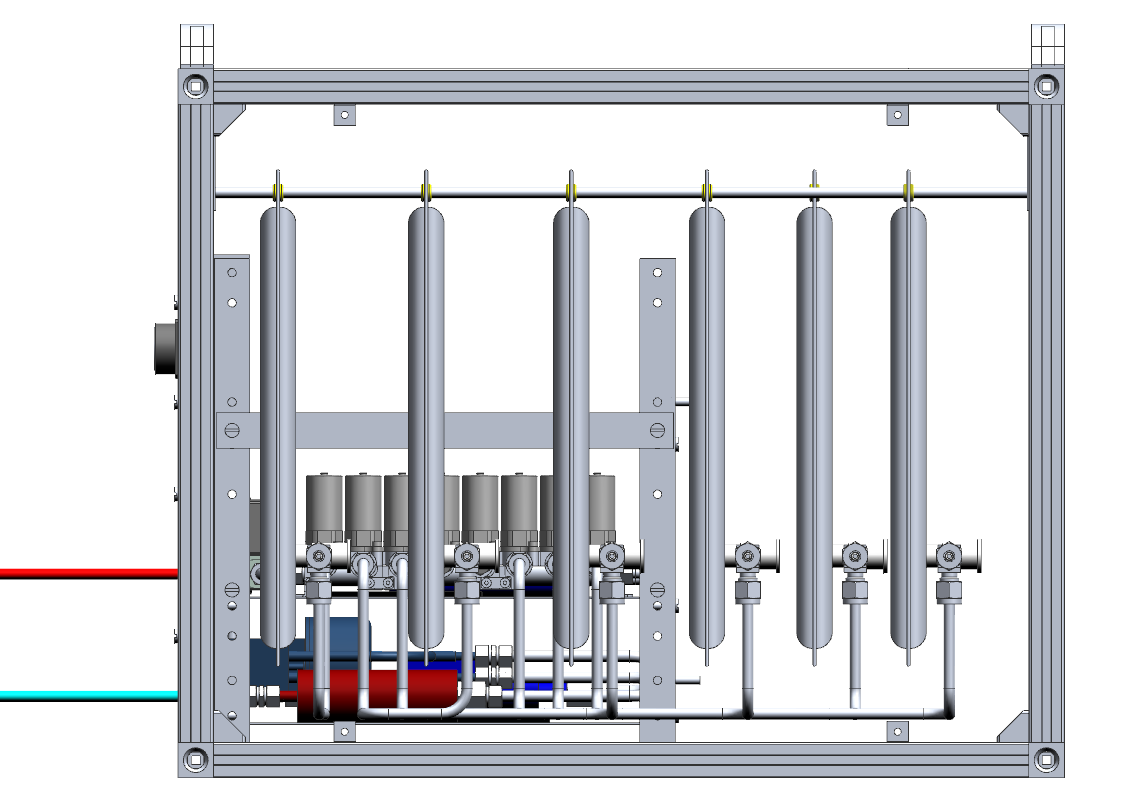
\includegraphics[width=\textwidth]{4-experiment-design/img/Mechanical/AAC_lateral_view.png}
        \caption{Lateral View of the AAC Box.}
        \label{lateral_aac}
        \end{subfigure}
    \caption{Distribution Inside the AAC Box.}
    \label{fig:Distribution-AAC}
\end{figure}

%\begin{figure}[H]
%    \centering
%    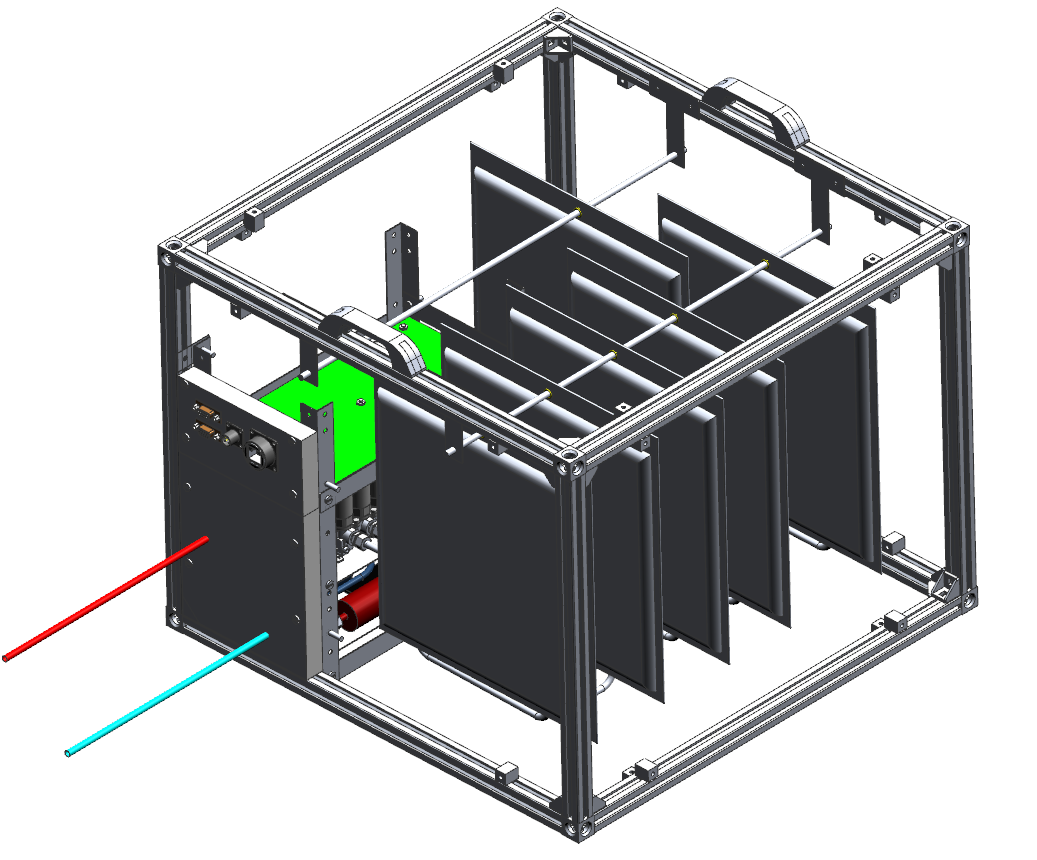
\includegraphics[width=0.6\textwidth]{4-experiment-design/img/Mechanical/AAC_isometric_view.png}
%    \caption{Isometric View of the AAC Box.}
%    \label{iso_aac}
%\end{figure}

%%\begin{figure}[H]
%    \centering
%    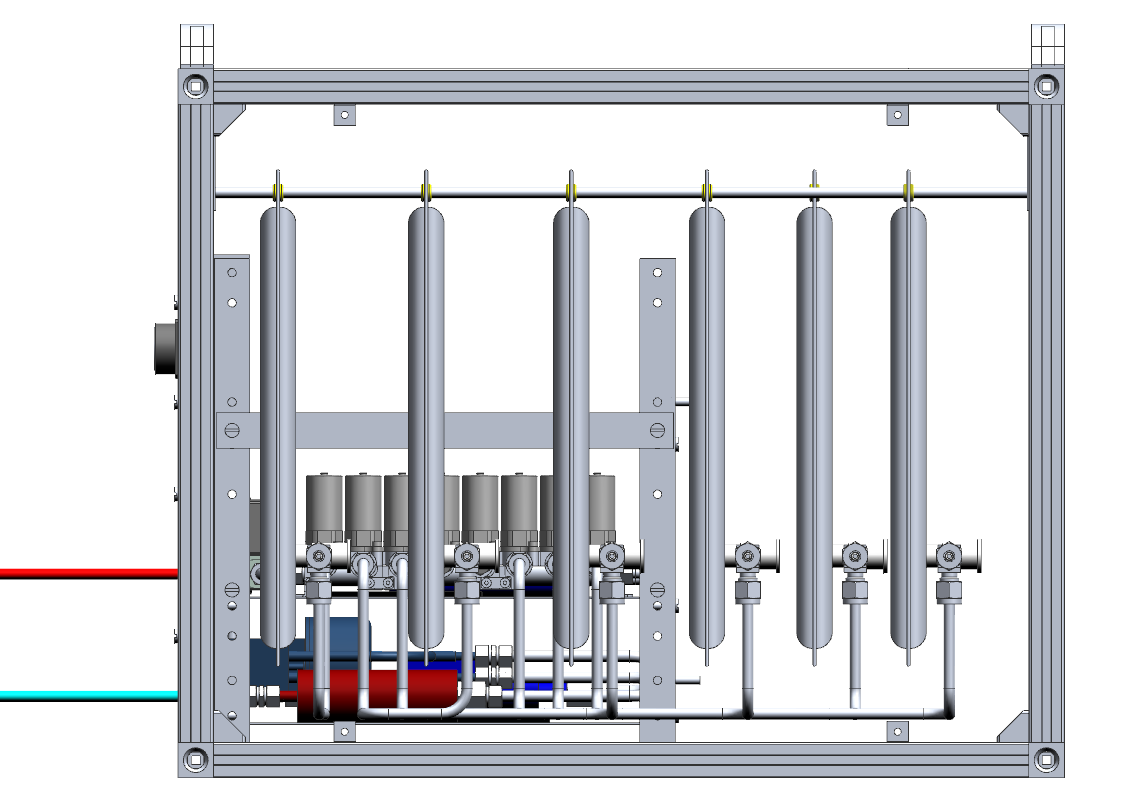
\includegraphics[width=0.6\textwidth]{4-experiment-design/img/Mechanical/AAC_lateral_view.png}
%    \caption{Lateral View of the AAC Box.}
%    \label{lateral_aac}
%\end{figure}

%\begin{figure}[H]
%    \centering
%    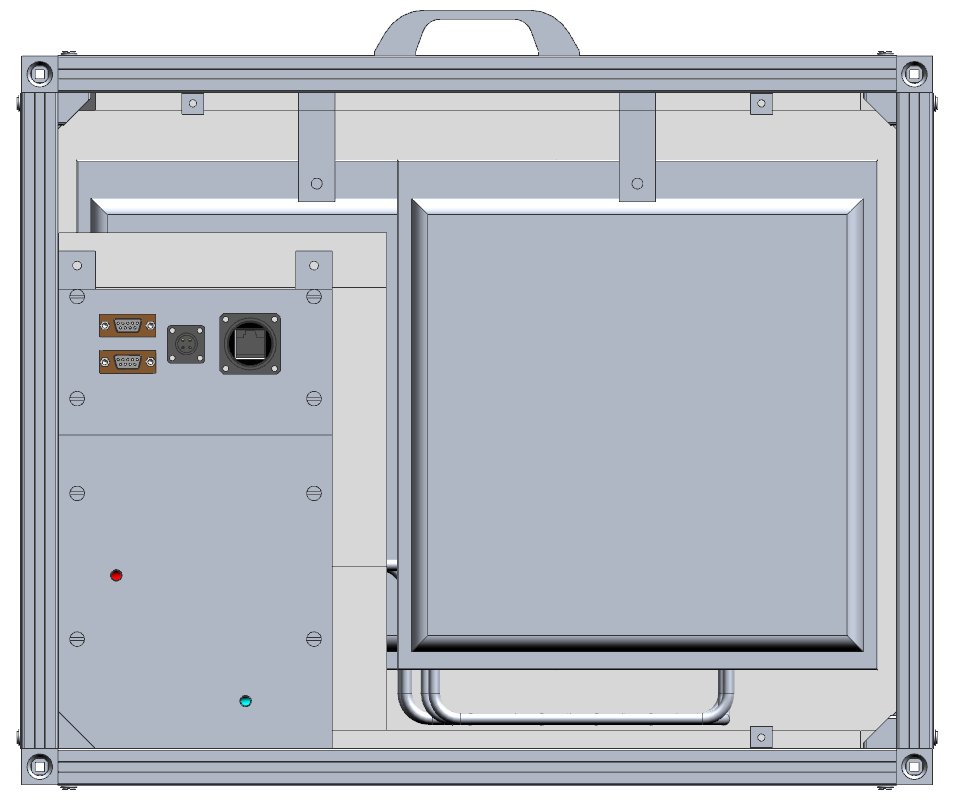
\includegraphics[width=0.7\textwidth]{4-experiment-design/img/Mechanical/AAC_front_view.png}
%    \caption{Front View of the AAC Box.}
%    \label{front_aac}
%\end{figure}
In order to reach to all the bags from the Valve Center, the tubes are brought to the base of the box. More detail on its positioning is included in the following section. 
%Since the AAC box is expected to be handed over to FMI, the design also takes into consideration the possibility to include a battery for power supply. This would be allocated next to The Brain and imply reducing the sampling bags down to five, see Figure \ref{battery_distribution}.

% Figure with a a top view without the 6th bag and with a red box simulating the battery

\bigskip
\underline{The Brain}
\label{subsec:brain}

\smallskip
The Brain is an essential part of the experiment. It is a three-level structure containing both the pneumatic system and the electronics of the experiment, seen in Figure \ref{brain_isometric_open}. Its design aimed to make it compact enough to both allow a proper thermal control and to fit into the space left next to the sampling bags. It is placed in a corner of the AAC box. Therefore, The Brain takes advantage of the vertical space inside the AAC box. It has three different levels: Level 1 - Pump, Level 2 - Valve Center and Level 3 - Electronics.


\begin{figure}[H]
    \centering
    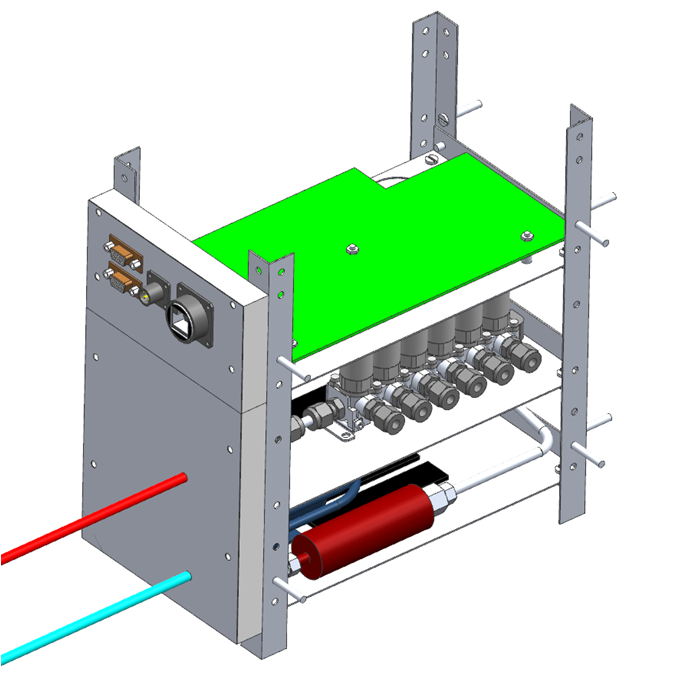
\includegraphics[width=0.43\textwidth]{4-experiment-design/img/Mechanical/The_Brain_Isometric.png}
    \caption{\DIFdelbeginFL \DIFdelFL{Isometric View }\DIFdelendFL \DIFaddbeginFL \DIFaddFL{Inside view }\DIFaddendFL of The Brain.}
    \label{brain_isometric_open}
\end{figure}
Level 1 of The Brain is lying on the base wall styrofoam. It contains the beginning of the pneumatic sampling system. The inlet tube passes through the wall and interfaces with the filter. From here the system continues through the pump, airflow sensor and to Level 2. The reason for having the pump in Level 1 is to have the minimum vibration transmitted to the other components. The pump will have two heaters close by that will be used to regulate its temperature. This can be seen as two black rectangular sheets underneath the pump in Figure \ref{level_1}.

The second level of The Brain is responsible for the distribution of the air to the selected sampling bag. The manifold with 8 solenoid valves is the main component. From here, the tubes connect with the bags. A T-Union connection is used just before the bag valve. This interface allows the pre-flight flushing of the tubes connecting with the valves as explained previously. 

\smallskip
The flushing valve is the responsible to ensure a proper flushing of the system before each sampling period. From the flushing valve, a outlet tube (in red) reaches the outside environment. This can be seen in Figure \ref{level_2}.

The OBC and its external elements will be allocated in the third level of The Brain. The PCB will be fixed to the aluminum plate by means of 5 standoffs. As shown in Figure \ref{level_3}, it has a hole, as well as the level plate, to collect all the wires connecting with levels 1 and 2. This level has its own outside wall which contains the electrical interfaces. The latter allows to open the wall without having to remove all the sockets attached with screws and a female in the inside of the wall. The styrofoam shielding of The Brain has a hole at this height to allow the temperature sensors wires to reach the inside of the AAC Box. 

A more detailed content of the components for each level is summarized in Appendix \ref{list-of-components-brain}.
\begin{figure}[H]
    \centering
    \begin{subfigure}[b]{0.3\textwidth}
    \centering
    \includegraphics[width=\textwidth]{4-experiment-design/img/Mechanical/Level_1.png}
    \caption{Isometric View of Level 1.}
    \label{level_1}
    \end{subfigure}
    ~
    \begin{subfigure}[b]{0.3\textwidth}
    \centering
    \includegraphics[width=\textwidth]{4-experiment-design/img/Mechanical/Level_2.png}
    \caption{Isometric View of Level 2.}
    \label{level_2}
    \end{subfigure}
    ~
    \begin{subfigure}[b]{0.3\textwidth}
    \centering
    \includegraphics[width=\textwidth]{4-experiment-design/img/Mechanical/Level_3.png}
    \caption{Isometric View of Level 3.}
    \label{level_3}
    \end{subfigure}
    \caption{Distribution in Each Level.}
    \label{fig:The-brain}
\end{figure}
%Level 1 is the base of the AAC box and together with Level 2 contain the main pneumatic system. This is commanded by the electronics in the top level. This distribution allows easy access to the PCB from the top and provides the physical desired separation between electronics and pneumatic circuit. 

This distribution allows easy access to the PCB from the bottom and provides the physical desired separation between electronics and pneumatic circuit.
%This is shown in the dedicated section for each level which can be seen in Figure \ref{brain_lateral}.

%\begin{figure}[H]
%    \centering
%    \includegraphics[width=0.6\textwidth]{4-experiment-design/img/Mechanical/Brain_Lateral.png}
%    \caption{Lateral View of The Brain.}
%    \label{brain_lateral}
%\end{figure}

\smallskip
The structure of The Brain provides versatility in terms of implementation and construction. It is made out of four aluminum 90-degree angle bars \DIFdelbegin \DIFdel{and five flat bars to join them together}\DIFdelend \DIFaddbegin \DIFadd{placed vertically and six aluminum 90-degree angle bars placed horizontally, 2 on each level}\DIFaddend . The bars have custom-made holes that allow the \DIFdelbegin \DIFdel{1 mm thick aluminum plate of each level to be fixed by means of two bolts on each column, one over and one below it. They allow the possibility }\DIFdelend \DIFaddbegin \DIFadd{possibility to fix all the pieces together and }\DIFaddend to provide the anchor point for the lateral and top styrofoam shield as well as to fix the whole unit to the box structure bars. \DIFdelbegin \DIFdel{This is seen in Figure \ref{brain_structure}. 
}\DIFdelend %DIF > This is seen in Figure \ref{brain_structure}. 

\DIFdelbegin %DIFDELCMD < \begin{figure}[H]
%DIFDELCMD <     \centering
%DIFDELCMD <     \begin{subfigure}[b]{0.48\textwidth}
%DIFDELCMD <     \centering
%DIFDELCMD <     \includegraphics[width=\textwidth]{4-experiment-design/img/Mechanical/Brain_Structure.png}
%DIFDELCMD <     %%%
%DIFDELCMD < \caption{%
{%DIFAUXCMD
\DIFdelFL{Structure of The Brain.}}
    %DIFAUXCMD
%DIFDELCMD < \label{brain_structure}
%DIFDELCMD <     \end{subfigure}
%DIFDELCMD <     %%%
\DIFdelFL{~
    }%DIFDELCMD < \begin{subfigure}[b]{0.48\textwidth}
%DIFDELCMD <     \centering
%DIFDELCMD <     \includegraphics[width=\textwidth]{4-experiment-design/img/Mechanical/Brain_Isometric.png}
%DIFDELCMD <     %%%
%DIFDELCMD < \caption{%
{%DIFAUXCMD
\DIFdelFL{Isometric View of The Brain with Walls.}}
    %DIFAUXCMD
%DIFDELCMD < \label{brain_isometric}
%DIFDELCMD <     \end{subfigure}
%DIFDELCMD <     %%%
%DIFDELCMD < \caption{%
{%DIFAUXCMD
\DIFdelFL{Design of The Brain.}}
    %DIFAUXCMD
%DIFDELCMD < \label{fig:The-brain}
%DIFDELCMD < \end{figure}
%DIFDELCMD < %%%
\DIFdelend %DIF >  \begin{figure}[H]
%DIF >      \centering
%DIF >      \begin{subfigure}[b]{0.48\textwidth}
%DIF >      \centering
%DIF >      \includegraphics[width=\textwidth]{4-experiment-design/img/Mechanical/Brain_Structure.png}
%DIF >      \caption{Structure of The Brain.}
%DIF >      \label{brain_structure}
%DIF >      \end{subfigure}
%DIF >      ~
%DIF >      \begin{subfigure}[b]{0.48\textwidth}
%DIF >      \centering
%DIF >      \includegraphics[width=\textwidth]{4-experiment-design/img/Mechanical/Brain_Isometric.png}
%DIF >      \caption{Isometric View of The Brain with Walls.}
%DIF >      \label{brain_isometric}
%DIF >      \end{subfigure}
%DIF >      \caption{Design of The Brain.}
%DIF >      \label{fig:The-brain}
%DIF >  \end{figure}



%\begin{figure}[H]
%    \centering
%    \includegraphics[width=0.8\textwidth]{4-experiment-design/img/Mechanical/Brain_Structure.png}
%    \caption{Structure of The Brain.}
%    \label{brain_structure}
%\end{figure}

\smallskip
The bulk dimensions of The Brain are 260 mm long, 150mm wide and 290 mm high. If the shielding styrofoam walls are taken into account, the dimensions are 290 mm long, 180 mm wide and 300 mm high.
Therefore, accounting for the space the column bars take, each plate has a surface of 258 mm x 158 mm. The distance between levels is variable depending on the components dimensions. Level 1 has a height if 7 cm, Level 2 has a height of 9 cm and Level 3 has 8 cm to the top styrofoam shielding. The Brain with styrofoam \DIFdelbegin \DIFdel{sheilding }\DIFdelend \DIFaddbegin \DIFadd{shielding }\DIFaddend can be seen in Figure \ref{brain_isometric}.

%DIF < \begin{figure}[H]
%DIF <     \centering
%DIF <     \includegraphics[width=0.8\textwidth]{4-experiment-design/img/Mechanical/Brain_Isometric.png}
%DIF <     \caption{Isometric View of The Brain.}
%DIF <     \label{brain_isometric}
%DIF < \end{figure}
\DIFaddbegin \begin{figure}[H]
    \centering
    \includegraphics[width=0.8\textwidth]{4-experiment-design/img/Mechanical/Brain_Isometric.png}
    \caption{\DIFaddFL{Isometric view of The Brain.}}
    \label{brain_isometric}
\end{figure}
\DIFaddend 

\smallskip
In order to allocate the electrical interfaces required (E-Link, Power Supply and D-Sub Connectors) as well as to allow the tubes of the sampling system to reach the outside environment, the outside facing wall is divided in three pieces. Two small pieces of \DIFdelbegin \DIFdel{aluminium }\DIFdelend \DIFaddbegin \DIFadd{aluminum }\DIFaddend sheet are fixed to The Brain structure, as seen in Figure \ref{brain_isometric}. This will make it easy to manipulate when having to open the box wall since the little pieces containing the interfaces and the tubes holes, will remain attached. The bottom piece covers Level 1 and 2 while the other, which contains the electrical connections, protects Level 3. These pieces have the same layout as the main wall. 
\DIFaddbegin \DIFadd{Since the electrical panel is facing to the outside, to avoid any interference with the gondola, the experiment has to be fixed inside it at a certain distance with a safe margin. If the latter is not possible, the whole experiment should then be twisted 180 degrees so the panels would face inwards. Then, the pipes will have to be longer in order to reach the outside of the gondola for clear air samples. 
}\DIFaddend 





%\begin{figure}[H]
%    \centering
%    \includegraphics[width=0.8\textwidth]{4-experiment-design/img/Mechanical/Level_1.png}
%    \caption{Isometric View of Level 1.}
%    \label{level_1}
%\end{figure}


%\begin{figure}[H]
%    \centering
%    \includegraphics[width=0.8\textwidth]{4-experiment-design/img/Mechanical/Level_2.png}
%    \caption{Isometric View of Level 2.}
%    \label{level_2}
%\end{figure}



%\begin{figure}[H]
%    \centering
%    \includegraphics[width=0.8\textwidth]{4-experiment-design/img/Mechanical/Level_3.png}
%    \caption{Isometric View of Level 3.}
%    \label{level_3}
%\end{figure}

\bigskip
\underline{Shielding and anchor points}

\smallskip
The most critical components in terms of required thermal control are inside The Brain. These are the pump and the valves. In order to provide a passive thermal shielding, 3 cm thick removable styrofoam walls are placed in the three walls (top and laterals) facing the interior of the AAC box, shown in Figure \ref{brain_isometric}. The lateral walls are fixed by means of four bolts attached to the structure bars that penetrate inside the styrofoam. The top wall is fixed in place taking advantage of the structure columns which penetrate inside it. The larger lateral wall, where the tubes from the valves are, is divided in two pieces so it can be removed without having to disconnect the tubes. 

\smallskip
The Brain is fixed to the structure of the AAC box by means of \DIFdelbegin \DIFdel{two anchor points}\DIFdelend \DIFaddbegin \DIFadd{four anchor points: two flat plates and two 90-degree angles}\DIFaddend . In order to keep it in its place, the structure bars penetrate 3 cm into the styrofoam base.

%\begin{figure}[H]
%    \centering
%    \includegraphics[width=1\textwidth]{4-experiment-design/img/Mechanical%/Panel_Front.png}
%    \caption{Front View of The Brain Where the Styrofoam Walls can be Identified.}
%    \label{brain_front}
%\end{figure}

\subsubsection{Pneumatic Subsystem}
\label{sec:4.4.5}

In order to be able to collect separated samples of air, a pneumatic subsystem has been developed. The schematics and components of this can be seen in Figure \ref{pneumatic_system}. The system is formed by almost $100$ components located inside The Brain and the AAC Box. 

In between these components, the same Sulfinert-treated stainless steel tubing as the ones used for the Inlet/Outlet pipes explained in Section \ref{subsec:pipes} have been chosen. According to the datasheet, the minimum suggested bend radius for the chosen diameter tube is $10.2\ cm$. Any bend sharper than this may cause the tubing to stretch, potentially creating active sites as the coating layer density decreases. For this reason, \DIFdelbegin \DIFdel{an auxiliary }\DIFdelend $90^\circ$ elbow \DIFdelbegin \DIFdel{interface has been added }\DIFdelend \DIFaddbegin \DIFadd{interfaces have been used instead of the previously considered straight ones,  }\DIFaddend to perform all the required sharp curves to allocate all the components inside the volume-limited \emph{Brain}.

The schematic for the pneumatic system can be seen in Figure \ref{pneumatic_system}. The air is sucked from the outside through the inlet tube (No.1), turquoise in Figure \ref{pneumatic_system_cad}, and it goes through the filter (No.3) inside the pump (No.7). From here, it passes through the airflow sensor (No.11), which allows to monitor the flow rate, before changing to Level 2. Thereafter the air passes through the \DIFdelbegin \DIFdel{sensor box }\DIFdelend \DIFaddbegin \DIFadd{static pressure sensor }\DIFaddend (No.15) \DIFdelbegin \DIFdel{which contains three pressure sensors }\DIFdelend before getting to the six stations manifold (No.19). It is in here where the air is directed to the desired bag (No.31) thanks to its dedicated solenoid valve (No.26).

When flushing the pneumatic system before each sampling period, the flushing valve (No.23) is opened so that the outlet of the system is open and new air runs through the main part of the pneumatic system. 

%\begin{figure}[H]
%    \centering
%    \begin{subfigure}[b]{0.48\textwidth}
%    \centering
%    \includegraphics[width=\textwidth]{4-experiment-design/img/Mechanical/ Pneumatic_System_Top_View_Level_1.png}
%    \caption{Top View of Level 1.}
%    \label{level_1_pneumatic_system_top_view}
%    \end{subfigure}
%    ~
%    \begin{subfigure}[b]{0.48\textwidth}
%    \centering
%    \includegraphics[width=\textwidth]{4-experiment-design/img/Mechanical/Pneumatic_System_Top_View_Level_2.png}
%    \caption{Top View of Level 2.}
%    \label{level_2_pneumatic_system_top_view}
%    \end{subfigure}
%    \caption{View Over the Pneumatic System.}
%    \label{fig:Pneumatic-system}
%\end{figure}

\begin{figure}[H]
    \centering
   \DIFdelbeginFL %DIFDELCMD < \includegraphics[width=0.8\textwidth]{4-experiment-design/img/Mechanical/Pneumatic_System.png}
%DIFDELCMD <    %%%
\DIFdelendFL \DIFaddbeginFL \includegraphics[width=0.43\textwidth]{4-experiment-design/img/Mechanical/Pneumatic_System.png}
   \DIFaddendFL \caption{Pneumatic System \DIFdelbeginFL \DIFdelFL{Top View}\DIFdelendFL \DIFaddbeginFL \DIFaddFL{top view}\DIFaddendFL .}
    \label{pneumatic_system_cad}
\end{figure}

%\begin{figure}[H]
%    \centering
%    \includegraphics[width=0.8\textwidth]{4-experiment-design/img/Mechanical/Pneumatic_System_Top_View_Level_2.png}
%    \caption{Pneumatic System Top View of Level 2.}
%    \label{level_2_pneumatic_system_top_view}
%\end{figure}

% Figure with the diagram

\newpage
\begin{landscape}
\begin{figure}[H]
    \centering
    \includegraphics[width=1.45\textwidth]{4-experiment-design/img/Mechanical/AAC_Subsystem.png}
    \caption{AAC Pneumatic System \DIFdelbeginFL \DIFdelFL{Diagram }\DIFdelendFL \DIFaddbeginFL \DIFaddFL{diagram }\DIFaddendFL and \DIFdelbeginFL \DIFdelFL{Components}\DIFdelendFL \DIFaddbeginFL \DIFaddFL{components}\DIFaddendFL .}
    \label{pneumatic_system}
\end{figure}
\end{landscape}

\raggedbottom
\pagebreak
\subsection{Electrical Design}

\subsubsection{Block Diagram}
\label{sec:4.5.1}

The electronics design can be seen in Figure \ref{fig:electronics-block-diagram} which shows the connections, grounding, voltages, and signals. 

\begin{figure}[H]
    \begin{align*}
        \includegraphics[width=16cm]{block-diagram-2.png}
    \end{align*}
    \caption{Block Diagram for all Electronic Components Showing the Connection, Signal and Power Connections.}\label{fig:electronics-block-diagram}
\end{figure}

Most of the electronics will be located in the Brain inside the AAC box. However, there will be six distinct areas:

\begin{enumerate}
    \item The Brain level 3, where the PCB is located with the Arudino and shield, two 24 V DC-DC, two 12 V DC-DC, one temperature sensor, 11 MOSFETs and 16 LEDs.
    \item The Brain level 2, where the valve manifolds with six sampling valves, the flushing valve, two heaters and one temperature sensor are located.
    \item The Brain level 1, where the pump, two heaters, airflow sensor, one temperature sensor and \DIFdelbegin \DIFdel{an inline }\DIFdelend \DIFaddbegin \DIFadd{static }\DIFaddend pressure sensor are located.
    \item The AAC box, where 3 ambient temperature sensors are located.
    \item The CAC box, where the CAC valve and 3 ambient temperature sensors are located.
    \item Outside of the experiment box, where 3 ambient pressure sensors are located.
\end{enumerate}

From the PCB, on level 3, five D-sub connectors will be used to connect to the other five areas. A 25 pin connector will be used for level 1, 15 pin connector will be used for level 2 and nine pin connectors will be used for the CAC box, AAC box sampling bags area, and the external pressure sensors. In addition there will be a connection to the gondola power and gondola E-link.

All of the power distribution will take place on the PCB using two 24 V DC-DC and two 12 V DC-DC converters in parallel with a forwarding diode.  
\begin{itemize}
  \item $28.8 \, V \Longrightarrow 24 \, V $ By DC-DC converters
  \item $28.8 \, V \Longrightarrow 12 \, V$ By DC-DC converters
  \end{itemize}
The heaters will not require the voltage to be stepped down and so will be powered directly from the gondola battery.

The Arduino will control all of the sensors, valves, heaters and the pump from the PCB. Sensors will be directly connected to the Arduino. The valves, heaters and the pump will be connected via a switching circuit.

The LEDs are used as visual indicators that display whether different parts of the circuit are alive or not. They give indications on the status of the valves, pump, heaters, DC-DC converters and Arduino. 

Grounding will be following a distributed single point grounding, with all ground connections meeting at a single star point to ensure there are no floating grounds. As not all components are connected via DC-DC converters the experiment will not be isolated from the gondola power supply therefore there will be a connection between the star point and the gondola ground. The star point will be located on the main PCB board which will then be grounded to the experiment box. The grounding can be seen in Figure \ref{fig:electronics-block-diagram} where it is indicated by dashed lines labeled GND. The analog sensors that are used on level 1 in the brain use a separate grounding wire(AGND) onto the main PCB where there is a separate trace connecting to the ground pins on the Arduino board. Furthermore the upper and lower level of the main PCB board will make use of one common grounding plane.

\subsubsection{Miniature Diaphragm Air Pump}
The pump which has been selected is the 850.1.2. KNDC B, Figure \ref{fig:pumppic}, which is manufactured by KNF. One of the reasons this pump has been selected is that it has successfully been flown on a similar flight in the past where it managed to pump enough air at 25 km altitude to have 180 mL remaining at sea level \cite{LISA}. However, to ensure the pump will operate as intended, several tests will still be carried out. These tests --- 4, 5, 18, 28 and 29, can be seen in Tables \ref{tab:vacuum-test}, \ref{tab:thermal-test}, \ref{tab:pump-low-pressure-test}, \ref{tab:pump-operation-test}, and \ref{tab:pump-current-pressure-test}. The pump has already passed three of these tests and their results can be seen in Section \ref{sec:test28result} for Test 28, Section \ref{subsection:pumplowpressuretest} for Test 18 and Section \ref{sec:test29result} for Test 29.

At sea level conditions the pump was tested and found to have a flow rate of 8.0 L/min and a current draw of 250 mA. The peak current draw was recorded as 600 mA which lasts for less than one second and occurs when the pump is switched on. 

From the results of Test 18, in Section \ref{subsection:pumplowpressuretest}, the flow rate is estimated to be 3.0 L/min at the lowest pressure that will be seen in flight. This is in line with requirement D23. The results found in Test 28, in Section \ref{sec:test28result}, appear to be inline with the information given by the manufacturer, seen in Figure \ref{fig:pumpflowcur}.  The highest continuous current draw expected from the pump is 185 mA when the experiment is at 12 km altitude and is expected to decrease as we increase in altitude. While it appears the pump increases in current draw at around 6 km there is no plan to sample below 12 km therefore the highest current draw can be taken from 12 km. As the pump has a peak current of 600 mA when it switches on, the mosfet and DC-DC power have been chosen to be able to withstand this demand. 

\begin{figure}[H]
    \begin{align*}
        \includegraphics[width=6cm]{4-experiment-design/img/pump-850-1-2-kndc-b.png}
    \end{align*}
    \caption{KNF 850.1.2. KNDC B Miniature Diaphragm Pump.}\label{fig:pumppic}
\end{figure}


\begin{figure}[H]
    \begin{align*}
        \includegraphics[width=15cm]{4-experiment-design/img/pump-flow-rate-current-graph.png}
    \end{align*}
    \caption{KNF 850.1.2. KNDC B Flow Rate and Current Draw to Pressure Graph.}\label{fig:pumpflowcur}
\end{figure}


\subsubsection{Electromagnetically Controlled Valves}
Filling the sampling bags will be controlled by solenoid valves. The solenoid valves which have been selected are model VDW23-5G-1-H-Q, seen in Figure \ref{fig:valve}, manufactured by SMC. These valves will be normally closed through out the experiment with zero power consumption and will open, when given power, to fill up the sampling bags at specific altitudes. In addition one valve will be on the CAC, in order to seal the coil at the end of the flight and another at the end of the AAC tubing, flushing valve, in order to flush the system.  The valves selected for these are model VDW22UANXB, Figure \ref{fig:valve}. The CAC valve will be opened shortly after take off and remain open the whole flight. This valve will be closed shortly before landing. The flushing valve will be opened before sampling in order to ensure the air in the tubes is from the correct altitude.

\begin{figure}[H]
    \begin{align*}
        \includegraphics[width=6cm]{4-experiment-design/img/valves.png}
    \end{align*}
    \caption{SMC Solenoid Valves, VDW22UANXB on the Left, VDW23-5G-1-H-Q on the Right.}
    \label{fig:valve}
\end{figure}

The port size of the valves is 1/8" which is compatible with the gas analyzer. The coil inside can withstand temperatures from -20 to 50 °C which is suitable for flight operations at high altitudes. These valves can operate under a maximum pressure drop of 133 Pa. Valves from the same series have been flown before to the stratosphere and provided successful results \cite{LISA} however, the valves will be tested at low temperature and pressure to check they still operate as intended. These planned tests can be seen in Test 4, Table \ref{tab:vacuum-test} and Test 5, Table \ref{tab:thermal-test}.

\subsubsection{Switching Circuits}
The valves, pump and heaters will not be powered by the Arduino but they still need to be controlled by it. In order to allow this control a connection will be made for each component to the Arduino with a switching circuit. This switching circuit will use a eleven MOSFETs, model IRLB8748PBF, Figure \ref{fig:mosfet}, to control which components are turned on at which time.

\begin{figure}[H]
    \begin{align*}
        \includegraphics[width=10cm]{4-experiment-design/img/mosfet.png}
    \end{align*}
    \caption{Figure Showing an Image of the 30V,78A,75W MOSFET, Model Number IRLB8748PBF on the Left and the Schematic for the Switching Circuit for One Heater on the Right.}\label{fig:mosfet}
\end{figure}

\subsubsection{Schematic}

The schematics show all the components and how they are connected, the full schematics can be seen in Figure \ref{fig:Schematic}. There are four requirements for the the power distribution given below:

\begin{itemize}

    \item $28.8 \, V$ for the heaters.  

    \item $28.8 \, V \Longrightarrow 24 \, V$ for the pump and valves.

    \item $28.8 \, V \Longrightarrow 12 \, V$ for the airflow sensor\DIFaddbegin \DIFadd{, static pressure sensor }\DIFaddend and Arduino due.

    \item $3.3 \, V$ for the temperature and pressure sensors. 

\end{itemize}

The voltage available from gondola power is 28.8 V, therefore the heaters have been connected directly to the main power supply. For the rest of the components, two 24 V and two 12 V DC-DCs in parallel has been used to make sure if one of them fails then the other can take over. The circuitry can be seen in Figure \ref{fig:dc-dc-redun}. All the valves and the pump are then powered through the 24 V DC-DCs. To step down the voltage from 28.8 V to 12 V to power the airflow sensor\DIFaddbegin \DIFadd{, static pressure sensor }\DIFaddend and the Arduino, two 12 V DC-DCs in parallel has been used for the redundancy purposes. Finally, to power the temperature and \DIFaddbegin \DIFadd{external }\DIFaddend pressure sensors, 3.3 V is required which is supplied by the Arduino board. 

\DIFaddbegin \DIFadd{To meet the requirements of the pneumatic subsystem, a static pressure sensor has been chosen to measure the pressure inside the tubes and bags. This analogue pressure sensor operates on 12 V so can share the same power line as the airflow sensor and Arduino.
}


\DIFaddend \begin{figure}[H]
    \begin{align*}
        \includegraphics[width=16cm]{4-experiment-design/img/Schematics.png}
    \end{align*}
    \caption{Schematic for All of the Electronics on Board TUBULAR. \DIFaddbeginFL \DIFaddFL{This can also be Found at https://rexusbexus.github.io/tubular/img/electrical-design-schematics.png}\DIFaddendFL }\label{fig:Schematic}
\end{figure}

\begin{figure}[H]
    \begin{align*}
        \includegraphics[width=13cm]{4-experiment-design/img/DCDC-converter-redundancy.png}
    \end{align*}
    \caption{Schematic Showing the DC-DC Redundancy of Both 24 V  and the 12 V DC-DC Converters.}\label{fig:dc-dc-redun}
\end{figure}


\subsubsection{PCB Layout}

All electronic control circuits will be gathered on a single PCB on level 3 of the Brain. The PCB contains the Arduino due, switching circuits, indication LEDs, a temperature sensor, the power system and all necessary connectors. The connectors have been divided so that each connector's wires goes to the same level of the Brain to improve cable management. To further improve cable management the shared pins for I2C and SPI are connected to a single pin on each respective D-SUB connector and should be split up on the respective level. The PCB Layout can be seen in Figure \ref{fig:PCBLayout}.


\DIFdelbegin %DIFDELCMD < \begin{figure}[H]
%DIFDELCMD <     %%%
\begin{align*}
        \DIFdelFL{\includegraphics[width=0.9\textwidth]{4-experiment-design/img/PCB_Prelim_2.jpg}
    }\end{align*}
    %DIFAUXCMD
%DIFDELCMD < \caption{%
{%DIFAUXCMD
\DIFdelFL{PCB Layout.}}%DIFAUXCMD
%DIFDELCMD < \label{fig:PCBLayout}
%DIFDELCMD < \end{figure}
%DIFDELCMD < 

%DIFDELCMD < %%%
\DIFdelend The PCB was made using Eagle software. The traces have a width designed to fit the IPC-2221 standards\cite{IPC-2221B} \DIFaddbegin \DIFadd{with extra width added}\DIFaddend . The PCB layout can be seen in in Section \ref{sec:pcbSchematics}. \DIFaddbegin \DIFadd{On the main PCB the traces are 1.4mm wide for the nets containing components that consumes higher amounts of current and the ones with lower current requirements have a trace width of 0.3mm. On the pressure sensor PCB all traces are 0.5mm wide.
}\DIFaddend 




\raggedbottom
\pagebreak
\subsection{Thermal Design} \label{Thermal_section}

\subsubsection{Thermal Environment}
\begin{centering}
The experiment will experience wide temperature fluctuations during the flight and it must be able to continue to operate despite these changes. As seen in Figure \ref{fig:temperature-profile} the coldest point of the flight will be between 10 km and 15 km where the air temperature can drop to $-70\degree$ C outside. Past flights have recorded temperatures on the gondola as low as $-55\degree$ C during the Ascent and Descent Phases\cite{BexusManual}. Sampling with the AAC will begin when the balloon has risen to 18 km during the Ascent Phase and will last until the Float Phase. Sampling will resume when the gondola has fallen to 17.5 km during the Descent Phase. This means the experiment will be above the coldest part of the atmosphere and the critical components will have time to achieve their operating temperature before sampling time commences. In addition, launching from Kiruna in late October means the temperature on the ground could be as low as $-10\degree$ C. 
As the component with the highest lower limit operating temperature must be at a minimum of $5\degree$ C (E3 in Table \ref{tab:thermal-table}), heating may need to be switched on while the experiment is still on the ground.
\end{centering}

\begin{figure}[H]
    \begin{align*}
        \includegraphics[height=8cm]{4-experiment-design/img/temperature-profile.png}
    \end{align*}
    \caption{Diagram Showing the Temperature Profile of the Atmosphere \cite{jacob}.}\label{fig:temperature-profile}
\end{figure}

\subsubsection{The Critical Stages}
The flight will have the following critical stages:
\begin{itemize}
    \item Launch pad
    \item Early ascent
    \item Sampling ascent
    \item Float
    \item Descent before sampling
    \item Sampling descent
    \item Shut down
    \item Landed, waiting for recovery
\end{itemize}
These stages have been accounted for in further calculations and simulations.

\subsubsection{Overall Design}
To protect the components against the cold, thermal protection will need to be designed. Insulation and internal heating will both come into play in keeping all the components functional throughout the duration of the flight. The two components with the most critical thermal ranges are the pump and the valve manifold system (E3 and E5 in Table \ref{tab:thermal-table}). Thermal regulation is mainly focused on the AAC however, a thermal analysis of the CAC can be found in Appendix \ref{sec:appI} under Section \ref{sssec:CAC-trial-flight} where the  CAC box the valve is identified as the critical component in terms of thermal regulation (refer to component E5 in Table \ref{tab:thermal-table}). It will have a current through it throughout the flight heating it self up.

% New for the SED v2
The main protection against the cold environment in the stratosphere is a passive thermal design by means of  insulating layers added to the walls of the experiment. It will be comprised of two layers: one outer sheet of aluminum and a thicker sheet of Styrofoam. The main insulating factor is Styrofoam which will significantly reduce the heat exchange between the otherwise exposed experiment box, and will also provide shock absorption when the gondola lands after separating from the balloon.

\begin{figure}[H]
    \centering
    \includegraphics[width=0.5\linewidth]{4-experiment-design/img/Thermal/higlighted-heater-pump.JPG}
    \caption{Highlight of the Heater On the Pump.}
    \label{fig:highlight-heater-on-pump}
\end{figure}

An active thermal control system will also be included consisting of four heaters. Two heaters will regulate the pump's temperature as seen in Figure \ref{fig:highlight-heater-on-pump} and a single heater will regulate the flushing valve temperature and one heater for the manifold. To control these heaters, two temperature sensors will also be on board in close proximity to the heaters. If the reading from one of the temperature sensors is lower than the predefined threshold, then the heater will turn on to warm up the cooling component. If it is above the higher threshold the heater will turn off.

Simulation in MATLAB (code can be found in Appendix \ref{sec:appJ}) where used to determine the uniform heat inside the experiment. The ANSYS thermal modelling platform was used to the simulate the thermal conditions inside the Brain.

Table {\ref{tab:thermal-table}}, below, covers the thermal ranges of the components listed in Section \ref{sec:experiment-components}:



%Added this space to help us see all of the numbers. This "Track changes" sign blocks them every time!


\begin{longtable}{|m{1cm}|m{3.5cm}|m{1.3cm}|m{1.3cm}|m{1.4cm}|m{1.3cm}|m{1.3cm}|m{1.3cm}|}
\hline
\multirow{2}{*}{\textbf{ID}} & \multirow{2}{*}{\textbf{Components}}                                 & \multicolumn{2}{l|}{\textbf{Operating (°C)}} & \multicolumn{2}{l|}{\textbf{Survivable (°C)}} & \multicolumn{2}{l|}{\textbf{Expected (°C)}} \\ \cline{3-8} &   & Min.  & Max.  & Min.  & Max.  &  Min.   &  Max.            \\ \hline
E1 & Arduino Due & -40 & 85 & -60 & 150 & -30.62 & 24.01 \\ \hline
E2 & Ethernet Shield & -40 & 85 & -65 & 150 & -30.62 & 24.01 \\ \hline
E3 & Miniature diaphragm air pump & 5 & 40 & -10 & 40 & \DIFdelbegin \DIFdel{-8.77 }\DIFdelend \DIFaddbegin \DIFadd{10 }\DIFaddend & 34.93 \\ \hline
E4 & Pressure Sensor & -40 & 85 & -40 & 125 & -19.70 & 34.93 \\ \hline
E5 & Sampling Valve (inlet and outlet 1/8"" female) & -20 & 50 & -20\footnote{If survivable temperatures were not given, operating temperatures were used as survivable limits.\label{fn:erik}} & 50\textsuperscript{\ref{fn:erik}} & -15 & 20 \\ \hline
E6 & Airflow sensor AWM43300V & -20 & 70 & -20\textsuperscript{\ref{fn:erik}} & 70\textsuperscript{\ref{fn:erik}} & -8.77 & 34.93 \\ \hline
E7 & Heater ($12.7\times 50.8 mm$) & -200 & 200 & -200\textsuperscript{\ref{fn:erik}} & 200\textsuperscript{\ref{fn:erik}} & -20 & 36 \\ \hline
E8 & Voltage Regulator & -40 & 125 & -40\textsuperscript{\ref{fn:erik}} & 125\textsuperscript{\ref{fn:erik}} & -30.62 & 34.93 \\ \hline
E9 & Temperature Sensor & -55 & 125 & -65 & 150 & -19.70 & 34.93 \\ \hline
E10 & DCDC 24 V & -40 & 85 & -55 & 125 & -19.70 & 34.93 \\ \hline
E12 & Micro SD & -25 & 85 & -200\textsuperscript{\ref{fn:erik}} & 200\textsuperscript{\ref{fn:erik}} & -19.70 & 34.93 \\ \hline
% E13 & Logic CAT5E & -20 & 75 & (-20)\textsuperscript{\ref{fn:erik}} & (75)\textsuperscript{\ref{fn:erik}} & TBD\textsuperscript{\ref{fn:ivan}} & TBD\textsuperscript{\ref{fn:ivan}} \\ \hline
% E14 & Resistors (33, 150 and 100 ohm) & -55 & 155 & (-55)\textsuperscript{\ref{fn:erik}} & (155)\textsuperscript{\ref{fn:erik}} & TBD\textsuperscript{\ref{fn:ivan}} & TBD\textsuperscript{\ref{fn:ivan}} \\ \hline
% E15 & Capacitors $(0.1 \mu$ F and $10 \mu$ F) & -30 & 85 & (-200)\textsuperscript{\ref{fn:erik}} & (200)\textsuperscript{\ref{fn:erik}} & TBD\textsuperscript{\ref{fn:ivan}} & TBD\textsuperscript{\ref{fn:ivan}} \\ \hline
E16 & Mosfet for current control & -55 & 175 & -55 & 175 & -20 & -20 \\ \hline
E17 & Diodes for DCDC converters & -65 & 175 & -65\textsuperscript{\ref{fn:erik}} & 175\textsuperscript{\ref{fn:erik}} & -19.70 & 34.93 \\ \hline
E18 & 3.3V LED & -40 & 85 & -40\textsuperscript{\ref{fn:erik}} & 85\textsuperscript{\ref{fn:erik}} & -19.70 & 24.01 \\ \hline 
E19 & 15-pin D-SUB Female connector with pins & -55 & 120 & -200\textsuperscript{\ref{fn:erik}} & 200\textsuperscript{\ref{fn:erik}} & -8.77 & 24.01 \\ \hline
E20 & 9-pin D-SUB Female connector with pins & -55 & 120  & -200\textsuperscript{\ref{fn:erik}} & 200\textsuperscript{\ref{fn:erik}} & -8.77 & 24.01 \\ \hline
E21 & 9-pin D-SUB Female connector with soldering cups & -55 & 105 & -55\textsuperscript{\ref{fn:erik}} & 105\textsuperscript{\ref{fn:erik}} & -8.77 & 24.01 \\ \hline
E22 & 9-pin D-SUB Male connector with soldering cups & -55 & 105 & -55\textsuperscript{\ref{fn:erik}} & 105\textsuperscript{\ref{fn:erik}} & -8.77 & 24.01 \\ \hline
E23 & 15-pin D-SUB Male connector with soldering cups & -55  & 105 & -55\textsuperscript{\ref{fn:erik}} & 105\textsuperscript{\ref{fn:erik}} & -8.77 & 24.01 \\ \hline
E24 & 9-pin D-SUB backing & -40 & 120 & -40\textsuperscript{\ref{fn:erik}} & 120 & -8.77 & 24.01  \\ \hline
E25 & 15-pin D-SUB backing & -40 & 120 & -40\textsuperscript{\ref{fn:erik}} & 120 & -8.77 & 24.01  \\ \hline
% E26 & Wall mounting bolts & TBD\textsuperscript{\ref{fn:ivan}} & TBD\textsuperscript{\ref{fn:ivan}} & TBD\textsuperscript{\ref{fn:ivan}} & TBD\textsuperscript{\ref{fn:ivan}} & TBD\textsuperscript{\ref{fn:ivan}} & TBD\textsuperscript{\ref{fn:ivan}} \\ \hline
E27 & D-SUB cable CAC to AAC & -40 & 85 & -55 & 125 & -40 & 40 \\ \hline
% E28 & 3.3 Zener diode & TBD\textsuperscript{\ref{fn:ivan}} & 175 & TBD\textsuperscript{\ref{fn:ivan}} & (175)\textsuperscript{\ref{fn:erik}} & TBD\textsuperscript{\ref{fn:ivan}} & TBD\textsuperscript{\ref{fn:ivan}} \\ \hline
E29 & Male connector on PCB & -40 & 85 & -40\textsuperscript{\ref{fn:erik}} & 85 & -8.77 & 24.01 \\ \hline
E30 & Female connector from wall & -40 & 85 & -40\textsuperscript{\ref{fn:erik}} & 85 & - & - \\ \hline
% E31 & Grounding contact & -55 & 125 & (-55)\textsuperscript{\ref{fn:erik}} & (125)\textsuperscript{\ref{fn:erik}} & TBD\textsuperscript{\ref{fn:ivan}} & TBD\textsuperscript{\ref{fn:ivan}} \\ \hline
E32 & Logic CAT5 E-link for inside box &-20 & 75 & -20\textsuperscript{\ref{fn:erik}} & 75\textsuperscript{\ref{fn:erik}} & -15 & 20 \\ \hline
E33 & Signal Wires & -60 & 200 & -60\textsuperscript{\ref{fn:erik}} & 200\textsuperscript{\ref{fn:erik}} & - & - \\ \hline
E34 & Flushing valve (inlet and outlet 1/8"" female) & -10 & 50 & -10\textsuperscript{\ref{fn:erik}} & 50\textsuperscript{\ref{fn:erik}} & \DIFdelbegin \DIFdel{-19.70 }\DIFdelend \DIFaddbegin \DIFadd{-7.36 }\DIFaddend & \DIFdelbegin \DIFdel{24.01 }\DIFdelend \DIFaddbegin \DIFadd{42.53 }\DIFaddend \\ \hline
E35 & Valves manifold (outlet 1/8"" female) & -10 & 50 & -10\textsuperscript{\ref{fn:erik}} & 50\textsuperscript{\ref{fn:erik}} & \DIFdelbegin \DIFdel{-8.77 }\DIFdelend \DIFaddbegin \DIFadd{-6.77 }\DIFaddend & \DIFdelbegin \DIFdel{34.93 }\DIFdelend \DIFaddbegin \DIFadd{40.504 }\DIFaddend \\ \hline
E36 & Power wire black & -60 & 200 & -60\textsuperscript{\ref{fn:erik}} & 200\textsuperscript{\ref{fn:erik}} & - & - \\ \hline
% E37 & Electrical Tape for marking wires (White) & -10 & 90 & (-10)\textsuperscript{\ref{fn:erik}} & (90)\textsuperscript{\ref{fn:erik}} & TBD\textsuperscript{\ref{fn:ivan}} & TBD\textsuperscript{\ref{fn:ivan}} \\ \hline
% E38 & Electrical Tape for marking wires (Black) & -10 & 90 & (-10)\textsuperscript{\ref{fn:erik}} & (90)\textsuperscript{\ref{fn:erik}} & TBD\textsuperscript{\ref{fn:ivan}} & TBD\textsuperscript{\ref{fn:ivan}} \\ \hline
% E39 & Electrical Tape for marking wires (Green) & -10 & 90 & (-10)\textsuperscript{\ref{fn:erik}} & (90)\textsuperscript{\ref{fn:erik}} & TBD\textsuperscript{\ref{fn:ivan}} & TBD\textsuperscript{\ref{fn:ivan}} \\ \hline
% E40 & Electrical Tape for marking wires (Violet) & -10 & 90 & (-10)\textsuperscript{\ref{fn:erik}} & (90)\textsuperscript{\ref{fn:erik}} & TBD\textsuperscript{\ref{fn:ivan}} & TBD\textsuperscript{\ref{fn:ivan}} \\ \hline
% E41 & Electrical Tape for marking wires (Gray) & -10 & 90 & (-10)\textsuperscript{\ref{fn:erik}} & (90)\textsuperscript{\ref{fn:erik}} & TBD\textsuperscript{\ref{fn:ivan}} & TBD\textsuperscript{\ref{fn:ivan}} \\ \hline
% E42 & Electrical Tape for marking wires (Brown) & -10 & 90 & (-10)\textsuperscript{\ref{fn:erik}} & (90)\textsuperscript{\ref{fn:erik}} & TBD\textsuperscript{\ref{fn:ivan}} & TBD\textsuperscript{\ref{fn:ivan}} \\ \hline
% E43 & Electrical Tape for marking wires (Blue) & -10 & 90 & (-10)\textsuperscript{\ref{fn:erik}} & (90)\textsuperscript{\ref{fn:erik}} & TBD\textsuperscript{\ref{fn:ivan}} & TBD\textsuperscript{\ref{fn:ivan}} \\ \hline
% E44 & Heat shrinking tube 2.5 x 1mm & -55 & 125 & (-55)\textsuperscript{\ref{fn:erik}} & (125)\textsuperscript{\ref{fn:erik}} & TBD\textsuperscript{\ref{fn:ivan}} & TBD\textsuperscript{\ref{fn:ivan}} \\ \hline
E45 & 25-pin D-SUB female connector with pins & -10 & 90 & -10\textsuperscript{\ref{fn:erik}} & 90\textsuperscript{\ref{fn:erik}} & -8.77 & 24.01 \\ \hline
E46 & 25-pin D-SUB male connector with soldering cups & -10 & 90 & -10\textsuperscript{\ref{fn:erik}} & 90\textsuperscript{\ref{fn:erik}} & -8.77 & 24.01 \\ \hline
E47 & 25-pin D-SUB backing & -10 & 90 & -10\textsuperscript{\ref{fn:erik}} & 90\textsuperscript{\ref{fn:erik}} & -8.77 & 24.01 \\ \hline
E48 & Power wire red & -60 & 200 & -60\textsuperscript{\ref{fn:erik}} & 200
\textsuperscript{\ref{fn:erik}} & - & -  \\ \hline
% E49 & Potentiometer 1k ohm & -55 & 125 & (-55)\textsuperscript{\ref{fn:erik}} & (120)\textsuperscript{\ref{fn:erik}} & TBD\textsuperscript{\ref{fn:ivan}} & TBD\textsuperscript{\ref{fn:ivan}} \\ \hline
E50 & 6-pin male & -55 & 105 & -55\textsuperscript{\ref{fn:erik}} & 105\textsuperscript{\ref{fn:erik}} & -8.77 & 24.01  \\ \hline
E51 & 8-pin male single row header& -40 & 105 & -40\textsuperscript{\ref{fn:erik}} & 105\textsuperscript{\ref{fn:erik}} & -8.77 & 24.01  \\ \hline
E52 & 10-pin male single row header & -55 & 105 & -55\textsuperscript{\ref{fn:erik}} & 105\textsuperscript{\ref{fn:erik}} & -8.77 & 24.01  \\ \hline
E53 & 36-pin male double row header & -40 & 105 & -40 & 125 & -8.77 & 24.01  \\ \hline
E54 & 12 V DC/DC converter & -40 & 85 & -55 & 125 & -8.77 & 24.01  \\ \hline
E56 & Pressure Sensor & -40 & 120 & -40\textsuperscript{\ref{fn:erik}} & 120\textsuperscript{\ref{fn:erik}} &  -8.77 & 34.93 \\ \hline


\caption{Table of Component Temperature Ranges.}
\label{tab:thermal-table}
\end{longtable}
\raggedbottom










\raggedbottom

\subsubsection{Internal Temperature}
As the current experiment model stands, an enclosed partition has been reserved in the lower front left-hand corner of the AAC section of the experiment. This partition will house all of the electronic components not required to be situated in specified locations throughout the experiment setting, such as some of the sensors.

The pump has the most critical temperature range as it is a single point of failure component that cannot operate below freezing temperatures. It's data sheet states that it must always operate above $5\degree$ C, or the EPDM diaphragm may not be able to expand and contract sufficiently to maintain the desired airflow of 8 L/min. However, as this pump has been used successfully on previous high altitude flights, \cite{LISA}, tests will be conducted on the pump to find its true performance at lower temperatures and low vacuum environment. The AAC valves are also crucial to the experiment's function, as they enable each and every sampling bag on board to be used. For this reason, while the valves can operate down to $-20\degree$ C, it is desirable to be keep them above this limit whenever in use.

As the most temperature-sensitive equipment will all be housed within the Brain, it is important to know what heat will be lost through the different heat transfer mechanisms as this will affect the amount of time the heaters will need to be active. This has been addressed through calculations and simulations to find required insulation. All calculations concerning heat transfer can be found in Appendix \ref{sec:appI}. As a worst-case scenario for heat distribution, it is assumed that \textit{all} of the power dissipated through resistance in the electrical components will reach the marked boundaries of the experiment's walls.

Aluminum sheeting will be used as the outer layer of insulation for the experiment and Styrofoam brand foam will be used as the inner layer. Aluminum may have among the highest of thermal conductivities, but its arrangement around the Styrofoam, creating one large heat bridge with the inner layer, would provide a useful thermoregulatory mechanism \cite{EngTool}. The high ratio between the absorptivity (0.3) and emissivity (0.09) of the material may be used to its advantage \cite{EngTool}. Because the ratio for polished aluminum is higher than 1.0, the element will get hotter as it gets exposed to the radiation from the sun and the power-dissipating components \cite{RedRok}. The low emissivity coefficient for the aluminum cover means it will not get significantly hotter than the surrounding ambient temperature, but its increased temperature may negate some of the heat being lost from the experiment's interior via some of the heat from the aluminum propagating into the experiment, reducing the net heat loss by a small amount. As conservation of power is imperative, the heaters should be used sparingly, and instead methods like the use of aluminum for shielding should be employed as passive heating. The aluminum layer will be 0.5 mm in thickness, while the Styrofoam layer beneath it would span 20 mm in thickness. The Styrofoam, in contrast to the aluminum has a low thermal conductivity even when compared to similar polymer structures \cite{EngTool}. The Styrofoam would handle the bulk of the thermal resistance in keeping the experiment from losing the heat it would have obtained prior to being moved to the launchpad. The aluminum would come into play as the experiment rises into colder altitudes and encounters increased sun exposure. While the warmed aluminum will have little impact on the experiment's heat loss, this also means that the experiment's internal temperatures will be prevented from rising to the upper allowed operating limit of the experiment made possible because of the aluminum's low absorptivity of sunlight.
Another heat bridge that is needed is the fastening of the experiment the gondola. The aluminum frame of the gondola will be colder then the experiment and with normal screws there will be a lot of heat transfer. In this case rubber bumper screw, suggested at CDR will be used to fasten and will reduce the heat transfer between the experiment and the gondola.


\subsubsection{Calculations and Simulation Reports}
\label{sec:4.6.5}

The temperature ranges can vary for the different stages but the most critical moment is during the Ascent Phase. While ascending, the main source of heat to maintain the pump and manifold's operating temperature is the heaters. During the Float and Descent Phases, heat originating from the sun will be enough to maintain these component's operational temperatures. According to the thermal analysis, the heaters would not be required during descent but there is power reserved in the worst case scenario that they need to be run during the Descent Phase.
All simulation equations and their details can be seen in Appendix \ref{sec:appI}. 

An estimate of the temperature in the Brain at the sampling times during the Ascent Phase is visualized in Figure \ref{fig:Air-in-brain-4-6}. The higher temperature is in the lower right corner where the pump is located. A cooler area exists around the middle of the left edge where no heaters are applied. The legend in the Figure shows the temperature in Celsius.

\begin{figure}[H]
    \centering
    \includegraphics[width=0.7\textwidth]{4-experiment-design/img/Thermal/air-sampling-with-box}
    \caption{Cross Section of the Air in the Brain at the Time to Start Sample During Ascent.}
    \label{fig:Air-in-brain-4-6}
\end{figure}

In Figure \ref{fig:test-flight-AAC-4-6} the average temperature off the pump with data from ANSYS is presented. One is simulated with no air in the Brain and the other have air with the same density as sea level. In between the vertical dotted line is when the experiment is above 15km. At 4h in the figure the experiment is launched. It can be seen that the pump will have an average temperature over 5 degrees during the flight.
\begin{figure}[H]
    \centering
    \includegraphics[width=\textwidth]{4-experiment-design/img/Thermal/pump-temperature-air-no-air.jpg}
    \caption{Temperature of the Pump Over a Simulated Flight.}
    \label{fig:test-flight-AAC-4-6}
\end{figure}

The following two figures in Figure \ref{fig:Pump-Valve-ascent-sample-4-6} are a visualization of the pump and the manifold at the time in which the AAC sampling begins during ascent. 
\begin{figure}[H]
    \centering
    \subfloat{\includegraphics[width=0.46\linewidth]{4-experiment-design/img/Thermal/Pump-sampling-with-box}}
    \hifll
    \subfloat{\includegraphics[width=0.45\linewidth]{4-experiment-design/img/Thermal/valve-sampling-with-box}}
    \caption{Pump and Manifold at Sampling Time During Descent With No Air in the Brain.}
    \label{fig:Pump-Valve-ascent-sample-4-6}
\end{figure}

\begin{figure}[H]
    \begin{align*}
        \includegraphics[width=0.5\linewidth]{appendix/img/Thermal/flushing-valve-no-air-ascent.JPG}
    \end{align*}
    \caption{Flushing Valve Prior to Sampling Commencing With No Air in the Brain.}
    \label{fig:flushing-valve-4-6}
\end{figure}

During a worst case simulation that is shown in Figure \ref{fig:Pump-Valve-ascent-sample-4-6} the four heaters were used for 26.66 Wh in total together over the course of the simulation the figures are from. Only the pump heaters might require more time if it is colder outside and there is dedicated 80 Wh in the power budget table, Table \ref{tab:power-design-table}. So there is a margin to keep the pump heaters on for a longer time if needed.

Based on the calculations and thermal simulations, it can be concluded the thermal designed passive and active thermal control mechanisms detailed in this section will ensure that the AAC's pump and manifold will operate nominally during the entire flight flight. It has been concluded that the CAC has a sufficiently adequate thermal design to operate throughout the whole flight. 

%\subsubsection{Passive Thermal Control}
%\label{sec:4.6.6}

% Description of the insulation applied (size, distribution, type of material, implementation, etc)
%It is in the appendix the thermal insulation applied - Erik
% How to deal with gaps?
% Heat sinks? (to spread high temperatures in hot spots)

%\subsubsection{Active Thermal Control}
%\label{sec:4.6.7}

% Description of the heaters performance (pictures, characteristics, locations, goal temperatures, when they work? for how long? etc.)
\pagebreak
\subsection{Power System}

\subsubsection{Power System Requirements}
\begin{centering}
The Gondola provides a 28.8 V, 374 Wh or 13 Ah battery with a recommended maximum current draw of 1.8 A . However, more typical values are 196 Wh or 7 Ah \cite{BexusManual}.The experiment must run on external power for four hours before launch during the countdown phase and for the entire flight duration, lasting approximately four hours. As a factor of safety, in case of unexpected delays, the experiment should be able to run for an additional two hours. Therefore the experiment must be able to run on external power for a total of 10 hours. For this reason, all the calculations have been done using a 10 hour total time.
\end{centering}




\begin{longtable}{|m{0.05\textwidth}| m{0.3\textwidth} |m{0.14\textwidth} |m{0.16\textwidth}|m{0.13\textwidth}| m{0.14\textwidth} |}
\hline
\textbf{ID}             & \textbf{Component}                                                   & \textbf{Voltage {[}V{]}} & \textbf{Current {[}mA{]}} & \textbf{Power {[}W{]}} & \textbf{Total {[}Wh{]}} \\ \hline
E1 & Arduino Due & 12& 30  & 0.36  & 36  \\ \hline
E3 & Miniature Diaphragm air Pump & 24 & 200 & 7.68 & 7.68 \\ \hline
E4  & Pressure Sensor  & 3.3 & 1.4 & 0.032 & 0.32  \\ \hline
E5  & Solenoid Valves & 24 & 125 & 24  & 39 \\ \hline
\DIFaddbegin \DIFadd{E56 }& \DIFadd{Static Pressure Sensor }& \DIFadd{12  }& \DIFadd{8   }& \DIFadd{0.1 }& \DIFadd{1 }\\ \hline
\DIFaddend E6 & Airflow \DIFdelbegin \DIFdel{sensor }\DIFdelend \DIFaddbegin \DIFadd{Sensor }\DIFaddend & 12  & 8.3   & 0.1 & 1 \\ \hline

E7   &  Heaters & 28 & 179  & 15 & 80 \\ \hline
E54  & 12 V DC-DC converter  & 28.8   & 8 (1670 output) & 0.1 (20 output) & 1 \\ \hline
E9  & Temperature sensor & 3.3 & 0.28 & 0.011  & 0.11   \\ \hline




E10  & 24 V DC-DC converter   & 28.8   & 37 (2500 output) & 2 (60 output) & 11.69 \\ \hline
\multicolumn{1}{|c|}{-} & \textbf{Total}                                  & \multicolumn{1}{c|}{-}                      & \multicolumn{1}{c|}{1100}                    & \multicolumn{1}{c|}{32}                 & 177                                        \\ \hline
\multicolumn{1}{|c|}{-} & \textbf{Available from gondola}                 & \multicolumn{1}{c|}{-}                      & \multicolumn{1}{c|}{-}                       & \multicolumn{1}{c|}{-}                    & 374                                        \\ \hline

\caption{Power Design Table.}
\label{tab:power-design-table}
\end{longtable}
\raggedbottom

%   $16.5\times10^{blah}$


The estimated total power consumption 177 Wh, Table \ref{tab:power-design-table}, is within the limits of the available power. Other calculations for the average, peak, and minimum power values are 21 W, 32 W, and 16 W respectively. In addition the different expected current consumption for the average, peak, and minimum values are 0.64 A, 1.1 A, and 0.22 A respectively.

The 24 V DC-DC converters have 2.5 A output current and 60 W output power with the efficiency of 93\%. This fulfills the peak requirements for both power and current. Moreover, the dissipated power and current across the DC-DCs are calculated as 12.69 Wh and 45 mA respectively and have been added to the total power budget. 



\raggedbottom

\pagebreak
\subsection{Software Design}
\subsubsection{Purpose}
The purpose of the software is to automate control of the valves so that they will be opened/closed at the target altitude. Moreover, the software will store housekeeping data from sensors, pump, and valves states to the on-board memory storage device. Logging sensor data is necessary in order to determine a vertical profile of the analyzed samples:

\begin{quote}
In order to determine the vertical profiles of CO$_2$, CH$_4$, and CO from the analysis of sampled air, measurements of several atmospheric parameters are needed [...]. The two most important parameters are the ambient pressure and the mean coil temperature. These parameters will be recorded by the AirCore-HR (High Resolution) electronic data package. Mean coil temperature is obtained by taking the mean of three temperatures recorded by independent probes located at different positions along the AirCore-HR.\cite{Membrive}
\end{quote}

Both the ambient pressure and the sampling container temperature are also essential for AAC sampling bags. The temperature data will be collected by the sensors near the sampling bags.

The software shall also transmit data to the ground so that the team can monitor the conditions of the experiment in real time. Telecommand is also needed to overwrite pre-programmed sampling scheduled in case of automation failure or to mitigate unexpected changes in the flight path and reached altitudes. It will also be used to test the system, especially valves and heaters.\par
\subsubsection{Design} \label{sec:4.8.2}
\begin{enumerate}[label=(\alph*)]
\item{Process Overview}\\
The software which run on the Arduino reads from the sensors through the analog, I2C, and SPI interfaces. The sensors provides temperature, pressure and airflow data. The acquired data will be time-stamped and stored in the on-board SD card and transmitted via the E-Link System to the ground station. Then according to the pressure/altitude, the software controls the valves which will allow the air to flow inside the tube and bags. Figure \ref{processOverview} visually explain the process flow.

\begin{figure}[H]
    \centering
    \includegraphics[width=0.85\textwidth]{4-experiment-design/img/Process-overview-V0-2.png}
    \caption{The Process Overview of the Experiment.}
    \label{processOverview}
\end{figure}

\item{General and Safety related concepts}\\
The watchdog timer, which is an electronic countdown timer that causes an interrupt when it reaches 0, will be used to avoid failure because of a freezing problem in the software. During normal operations, the software will set flags when done with their task. When all the flags have been set the watchdog gets reset. If any task fails to set the their flag before the watchdog elapses, the system resets, or \enquote{timing out}. Telecommands will also be used as backup in case the automation fails or otherwise become unresponsive. Telemetry will be utilized to transmit housekeeping data and the state of the valves to get confirmation of operation. Rigorous testing will be performed during the development of the project and before the launch phase to insure that that the software is capable to control the experiment.
\item{Interfaces}\\
Table \ref{tab:comIntpro} demonstrates how the components will interact with the onboard computer (OBC). Components that use SPI, will share MISO, MOSI, and CLK pins on the Arduino board. Each of them will also be connected to general pins input output (GPIO) for slave select. Furthermore, components using I2C protocol, will share Serial Data pin (SDA) and Serial Clock pin (SCL).

\begin{table}[H]
\centering
\begin{tabular}{lll}
\textbf{Components interacting} & \textbf{Communication protocol} & \textbf{Interface}                 \\ \hline
Pressure sensors-OBC   & SPI                    & Arduino SPI and Digital Pins \\
Temperature sensors-OBC        & I2C                    & Arduino I2C \\
Airflow sensor-OBC     & Analog                    & Arduino analog pin \\
Heaters-OBC            & Digital                & GPIO pins \\
Air pump-OBC           & Digital                & GPIO pins \\
Valve-OBC              & Digital                & GPIO pins                 \\
OBC-microSD Storage    & SPI                    & Arduino Ethernet shield   \\
OBC - E-Link           & Ethernet               & Ethernet port            
\end{tabular}%Tabular dude
\caption{Communication and Interface Protocols.}
\label{tab:comIntpro}
\end{table}

Every transmission to/from the ground will utilize the E-link connection. The data packet which will be used is Ethernet Packet with a header contains the address of destination, followed by the data, and at the end there is a frame check sequence (FCS). The up-linked data packet will have the same structure, with header followed by commands and ended with FCS.\\
\\
The protocol that has been chosen are UDP for telemetry and TCP for telecommand. The UDP is used to prevent software getting stuck waiting for handshake from the ground if the connection is temporarily lost.\\
\\
The telecommand contains the following services:
\begin{itemize}
    \item Changing instrument modes
    \item Manually control valves, pump, and heaters
\end{itemize}

Furthermore, telemetry contains the services below:
\begin{itemize}
    \item Data from temperature, pressure and airflow sensor
    \item Current instrument modes
    \item Instrument housekeeping data (valve, pump, and heater states)
\end{itemize}
\item{Data Acquisition and Storage}\\
Data will be stored on the SD memory card on the Arduino Ethernet Shield using the FAT16 and FAT32 filesystems. To minimize data loss in the event of an reset we will only write to the same file in a set amount of time before closing it and open a new file. It is estimated that for the entire flight, all the sensors will produce less than $5$ MB of data. The sampling rate will be fixed at 1 sampling per second.\\
\\
The data will be collected and presented as a matrix, where the first column is the time frame, the following columns are the sensors data. After the sensors data, there will also be housekeeping data, that keeps track of the valves, and heaters states. However, the size of the housekeeping data is not expected to surpass 20 bits per sampling.\\
\\
Data will be continuously down-linked two times per second and the total telemetry size is less than $4$ MB for 10 hours of flight. On the other hand, the telecommand size will vary based on how many subcommand is sent each time. If all of the subcommand are enabled, the total size is 128 bytes. Considering the telecommand will not be sent more than once per second, the telecommand data rate is 126 bytes/sec.
\item{Process Flow}\\
The process flow can be explained with the mode diagram in Figure \ref{fig:modediag}. The software will start with Standby Mode, in which the software will get samples from all sensors. The on-board memory card contains the default sampling schedule parameters (when the sampling will start and stop), which will be read by the software in Standby Mode. This will allow users to change the sampling schedule without changing the internal code. When the software receives negative increment of pressure changes, it will change to Normal - Ascent mode, where the software will trigger emptying of the CAC's coiled tube by opening the valves. Then, at certain altitudes, air sampling will be conducted during Ascent Phase. During Float Phase, no sampling will be conducted. The software will go to Normal - Descent mode when it detects the increment of pressure is considerably big at which point the software will sample the air by opening the valves for each bag in their designated altitude. Considering that the gondola might not have smooth ascending/descending, the mode changes will only happen if the changes exceed certain threshold. Currently, $\SI{-20}{\pascal}$ and $\SI{20}{\pascal}$ are considered as the threshold and might be changed depending on further analysis and testing. The experiment goes to SAFE mode approximately 500 m before the landing, and triggers all the valves to be closed. The manual mode is entered with a telecommand and left with another one. When entering the manual mode the groundstation automatically retransmits the signal for manual mode at a set interval. If the signal is not received by the OBC within a certain amount of time it leaves manual mode and enters into standby mode.

\begin{figure}[H]
    \begin{align*}
        \includegraphics[width=1\linewidth]{4-experiment-design/img/state-diagram-V1-2.png}
    \end{align*}
    \caption{Process Diagram for the Modes.}\label{fig:modediag}
\end{figure}

In the sampling algorithm, it is necessary to keep track of the time because the bag cannot be filled fully (it might burst). A simple library is used to keep track of the time from the start of the experiment.\par 
At the ground station the data is stored sequentially making it possible to order the received data even without a time stamp.
\item{Modularization and Pseudo Code}\\
\begin{figure}[H]
    \begin{align*}
        \includegraphics[width=1\linewidth]{4-experiment-design/img/sw_design.png}
    \end{align*}
    \caption{Onboard Software Design Tree.}\label{fig:obtree}
\end{figure}

The software design is produced by using object oriented approach. The functionality of the experiment has been divided into several objects and their children. The design tree is shown in Figure \ref{fig:obtree}.\\
\\
The Telemetry object is responsible to format the sensor/housekeeping data, and to transmit it. MODE is responsible for controlling the four modes of software. INIT will initialize the necessary software programs. COMMANDS reads the telecommands and execute their commands. The AIR SAMPLING CONTROL object have the four children objects. The first child is responsible for controlling the pump. The second child contains the parameters for the valves and pump. The third child reads the data from the sensors, a fourth child is responsible for manipulating the valves.\\
\\
The SENSOR object have two children objects. One for sampling the sensors and another for recording and storing the housekeeping data. The HEATER object have three children objects. One for reading the temperature sensor data, another for deciding if the heaters should be turn on/off. And the third child for turning it on/off.\\ 
\\
The MONITOR object utilizes a watchdog timer that causes an interrupt when it reaches 0, underflow. The watchdog does not get fed directly from by the end of the different tasks. Instead the tasks sets a flag, if all the flags are set the watchdog gets reset and the countdown starts from the beginning. If the watchdog times out before all the flags are set the monitor object resets the board.\\
\\
Each of the objects interacts with each others fulfilling mutually exclusive interaction. It means that any shared variables can only be accessed by one object at time. This is important considering the program is be fully automatic and to prevent unnecessary data lost. The objects interface diagrams and their sequence diagrams can be found in Appendix \ref{sec:appB} and \ref{sec:appC}.
\end{enumerate}
%\begin{figure}[H]
%    \centering
%    \includegraphics[width=1\textwidth]{4-experiment-design/img/hood-diagram-v1-0.png}
%    \caption{Hierarchic Object-Oriented Design of the software}
%    \label{fig:hood}
%\end{figure}
\subsubsection{Implementation}\label{sec:4.8.3}
The C/C++ programming language is used when programming the platform. Software's as PlatformIO IDE is used, other software will be used if necessary. The software is functioning autonomously using real-time operating system. FreeRTOS is chosen as the real-time operating system, which provides feature to split functionality into several mutual exclusive tasks. These tasks are \begin{itemize}
    \item The Sampler task (periodic)
    \item The Reading task (periodic)
    \item heaterTask task (periodic)
    \item telecommand task (sporadic)
\end{itemize} 
Several libraries that are used:
\begin{itemize}
    \item FreeRTOS\_ARM.h (FreeRTOS specially port for ARM microprocessor like Due)
    \item ArduinoSTL.h (allows standard C++ functionality)
    \item RTCDue.h (keeps track of the time from the software start)
    \item Necessary Arduino libraries.
    \item Sensors libraries.
\end{itemize}


\raggedbottom
\pagebreak
\subsection{Ground Support Equipment}\label{sec:4.9}
The purpose of the ground station is to monitor in real-time the experiment and provide manual override capability in case the experiment failed functioning autonomously. The manual override is able to control all the valves, pump, and heaters. \par
One personal computer will be used to connect to the E-Link through the Ethernet port. A GUI is created to display the sensors data and valves, pump states during the experiment. MATLAB GUIDE is used for the development. \par
The design of the ground station is responsible for receiving and transmitting data over the provided Ethernet connection. Using GUIDE to create a GUI and respective functions as a skeleton, the necessary  functionality to receive, transmit and display are built accordingly. The functions are defined for each GUI element.
\begin{figure}[H]
    \centering
    \includegraphics[width=0.8\textwidth]{4-experiment-design/img/GS-GUI2.png}
    \caption{GUI Design for Ground Station Version 1.5.}
    \label{fig:guiDesign}
\end{figure}
Figure \ref{fig:guiDesign} shows current design of ground station GUI. Telemetry data will be shown in several tables based on the data type. The data shall be recorded and stored on the computer. The experiment status panel represents the real-time status of the experiments, the red indicator will change to green indicator if the pump or valves are open later on. On the bottom side, the telecommand control panel provides command generation for the experiment. On its right side, connection control panel has full control of the connections.


\raggedbottom
\raggedbottom
\pagebreak
\section{Experiment Verification and Testing}

\subsection{Verification Matrix}

The verification matrix is made following the standard of \textit{ECSS-E-10-02A}. \cite{ECSSSecretariat}. This section does not list obsolete requirements. For a complete list of requirements that include obsolete ones, refer to Appendix \ref{sec:appFullListOfRequirements}.

\textit{There are four established verification methods:}
\newline \textit{A - Verification by analysis or similarity}
\newline \textit{I - Verification by inspection}
\newline \textit{R - Verification by review-of-design}
%\newline \textit{S - Verification by similarity}
\newline \textit{T - Verification by testing}

\makeatletter
\renewcommand\@makefntext[1]{\leftskip=3em\hskip-1em\@makefnmark#1}
\makeatother

\begin{longtable}[]{|m{0.06\textwidth}| m{0.48\textwidth} |m{0.13\textwidth} |m{0.1\textwidth}|m{0.15\textwidth}|}

\hline
\textbf{ID}   & \textbf{Written requirement}                                                                                                                                                     & \textbf{Verification} & \textbf{Test number} & \textbf{Status} \\ \hline
F.2  & The experiment \textit{shall} collect air samples by the CAC.&  A, R & - & Pass by similarity \cite{AircoreFlights} \\ \hline
F.3  & The experiment \textit{shall} collect air samples by the AAC. & A, T& 2, 16 & Analysis passed, see Section \ref{sec:aac-analysis}\\ \hline
F.9  & The experiment \textit{should} collect data on the air intake flow to the AAC. & A, T & 24, 31\DIFaddbegin \DIFadd{, 32 }\DIFaddend & Pass by similarity\DIFaddbegin \DIFadd{, testing ongoing}\DIFaddend \footnote{sensor libraries are available online and used by many users\label{fn:sensor-libraries}}\\ \hline
F.10 & The experiment \textit{shall} collect data on the air pressure. & A, T& 24, 31\DIFaddbegin \DIFadd{, 32 }\DIFaddend & Pass by similarity\DIFaddbegin \DIFadd{, testing ongoing}\DIFaddend \textsuperscript{\ref{fn:sensor-libraries}}\\ \hline
F.11 & The experiment \textit{shall} collect data on the temperature. &  A, T& 24, 31\DIFaddbegin \DIFadd{, 32 }\DIFaddend & Pass by similarity\DIFaddbegin \DIFadd{, testing ongoing}\DIFaddend \textsuperscript{\ref{fn:sensor-libraries}}\\ \hline



P.12 & The accuracy of the ambient pressure measurements \textit{shall} be -1.5/+1.5 mbar for 25$\degree$.                                                                              &        R      &  -          & Pass from data sheet       \\ \hline
P.13 & The accuracy of the temperature measurements \textit{shall} be +3.5/-3$\degree$C(max) for condition of -55$\degree$C to 150$\degree$C.                                   &       R       & -            &    Pass from data sheet    \\ \hline


P.23 & The sampling rate of the temperature sensor \textit{shall} be 1 Hz.                                                                                    &         A,T     & 10            &  Analysis passed, see Section \ref{sec:4.8.2}      \\ \hline
P.24 & The temperature of the Pump \textit{shall} be between 5$\degree$C and 40$\degree$C.                                                                                                    &       A, T       & 5           & Analysis passed, see Figure \ref{fig:test-flight-AAC-4-6}        \\ \hline
P.25 & The minimum volume of air in the sampling bags for analysis \textit{shall} be 0.18 L at ground level.                                                                                                    &       A, T       & 16, 17            &  Pass by similarity \cite{LISA}. Analysis passed, see Section \ref{sec:appH}                        \\ \hline

P.26 & The flow rate of the pump \textit{shall} be between 8 to 3 L/min from ground level up to 24 km altitude. & T & 18 & Test passed, see section 4.5.2 \\ \hline

P.27 &  The accuracy range of the sampling time, or the resolution, \textit{shall} be less than 52.94 s, or 423.53 m. & T & 16 & To be done \\ \hline
P.28 & The sampling rate of the pressure sensor \textit{shall} be 1 Hz.                                                                                    &         A,T     & 10            &  Analysis passed, see Section \ref{sec:4.8.2}      \\ \hline
P.29 & The sampling rate of the airflow sensor \textit{shall} be 1 Hz.                                                                                    &         A,T     & 10            &  Analysis passed, see Section \ref{sec:4.8.2}      \\ \hline
P.30 & The accuracy of the pressure measurements inside the tubing and sampling bags \textit{shall} be -0.005/+0.005 bar for 25$\degree$C.                                                                              &        R      &  -          & Pass from data sheet       \\ \hline

D.1  & The experiment \textit{shall} operate in the temperature profile of the BEXUS vehicle flight and launch.\cite{BexusManual}                                                                         &       A, T       & 5            & Verification is ongoing.     \\ \hline
D.2  & The experiment \textit{shall} operate in the vibration profile of the BEXUS vehicle flight and launch.\cite{BexusManual}                                                                          &       A, T       & 9            &  Analysis passed, see Section \ref{sec:4.4.1}       \\ \hline
D.3  & The experiment \textit{shall} not have sharp edges or loose connections to the gondola that can harm the launch vehicle, other experiments, and people.                                                                                                           &      R, I      & -          &        \\ \hline %\textsuperscript{\ref{fn:unnecessary-requirement}}  
D.4  & 
    \item[D.4] The experiment's communication system \textit{shall} be compatible with the gondola's E-link system with the RJF21B connector over UDP for down-link and TCP for up-link.                                                                             &      A, T        & 8            &    Analysis passed, see Section \ref{sec:4.8.2}    \\ \hline
D.5  & The experiment's power supply \textit{shall} have a 24v, 12v, 5v and 3.3v power output and be able to take 28.8v input through the Amphenol PT02E8-4P connector supplied from the gondola.                                                                                    &      A       &  -           & Analysis passed, see Sections \ref{sec:4.2.2} and \ref{sec:4.5.1}      \\ \hline
D.7  & The total DC current draw \textit{should} be below 1.8 A. &      A, T        & 10, 19, 20, 29\DIFaddbegin \DIFadd{, 33            }\DIFaddend & Analysis passed, see Table \ref{tab:power-design-table}\DIFaddbegin \DIFadd{, testing ongoing.        }\DIFaddend \\ \hline
D.8  & The total power consumption \textit{should} be below 374 Wh.& A & - & Analysis passed, see Table \ref{tab:power-design-table} \\ \hline
D.16 & The experiment \textit{shall} be able to autonomously turn itself off just before landing.                                                                                       &       R, T      &  7, 10, 31\DIFaddbegin \DIFadd{, 32           }\DIFaddend &   \DIFdelbegin \DIFdel{To be done    }\DIFdelend \DIFaddbegin \DIFadd{Testing ongoing    }\DIFaddend \\ \hline
D.17 & The experiment box \textit{shall} be placed with at least one face exposed to the outside.                                                                                &     R, A         & -            &   Review of design passed, explained in Section \ref{sec:4.2.1}     
\\ \hline
D.18 & The  experiment \textit{shall} operate  in  the  pressure  profile  of  the BEXUS flight.\cite{BexusManual}                                                                              &    A, T         & 4, 18, 30 &  Pump Passed Test 18\DIFaddbegin \DIFadd{, further testing ongoing     
}\DIFaddend \\ \hline
D.19 & The  experiment \textit{shall} operate  in  the  vertical  and  horizontal  acceleration  profile  of  the BEXUS flight.\cite{BexusManual}                                                                              &    A, T         & 9, 25, 27            &   Analysis passed, see Section \ref{Experiment_Setup}    
\\ \hline
D.21 & The experiment \textit{shall} be attached to the gondola’s rails.                                                                                &     R         & -            &  Review of design passed, explained in Section \ref{sec:4.2.1}     
\\ \hline
D.22 & The telecommand data rate \textit{shall} not be over 10 kb/s.                                                                               &     A, R         & -            &    Analysis passed, see Section \ref{sec:4.8.2}.   
\\  \hline

D.23 & The air intake rate of the air pump \textit{shall} be 3 L/min at 24 km altitude.                                                                                                                        &       A, T        & 4, 18            &  Initial Test passed, Test 4 \DIFdelbegin \DIFdel{required to confirm}\DIFdelend \DIFaddbegin \DIFadd{ongoing}\DIFaddend .      \\ \hline

D.24 & The temperature of the Brain \textit{shall} be between -10$\degree$C and 25$\degree$C.                                                                                                 &       A, T       & 5           & Analysis passed, see Section \ref{sec:4.6.5}       \\    \hline
D.26 & The AAC air sampling \textit{shall} filter out all water molecules before filling the sampling bags.                                                                             &        A, T      & 17            &  Analysis passed, see Section \ref{sec:4.4.5}        \\
\hline
D.27 & The total weight of the experiment \textit{shall} be less than 28 kg.
 & R, T & 3 & Review of design passed, explained in Section \ref{sec:3.2.2} \\\hline
 D.28 & The AAC box \textit{shall} be able to fit at least 6 air sampling bags. & R & - & Review of design passed, explained in Section \ref{sec:4.4.5}\\\hline
D.29 &  The CAC box \textit{shall} take less than 3 minutes to be removed from the gondola without removing the whole experiment.
 & R, T & 12 & Review of design passed, explained in Section \ref{sec:4.2.1}\\\hline
 D.30 & The AAC \textit{shall} be re-usable for future balloon flights.                                                                           &        R, T      & 7, 16            & Review of design passed, explained in Section \ref{Mechanical_Design}      \\
\hline
D.31  & The altitude from which a sampling bag will start sampling \textit{shall} be programmable. & A,T&  10, 14  & Analysis passed, see Section \ref{sec:4.8.2}\\ \hline
D.32  & The altitude from which a sampling bag will stop sampling \textit{shall} be programmable.& A,T & 10  & Analysis passed, see Section \ref{sec:4.8.2}\\ \hline

O.13 & The experiment \textit{should} function automatically.                                                           &      R, T        & 7, 8, 10            &    Review of design passed, explained in Section \ref{sec:4.8.3}    \\ \hline
O.14 & The experiment's air sampling mechanisms \textit{shall} have a manual override.                                                           &      R, T        & 8, 10            &    Review of design passed, explained in Section \ref{sec:4.9}    \\ \hline
C.1  & Constraints specified in the BEXUS User Manual.                                                                                                                          &       I       & -            & Verification is ongoing     \\ \hline

\caption{Verification Matrix.}
\label{tab:var-mat}
\end{longtable}
\raggedbottom
\pagebreak
\subsection{Test Plan}

\subsubsection{Test Priority} \label{sec:5.2.1-testpriority}
As shown in Table \ref{tab:classification}, tests have been split into three different levels of priority, low, medium and high. The priority given to each test is dependent on several factors including complexity, amount of external help required and time taken. 

\begin{table}[H]
\centering
\begin{tabular}{|p{0.1\linewidth}|p{0.1\linewidth}|p{0.7\linewidth}|}
\hline
\textbf{Priority Level} & \textbf{Test Number} & \textbf{Classification} \\ \hline
High & 4, 5, 7, 10, 17 & \begin{itemize}
    \item Requires the use of external facilities which must be booked in advance and could have limited availability.
    \item If a re-test is required the wait time could be in the order of weeks or months.
    \item Testing could potentially break a non-spare component with a long re-order time.
\end{itemize}\\ \hline
Medium & 2, 8, 9, 12, 16, 18, 24, 27, 29, 30 & \begin{itemize}
    \item Requires internal cooperation or multiple parts of the experiment completed to a minimum standard.
    \item If a re-test is required the wait time could be in the order of days.
    \item Testing could potentially break a critical component that would require re-ordering or replacing.
\end{itemize} \\ \hline
Low & 3, 13, 14, 15, 19, 20, 25, 28, 31\DIFaddbeginFL \DIFaddFL{, 32 }\DIFaddendFL & \begin{itemize}
    \item Can be performed by a single department.
    \item If a re-test is required the wait time could be in the order of hours.
    \item Have low or no risk of breaking components.
\end{itemize} \\ \hline
\end{tabular}
\caption{Table Showing the Classification of the Tests.}
\label{tab:classification}
\end{table}

\raggedbottom

\subsubsection{Planned Tests}
The planned tests are as follows:

\begin{enumerate}
    \item \st{Valves test}.\footnote{Has been combined with Tests 4, 5 and 24.\label{fn:test-combined}}
    \item Data collection test in Table \ref{tab:data-coll-test}.
    \item Weight verification in Table \ref{tab:weight-test}.
    \item Low pressure test in Table \ref{tab:vacuum-test}.
    \item Thermal test in Table \ref{tab:thermal-test}.
    \item \st{Experiment assembly and disassembly test}.\footnote{Unnecessary test.\label{fn:test-removed}}
    \item Bench test in Table \ref{tab:bench-test}.
    \item E-Link test in Table \ref{tab:e-link-test}.
    \item Vibration test in Table \ref{tab:vibration-test}.
    \item Software operation test in Table \ref{tab:software-op-test}.
    \item \st{Power systems test.}\footnote{Has been combined with Test 10.\label{fn:test-combined10}}
    \item Experiment removal test in Table \ref{tab:removal-test}.
    \item \st{Ground station - OBC connection test} \textsuperscript{\ref{fn:test-combined10}}
    \item Ground station - OBC parameters reprogram test in Table \ref{tab:software-reprogram-test}
    \item \st{Ground station invalid commands test}\textsuperscript{\ref{fn:test-removed}}
    \item Sampling test in Table \ref{tab:sampling-system-test}.
    \item Samples' condensation test in Table \ref{tab:samples-condensation-test}.
    \item Pump low pressure test in Table \ref{tab:pump-low-pressure-test}.
    \item PCB operations test in Table \ref{tab:pcb-test}.
    \item Switching circuit testing and verification in Table \ref{tab:switching-test}.
    \item \st{Arduino sensor operation test.}\footnote{Has been combined with Test 24.\label{fn:test-combined24}}
    \item \st{Arduino, pump and valves operation test}.\textsuperscript{\ref{fn:test-combined24}}
    \item \st{Pump thermal test.}\footnote{Has been combined with Test 5.\label{fn:test-combined5}}
    \item Software and electronics integration testing in Table \ref{tab:soft-elec-integ-test}.
    \item Mechanical structural testing in Table \ref{tab:structural-test}.
    \item \st{Insulating foam low pressure test.}\footnote{Has been combined with Test 4.\label{fn:test-combined4}}
    \item Shock test in Table \ref{tab:shock-test}.
    \item Pump operation test in Table \ref{tab:pump-operation-test}.
    \item Pump current in low pressure test in Table \ref{tab:pump-current-pressure-test}.
    \item Sampling bag bursting test in Table \ref{tab:bag-burst}.
    \item On-board software unit test in Table \ref{tab:onboard-software-unit-test}.
    \DIFaddbegin \item \DIFadd{Software failure test in Table \ref{tab:software-failure}.
    }\item \DIFadd{Electrical component test in Table \ref{tab:scomponent-test}
    }\DIFaddend % \item  test in Table \ref{tab:}.
\end{enumerate}

\subsubsection{Test Descriptions}

If a non-destructive test is not proceeding as expected \textit{and} it is thought there is a risk to components it will be aborted. If a test is aborted for this reason an investigation must be completed to discover why it did not proceed as expected and the issue resolved before a re-test can occur.

Tests will take place on the flight model due to budget and time restrictions which prevent a test model from being created. However, if a component is broken during testing spares are available. Tests 4 and 5 will not use the entire model due to size restrictions in the chambers. Instead only critical components will be tested.

All test procedure and duration's are subject to change.

%\renewcommand\thempfootnote{\arabic{mpfootnote}}

\begin{table}[H]
\centering
\begin{minipage}{\textwidth}
\begin{tabular}{|m{0.3\textwidth}| m{0.7\textwidth} |}
\hline
\textbf{Test Number} & 1 \\ \hline
\textbf{Test Type} & - \\ \hline
\textbf{Test Facility} & - \\ \hline
\textbf{Tested Item} & -\\ \hline
\multirow{2}{*}{\textbf{\begin{tabular}[c]{@{}l@{}}Test Level/ Procedure \\ and Duration\footnote[12]{All test procedure and duration's are subject to change. \label{fn:testing}}\end{tabular}}} & Test procedure: -\\ & Test duration: - \\ \hline
\textbf{Test Campaign Duration} & - \\ \hline
\textbf{Test Campaign Date} & - \\ \hline
\textbf{Test Completed} & - \\ \hline
\end{tabular}
\caption{Test 1: REMOVED - COMBINED INTO TESTS 4, 5 AND 24.}
\label{tab:valves-test}
\end{minipage}
\end{table}
\raggedbottom


% Test valves work at different air pressures and temperatures. Check valves respond to commands as expected. Ensure valve series are properly connected and properly sealed

% While connecting the valves, manifolds and tubes checks will be carried out to ensure the mechanical connections are working and all interfaces are correct. This shall be confirmed by ensuring the nuts are tight and that tugging on the components does not cause them to wiggle or come loose. It will be confirmed that all 
\begin{table}[H]
\centering

\begin{tabular}{|m{0.3\textwidth}| m{0.7\textwidth} |}
\hline
\textbf{Test Number} & 2 \\ \hline
\textbf{Test Type} & Software \\ \hline
\textbf{Test Facility} & LTU, Kiruna \\ \hline
\textbf{Tested Item} & Arduino, sensors, valves and pump \\ \hline
\multirow{2}{*}{\textbf{\begin{tabular}[c]{@{}l@{}}Test Level/ Procedure \\ and Duration\end{tabular}}} & Test procedure: Run software for full flight duration and ensure data collection proceeds as expected. Particularly watch for error handling and stack overflow. \\ & Test duration: 5 hours. Based on previous BEXUS flight duration's.\\ \hline
\textbf{Test Campaign Duration} & 2 days (1 day build-up, 1 day testing) \\ \hline
\textbf{Test Campaign Date} & \DIFdelbeginFL \DIFdelFL{June }\DIFdelendFL \DIFaddbeginFL \DIFaddFL{August }\DIFaddendFL \\ \hline
\textbf{Test Completed} & NO \\ \hline
\end{tabular}
\caption{Test 2: Data Collection Test Description.}
\label{tab:data-coll-test}
\end{table}
\raggedbottom

\begin{table}[H]
\centering

\begin{tabular}{|m{0.3\textwidth}| m{0.7\textwidth} |}
\hline
\textbf{Test Number} & 3 \\ \hline
\textbf{Test Type} & Weight Verification \\ \hline
\textbf{Test Facility} & LTU, Kiruna \\ \hline
\textbf{Tested Item} & The entire experiment \\ \hline
\multirow{2}{*}{\textbf{\begin{tabular}[c]{@{}l@{}}Test Level/ Procedure \\ and Duration\end{tabular}}} & Test procedure: Use scales to measure the weight of the entire experiment. \\ & Test duration: 1 minute\\ \hline
\textbf{Test Campaign Duration} & 1 day \\ \hline
\textbf{Test Campaign Date} & September \\ \hline
\textbf{Test Completed} & NO \\ \hline
\end{tabular}
\caption{Test 3: Weight Verification Description.}
\label{tab:weight-test}
\end{table}
\raggedbottom
\begin{table}[H]
\centering

\begin{tabular}{|m{0.3\textwidth}| m{0.7\textwidth} |}
\hline
\textbf{Test Number} & 4 \\ \hline
\textbf{Test Type} & Vacuum \\ \hline
\textbf{Test Facility} & IRF, Kiruna \\ \hline
\textbf{Tested Item} & Sampling System \\ \hline
\multirow{2}{*}{\textbf{\begin{tabular}[c]{@{}l@{}}Test Level/ Procedure \\ and Duration\end{tabular}}} & Test procedure: Take sampling system down to 20hPa and verify all systems work. If the size of the vacuum chamber is restrictive testing just the pump with the airflow and pressure sensors, one valve and one bag will suffice. Ensure valves and pump still perform as expected by checking the flow rate with the airflow sensor and visually observing the bag inflating. In addition the insulating foam will be checked to ensure it does not deform when exposed to low pressures.\\ & Test duration: 5 hours \\ \hline
\textbf{Test Campaign Duration} & 1 week \\ \hline
\textbf{Test Campaign Date} & \DIFdelbeginFL \DIFdelFL{July }\DIFdelendFL \DIFaddbeginFL \DIFaddFL{18th July, 20th July and August }\tablefootnote{Testing date dependent on valve arrival. A problem arose with the order which we are in contact with the company about.\label{fn:testingthevalve}}\DIFaddendFL \\ \hline
\textbf{Test Completed} & \DIFdelbeginFL \DIFdelFL{NO }\DIFdelendFL \DIFaddbeginFL \DIFaddFL{TO BE REPEATED }\DIFaddendFL \\ \hline
\end{tabular}
%DIF > \footnotetext{Testing date dependent on valve arrival. A problem arose with the order which we are in contact with the company about.\label{fn:testingthevalve}}
\caption{Test 4: Low Pressure Test Description.}
\label{tab:vacuum-test}
\end{table}


\raggedbottom
\begin{table}[H]
\centering

\begin{tabular}{|m{0.3\textwidth}| m{0.7\textwidth} |}
\hline
\textbf{Test Number} & 5 \\ \hline
\textbf{Test Type} & Thermal \\ \hline
\textbf{Test Facility} & \DIFdelbeginFL \DIFdelFL{IRF, Kiruna TBC }\DIFdelendFL \DIFaddbeginFL \DIFaddFL{FMI, Finland }\DIFaddendFL \\ \hline
\textbf{Tested Item} & The entire experiment \\ \hline
\multirow{2}{*}{\textbf{\begin{tabular}[c]{@{}l@{}}Test Level/ Procedure \\ and Duration\end{tabular}}} & Test procedure: Place experiment in thermal chamber and take the temperature down to at least $-40\degree$C but preferably $-80\degree$C and verify all systems still work. Make sure that the Brain stays between -10$\degree$C and 25$\degree$C.\\ & Test duration: 5 hours \\ \hline
\textbf{Test Campaign Duration} & 1 week \\ \hline
\textbf{Test Campaign Date} & \DIFdelbeginFL \DIFdelFL{August-September }\DIFdelendFL \DIFaddbeginFL \DIFaddFL{3rd-7th September }\DIFaddendFL \\ \hline
\textbf{Test Completed} & NO \\ \hline
\end{tabular}
\caption{Test 5: Thermal Test Description.}
\label{tab:thermal-test}
\end{table}


\raggedbottom
%\begin{table}[H]
\centering

\begin{tabular}{|m{0.3\textwidth}| m{0.7\textwidth} |}
\hline
\textbf{Test Number} & 6 \\ \hline
\textbf{Test Type} & - \\ \hline
\textbf{Test Facility} & -\\ \hline
\textbf{Tested Item} & - \\ \hline
\multirow{2}{*}{\textbf{\begin{tabular}[c]{@{}l@{}}Test Level/ Procedure \\ and Duration\end{tabular}}} & Test procedure: -\\ & Test duration: - \\ \hline
\textbf{Test Campaign Duration} & - \\ \hline
\textbf{Test Campaign Date} & - \\ \hline
\textbf{Test Completed} & -\\ \hline
\end{tabular}
\caption{Test 6: REMOVED - UNNECESSARY TEST.}
\label{tab:assemble-test}
\end{table}


\raggedbottom

% \begin{table}[H]
% \centering

% \begin{tabular}{|m{0.3\textwidth}| m{0.7\textwidth} |}
% \hline
% \textbf{Test Number} & 6 \\ \hline
% \textbf{Test Type} & Assembly and disassembly \\ \hline
% \textbf{Test Facility} & Kiruna Space Campus \\ \hline
% \textbf{Tested Item} & The entire experiment \\ \hline
% \multirow{2}{*}{\textbf{\begin{tabular}[c]{@{}l@{}}Test Level/ Procedure \\ and Duration\textsuperscript{\ref{fn:testing}}\end{tabular}}} & Test procedure: All components are laid out and the experiment is assembled. A timer is used to determine how long is required to assemble the experiment. Once the experiment is assembled the procedure is reversed to find the disassemble and replace components.\\ & Test duration: 1 hour \\ \hline
% \textbf{Test Campaign Duration} & 2 days \\ \hline
% \textbf{Test Campaign Date} & August \\ \hline
% \textbf{Test Completed} & NO \\ \hline
% \end{tabular}
% \caption{Test 6: Assembly and disassembly test description}
% \label{tab:assemble-test}
% \end{table}


% \raggedbottom

\begin{table}[H]
\centering

\begin{tabular}{|m{0.3\textwidth}| m{0.7\textwidth} |}
\hline
\textbf{Test Number} & 7 \\ \hline
\textbf{Test Type} & Verification \\ \hline
\textbf{Test Facility} & LTU, Kiruna \\ \hline
\textbf{Tested Item} & The entire experiment \\ \hline
\multirow{2}{*}{\textbf{\begin{tabular}[c]{@{}l@{}}Test Level/ Procedure \\ and Duration\end{tabular}}} & Test procedure: Assemble entire experiment and ensure all testing points and/or monitors are in place. Run through simulated countdown. Run through simulated launch and flight, include simulated e-link drop outs. Potentially run experiment for longer to simulate wait time before recovery. \\ & Test duration: 10 hours \\ \hline
\textbf{Test Campaign Duration} & 2 days (1 day build-up, 1 day testing) \\ \hline
\textbf{Test Campaign Date} & September \\ \hline
\textbf{Test Completed} & NO \\ \hline
\end{tabular}
\caption{Test 7: Bench Test Description.}
\label{tab:bench-test}
\end{table}


\raggedbottom
\begin{table}[H]
\centering

\begin{tabular}{|m{0.3\textwidth}| m{0.7\textwidth} |}
\hline
\textbf{Test Number} & 8 \\ \hline
\textbf{Test Type} & Verification \\ \hline
\textbf{Test Facility} & Esrange Space Centre TBC \\ \hline
\textbf{Tested Item} & The entire experiment \\ \hline
\multirow{2}{*}{\textbf{\begin{tabular}[c]{@{}l@{}}Test Level/ Procedure \\ and Duration\end{tabular}}} & Test procedure: Assemble experiment and set up any desired monitoring sensors. Run through simulated countdown. Run through simulated launch and flight, include simulated E-link drop outs. Potentially run experiment for longer to simulate wait time before recovery.\\ & Test duration: 5 hours \\ \hline
\textbf{Test Campaign Duration} & 2 days \\ \hline
\textbf{Test Campaign Date} & October (during launch campaign) \\ \hline
\textbf{Test Completed} & NO \\ \hline
\end{tabular}
\caption{Test 8: E-link Test Description.}
\label{tab:e-link-test}
\end{table}

\raggedbottom

\begin{table}[H]
\centering

\begin{tabular}{|m{0.3\textwidth}| m{0.7\textwidth} |}
\hline
\textbf{Test Number} & 9 \\ \hline
\textbf{Test Type} & Vibration \\ \hline
\textbf{Test Facility} & IRF/LTU, Kiruna \\ \hline
\textbf{Tested Item} & Entire experiment \\ \hline
\multirow{2}{*}{\textbf{\begin{tabular}[c]{@{}l@{}}Test Level/ Procedure \\ and Duration\end{tabular}}} & Test procedure: Mount the experiment on the back of a car/trailer in the same way it will be mounted on the gondola and drive over bumpy or rough terrain. Afterwards, check the experiment for functionality and structural integrity.\\ & Test duration: 2 hours \\ \hline
\textbf{Test Campaign Duration} & 1 week \\ \hline
\textbf{Test Campaign Date} & \DIFaddbeginFL \DIFaddFL{3rd - 7th }\DIFaddendFL September \\ \hline
\textbf{Test Completed} & NO \\ \hline
\end{tabular}
\caption{Test 9: Vibration Test Description.}
\label{tab:vibration-test}
\end{table}

\raggedbottom

%Use a shake table in the university facilities to test both random and sinusoidal vibrations. The boxes will be tested individually and attached together. In order to inspect the response of the inside elements, the test will also be done without the walls.
\begin{table}[H]
\centering

\begin{tabular}{|m{0.3\textwidth}| m{0.7\textwidth} |}
\hline
\textbf{Test Number} & 10 \\ \hline
\textbf{Test Type} & Software and Electronics \\ \hline
\textbf{Test Facility} & LTU, Kiruna \\ \hline
\textbf{Tested Item} & Electronics and sampling systems \\ \hline
\multirow{2}{*}{\textbf{\begin{tabular}[c]{@{}l@{}}Test Level/ Procedure \\ and Duration\end{tabular}}} & Test procedure: First ensure communication between ground station and OBC work. Ensure software and electronics responds well to all possible commands for all phases of the flight. Check the electronic currents, voltages at the different stages.  Ensure experiment can be shut down manually. Perform simulated flight using previous BEXUS flight data.\\ & Test duration: 10 hours\\ \hline
\textbf{Test Campaign Duration} & 2 days (1 day build up, 1 day test) \\ \hline
\textbf{Test Campaign Date} & August \\ \hline
\textbf{Test Completed} & NO \\ \hline
\end{tabular}
\caption{Test 10: Software and Electronics Operation Test Description.}
\label{tab:software-op-test}
\end{table}


\raggedbottom
%
\begin{table}[H]
\centering

\begin{tabular}{|m{0.3\textwidth}| m{0.7\textwidth} |}
\hline
\textbf{Test Number} & 11 \\ \hline
\textbf{Test Type} & - \\ \hline
\textbf{Test Facility} & - \\ \hline
\textbf{Tested Item} & - \\ \hline
\multirow{2}{*}{\textbf{\begin{tabular}[c]{@{}l@{}}Test Level/ Procedure \\ and Duration\textsuperscript{\ref{fn:testing}}\end{tabular}}} & Test procedure: -\\& Test duration: -\\ \hline
\textbf{Test Campaign Duration} & - \\ \hline
\textbf{Test Campaign Date} & - \\ \hline
\textbf{Test Completed} & - \\ \hline
\end{tabular}
\caption{Test 11: REMOVED - COMBINED WITH 10}
\label{tab:electronics-test}
\end{table}

\raggedbottom
\begin{table}[H]
\centering

\begin{tabular}{|m{0.3\textwidth}| m{0.7\textwidth} |}
\hline
\textbf{Test Number} & 12 \\ \hline
\textbf{Test Type} & Verification \\ \hline
\textbf{Test Facility} & LTU, Kiruna \\ \hline
\textbf{Tested Item} & Entire experiment \\ \hline
\multirow{2}{*}{\textbf{\begin{tabular}[c]{@{}l@{}}Test Level/ Procedure \\ and Duration\end{tabular}}} & Test procedure: Mount the experiment as it would be mounted in the gondola. Using only the instructions that will be given to the recovery team a volunteer from outside of the team will remove the CAC box. A timer will be run to check how long it takes, this time should not exceed three minutes. The procedure should be simple and fast and the instructions clear. \\
 & Test duration: 5 minutes \\ \hline
\textbf{Test Campaign Duration} & 1 hour\\ \hline
\textbf{Test Campaign Date} & September \\ \hline
\textbf{Test Completed} & NO \\ \hline
\end{tabular}
\caption{Test 12: Experiment Removal Test Description.}
\label{tab:removal-test}
\end{table}


\raggedbottom
%\begin{table}[H]
\centering

\begin{tabular}{|m{0.3\textwidth}| m{0.63\textwidth} |}
\hline
\textbf{Test Number} & 13 \\ \hline
\textbf{Test Type} & - \\ \hline
\textbf{Test Facility} & - \\ \hline
\textbf{Tested Item} & - \\ \hline
\multirow{2}{*}{\textbf{\begin{tabular}[c]{@{}l@{}}Test Level/ Procedure \\ and Duration\end{tabular}}} & Test procedure: -\\ & Test duration: -\\ \hline
\textbf{Test Campaign Duration} & - \\ \hline
\textbf{Test Campaign Date} & - \\ \hline
\textbf{Test Completed} & - \\ \hline
\end{tabular}
\caption{Test 13: REMOVED - COMBINED WITH 10.}
\label{tab:software-connection-test}
\end{table}


\raggedbottom

% \begin{table}[H]
% \centering

% \begin{tabular}{|m{0.3\textwidth}| m{0.7\textwidth} |}
% \hline
% \textbf{Test Number} & 13 \\ \hline
% \textbf{Test Type} & Software \\ \hline
% \textbf{Test Facility} & Kiruna Space Campus \\ \hline
% \textbf{Tested Item} & Ardunio, ground station \\ \hline
% \multirow{2}{*}{\textbf{\begin{tabular}[c]{@{}l@{}}Test Level/ Procedure \\ and Duration\end{tabular}}} & Test procedure: Ensure communication between ground station and OBC work. Perform simple data transfer.\\ & Test duration: 15 minutes\\ \hline
% \textbf{Test Campaign Duration} & 1 day \\ \hline
% \textbf{Test Campaign Date} & May-June \\ \hline
% \textbf{Test Completed} & NO \\ \hline
% \end{tabular}
% \caption{Test 13: Ground station-OBC connection test description}
% \label{tab:software-connection-test}
% \end{table}


% \raggedbottom
\begin{table}[H]
\centering

\begin{tabular}{|m{0.3\textwidth}| m{0.7\textwidth} |}
\hline
\textbf{Test Number} & 14 \\ \hline
\textbf{Test Type} & Software \\ \hline
\textbf{Test Facility} & LTU, Kiruna \\ \hline
\textbf{Tested Item} & Ardunio, ground station \\ \hline
\multirow{2}{*}{\textbf{\begin{tabular}[c]{@{}l@{}}Test Level/ Procedure \\ and Duration\end{tabular}}} & Test procedure: Ensure ground station can reprogram some parameters on OBC. Perform parameter changes.\\ & Test duration: 15 minutes\\ \hline
\textbf{Test Campaign Duration} & 1 day \\ \hline
\textbf{Test Campaign Date} & \DIFdelbeginFL \DIFdelFL{May-June }\DIFdelendFL \DIFaddbeginFL \DIFaddFL{25th August }\DIFaddendFL \\ \hline
\textbf{Test Completed} & NO \\ \hline
\end{tabular}
\caption{Test 14: Ground Station-OBC Parameters Reprogram Test Description.}
\label{tab:software-reprogram-test}
\end{table}


\raggedbottom
%\begin{table}[H]
\centering

\begin{tabular}{|m{0.3\textwidth}| m{0.63\textwidth} |}
\hline
\textbf{Test Number} & 15 \\ \hline
\textbf{Test Type} & - \\ \hline
\textbf{Test Facility} & - \\ \hline
\textbf{Tested Item} & - \\ \hline
\multirow{2}{*}{\textbf{\begin{tabular}[c]{@{}l@{}}Test Level/ Procedure \\ and Duration\end{tabular}}} & Test procedure: -\\ & Test duration: -\\ \hline
\textbf{Test Campaign Duration} & - \\ \hline
\textbf{Test Campaign Date} & - \\ \hline
\textbf{Test Completed} & - \\ \hline
\end{tabular}
\caption{Test 15: REMOVED - UNNECESSARY TEST.}
\label{tab:software-invalidcommand-test}
\end{table}


\raggedbottom

% \begin{table}[H]
% \centering

% \begin{tabular}{|m{0.3\textwidth}| m{0.7\textwidth} |}
% \hline
% \textbf{Test Number} & 15 \\ \hline
% \textbf{Test Type} & Software \\ \hline
% \textbf{Test Facility} & Kiruna Space Campus \\ \hline
% \textbf{Tested Item} & Ardunio, ground station \\ \hline
% \multirow{2}{*}{\textbf{\begin{tabular}[c]{@{}l@{}}Test Level/ Procedure \\ and Duration\textsuperscript{\ref{fn:testing}}\end{tabular}}} & Test procedure: Ensure OBC still works perfectly even after receiving invalid commands. Perform invalid commands.\\ & Test duration: 30 minutes\\ \hline
% \textbf{Test Campaign Duration} & 1 day \\ \hline
% \textbf{Test Campaign Date} & June-July \\ \hline
% \textbf{Test Completed} & NO \\ \hline
% \end{tabular}
% \caption{Test 15: Ground station-OBC invalid commands test description}
% \label{tab:software-invalidcommand-test}
% \end{table}


% \raggedbottom
\renewcommand\thempfootnote{\arabic{mpfootnote}}

\begin{table}[H]
\centering
\begin{minipage}{\textwidth}
\begin{tabular}{|m{0.3\textwidth}| m{0.7\textwidth} |}
\hline
\textbf{Test Number} & 16 \\ \hline
\textbf{Test Type} & Verification \\ \hline
\textbf{Test Facility} & LTU, Kiruna \\ \hline
\textbf{Tested Item} & Sampling System \\ \hline
\multirow{2}{*}{\textbf{\begin{tabular}[c]{@{}l@{}}Test Level/ Procedure \\ and Duration\end{tabular}}} & Test procedure: Once the sampling system has been connected, including the bags, lay or hang the system out on the bench. The valves will be opened and closed in series and the pump switched on and off using the Arduino to control them. The Arduino should be supplied simulated pressure sensor readings so that the system will run the sampling points as it would during flight. The bags will be monitored to check that they are inflating as expected. Airflow and static pressure readings that give the pressure from inside the bags will be used to verify that sampling is occurring properly. \\ & Test duration: 3 hours. \\ \hline
\textbf{Test Campaign Duration} & 2 days (1 day build-up, 1 day testing)\\ \hline
\textbf{Test Campaign Date} & \DIFdelbeginFL \DIFdelFL{July }\DIFdelendFL \DIFaddbeginFL \DIFaddFL{August \textsuperscript{\ref{fn:testingthevalve}} }\DIFaddendFL \\ \hline
\textbf{Test Completed} & NO \\ \hline
\end{tabular}
\caption{Test 16: Sampling System Verification.}
\label{tab:sampling-system-test}
\end{minipage}
\end{table}
\raggedbottom
\DIFaddbegin 

%DIF > 
\DIFaddend %\renewcommand\thempfootnote{\arabic{mpfootnote}}

\begin{table}[H]
\centering
\begin{minipage}{\textwidth}
\begin{tabular}{|m{0.3\textwidth}| m{0.7\textwidth} |}
\hline
\textbf{Test Number} & 17 \\ \hline
\textbf{Test Type} & Verification \\ \hline
\textbf{Test Facility} & FMI  \\ \hline
\textbf{Tested Item} & Sampling bags \\ \hline
\multirow{2}{*}{\textbf{\begin{tabular}[c]{@{}l@{}}Test Level/ Procedure \\ and Duration\end{tabular}}} & Test procedure: All valves, bags and tubes must be connected. Then the entire system needs to be flushed the same way it will be for the flight. After flushing, the bags will then be filled with a gas of known concentration. The bags will then be left outside for 6, 14, 24 and 48 hours. Using 8 bags in total with two bags for each time duration. After each time duration two bags will be removed and analyzed using the Picarro analyzer. The concentration of gases found inside the bags will be compared to the initial concentration of the air placed in the bags. If the concentration changes then the sampling bags must be retrieved and analyzed before that amount of time has elapsed for the samples to be preserved. \\ & Test duration: 3 days. \\ \hline
\textbf{Test Campaign Duration} & 5 days \\ \hline
\textbf{Test Campaign Date} & 7th-9th May AND 3rd-7th September \\ \hline
\textbf{Test Completed} & TO BE REPEATED\\ \hline
\end{tabular}
\caption{Test 17: Sampling Bags' Holding Times and Samples' Condensation Verification.}
\label{tab:samples-condensation-test}
\end{minipage}
\end{table}
\raggedbottom
\begin{table}[H]
\centering

\begin{tabular}{|m{0.3\textwidth}| m{0.7\textwidth} |}
\hline
\textbf{Test Number} & 18 \\ \hline
\textbf{Test Type} & Vacuum \\ \hline
\textbf{Test Facility} & IRF, Kiruna \\ \hline
\textbf{Tested Item} & Pump \\ \hline
\multirow{2}{*}{\textbf{\begin{tabular}[c]{@{}l@{}}Test Level/ Procedure \\ and Duration\end{tabular}}} & Test procedure: Pump shall be placed in a low pressure testing chamber and  a bag with a known volume attached to its output. The pump shall then be run at several different pressures that will be encountered during flight. The time taken to fill the bag will be recorded and the flow rate extrapolated.\\ & Test duration: 1 day \\ \hline
\textbf{Test Campaign Duration} & 2 days (1 day build-up, 1 day testing) \\ \hline
\textbf{Test Campaign Date} & 1st - 2nd May \\ \hline
\textbf{Test Completed} & YES \\ \hline
\end{tabular}
\caption{Test 18: Pump Low Pressure Test.}
\label{tab:pump-low-pressure-test}
\end{table}


\raggedbottom
\begin{table}[H]
\centering

\begin{tabular}{|m{0.3\textwidth}| m{0.7\textwidth} |}
\hline
\textbf{Test Number} & 19 \\ \hline
\textbf{Test Type} & Electronics \\ \hline
\textbf{Test Facility} & LTU, Kiruna \\ \hline
\textbf{Tested Item} & Electronics PCB \\ \hline
\multirow{2}{*}{\textbf{\begin{tabular}[c]{@{}l@{}}Test Level/ Procedure \\ and Duration\end{tabular}}} & Test procedure: As PCB board is soldered check using a multimeter for shorts. Check that the circuit operates as intended by checking the voltages and currents at test points using a multimeter. \\ & Test duration: 1 hour \\ \hline
\textbf{Test Campaign Duration} & recurrent \\ \hline
\textbf{Test Campaign Date} & \DIFdelbeginFL \DIFdelFL{June and }\DIFdelendFL July \\ \hline
\textbf{Test Completed} & NO \\ \hline
\end{tabular}
\caption{Test 19: PCB Board Operations Check.}
\label{tab:pcb-test}
\end{table}


\raggedbottom
\begin{table}[H]
\centering

\begin{tabular}{|m{0.3\textwidth}| m{0.7\textwidth} |}
\hline
\textbf{Test Number} & 20 \\ \hline
\textbf{Test Type} & Electronics \\ \hline
\textbf{Test Facility} & LTU, Kiruna \\ \hline
\textbf{Tested Item} & Valves, Arduino, Switching Circuit \\ \hline
\multirow{2}{*}{\textbf{\begin{tabular}[c]{@{}l@{}}Test Level/ Procedure \\ and Duration\end{tabular}}} & Test procedure: Beginning on a bread board the switching circuit will be set up connecting one end to a 3.3 V supply and another to a 24 V supply. It will be checked that turning the 3.3 V supply on and off also turns the valve/heater/pump on and off. The current draws during switching will also be monitored to check that they are in line with what the DC-DC/gondola power that can be provided. Once the circuit is working in this configuration the 3.3V supply will be switched for the Arduino and the 24 V supply to the DC-DC and the test repeated. When the circuit is working on bread board it can then be soldered onto the PCB. As it is soldered onto the PCB each switch should be checked. Finally once all switches are soldered onto the PCB a check should be made on the whole switching system that it turns on and off all components on command. \\ & Test duration: Recurrent \\ \hline
\textbf{Test Campaign Duration} & 2 months \\ \hline
\textbf{Test Campaign Date} & \DIFdelbeginFL \DIFdelFL{June and July }\DIFdelendFL \DIFaddbeginFL \DIFaddFL{July and August }\DIFaddendFL \\ \hline
\textbf{Test Completed} & \DIFdelbeginFL \DIFdelFL{NO }\DIFdelendFL \DIFaddbeginFL \DIFaddFL{ONGOING }\DIFaddendFL \\ \hline
\end{tabular}
\caption{Test 20: Switching Circuit Testing and Verification.}
\label{tab:switching-test}
\end{table}


\raggedbottom
%\begin{table}[H]
\centering

\begin{tabular}{|m{0.3\textwidth}| m{0.7\textwidth} |}
\hline
\textbf{Test Number} & 21 \\ \hline
\textbf{Test Type} & - \\ \hline
\textbf{Test Facility} & - \\ \hline
\textbf{Tested Item} & - \\ \hline
\multirow{2}{*}{\textbf{\begin{tabular}[c]{@{}l@{}}Test Level/ Procedure \\ and Duration\end{tabular}}} & Test procedure: -\\ & Test duration:- \\ \hline
\textbf{Test Campaign Duration} &-\\ \hline
\textbf{Test Campaign Date} & -\\ \hline
\textbf{Test Completed} & - \\ \hline
\end{tabular}
\caption{Test 21: REMOVED - COMBINED INTO TEST 24}
\label{tab:arduino-sensor-test}
\end{table}


\raggedbottom

% \begin{table}[H]
% \centering

% \begin{tabular}{|m{0.3\textwidth}| m{0.7\textwidth} |}
% \hline
% \textbf{Test Number} & 21 \\ \hline
% \textbf{Test Type} & Operation and Verification \\ \hline
% \textbf{Test Facility} & Kiruna Space Campus \\ \hline
% \textbf{Tested Item} & Arduino and sensors \\ \hline
% \multirow{2}{*}{\textbf{\begin{tabular}[c]{@{}l@{}}Test Level/ Procedure \\ and Duration\textsuperscript{\ref{fn:testing}}\end{tabular}}} & Test procedure: Sensors will be connected to the arduino in turn and their operation tested. Once all sensors have been verified to work using a bread board all sensors will be connected as the will be in the final design and tested again.\\ & Test duration: 1 week \\ \hline
% \textbf{Test Campaign Duration} & 2 weeks \\ \hline
% \textbf{Test Campaign Date} & June \\ \hline
% \textbf{Test Completed} & NO \\ \hline
% \end{tabular}
% \caption{Test 21: Arduino sensor operation test}
% \label{tab:arduino-sensor-test}
% \end{table}


% \raggedbottom
%\begin{table}[H]
\centering

\begin{tabular}{|m{0.3\textwidth}| m{0.7\textwidth} |}
\hline
\textbf{Test Number} & 22 \\ \hline
\textbf{Test Type} & - \\ \hline
\textbf{Test Facility} & - \\ \hline
\textbf{Tested Item} & - \\ \hline
\multirow{2}{*}{\textbf{\begin{tabular}[c]{@{}l@{}}Test Level/ Procedure \\ and Duration\textsuperscript{\ref{fn:testing}}\end{tabular}}} & Test procedure: -\\ & Test duration:- \\ \hline
\textbf{Test Campaign Duration} & - \\ \hline
\textbf{Test Campaign Date} & - \\ \hline
\textbf{Test Completed} & - \\ \hline
\end{tabular}
\caption{Test 22: REMOVED - COMBINED INTO 24}
\label{tab:arduino-pump-valve-test}
\end{table}


\raggedbottom

% \begin{table}[H]
% \centering

% \begin{tabular}{|m{0.3\textwidth}| m{0.7\textwidth} |}
% \hline
% \textbf{Test Number} & 22 \\ \hline
% \textbf{Test Type} & Operation and Verification \\ \hline
% \textbf{Test Facility} & Kiruna Space Campus \\ \hline
% \textbf{Tested Item} & Arduino, valves and pump \\ \hline
% \multirow{2}{*}{\textbf{\begin{tabular}[c]{@{}l@{}}Test Level/ Procedure \\ and Duration\textsuperscript{\ref{fn:testing}}\end{tabular}}} & Test procedure: The arduino will be connected via a bread board to first one valve and then the system will be tested to see if it operates as expected. Then the pump will be connected and tested in the same way. Finally all valves and the pump will be connected as they will be in the final design and tested for operation.\\ & Test duration: 1 week \\ \hline
% \textbf{Test Campaign Duration} & 2 weeks \\ \hline
% \textbf{Test Campaign Date} & June \\ \hline
% \textbf{Test Completed} & NO \\ \hline
% \end{tabular}
% \caption{Test 22: Arduino, pump and valves operation test}
% \label{tab:arduino-pump-valve-test}
% \end{table}


% \raggedbottom
%\begin{table}[H]
\centering

\begin{tabular}{|m{0.3\textwidth}| m{0.63\textwidth} |}
\hline
\textbf{Test Number} & 23 \\ \hline
\textbf{Test Type} &- \\ \hline
\textbf{Test Facility} &- \\ \hline
\textbf{Tested Item} & - \\ \hline
\multirow{2}{*}{\textbf{\begin{tabular}[c]{@{}l@{}}Test Level/ Procedure \\ and Duration\end{tabular}}} & Test procedure: - \\ & Test duration:- \\ \hline
\textbf{Test Campaign Duration} & - \\ \hline
\textbf{Test Campaign Date} & - \\ \hline
\textbf{Test Completed} & -\\ \hline
\end{tabular}
\caption{Test 23: REMOVED - COMBINED WITH 5.}
\label{tab:pump-thermal-test}
\end{table}


\raggedbottom

% \begin{table}[H]
% \centering

% \begin{tabular}{|m{0.3\textwidth}| m{0.7\textwidth} |}
% \hline
% \textbf{Test Number} & 23 \\ \hline
% \textbf{Test Type} & Thermal \\ \hline
% \textbf{Test Facility} & Esrange Space Centre TBC \\ \hline
% \textbf{Tested Item} & Pump \\ \hline
% \multirow{2}{*}{\textbf{\begin{tabular}[c]{@{}l@{}}Test Level/ Procedure \\ and Duration\textsuperscript{\ref{fn:testing}}\end{tabular}}} & Test procedure: The pump will be placed in a temperature chamber and tested from +40 to at least -40 and its operation will be recorded. This test will happen once to simulate the operation of the pump during testing where it will cycle between on and off. The test will be repeated but this time the pump will be off for long enough that the internal temperature of the pump is the same as the ambient temperature of the chamber. Then it will be attempted to turn the pump on. This is to simulate the reaction of the pump to being off during the Float phase. \\ & Test duration: 2 days \\ \hline
% \textbf{Test Campaign Duration} & 1 weeks \\ \hline
% \textbf{Test Campaign Date} & August \\ \hline
% \textbf{Test Completed} & NO \\ \hline
% \end{tabular}
% \caption{Test 23: REMOVED - COMBINED WITH 5}
% \label{tab:pump-thermal-test}
% \end{table}


% \raggedbottom
\begin{table}[H]
\centering

\begin{tabular}{|m{0.3\textwidth}| m{0.7\textwidth} |}
\hline
\textbf{Test Number} & 24 \\ \hline
\textbf{Test Type} & Verification and integration \\ \hline
\textbf{Test Facility} & LTU, Kiruna \\ \hline
\textbf{Tested Item} & All electronics, ground station and Arduino \\ \hline
\multirow{2}{*}{\textbf{\begin{tabular}[c]{@{}l@{}}Test Level/ Procedure \\ and Duration\end{tabular}}} & Test procedure: Once the electronics is at minimum in a breadboard state it will be tested with the software. This will begin with sensor checks. The Arduino will be connected to the sensors and performance checked. Once the switching circuits have been completed for the valves, pump, and heaters the software which controls how these components turn on and off will be tested. If any of the responses from the electronics are not what was expected from the input from the software then the electronic connections will be checked and the software refined and the test will repeat. These tests will begin on bread board electronics and continue as the electronics are fixed into their final positions. In addition as the software will continue to be developed until 15th September these tests will repeat to ensure that performance continues to be as expected. \\ & Test duration: Recurrent \\ \hline
\textbf{Test Campaign Duration} & Until 15th September \\ \hline
\textbf{Test Campaign Date} & Recurrent \\ \hline
\textbf{Test Completed} & \DIFdelbeginFL \DIFdelFL{NO }\DIFdelendFL \DIFaddbeginFL \DIFaddFL{ONGOING }\DIFaddendFL \\ \hline
\end{tabular}
\caption{Test 24: Software and Electronics Integration Testing.}
\label{tab:soft-elec-integ-test}
\end{table}


\raggedbottom
\begin{table}[H]
\centering

\begin{tabular}{|m{0.3\textwidth}| m{0.7\textwidth} |}
\hline
\textbf{Test Number} & 25 \\ \hline
\textbf{Test Type} & Verification \\ \hline
\textbf{Test Facility} &LTU, Kiruna \\ \hline
\textbf{Tested Item} & Mechanical box structure \\ \hline
\multirow{2}{*}{\textbf{\begin{tabular}[c]{@{}l@{}}Test Level/ Procedure \\ and Duration\end{tabular}}} & Test procedure: The mechanical structure will be tested under different loads to ensure it can withstand the expected stresses and strains during flight regarding different g-loads. This test will consist in a non-destructive static stress test with progressive loads located at the top of the CAC and AAC boxes. \\ & Test duration: 2 days \\ \hline
\textbf{Test Campaign Duration} & 1 weeks \\ \hline
\textbf{Test Campaign Date} & August \\ \hline
\textbf{Test Completed} & NO \\ \hline
\end{tabular}
\caption{Test 25: Structural Test.}
\label{tab:structural-test}
\end{table}


\raggedbottom
%\begin{table}[H]
\centering

\begin{tabular}{|m{0.3\textwidth}| m{0.7\textwidth} |}
\hline
\textbf{Test Number} & 26 \\ \hline
\textbf{Test Type} &- \\ \hline
\textbf{Test Facility} & - \\ \hline
\textbf{Tested Item} & - \\ \hline
\multirow{2}{*}{\textbf{\begin{tabular}[c]{@{}l@{}}Test Level/ Procedure \\ and Duration\end{tabular}}} & Test procedure: - \\ & Test duration:- \\ \hline
\textbf{Test Campaign Duration} & - \\ \hline
\textbf{Test Campaign Date} & - \\ \hline
\textbf{Test Completed} & - \\ \hline
\end{tabular}
\caption{Test 26: REMOVED - COMBINED WITH 4}
\label{tab:foam-test}
\end{table}


\raggedbottom

% \begin{table}[H]
% \centering

% \begin{tabular}{|m{0.3\textwidth}| m{0.7\textwidth} |}
% \hline
% \textbf{Test Number} & 26 \\ \hline
% \textbf{Test Type} & Vacuum \\ \hline
% \textbf{Test Facility} & Esrange Space Centre TBC \\ \hline
% \textbf{Tested Item} & Insulating foam \\ \hline
% \multirow{2}{*}{\textbf{\begin{tabular}[c]{@{}l@{}}Test Level/ Procedure \\ and Duration\end{tabular}}} & Test procedure: A sample of the insulating foam intended for use in the experiment box will be placed inside a low pressure chamber. The reaction of the foam to the low pressure and its behaviour upon returning to ambient pressure will be recorded. \\ & Test duration: 5 hours \\ \hline
% \textbf{Test Campaign Duration} & 2 days (1 day build up, 1 day test) \\ \hline
% \textbf{Test Campaign Date} & July \\ \hline
% \textbf{Test Completed} & NO \\ \hline
% \end{tabular}
% \caption{Test 26: Insulating foam low pressure test}
% \label{tab:foam-test}
% \end{table}


% \raggedbottom
\begin{table}[H]
\centering

\begin{tabular}{|m{0.3\textwidth}| m{0.7\textwidth} |}
\hline
\textbf{Test Number} & 27 \\ \hline
\textbf{Test Type} & Mechanical \\ \hline
\textbf{Test Facility} & LTU, Kiruna \\ \hline
\textbf{Tested Item} & Mechanical interfaces \\ \hline
\multirow{2}{*}{\textbf{\begin{tabular}[c]{@{}l@{}}Test Level/ Procedure \\ and Duration\end{tabular}}} & Test procedure: The mechanical interfaces will be tested under different loads to ensure they can withstand the expected stresses and strains during flight. This is done by dropping the whole box from a certain height were this is a mattress or soft surface underneath it. Maximum height 1 m. \\ & Test duration: 2 hours \\ \hline
\textbf{Test Campaign Duration} & 2 days  \\ \hline
\textbf{Test Campaign Date} & August \\ \hline
\textbf{Test Completed} & NO \\ \hline
\end{tabular}
\caption{Test 27: Shock Test.}
\label{tab:shock-test}
\end{table}

\raggedbottom

\begin{table}[H]
\centering

\begin{tabular}{|m{0.3\textwidth}| m{0.7\textwidth} |}
\hline
\textbf{Test Number} & 28 \\ \hline
\textbf{Test Type} & Electrical \\ \hline
\textbf{Test Facility} & LTU, Kiruna\\ \hline
\textbf{Tested Item} & Pump \\ \hline
\multirow{2}{*}{\textbf{\begin{tabular}[c]{@{}l@{}}Test Level/ Procedure \\ and Duration\end{tabular}}} & Test procedure: The pump will be tested to check its current draw under normal, turn on, entrance covered and exit covered conditions. \\ & Test duration: 1 hour \\ \hline
\textbf{Test Campaign Duration} & 1 day \\ \hline
\textbf{Test Campaign Date} & 24th April \\ \hline
\textbf{Test Completed} & YES \\ \hline
\end{tabular}
\caption{Test 28: Pump Operation Test.}
\label{tab:pump-operation-test}
\end{table}


\raggedbottom


\begin{table}[H]
\centering

\begin{tabular}{|m{0.3\textwidth}| m{0.7\textwidth} |}
\hline
\textbf{Test Number} & 29 \\ \hline
\textbf{Test Type} & Electrical \\ \hline
\textbf{Test Facility} & IRF, Kiruna \\ \hline
\textbf{Tested Item} & Pump \\ \hline
\multirow{2}{*}{\textbf{\begin{tabular}[c]{@{}l@{}}Test Level/ Procedure \\ and Duration\end{tabular}}} & Test procedure: The pump will be tested to check its current draw as the outside air pressure is changed. \\ & Test duration: 2 hours \\ \hline
\textbf{Test Campaign Duration} & 1 day \\ \hline
\textbf{Test Campaign Date} & 4th May \\ \hline
\textbf{Test Completed} & YES \\ \hline
\end{tabular}
\caption{Test 29: Pump Current in Low Pressure Test.}
\label{tab:pump-current-pressure-test}
\end{table}


\raggedbottom


\begin{table}[H]
\centering

\begin{tabular}{|m{0.3\textwidth}| m{0.7\textwidth} |}
\hline
\textbf{Test Number} & 30 \\ \hline
\textbf{Test Type} & Verification \\ \hline
\textbf{Test Facility} & IRF, Kiruna \\ \hline
\textbf{Tested Item} & Sampling Bags \\ \hline
\multirow{2}{*}{\textbf{\begin{tabular}[c]{@{}l@{}}Test Level/ Procedure \\ and Duration\end{tabular}}} & Continuously pump air into the sampling bags until the sampling bags burst. If the tested sampling bag does not burst after 3 minutes of continuous pumping, remove the sampling bag from the pressure chamber and leave at rest to check if it will burst within 48 hours. If bursting occurs in the chamber while the sampling bag is being pump then observe and characterize its impact to assess whether a similar bursting risks damaging the sampling bag's surrounding in the experimental setup. If the bursting occurs during the 48 hours rest period then observe and characterize the damage/rupture on the sampling bag to assess whether a similar bursting risks damaging the sampling bag's surrounding in the experimental setup. \\ & Test duration: 3 minutes to 48 hours. \\ \hline
\textbf{Test Campaign Duration} & 3 days \\ \hline
\textbf{Test Campaign Date} & 1st, 2nd and 4th May \\ \hline
\textbf{Test Completed} & YES \\ \hline
\end{tabular}
\caption{Test 30: Sampling Bag Bursting Test Description.}
\label{tab:bag-burst}
\end{table}


\raggedbottom

% \begin{table}[H]
% \centering

% \begin{tabular}{|m{0.3\textwidth}| m{0.7\textwidth} |}
% \hline
% \textbf{Test Number} & 31 \\ \hline
% \textbf{Test Type} & Verification \\ \hline
% \textbf{Test Facility} & IRF / Kiruna Space Campus \\ \hline
% \textbf{Tested Item} & Sampling Bags \\ \hline
% \multirow{2}{*}{\textbf{\begin{tabular}[c]{@{}l@{}}Test Level/ Procedure \\ and Duration\textsuperscript{\ref{fn:testing}}\end{tabular}}} & Continuously pump air into the sampling bags at lowest and highest predicted air pressures until the sampling bags burst. If the tested sampling bag does not burst after 3 minutes of continuous pumping, remove the sampling bag from the pressure chamber and leave at rest to check if it will burst within 48 hours. If bursting occurs in the chamber while the sampling bag is being pump then observe and characterize its impact to assess whether a similar bursting risks damaging the sampling bag's surrounding in the experimental setup. If the bursting occurs during the 48 hours rest period then observe and characterize the damage/rupture on the sampling bag to assess whether a similar bursting risks damaging the sampling bag's surrounding in the experimental setup. \\ & Test duration: 3 minutes to 48 hours. \\ \hline
% \textbf{Test Campaign Duration} & 3 days \\ \hline
% \textbf{Test Campaign Date} & May \\ \hline
% \textbf{Test Completed} & YES \\ \hline
% \end{tabular}
% \caption{Test 31: Bag bursting test description}
% \label{tab:vacuum-test}
% \end{table}


% \raggedbottom
\begin{table}[H]
\centering

\begin{tabular}{|m{0.3\textwidth}| m{0.7\textwidth} |}
\hline
\textbf{Test Number} & 31 \\ \hline
\textbf{Test Type} & Verification \\ \hline
\textbf{Test Facility} & LTU, Kiruna \\ \hline
\textbf{Tested Item} & On-board software \\ \hline
\multirow{2}{*}{\textbf{\begin{tabular}[c]{@{}l@{}}Test Level/ Procedure \\ and Duration\end{tabular}}} & Test procedure: Unit test cases are build to test the functionality of the software.\\ & Test duration: Not Applicable. \\ \hline
\textbf{Test Campaign Duration} & Until software freeze date. \\ \hline
\textbf{Test Campaign Date} & May-September \\ \hline
\textbf{Test Completed} & \DIFdelbeginFL \DIFdelFL{Ongoing }\DIFdelendFL \DIFaddbeginFL \DIFaddFL{ONGOING }\DIFaddendFL \\ \hline
\end{tabular}
\caption{Test 31: On-board Software Unit Test Description.}
\label{tab:onboard-software-unit-test}
\end{table}


\raggedbottom
\DIFaddbegin \begin{table}[H]
\centering

\begin{tabular}{|m{0.3\textwidth}| m{0.7\textwidth} |}
\hline
\textbf{\DIFaddFL{Test Number}} & \DIFaddFL{32 }\\ \hline
\textbf{\DIFaddFL{Test Type}} & \DIFaddFL{Software }\\ \hline
\textbf{\DIFaddFL{Test Facility}} & \DIFaddFL{LTU, Kiruna }\\ \hline
\textbf{\DIFaddFL{Tested Item}} & \DIFaddFL{On-board software and Arduino }\\ \hline
\multirow{2}{*}{\textbf{\begin{tabular}[c]{@{}l@{}}Test Level/ Procedure \\ and Duration\end{tabular}}} & \DIFaddFL{Test procedure: Test failure possibilities in the software. Micro-controller re-sets during auto-mode. Communication loss at inconvenient moments such as when changing mode, when sending a command, when receiving data whilst sampling. Simulate loss of SD card during flight. }\\ & \DIFaddFL{Test duration: 1 hour}\\ \hline
\textbf{\DIFaddFL{Test Campaign Duration}} & \DIFaddFL{Recurrent}\\ \hline
\textbf{\DIFaddFL{Test Campaign Date}} & \DIFaddFL{July and August }\\ \hline
\textbf{\DIFaddFL{Test Completed}} & \DIFaddFL{ONGOING }\\ \hline
\end{tabular}
\caption{\DIFaddFL{Test 32: Software Failure Test}}
\label{tab:software-failure}
\end{table}


\raggedbottom
\begin{table}[H]
\centering

\begin{tabular}{|m{0.3\textwidth}| m{0.7\textwidth} |}
\hline
\textbf{\DIFaddFL{Test Number}} & \DIFaddFL{33 }\\ \hline
\textbf{\DIFaddFL{Test Type}} & \DIFaddFL{Electrical }\\ \hline
\textbf{\DIFaddFL{Test Facility}} & \DIFaddFL{LTU, Kiruna }\\ \hline
\textbf{\DIFaddFL{Tested Item}} & \DIFaddFL{Electrical Components }\\ \hline
\multirow{2}{*}{\textbf{\begin{tabular}[c]{@{}l@{}}Test Level/ Procedure \\ and Duration\end{tabular}}} & \DIFaddFL{Test procedure: Connect components on breadboard as part of the schematic and test them partwise. Check the resistances required }\\ & \DIFaddFL{Test duration: 3 hour }\\ \hline
\textbf{\DIFaddFL{Test Campaign Duration}} & \DIFaddFL{2 weeks }\\ \hline
\textbf{\DIFaddFL{Test Campaign Date}} & \DIFaddFL{21st-22nd July and 4th-5th August }\\ \hline
\textbf{\DIFaddFL{Test Completed}} & \DIFaddFL{ONGOING }\\ \hline
\end{tabular}
\caption{\DIFaddFL{Test 33: Electrical Component Testing.}}
\label{tab:scomponent-test}
\end{table}


\raggedbottom
\DIFaddend %\begin{table}[H]
\centering

\begin{tabular}{|m{0.3\textwidth}| m{0.7\textwidth} |}
\hline
\textbf{Test Number} & XX \\ \hline
\textbf{Test Type} & Verification \\ \hline
\textbf{Test Facility} & Kiruna Space Campus \\ \hline
\textbf{Tested Item} & AAC \\ \hline
\multirow{2}{*}{\textbf{\begin{tabular}[c]{@{}l@{}}Test Level/ Procedure \\ and Duration\end{tabular}}} & Test procedure: Run the entire experiment on the ground independent from ground station and all systems tied to Esrange facilities. Simulate ambient pressure inputs from altitudes ranging from 5 km to 25 km to trigger air sampling during both ascending and descending phases.\\ & Test duration: 5 hours \\ \hline
\textbf{Test Campaign Duration} & 1 week \\ \hline
\textbf{Test Campaign Date} & July-August \\ \hline
\textbf{Test Completed} & NO \\ \hline
\end{tabular}
\caption{Test XX: ACC re-usability test description}
\label{tab:vacuum-test}
\end{table}


\raggedbottom

\pagebreak

\subsection{Test Results}
The results shown here provide the key information obtained from testing. A full report for each test can be found in Appendix \ref{sec:apptestres}.

\subsubsection{Test 28: Pump Operations}
\label{sec:test28result}

It was found that when the power supply was switched on the current went up to 600 mA for less than one second. It then settled to 250 mA. By covering the air intake, simulating air intake from a lower pressure, the current drops to 200 mA. By covering the air output, simulating pushing air into a higher pressure, the current rises to 400 mA.

Therefore the power for each of these conditions is 14.4 W at turn on, 6 W in normal use, 4.8 W when sucking from low pressure, 9.6 W when pushing to high pressure.

\subsubsection{Test 18: Pump Low Pressure}\label{subsection:pumplowpressuretest}

The pump was tested at low pressure using a small vacuum chamber down to \SI{10}{\hecto\pascal}. Flow rates were recorded from \SI{30}{\hecto\pascal}, the expected highest sampling altitude.

 The results can also be seen in Table \ref{tab:pump-low-pressure-result} and Figure \ref{fig:pump-performance}. Note that the results should be considered an approximation due to the lack of equipment such as flow-meters that would have made this test more precise. 

\begin{table}[H]
\centering

\begin{tabular}{|l|l|l|l|l|l}
\cline{1-5}
\textbf{{\small Altitude(km)\par}} & \textbf{{\small Pressure Start(hPa)\par}} & \textbf{{\small Pressure End(hPa) \par}} & \textbf{{\small Time(sec)\par}} & \textbf{{\small Flow Rate(L/min)\par}} &  \\ \cline{1-5}
24 & 30 & 23 & 60 & 3 &  \\ \cline{1-5}
17 & 87 & 80 & 53 & 3.4 &  \\ \cline{1-5}
11 & 220 & 190 & 37 & 4.9 &  \\ \cline{1-5}
\end{tabular}
\caption{Table Showing the Time Taken Until the 3 L Bag Stopped Expanding at Various Different Pressures.}
\label{tab:pump-low-pressure-result}
\end{table}

\raggedbottom

\begin{figure}[H]
    \begin{align*}
        \includegraphics[width=11cm]{5-experiment-verification-and-testing/img/pump-performance.jpg}
    \end{align*}
    \caption {Obtained Pump Performance at Low Pressure.} \label{fig:pump-performance}
\end{figure}

\subsubsection{Test 30: Sampling Bag Bursting}
\label{sec:test30result}

A sampling bag was placed in a small vacuum chamber connected to the pump and the pump was run for 3 minutes with a full bag to see how the bag reacted. 

It was found that there are two potential failure modes. The first is a slow leakage caused by damage to the bag seal and the second is  a rapid failure of the bag seal leading to total loss of the sample.

It can be concluded that, as long as the bags are well secured to the valves at the bottom and through the metal ring at the top, bag bursting during flight would not cause damage to any other components on board. Even during the more energetic burst that occurs from continuous pumping the bag remained fixed to the valve connection and experienced no fragmentation. The consequences of a single bag burst would be limited to loss of data and a disturbance to audio frequencies. 

\subsubsection{Test 29: Pump Current under Low Pressure}
\label{sec:test29result}

In general it was found that decreasing the pressure, or increasing the altitude, lead to a decrease in pump current draw. The full results can be seen in Table \ref{tab:pumpcurrentpressure}. 

\begin{table}[H]
\centering

\begin{tabular}{|l|l|l|l|}
\hline
\textbf{Altitude (km)} & \textbf{Pressure (hPa)} & \textbf{Into Bag Current (mA)} & \textbf{Into Seal Current (mA)} \\ \hline
20 & 57 & 140 & 138 \\ \hline
18 & 68 & 150 & 141 \\ \hline
16 & 100 & 161 & 146 \\ \hline
12 & 190 & 185 & 175 \\ \hline
9 & 300 & - & 200 \\ \hline
6 & 500 & - & 242 \\ \hline
0 & 1013 & - & 218 \\ \hline
\end{tabular}
\caption{Table Showing How the Current Draw of the Pump Changed With Outside Air Pressure for Two Different Conditions. The First Pumping Into a Sampling Bag and the Second Pumping Into a Sealed Tube.}
\label{tab:pumpcurrentpressure}
\end{table}

From the table it can be seen that the current draw is higher during the bag filling than during the sealed case. As the experiment will sample between 11 km and 24 km it can be concluded that the highest current draw will occur during the 11 km altitude sample and can be expected to be around 200 mA. 

\subsubsection{Test 17: Sampling bags' holding times and samples' condensation verification}
\label{sec:test17result}

The main objective of this test was to flush eight 1 L sampling bags with nitrogen, the same way it will be done for the flight. After the flushing is done, fill them with a dry gas and leave them outside for 6, 14, 24 and 48 hours. Then analyze two sampling bags after each time duration and see if the concentration of gases inside has changed. 

After analyzing the sampling bags the obtained results are presented in Figure \ref{fig:test17-results}.

\begin{figure}[H]
    \begin{align*}
        \includegraphics[width=1\linewidth]{5-experiment-verification-and-testing/img/test17-results.jpg}
    \end{align*}
    \caption {Obtained Variation in Concentration for (a) $CO_2$ in ppm, (b) $CO$ in ppb, (c) $CH_4$ in ppb and (d) $H_2O$ in ppb.} \label{fig:test17-results}
\end{figure}


It should be mentioned that the results were not at all what was expected. If the sampling bags held the gases for 48 hours, the analyzed concentration should have been the same as the dry gas used to fill them or the variation should have been smaller. 

A possible explanation for this results could be that the emptying of the sampling bags was not done rigorously enough and that some air/nitrogen was left inside which diluted in the dry gas and changed the concentrations. This effect is even increased due to the smaller size of the used sampling bags (1 L instead of 3 L). This would also explain why the results don't follow any pattern. 

The general outcome of this test is that the team has realized that the flushing of the sampling bags is a very delicate process. This test will be repeated but using the set-up described in Section 4. This test has also been useful to decide that the flushing of the sampling bags should be done with dry gas instead of nitrogen in order to minimize the effects of the nitrogen diluting in the samples. 

% Flushing with nitrogen may alter the results. 

\DIFaddbegin \subsubsection{\DIFadd{Test 4: Low Pressure}}

\DIFadd{The same vacuum chamber was used as in Tests 18 and 29. The Styrofoam was measured on each side before it was placed in the chamber. It was then taken down to 5 hPa and held there for 75 minutes. It was then removed and the sides were measured again. It was found that there was no significant change in dimensions. The results can be seen in Table \ref{tab:styrofoam-test-result}.
}

\begin{table}[H]
\begin{tabular}{|l|l|l|}
\hline
\DIFaddFL{Side }& \DIFaddFL{Before (cm) }& \DIFaddFL{After (cm) }\\ \hline
\DIFaddFL{A }& \DIFaddFL{9.610 }& \DIFaddFL{9.580 }\\ \hline
\DIFaddFL{B }& \DIFaddFL{9.555 }& \DIFaddFL{9.550 }\\ \hline
\DIFaddFL{C }& \DIFaddFL{9.560 }& \DIFaddFL{9.565 }\\ \hline
\DIFaddFL{D }& \DIFaddFL{9.615 }& \DIFaddFL{9.610 }\\ \hline
\DIFaddFL{E }& \DIFaddFL{9.615 }& \DIFaddFL{9.615 }\\ \hline
\DIFaddFL{F }& \DIFaddFL{9.555 }& \DIFaddFL{9.550 }\\ \hline
\DIFaddFL{G }& \DIFaddFL{9.605 }& \DIFaddFL{9.605 }\\ \hline
\DIFaddFL{H }& \DIFaddFL{5.020 }& \DIFaddFL{5.020 }\\ \hline
\DIFaddFL{I }& \DIFaddFL{5.025 }& \DIFaddFL{5.025 }\\ \hline
\DIFaddFL{J }& \DIFaddFL{5.015 }& \DIFaddFL{5.015 }\\ \hline
\DIFaddFL{K }& \DIFaddFL{5.020 }& \DIFaddFL{5.025 }\\ \hline
\end{tabular}
\caption{\DIFaddFL{Styrofoam Size Before and After Vacuum.}}
\label{tab:styrofoam-test-result}
\end{table}

\DIFadd{As some sides are measured slightly bigger after and some slightly smaller it is thought this is due to the measuring technique and not due to changes in the Styrofoam. It is thought the result from side A could be due to deforming the Styrofoam with calipers or a misread original length.
}

\DIFadd{The pump and the airflow sensor were connected together and tested at 16 different pressures. Due to some issues in the data logging with time stamping it is not possible to verify the pump performance until this issue is resolved. A re-test will be made as soon as possible.
}

\subsubsection{\DIFadd{Test 20: Switching Circuit Testing and Verification}}

\DIFadd{This has begun on breadboards with LEDs replacing the valves until the valves arrive. 
So far DC-DC's have been set up and tested. Sensors have been connected electronically and the next step is to get them to communicate with the Arduino. Mosfets connecting to the pump and the heaters have been tested for switching on and off with good results.
}

\subsubsection{\DIFadd{Test 32: Software Failure}}

\DIFadd{So far testing has revealed that losing the SD card does not interrupt ground station data, it just means no data will be written to the SD card. However, if you reconnect the SD after removing it currently it will not connect back to the SD card and it as if the SD card has been permanently lost.
}\DIFaddend \pagebreak
\section{Launch Campaign Preparations}
\subsection{Input for the Campaign / Flight Requirements Plans}

The TUBULAR experiment consists of one box with two air sampling systems inside. It shall be positioned with at least one side exposed to the outside.

\subsubsection{Dimensions and Mass}

The data shown in Table \ref{tab:dim-mass-tab} below is based on the design presented in Section \ref{Mechanical_Design}. %The mass for the electronics is estimated to be 1.5 kg.  

\begin{table}[H]
\noindent\makebox[\columnwidth]{%
\scalebox{0.8}{
\begin{tabular}{c|c|c|c|}
\cline{2-4}
 & CAC & AAC & TOTAL \\ \hline
\multicolumn{1}{|c|}{Experiment mass {[}kg{]}} & 12.08 & 12.37 & 24.45 \\ \hline
\multicolumn{1}{|c|}{Experiment dimensions {[}m{]}} & $0.23\ x\ 0.5\ x\ 0.5$ & $0.5\ x\ 0.5\ x\ 0.4$ & $0.73\ x\ 0.5\ x\ 0.5$ \\ \hline
\multicolumn{1}{|c|}{Experiment footprint area {[}m^2{]}} & $0.115$ & $0.25$ & $0.365$ \\ \hline
\multicolumn{1}{|c|}{Experiment volume {[}m^3{]}} & $0.0575$ & $0.1$ & $0.1575$ \\ \hline
\multicolumn{1}{|c|}{Experiment expected COG position} & \begin{tabular}[c]{@{}l@{}}$X=23.51\ cm$\\ $Y=10\ cm$\\ $Z=22.57\ cm$ \end{tabular}  & \begin{tabular}[c]{@{}l@{}} $X=29.04\ cm$\\ $Y=16.63\ cm$\\  $Z=16.2\ cm$ \end{tabular} &\begin{tabular}[c]{@{}l@{}} $X=26.31\ cm$\\ $Y=24.99\ cm$\\  $Z=19.35\ cm$  \end{tabular} \\ \hline
\end{tabular}}}
\caption{Experiment Summary Table.}
\label{tab:dim-mass-tab}
\end{table}


\subsubsection{Safety Risks}
Table \ref{tab:safrisk} contains the risks of all stages of the whole campaign and project.
\begin{table}[H]
\centering

\begin{tabular}{|m{0.12\textwidth}|m{0.4\textwidth}|m{0.4\textwidth}|}
\hline
\textbf{Risk}          & \textbf{Key Characteristics}                              & \textbf{Mitigation}                                                           \\ \hline
Flammable substances    & Styrofoam Brand Foam is oil based and is highly flammable & Extensive testing will be performed to make sure there is no heat/fire source \\ \hline
Sharp or cutting edges & Edges along the experiment                                & File down edges                                                               \\ \hline
Chemical substances & Chemicals could be exposed after a hard landing & Magnesium Perchlorate filter mechanism is sealed and has been used before without any problem. \DIFaddbeginFL \DIFaddFL{In case of exposure after a hard impact, use protective goggles and gloves to avoid contact with the eyes and skin. The small quantities used for the experiment will not be a threat for the environment. Magnesium Perchlorate alone is not flammable but may cause or intensify fire in case of contact with combustible material. Therefore, the filter is made of stainless steel, which has high durability.       }\DIFaddendFL \\ \hline
\end{tabular}
\caption{Experiment Safety Risks.}
\label{tab:safrisk}
\end{table}
\raggedbottom

\pagebreak
\subsubsection{Electrical Interfaces}

Please refer to Table \ref{tab:electrical-interface-table} for details on the electrical interfaces with the gondola.


\begin{table}[H]
\centering
\begin{tabular}{|c|c|c|}
\hline
\multicolumn{3}{|c|}{\textbf{BEXUS Electrical Interfaces}}                     \\ \hline
\multicolumn{3}{|c|}{\textbf{E-link Interface: Yes}}                           \\ \hline
\multirow{4}{*}{}    & Number of E-link interfaces               & 1           \\ \cline{2-3} 
                     & Data rate - Downlink                      & 1.58 kbps     \\ \cline{2-3} 
                     & Data rate - Uplink                        & 1.08 kbps      \\ \cline{2-3} 
                     & Interface type (RS232, Ethernet)          & Ethernet    \\ \hline
\multicolumn{3}{|c|}{\textbf{Power system: Gondola power required? Yes}}       \\ \hline
\multirow{2}{*}{}    & Peak power (or current) consumption:      & 32 W            \\ \cline{2-3} 
                     & Average power (or current consumption)    & 21 W            \\ \hline
\multicolumn{3}{|l|}{\textbf{Power system: Experiment includes batteries? No}} \\ \hline
\end{tabular}
\caption{Electrical Interface Table.}
\label{tab:electrical-interface-table}
\end{table}
\raggedbottom

\subsubsection{Launch Site Requirements}
The experiment needs some preparations before the flight. For that reason, the team will need a room with a big table to place the Picarro analyzer, with some extra space for all the interfaces between the analyzer and the CAC system, as well as the AAC system.
A laptop PC will be used to monitor the experiment. Therefore, a desk and a chair are needed for this station. A total of 16 chairs need to be rented: 13 chairs for all members of the TUBULAR Team and an additional three for visiting collaborators from FMI. One power outlet and one Ethernet cable for E-link connection are also essential for the laptop PC.

\subsubsection{Flight Requirements}

Floating altitude is desired to be as high as possible in order to sample air from the stratosphere both in ascent and Decent Phase. The duration of the Float Phase is not relevant for the experiment performance. 

\smallskip
No conditions for visibility are required for this experiment.

\smallskip
With respect to a swift recovery and transport for fast data analysis, a launch time in the early morning hours would be favorable.

\pagebreak
\subsubsection{Accommodation Requirements}

The experiment involves two rectangular boxes inside the gondola environment. The only requirement is to allocate the box with at least one face exposed to the outside. The latter will also facilitate the fast experiment recovery for the later analysis of the collected samples. The design allows full adaptability regarding the interface with the gondola's rails, for more details see Section \ref{Mechanical_Design}. The current location of the experiment in Figure \ref{goldola_accommodation} is the one arranged with REXUS/BEXUS Coordinators during the Training Week in Esrange.

\begin{figure}[H]
    \centering
    \includegraphics[width=0.7\textwidth]{6-launch-campaign-preparation/img/Gondola_Placement.PNG}
    \caption{Example of Experiment Box Accommodation Inside the Gondola.}
    \label{goldola_accommodation}
\end{figure}
\pagebreak
\subsection{Preparation and Test Activities at Esrange}\label{prep_for_Esrange}
The ground station laptop PC will need to be put in place and set up so it is operational. The communication through E-link with the experiment shall be tested. The air sampling schedule on the SD card has to be checked before flight.

In the preparation phase magnesium filters will be prepared. These are short (7 cm) lengths of stainless steel tubing that will be filled with fresh magnesium perchlorate powder \cite{Karion}. One will be attached to the inlet of the CAC tubing, to ensure that no moisture enters the tubing during testing or sampling. The magnesium perchlorate powder will be loosely packed to make sure that the air flow is not blocked. Stone wool will be placed at both ends of the tube to prevent the powder escaping from the filter.

The same set-up will be used for the AAC. As stratospheric air is dry the risk of moisture entering the system during sampling is very low however, the team decided to use one to reduce the risk of condensation in the samples after landing. 

The day before the flight, both CAC and AAC have to go through some preparations. For the CAC, the coiled tube will be flushed and filled with a fill gas. A fill gas is air with a spike of a known gas, for example CO. During the flushing process the coiled tube and solenoid valve and the exit tube will be flushed separately. The magnesium perchlorate filter will not be flushed because it is not necessary. In the flushing process the quick connectors at outlet and inlet will be connected to the fill gas bottle and Picarro analyzer respectively. A fill gas will then flow through the coiled tube all the way to the Picarro. It will be flushed over night at a flow rate of 40 ml/min to ensure unknown gases inside the tube will be removed. Meanwhile on other hand the solenoid valve and the exit tube will be flushed manually. The outlet and inlet will be sealed while the gas is still running through the CAC and therefore the CAC will be filled. Thereafter it will be attached to remaining components such as the magnesium perchlorate filter, solenoid valve and exit tube. At this stage the CAC is ready for the flight. 

A pre-launch checklist in Appendix \ref{sec:appL}, was made to assure that the flight preparations will be done thoroughly. 

For the AAC all the bags will be cleaned by flushing them with a dry gas the night before the flight. The dry gas is extracted from the fill gas and has slightly different concentrations from the fill gas. The dry gas bottle, the vacuum pump and the AAC system, will all be connected as a system to the central valve. Using the AAC valves and the bags manual valve to control which bags are sealed and which are opened the process will go through each bag individually. The central valve's position will determine whether the dry gas or the vacuum is open. When the valve is open to dry gas the sampling bags are being filled and when it is open to vacuum they are being emptied. The flushing has to be done three times for each bag to ensure the bags are properly cleaned. A flow sensor will be placed close to the central valve, making sure that all bags will be filled with 3 L of dry gas. After the end of this procedure, when the bags are empty again, each bag will be sealed, by closing its valve, while the vacuum pump is open. The pump and the valves of the AAC system will also be cleaned by this procedure. It is anticipated this process will take around 4 hours to complete.

Once the sampling bags have been cleaned and sealed, the system of tubes between the bags and the manifold have to be flushed with the dry gas as well. Again, only one tube will be flushed at a time, using the central valve, the T-union and the solenoid valve that matches the tube to control which tube is being flushed. The tubes have to be flushed until ten times their volume has passed through, this will be monitored with the air flow sensor. When flushing is complete the dry gas connection will be removed from the T-union and the T-union will be automatically closed (quick connector interface). The corresponding solenoid valve shall be closed at the same time the fill gas is disconnected. The dry gas is then connected to the next tube and the same procedure follows. After the flushing of all the tubes is complete, and the system is sealed, the pump will be started with the flushing valve open, to flush the AAC system. At the end, the pump will be shut off, the flushing valve will be closed, and the AAC will be ready for flight. Note that the manual valves of the sampling bags have to be opened before flight.    

The pre-launch checklist in Appendix \ref{sec:appL} will again make sure that all the steps will be done correctly and in the right order. 

In a laboratory phase, tests under monitored conditions will be done to evaluate the overall consistency of the CAC and the AAC. In particular, the CAC and the AAC shall be tested for leaks at the junctions and at the valves. 

What is more, the team has decided to clean the rest of the experiment's components, such as the Brain, as well as the structure. Doing so, any unwanted particles released during the experiment's construction, will be removed avoiding these particles to enter the pneumatic system and thus contaminating the collected samples. 
For that reason, an appropriate device for small and sensitive components, such as a vacuum cleaner or a machine that blows air, will be used. If this is not possible, then the experiment will be cleaned manually with a dust cloth, considering that this cleaning procedure is not of high need as the cleaning of the coil or the bags. What is more, the building of the experiment will take place in a lab, which is a clean environment. Therefore this action will be done once before the flight, and the procedure may change if another, more effective way of cleaning is found.
It is yet to be decided whether this procedure will be done the day before the flight or some day earlier.

\pagebreak
\subsection{Timeline for Countdown and Flight}
Table \ref{tab:countflight} is the estimated timeline during countdown and flight. It may undergo updates in future versions of the SED.

The desired altitudes in which air samples are to be collected with the sampling bags are associated with specific air pressure values. Thus, the valve operations to sample air during the balloon ascent and Descent Phases are to be triggered by readings from the ambient pressure sensor. The time values presented in Table \ref{tab:countflight} merely serve as an indicative estimate of when the sampling will take place as sampling will not be programmed based on flight time.

\begin{table}[H]
\centering


\begin{tabular}{|l|l|l|}
\hline
\multicolumn{1}{|c|}{\textbf{Time}}       & \multicolumn{1}{c|}{\textbf{Altitude}}      & \multicolumn{1}{c|}{\textbf{Events}}                              \\ \hline
\multicolumn{1}{|c|}{T-3H}    & \multicolumn{1}{c|}{0}             & Experiment is switched on external power                                \\ \hline
\multicolumn{1}{|c|}{T-3H}    & \multicolumn{1}{c|}{0}             & Experiment goes to Standby mode                          \\ \hline
\multicolumn{1}{|c|}{T-1H}    & \multicolumn{1}{c|}{0}             & Experiment switches to internal power                                \\ \hline
\multicolumn{1}{|c|}{T=0}        & \multicolumn{1}{c|}{0}             & Lift-off                                                 \\ \hline
\multicolumn{1}{|c|}{T+1s}       & \multicolumn{1}{c|}{$\sim$5 meter} & Experiment goes to Normal - Ascent mode                  \\ \hline
\multicolumn{1}{|c|}{T+15 min}   & \multicolumn{1}{c|}{1 km}          & Experiment starts to empty the CAC's tube\\ \hline
%T+45 min                         & 15 km                              & Experiment stops emptying the tubes              \\ \hline
\multicolumn{1}{|c|}{T+$\sim$1H} & \multicolumn{1}{c|}{$\sim$18 km}   & Take air samples with AAC until $\sim$24 km                       \\ \hline
T+$\sim$1.5H                     & $\sim$25 km                        & Float Phase                                           \\ \hline
T+$\sim$2.5H                     & $\sim$25 km                        & Cut-off                                                  \\ \hline
T+$\sim$2.6H                     & $\sim$25 km                        & Experiment goes to Normal - Descent mode                 \\ \hline
T+$\sim$2.75H                    & $\sim$20 km                        & Parachute is deployed                                    \\ \hline
T+$\sim$2.8H                     & $\sim$19 km                        & Take air samples with AAC and CAC until 10 km above ground                 \\ \hline
T+3.5H                           & $\sim$10 km                         & Experiment goes to SAFE mode (all valves are closed)                            \\ \hline
\end{tabular}
\caption{Countdown and Flight Estimated Timeline.}
\label{tab:countflight}
\end{table}
\raggedbottom
\pagebreak
\subsection{Post Flight Activities}

\subsubsection{CAC Recovery}
It is important that the CAC is recovered as quickly as possible. The experiment has been designed so that the recovery team can easily remove the AirCore in the CAC box from the gondola without having to remove the entire experiment. This is to facilitate possible transportation back to Esrange via helicopter.

This quick recovery is important to minimize the length of time in which mixing of the gas occurs in the collected CAC sample. The sample should be analyzed within five to six hours after the experiment lands. At PDR it was discussed that the CAC box could be brought back to Esrange on the helicopter instead of the truck. This situation would be preferable for TUBULAR Team. 
The FMI team will arrive at Esrange one or two days before the launch with all the necessary equipment for pre-flight flushing and post-flight analysis. Having the FMI team at Esrange will give additional time for them to install and calibrate their lab equipment and also allow them to proceed faster with the analysis process as soon as the CAC is returned to Esrange. 

Detailed instructions are provided on how to remove the CAC box. In addition, instructions are provided to ensure that the system is completely shut down and the valves secured. Shutdown will be automated however, a manual shutdown mechanism will be included should the automation fail.

\subsubsubsection{Recovery Checklist}
\label{sec:recovery-checklist}

\begin{itemize}
    \item Insert the three plastic plugs to the outlet of the three tubes. The plastic plugs will be provided to the recovery team. 
    \item Unplug the gondola power cord from the AAC box. Circled with YELLOW paint.
    \item Unplug the E-Link connection from the AAC box. Circled with YELLOW paint.
    \item Unplug the D-Sub connector from the CAC Box. Circled with YELLOW paint.
    \item Unscrew 6 screws in the outside face of the experiment. Painted in YELLOW.
    \item Unscrew 6 screws in the inside face of the experiment. Painted in YELLOW.
    \item Remove the CAC Box from the gondola. Handles located at the top of the box. 
\end{itemize}

%The analysis results that will then be used for the post flight meeting. Further analysis will then be carried out to fully understand the data. Once a full analysis of the data has been completed there is the potential for publication of research findings.


\subsubsection{Analysis Preparation}

To prevent ambient air moisture entering into the analyzer, the Picarro analyzer has to keep working during the flight. After the CAC has been flushed a calibrating gas will be connected to the analyzer and keep running through it until the CAC analysis. 
The reason this is done is because it is necessary that the readings of calibrating gas stabilize before starting the analysis and the presence of moisture makes this stabilization slower. Having the analyzer running during flight saves precious time as it makes possible to start the analysis as soon as the CAC is recovered. 



% After completing the flushing of the CAC, the picarro analyzer has to keep working. For that reason a calibrating gas will be connected to the analyzer and running through it, until the analysis of the CAC, preventing ambient air moisture to enter into the analyzer.
% It is necessary that the readings of the calibating gas running through the picarro analyzer have been stabilized before analyzing the CAC sample. This will distinguish where the collected air sample starts and where it stops. 
% So, having the analyzer running during the flight will save precious time, and    Using a gas with known concentrations will make easy the distinguish between the collected samples and    By the time the CAC is recovered, the readings of the picarro will have stabilize and the analysis will start immediately.   



\pagebreak
\section{Data Analysis and Results}

\subsection{Data Analysis Plan}

\subsubsection{Picarro G2401}

The analyzer that will be used is the model Picarro G2401. It uses near-infrared Cavity Ring Down Spectroscopy (CRDS) technology and is capable of measuring four atmospheric trace gases simultaneously and continuously ($CO, CO_2, CH_4, H_2O$).

The CRDS technique's basic principle is shown in Figure \ref{fig:CRDS}. Light from a semiconductor diode laser is used. There is an optical cavity filled with the gas that has to be analyzed and the aim is to determine the decay time of the diode laser light. As it can be seen in Figure \ref{fig:CRDS}, the sample gas is introduced in a cavity with three high-reflectivity mirrors. When the laser is shut off, the light that was circulating in the cavity decays with a characteristic time which is measured. If the wavelength of the injected light does not match any absorption feature of any gas in the cavity, the decay time is dominated by mirror loss and it is very long. On the other side, when the wavelength of the injected light is resonant with an absorption feature of a species in the cavity, the decay time is short and decreases as the reciprocal of the species concentration.



\begin{figure}[H]
    \begin{align*}
        \includegraphics[width=0.9\linewidth]{7-data-analysis-and-results/img/CRDS.png}
    \end{align*}
    \caption{Schematics of CRDS Analyzer Showing Optical Cavity and Sample Gas Flow \cite{Picarro}.\label{fig:CRDS}}
\end{figure}


Figure \ref{fig:Picarro-interfaces} shows the back of the analyzer with gas supply, electrical and computer connections. The analyzer can be configured to deliver data in different formats: digital or analogue. When the main power is turned on the analyzer will automatically start, including the Graphical User Interface (GUI). 

\begin{figure}[H]
    \begin{align*}
        \includegraphics[width=0.9\linewidth]{7-data-analysis-and-results/img/Picarro-interfaces.png}
    \end{align*}
    \caption{Back of Picarro G2401 Analyzer Showing Gas Supply, Electrical and Computer Connections \cite{Picarrouserguide}.\label{fig:Picarro-interfaces}}
\end{figure}


Before the Picarro analyzer is ready for analysis, it is necessary to run a calibrating gas through it in order to remove moisture inside and to have stable measurements to compare with. Figure \ref{fig:picarro-connections} shows the Picarro set up at FMI in Sodankyl\"{a}. A three way valve controls which is the gas flowing into the analyzer. The tube labelled as "AIRCORE" is the one to be connected to the sample, either sampling bags or CAC. The tube labelled as "PICARRO" is the one that goes to the Picarro's inlet and the third tube, without a label, is connected to the calibrating gas bottle.This set up allows easy changing between the samples, dry gas and fill gas with the calibrating gas without getting moisture inside.

\begin{figure}[H]
    \begin{align*}
        \includegraphics[width=0.9\linewidth]{7-data-analysis-and-results/img/picarro-connections.jpeg}
    \end{align*}
    \caption{Picarro Set-up Connections at FMI in Sodankyl\"{a}. \label{fig:picarro-connections}}
\end{figure}

Figure \ref{fig:picarro-GUI} shows the Picarro GUI during analysis. From top to bottom: $CO_2$ ppm, $CO$ ppm, $CH_4$ ppm and cavity pressure. These options can be changed during analysis as it only means that those are the ones being displayed. Figure \ref{fig:picarro-GUI} was taken minutes after a change between dry gas-sample had been done so a change in the concentrations of $CO_2$ and $CH_4$ can be easily appreciated. 
The Picarro analyzer does not only give information about the displayed parameters, all the data is saved in a .dat file to be analyzed afterwards. The most relevant logged parameters are time, date, ambient pressure, cavity pressure, cavity temperature, $CO$ concentration, $CO_2$, $CH_4$ and $H_2O$ normal and dry concentration. The dry concentration is a correction done automatically by the Picarro analyzer taking into account the moisture inside the analyzer. 

\begin{figure}[H]
    \begin{align*}
        \includegraphics[width=0.9\linewidth]{7-data-analysis-and-results/img/picarro-GUI.jpeg}
    \end{align*}
    \caption{Picarro Graphical User Interface. From Top to Bottom: $CO_2$ ppm, $CO$ ppm, $CH_4$ ppm and Cavity Pressure. \label{fig:picarro-GUI}}
\end{figure}


\subsubsection{Analysis Strategy}

As it has been mentioned in the previous section, during the flight, calibrating gas will be flowing through the Picarro G2401. After the flight, the collected samples from the CAC and the AAC will be analyzed. As it is shown in Figure \ref{fig:aircore-analysis}, the end of the CAC tube that remains closed during sampling will be connected to the Picarro inlet. The other end of the CAC will be connected to the fill gas that will act as a push gas. As soon as this connection is done, the valve shown in Figure \ref{fig:picarro-connections} will be switched from calibrating gas to "AIRCORE" position. Then the Picarro GUI will show a sudden drop/increase in concentrations similar to the one shown in Figure \ref{fig:picarro-GUI} due to the difference between the calibrating gas and the sample concentrations. Note that the magnesium perchlorate dryer shown in Figure \ref{fig:aircore-analysis} is removed during analysis.  

\begin{figure}[H]
    \begin{align*}
        \includegraphics[width=0.9\linewidth]{7-data-analysis-and-results/img/aircore-analysis.png}
    \end{align*}
    \caption{Schematics of CAC Analysis System \cite{AircoreFlights}. \label{fig:aircore-analysis}}
\end{figure}

The analyzer pump and the push gas help the sample to go through the analyzer. The analysis will be started from the side which contains the samples taken at higher altitudes to avoid losing resolution. The beginning and end of the sample analysis is detected due to changes in concentrations, at the beginning between calibrating gas/sample, and at the end, between sample/fill gas. Once the analysis is done, the sample taken with the CAC is stored in a sampler as seen in Figure \ref{fig:aircore-sampler}. This CAC sampler is at FMI and contains fifteen separate sections. All the valves are open when the sample is introduced. Once the analysis is finished and the whole sample is in the sampler, all the valves are closed at the same time, separating the samples for different altitudes and preventing further molecular diffusion.  


\begin{figure}[H]
    \begin{align*}
        \includegraphics[width=0.9\linewidth]{7-data-analysis-and-results/img/aircore-sampler.jpeg}
    \end{align*}
    \caption{CAC Sampler with 15 Different Stages. \label{fig:aircore-sampler}}
\end{figure}


After the sample has been analyzed, the time trace of analysis will be converted into a mole fraction profile as a function of atmospheric pressure, using the ideal gas law,
\begin{equation}
    PV = nRT <=> n = \frac{PV}{RT}
    \label{eq:idealgaslaw}
\end{equation}
where P is the ambient pressure, V is the inner volume of the CAC/AAC, n the fraction of moles, R is the universal gas constant in $J K^{-1} mol^{-1}$ and T the ambient temperature in Kelvin, \cite{Membrive}. 
A constant unit of pressure in the atmosphere is represented by a unit of length in the CAC tube, due to the method that the CAC will sample the ambient air.

During the analysis the number of moles that will go through the analyzer will increase linearly with time. So, the number of moles at any time during the analysis will be
\begin{equation}
    n_i = n^{max}\frac{t_i}{\Delta t}
    \label{eq:ni}
\end{equation}
where $n^{max}$ is the maximum number of moles i.e when the CAC reaches the Earth's surface, and $\Delta t$ is the total time duration of the analysis between the top and bottom of the CAC sample.   

Finally, the vertical profiles will be obtained by using equations \ref{eq:idealgaslaw} and \ref{eq:ni}, and relate a specific pressure point with every Picarro measurement of the sample.   

The AAC sampling system will be analyzed, in the same manner as the CAC, using the same Picarro gas analyzer. In the same way as for the CAC, the calibrating gas needs to be flowing through the analyzer until the moisture is minimum and the readings in concentrations are stable. Then a sampling bags system will be connected to the analyzer and a dry gas bottle, in a similar way as it was done in Test 17. The tubes connecting the sampling bags will be flushed with dry gas and when the concentrations given by the Picarro analyzer are stable, the air inside the sampling bags will go through the analyzer followed again by dry gas.  

Watching at the Picarro GUI, it is easily recognizable when a sampling bag is being analyzed due to the difference in concentrations between its air and the dry gas. 

Again, as for the CAC, equations \ref{eq:idealgaslaw} and \ref{eq:ni} are going to be used to relate a specific pressure point with every Picarro measurement of the sample. 


The basic working principle used by the chromatographer to obtain the concentrations is as follows:
\begin{itemize}
    \item Have calibrating gas - sample - calibrating gas flowing through the analyzer. (It could also be the case: calibrating gas - dry gas - sample - dry gas - calibrating gas but the principle is the same). 
    \item Identify in the GUI readings the different gases easily seen by sudden variations in the concentrations. 
    \item Compare the calibrating gas reading with the known real value. Do this before and after the sample. This difference corresponds to the drift given by the Picarro. 
    \item Interpolate the values of drift from before and after the sample to obtain the drift during the sample. 
    \item Correct the readings given by the Picarro analyzer due to drift and that is the real concentration value. 
\end{itemize}

NOTE: A calibrating gas is a gas that has been flowing through the Picarro analyzer multiple times and its concentration is known with accuracy. A calibrating gas has to flow before and after the samples in order to compare the readings given by the analyzer with the real value and obtain a corrected value for the samples. 


\pagebreak
\subsection{Launch Campaign}
\subsubsection{Flight preparation activities during launch campaign} %.... maybe some of this is currently in chapter 6
The flight preparations can be found in Section \ref{prep_for_Esrange}.

\subsubsection{Flight performance}
It is expected to receive a downlink from the gondola. All data received will be stored in the ground station computer. The estimated data across the E-link will be $7.128$ MB, while the stored data onboard SD card is estimated to be $6.552$ MB.

\subsubsection{Recovery}
If our request for quick helicopter recovery of the CAC is granted, the retrieval team will be provided a checklist, in Section \ref{sec:recovery-checklist}, so they can pull out the CAC from the gondola while the AAC will be brought back with the rest of the gondola.

\subsubsection{Post flight activities}
Once the gondola has been brought back, the samples collected by the CAC and AAC will be analyzed.

\subsection{Results}

No results for now. More will come after the launch campaign in an updated version of the SED. 

\subsubsection{Expected Results}

After the analysis of the samples, the expected results are the vertical profiles of CO, CO$_2$, and CH$_4$. The profiles will present a similar pattern to that of Figure \ref{fig:vertical-profile-karion}. The continuous profile (dashed line) belongs to the CAC while the discrete values (black dots) belongs to the AAC (\cite{Karion}). Both profiles are showing a decrease in concentration of CH$_2$ and CH$_4$ with increasing altitude.
\begin{figure}[H]
    \begin{align*}
        \includegraphics[width=1\linewidth]{7-data-analysis-and-results/img/ExpectedVerticalProfilesKarion.png}
    \end{align*}
    \caption{Pressure Profiles for (Left) CO$_2$ and (Right) CH$_4$ by Three Different Methods \cite{Karion}.\label{fig:vertical-profile-karion}}
\end{figure}

The experiment's goal is to achieve the highest vertical resolution possible. Since the vertical resolution is determined by the length and the diameter of the tube \cite{Membrive}, a 300 m long tube will be used, consisting of 2 smaller tubes. One of 200 m length with \num{3e-3} m outside diameter and \num{1.3e-4} m wall thickness, and another one of 100 m length with \num{6e-3} m outside diameter and \num{1.3e-4} m wall thickness. For achieving higher stratospheric resolution, the tube with the smaller diameter will be used to sample the higher altitudes and the one with the bigger diameter for the lower ones.
Figure \ref{fig:resolution-lenght} by Olivier Membrive \cite{Membrive} compares the vertical resolution that can be expected with three different AirCores.

\begin{figure}[H]
    \begin{align*}
        \includegraphics[width=1\linewidth]{7-data-analysis-and-results/img/ResolutionVslength.png}
    \end{align*}
    \caption{Comparison of the Vertical Resolutions That can be Expected with Different AirCores, After 3h Storage Time Before Analysis \cite{Membrive}.\label{fig:resolution-lenght}}
\end{figure}

The High-Resolution AirCore-HR (red line),\cite{Membrive}, is a combination of two tubes. One of 200 m and one of 100 m.

The NOAA 'original' CAC, \cite{Karion}, (black line) is a 152 m long tube and the AirCore-GUF (designed and developed at Goethe University Frankfurt), (blue line) is a combination of three tubes, 100 m long in total.

The longer AirCore, AirCore-HR, achieved a higher resolution throughout the whole sampled air. 

In addition, the vertical resolution depends on the the mixing inside the tube. 

The experiment takes into account two types of mixing. Molecular diffusion and the shear flow diffusion, known as Taylor dispersion. The effect of molecular diffusion is described by the root-mean-square of the distance of molecular travel, 
\begin{equation}
    X_{rms} = \sqrt{2Dt}
\end{equation}
where, D is the molecular diffusivity of the molecule in the surrounding gas, and t is the time over which travel occurs, \cite{Karion}.
For the tubing dimension that will be used in this experiment, the flow of air through the CAC, will be laminar. In such a flow, a parabolic velocity profile exists inside the tube, causing longitudinal mixing (Taylor dispersion). 

Before the experiment is recovered, only molecular diffusion will affect the sample, but during analysis both molecular diffusion and Taylor dispersion will affect the sample. Combining both of them, an effective diffusion coefficient can be calculated as,
 \begin{equation}
     D{eff} = D + \frac{a^2\overline{V^2}}{48D}
 \end{equation}
where D is the molecular diffusivity, a is the tube's inner radius, and $\overline{V}$ is the average velocity \cite{Membrive}. The first term translates into the longitudinal direction, while the second one is the Taylor dispersion.

The exact flow rates are to be decided at a later stage of the experiment.

Finally, storage time, that is the time from the moment the tube is sealed until the end of the analysis, is a key factor that affects the experiment's results in terms of resolution.

Figure \ref{fig:resolution-time} shows the effect of time delay between landing and analysis, on the expected vertical resolution. 
\begin{figure}[H]
    \begin{align*}
        \includegraphics[width=1\linewidth]{7-data-analysis-and-results/img/ResolutionVsTime.png}
    \end{align*}
    \caption{Expected Vertical Resolution of AirCore-HR, for a Storage Time of 3h (Black), 6h (Blue), 12h (Green), 24h (Orange) and 1 Week (Red) \cite{Membrive}.\label{fig:resolution-time}}
\end{figure}

It is clear that the sooner the samples are going to be analyzed, the better the results for the vertical resolution of the CAC sample. At an altitude of 20 km the resolution decreases significantly from 300 m to 500 m for 6h and 12h of delay, respectively, \cite{Membrive}. But even after a week of storage, a vertical profile can still be achieved with lower resolution.

Based on past BEXUS projects, the time to experiment recovery is estimated at 12 to 24 hours, if not multiple days. As such, it is expected that the desired vertical resolution of gas analysis will favour AAC configuration over that of CAC due to mixing of gases in the latter configuration, resulting in poorer vertical resolution.

The maximum vertical resolution for the AAC is capped at 500 m. This will be achieved assuring the airflow intake rate. For Ascent Phase, a nominal speed of 5 m/s is considered, which means that it will take 100 seconds to fill up a 3 L sampling bag while ascending 500 m, and therefore the airflow intake rate should be of approximately 1.8 L/min. For Descent Phase, the nominal speed is assumed to be 8 m/s. While descending 500 m a 3 L sampling bag will be filled in 62 seconds. However, considering the fact that the pump will not have the same efficiency at higher altitudes, the sampling time may be longer and the airflow intake rate may be higher. The exact numbers will be included in the upcoming version of the SED.  

For a 500 m of vertical displacement, the horizontal resolution of the AAC has been approximated based on past BEXUS flights data obtained from the BEXUS manual \cite{BexusManual}. The average horizontal resolution obtained for Ascent Phase is 588m and for Descent Phase is 186.5 m. This means that the square area covered by the sample will be 500 m x 588 m and 500 m x 186.5 m for ascent and Descent Phases respectively.

It is expected that the AAC will serve as model enabling a cost-effective large scale deployment scheme for regular high altitude greenhouse gas measurement. Unlike CAC, the design of AAC will not impose experimental restrictions based on the proximity of infrastructure for shipping and analysis. As such, a successful proof of concept of AAC sampling system will serve as a basis to enable reliable cost-effective measurements in remote areas.


 
\pagebreak
\subsection{Lessons Learned}
At the end of the design phase of the experiment and having already submitted an accepted preliminary design, the TUBULAR Team has learned important lessons regarding document creation as well as learning how to build an idea into a project. \par
The TUBULAR Team expects that the REXUS/BEXUS programme will be rewarding in terms of experience regarding balloon craft design and development, with real deadlines, published documents, and team work. This part of the document will be updated in later SEDs to reflect what the team members have learned.

\subsubsection{Management Division}

\begin{itemize}
    \item Coordination between multiple project stakeholders.
    \item Task definition, estimation, and management.
    \item Task integration.
    \item Conflict management and resolution.
    \item Communication flows.
    \item Funding research and outreach.
    \item Identifying team member strengths as well as weaknesses and assigning responsibilities accordingly without neglecting the opportunities to improve on weaknesses. 
    \item Do not assume cross-division communication will take place without organizing/planning it.
    \item Reviewing progress of assigned task should be continuous rather than waiting for their due dates.
    \item Agree on and clearly communicate to the team definition of \enquote{Done} when referring to tasks being completed.
    \item Agree on and clearly communicate to the team the definition of \enquote{Final Version} when referring to schematics, diagrams, and component lists.
    \item The lessons learned section of previous BEXUS SEDs is an invaluable resource that answers many BEXUS related recurring questions.
    \item If changes in management are required it is important that there is a sufficiently long change over period to allow a transfer of knowledge.
    \item Tasks that are not completed on time or were simply not worked on during the assigned time will impact projected deadlines and these situations must be planned for and mitigated against. An early red flag for this is if the reported team working hours tend to be lower than expected at which point one can expect to have to make up those hours up before a deadline. These concerns must continuously be communicated to the team.
    \item The REXUS/BEXUS programme is a significant investment in time and resources from all programme partners and as such the unique opportunity is not limited to participating students but to component manufacturers and suppliers as well. With this in mind, the team should not shy away from aggressively seeking funds or sponsorships from component manufacturers and suppliers as they stand to benefit from such a partnership to show case the robustness of their products. 
\end{itemize}

\subsubsection{Scientific Division}
After an extended research in trace gases and climate change, as well as in atmospheric sampling methods, the science team has gained so far: 
\begin{itemize}
    \item General knowledge in climate change.
    \item General knowledge in the different sampling methods of the atmosphere; its characteristics and applications.
    \item Study scientific papers in detail.
    \item Outreach to scientific community.
    \item Translating scientific concepts to technical teams.
    \item Knowledge of how to design the scientific requirements in such a way that are in the permitted limits of the budget while the technical requirements are fulfilled.   
    \item How to sufficiently distribute the tasks within the science team and keep good communication with the other departments. 
    \item Experience, that writing down the tasks that need to be done, and keep tracking on them is better rather than having them as goals.   
    \item Knowledge in data analysis procedure and how to extract the desired results from raw data.
\end{itemize}


\subsubsection{Electrical Division}
The electrical team has enhanced its understanding of the electronics design as well as gained confidence in selecting appropriate components as per requirements. Some of the points team improved as their general understanding are listed below:  
\begin{itemize}

    \item Gained confidence in designing electronics circuitry.
    \item Familiarized with the selection of the electrical components. 
    \item By reading through large number of data sheets, team is now able to easily extract and understand technical details. 
    \item Learned and developed power calculation skills.
    \item Got experience of using the Eagle software and how to find and make the libraries, footprints, and schematics for the required components.
    \item How to test the components in the vacuum chamber.
    \item Learned about the different connectors, wires and how to place the components on the PCB so the actual design can fit into the experiment box.
    \item Discovered the cascading consequences of changing one component.
    \item Finding how having big sheets with a lot of information can be preferable to several sheets with less specification.
\end{itemize}


\subsubsection{Software Division}

\begin{itemize}
    \item Learned more about version control in the form of Git.
    \item Learned how to implement RTOS on Arduino.
    \item Learned how to translate experiment requirements to software design.
    \item Learned how to split functionality into several testable functions.
    \item Gained experience on software unit test.
    \item Learned how to design and create GUI using MATLAB.
    \item Learned how to use Git, a version control system for tracking changes in computer files and coordinating work on those files among multiple people.
\end{itemize}


\subsubsection{Mechanical Division}

\begin{itemize}
    \item Come up with real design solutions starting from conceptual problems.
    \item Make a proper use of both space and mass.
    \item Learn mechanical \textit{tricks} when designing. 
    \item Adapt the design to components availability and characteristics.
    \item Select and contact with vendors.
    \item Implement a real pneumatic system. 
    \item Compute structural analysis. 
    \item Team collaboration with other departments, i.e. Electrical, Science, and Thermal.
    \item Design is trickier when it comes to implementation.
\end{itemize}

\subsubsection{Thermal Division}
\begin{itemize}
    \item Learned how to do Steady-State and Transient thermal analysis in ANSYS.
    \item Coordinate between other division to find a solution that works for everyone.
    \item Do a thermal plan and structure up what needs to be done for a long period of time.
    \item How to improve and be more efficient when adjusting to sudden changes in design.
\end{itemize}
\pagebreak
\section{Abbreviations and References}

\subsection{Abbreviations}

%% My fight with this isn't over but for the sake of time I postpone fixing this.... T-T
% % abbreviations:
\newacronym{aac}{AAC}{Alternative Air Core}
\newacronym{ttc}{TT&C}{Telemetry, Tracking, and Command}
\newacronym{dlr}{DLR}{German Aerospace Centre}
 \newacronym{snsb}{SNSB}{Swedish National Space Board}
 \newacronym{esa}{ESA}{European Space Agency}
 \newacronym{ssc}{SSC}{Swedish Space Corporation}
 \newacronym{moraba}{MORABA}{Mobile Rocket Base}
 \newacronym{sed}{SED}{Student Experiment Documentation}
 \newacronym{irf}{IRF}{Swedish Institute of Space Physics}
 \newacronym{fmi}{FMI}{Finnish Meteorological Institute}
 \newacronym{led}{LED}{Light Emitting Diode}
 \newacronym{ltu}{LTU}{Lule\aa University of Technology}
 \newacronym{co2}{CO2}{Carbon Dioxide}
 \newacronym{cad}{CAD}{Computer Aided Design}
 \newacronym{cac}{CAC}{Conventional Air Core}
 \newacronym{tbd}{TBD}{To Be Decided}
 \newacronym{bex}{BEXUS}{Balloon Experiment for University Students}
 \newacronym{dc}{DC}{Direct Current}
 \newacronym{gc}{GC}{Ground Control Station}
 \newacronym{spi}{SPI}{Serial Peripheral Interface}
 \newacronym{zarm}{ZARM}{Zentrum f{\"u}r angewandte Raumfahrttechnologie und Mikrogravitation}
 \newacronym{cfd}{CFD}{Computational Fluid Dynamics}
 \newacronym{sd}{SD}{Secure Digital}
 \newacronym{obc}{OBC}{Onboard Computer}
 \newacronym{gpio}{GPIO}{General Pins Input Output}
 \newacronym{sdp}{SDP}{Serial Data Pin}
 \newacronym{scp}{SCP}{Serial Clock Pin}
 \newacronym{miso}{MISO}{Master Input Slave Output}
 \newacronym{mosi}{MOSI}{Master Output Slave Input}
 \newacronym{clk}{CLK}{Serial Clock}
 \newacronym{i2c}{I2C}{Inter Integrated Circuit}
 %\newacronym{most}{MOST}{??????????????????}
 \newacronym{fcs}{FCS}{Frame Check Sequence}
 \newacronym{gui}{GUI}{Graphical User Interface}
 \newacronym{ide}{IDE}{Integrated Development Environment}
 \newacronym{ch4}{CH4}{Methane}
 \newacronym{noaa}{NOAA}{National Oceanographic and Atmospheric Administration}
 \newacronym{guf}{GUF}{Goethe University Frankfurt}
 \newacronym{mb}{MB}{Mega Byte}
 \newacronym{i/o}{I/O}{Input/Ouput}
 \newacronym{hood}{HOOD}{Hierarchic Object-Oriented Design}
 \newacronym{cog}{CoG}{Center of Gravity}
 \newacronym{rtos}{RTOS}{Real-time operating system}
 \newacronym{}{ppm}{parts per million}
 \newacronym{}{ppb}{parts per billion}


%\glsaddall
%\printglossary[type=\acronymtype,title=Abbreviations,nonumberlist]
% %\printglossary
% %\printglossary[title=8.1 Abbreviations]
% \printglossaries
% %\printglossary[title=TitleName, toctitle=TOCname]

  
    \begin{longtable}{p{3cm} p{9cm}}
            AAC         & Alternative to the Air Coil\\
            ASC         & Air Sampling Control\\
            ANSYS       & ANalysis SYStem\\
            BEXUS       & Balloon Experiment for University Students\\
            CAC         & Conventional Air Coil\\
            CAD         & Computer Aided Design \\
            CDR         & Critical Design Review\\
            CFD         & Computational Fluid Dynamics\\
            CH$_{4}$    & Methane\\
            CLK         & Serial Clock\\
            CO          & Carbon Monoxide
            CO$_{2}$    & Carbon Dioxide\\
            COG         & Center of Gravity \\
            CRDS        & Cavity Ring Down Spectrometer\\
            DC          & Direct Current\\
            DFM         & Design for Manufacturability \\
            DLR         & Deutsches Zentrum f{\"u}r Luft- und Raumfahrt \\
            EB          & Electronic Box \\
            EBASS       & Esrange BAlloon Service System\\
            ECTS        & European Credit Transfer System\\
            EPDM        & Ethylene Propylene Diene Monomer\\
            ESA         & European Space Agency \\
            FCS         & Frame Check Sequence\\
            FEA         & Finite Element Analysis\\
            FMI         & Finnish Meteorological Institute\\
            GC          & Ground Control Station\\
            GPIO        & General Pins Input Output\\
            GPS         & Global Positioning System\\
            GUI         & Graphical User Interface\\
            H$_2$0      & Water \\
            HOOD        & Hierarchic Object-Oriented Design\\
            I2C         & Inter-Integrated Circuit \\
            IDE         & Integrated Software Environment \\
            I/O         & Input/Output\\
            IR          & Infra-Red\\
            IRF         & Institutet för rymdfysik (Swedish Institute for Space Physics)\\
            LED         & Light Emitting Diode\\
            LTU         & Luleå University of Technology \\
            MATLAB      & MATrix LABoratory\\
            MB          & Mega Byte\\
            MISO        & Master Input Slave Output\\
            MORABA      & Mobile Rocket Base \\
            MOSFET      & Metal Oxide Semiconductor Field Effect Transistor
            MOSI        & Master Output Slave Input\\
            %MOST        &  ?\\
            MSc         & Master of Science \\
            NOAA        & National Oceanographic and Atmospheric Administration \\
            OBC         & Onboard Computer\\
            ppb         & parts per billion\\
            ppm         & parts per million\\
            PCB         & Printed Circuit Board\\
            PDR         & Preliminary Design Review\\
            REXUS       & Rocket Experiment for University Students \\
            RJ45        & Registered Jack 45 \\
            RTOS        & Real-time operating system\\
            SAFT        & Soci\'{e}t\'{e} des Accumulateurs Fixes et de Traction\\
            SCP         & Serial Clock Pin\\
            SD          & Secure Digital (Storage) \\
            SDP         & Serial Data Pin\\
            SED         & Student Experiment Documentation \\
            SNSB        & Swedish National Space Board \\
            SPI         & Serial Peripheral Interface\\
            SSC         & Swedish Space Corporation \\
            STP         & Standard Temperature Pressure\\
            TBC         & To Be Confirmed\\
            TBD         & To Be Determined \\
            TCP         & Transmission Control Protocol\\
            TT$\&$C     & Telemetry, Tracking, and Command\\
            UDP         & User Datagram Protocol\\
            VC          & Valve Center\\ 
            ZARM        & Zentrum f{\"u}r angewandte Raumfahrttechnologie und Mikrogravitation \\            
        \label{tab:abbrevi}
    \end{longtable}
    \raggedbottom
\pagebreak
\subsection{References}

\renewcommand{\refname}{}
\bibliography{refs}
\bibliographystyle{plain}
\pagebreak
\begin{appendices}
\newpage
%\subsection{Preliminary Design Review (PDR)}
\includepdf[scale=0.8,pages={1},pagecommand=\section{Experiment Reviews}\subsection{Preliminary Design Review (PDR)},offset=0 -1cm]{appendix/pdf/RXBX-PDR-Report-TUBULAR-v1-2-06Feb18.pdf}
\includepdf[scale=0.8,pages={2,3},pagecommand={}]{appendix/pdf/RXBX-PDR-Report-TUBULAR-v1-2-06Feb18.pdf}
\includepdf[scale=0.8,pages={1}, pagecommand=\subsection{Critical Design Review (CDR)},offset=0 -1cm]{appendix/pdf/RXBX11-TUBULAR-CDR-Report-v1-1-31May18.pdf}
\includepdf[scale=0.8,pages={2,3,4},pagecommand={}]{appendix/pdf/RXBX11-TUBULAR-CDR-Report-v1-1-31May18.pdf}
%\subsection{Integration Process Review}
%\subsection{Experiment Acceptance Review}

\section{Outreach} \label{sec:appE}

\subsection{Outreach on Project Website}

To increase the projects out reach the TUBULAR Team created a project website. On the website there are descriptions of the project, a link to download the latest SED, information on the TUBULAR Team members and sponsors and a contact link. In addition the microblogging carried out by the TUBULAR Team is also displayed on the website.

\begin{figure}[H]
    \begin{align*}
        \includegraphics[width=0.6\linewidth]{appendix/img/outreach/outreach-tubwebsite-front.PNG}
    \end{align*}
    \caption{The Home Page of TUBULAR's Website.}
    \label{fig:outreach-tubwebsite}
\end{figure}
\begin{figure}[H]
    \begin{align*}
        \includegraphics[width=1\linewidth]{appendix/img/outreach/outreach-tubwebsite-inside.PNG}
    \end{align*}
    \caption{The Daily Microblogging Displayed on the Website.}
    \label{fig:outreach-microblog}
\end{figure}
\begin{figure}[H]
    \begin{align*}
        \includegraphics[width=1\linewidth]{appendix/img/outreach/outreach-tubwebsite-timeline.PNG}
    \end{align*}
    \caption{The Timeline for This Project Available on the Website.}
    \label{fig:outreach-timeline}
\end{figure}
\begin{figure}[H]
    \begin{align*}
        \includegraphics[width=0.8\linewidth]{appendix/img/outreach/outreach-tubwebsite-team.PNG}
    \end{align*}
    \caption{The Information of the Tubular's Team Members Available on the Website.}
    \label{fig:outreach-team}
\end{figure}
\begin{figure}[H]
    \begin{align*}
        \includegraphics[width=1\linewidth]{appendix/img/outreach/outreach-tubwebsite-spons.PNG}
    \end{align*}
    \caption{The Sponsors In This Project Available on the Website.}
    \label{fig:outreach-spons}
\end{figure}

\newpage

\begin{landscape}
\subsection{Outreach timeline}
\begin{figure}[H]
    \begin{align*}
        \includegraphics[width=1\linewidth]{appendix/img/outreach/outreach-timeline.JPG}
    \end{align*}
    \caption{Outreach Timeline for the Whole BEXUS Project.}
    \label{fig:outreach-timeline}
\end{figure}
\end{landscape}

\newpage
\subsection{Social Media Outreach on Facebook}

Another outreach avenue is Facebook. On Facebook the TUBULAR Team posts photos, short text updates and links to our blog posts. 

\begin{figure}[H]
    \begin{align*}
        \includegraphics[width=0.7\linewidth]{appendix/img/outreach/outreach-facebook.png}
    \end{align*}
    \caption{Photos from Social Media Outreach on Facebook.}
    \label{fig:outreach-facebook}
\end{figure}

\newpage
\subsection{Social Media Outreach on Instagram}

On Instagram the TUBULAR Team posts regularly with updates on the project progress and what the TUBULAR Team has been up to.

\begin{figure}[H]
    \begin{align*}
        \includegraphics[width=0.9\linewidth]{appendix/img/outreach/outreach-instagram.png}
    \end{align*}
    \caption{Some of the Social Media Outreach on Instagram.}
    \label{fig:outreach-instagram}
\end{figure}
\subsection{Social Media Outreach on Space Instrument Themed Instagram (1/2)}
\begin{figure}[H]
    \begin{align*}
        \includegraphics[width=1\linewidth]{appendix/img/outreach/outreach-instagram-space-instruments-1.png}
    \end{align*}
    \caption{Some of the Social Media Outreach on Space Instrument Themed Instagram.}
    \label{fig:outreach-instagram-si-1}
\end{figure}

\newpage
\subsection{Social Media Outreach on Space Instrument Themed Instagram}

The Space Instrument Instagram is run by the TUBULAR Team as an educational outreach.

\begin{figure}[H]
    \begin{align*}
        \includegraphics[width=1\linewidth]{appendix/img/outreach/outreach-instagram-space-instruments-2.png}
    \end{align*}
    \caption{An Example of One of the Posts on the Social Media Outreach on Space Instrument Themed Instagram.}
    \label{fig:outreach-instagram-si-2}
\end{figure}

\newpage
\subsection{Outreach with Open Source Code Hosted on a REXUS/BEXUS GitHub Repository}

The TUBULAR Team has opened a GitHub Repository to share all the code used in the TUBULAR project. It was created with an open invite to all other REXUS/BEXUS teams to view, use and contribute to.
\begin{figure}[H]
    \begin{align*}
        \includegraphics[width=1\linewidth]{appendix/img/outreach/outreach-github.png}
    \end{align*}
    \caption{The Open Source Code Hosted on a REXUS/BEXUS GitHub Repository.}
    \label{fig:outreach-github}
\end{figure}

\newpage
\subsection{Outreach with Team Patch}

The team also had patches made of the TUBULAR logo and 150 patches have been ordered. Around 70 of these have already been bought by the team for themselves and to give to friends and family. It is intended that the remaining 80 will be sold for a small profit at university.

\begin{figure}[H]
    \begin{align*}
        \includegraphics[width=0.7\textwidth]{appendix/img/outreach/outreach-patch.png}
    \end{align*}
    \caption{A Photo of the Patch in Production Sent by the Company Making it.}
    \label{fig:outreach-patch}
\end{figure}

% Additional Technical Information
\newpage
\section{Additional Technical Information}\label{sec:appM}
\subsection{Materials Properties}


\begin{longtable}{|m{0.15\textwidth}|c|m{0.12\textwidth}|m{0.12\textwidth}|m{0.12\textwidth}|m{0.12\textwidth}|m{0.12\textwidth}|}
\hline
\textbf{Material} & \textbf{Density} & \textbf{Tensile strength} & \textbf{$0.2\%$ Proof stress} & \textbf{Ductile yield $A_5$} & \textbf{Modulus of elasticity}  & \textbf{Brinell hardness} \\ \hline 
EN AW - AlMgSi 6060 & $2.7\ g/cm^3$ & $245\ MPa$ & $195\ MPa$ & $10\%$ & $70 GPa$ & $75\ HB$ \\ \hline

\caption{Mechanical Properties of the Strut Profiles.}
\label{table:profile_material}
\end{longtable}




\bigskip

\begin{longtable}{|m{0.12\textwidth} |c|m{0.12\textwidth}|m{0.12\textwidth}| m{0.13\textwidth} | m{0.12\textwidth}|}
\hline
\textbf{Material} & \textbf{Density} & \textbf{Tensile strength} & \textbf{Yield Strength} & \textbf{Modulus of elasticity}  & \textbf{Brinell hardness} \\ \hline 
Aluminum 5754 & $2.67\ g/cm^3$ & $190\ MPa$ & $80\ MPa$ & $70\ GPa$ & $77\ HB$ \\ \hline

\caption{Mechanical Properties of the Aluminum Panels.}
\label{table:wall_aluminum}
\end{longtable}
\bigskip
\begin{longtable}{|m{0.12\textwidth} |c|m{0.12\textwidth}|m{0.16\textwidth}|}
\hline
\textbf{Material} & \textbf{Density} & \textbf{Tensile strength} & \textbf{Maximum Temperature} \\ \hline 
Styrofoam 250 SL-AN & $28\ kg/m^3$ & $90\ kPa$ & $75\ ^\circ C$ \\ \hline

\caption{Mechanical Properties of the Styrofoam Insulation/Protection.}
\label{table:wall_styrofoam}
\end{longtable}
\newpage

\subsection{Coiled Tube and Sampling Bag Example} \label{sec:appA}
\subsubsection{CAC Coiled Tube} \label{A}
\begin{figure}[H]
    \begin{align*}
        \includegraphics[width=0.6\linewidth]{appendix/img/cac-coil.png}
    \end{align*}
    \caption{CAC Coiled Tube.}
    \label{fig:A1}
\end{figure}

\subsubsection{Air Sampling Bag} \label{B}
\begin{figure}[H]
    \begin{align*}
        \includegraphics[height=0.4\linewidth]{appendix/img/Bag-we-use.jpg}
    \end{align*}
    \caption{Air Sampling Bag.}
    \label{fig:A2}
\end{figure}

\subsection{Dimensions of the sampling bag}
\label{dimensions-bags}

Table \ref{table:bags-dimensions} shows how the dimensions of the bags change according to the sampled volume. This data has been obtained by testing and has been taken into account in order to determine the maximum number of bags that can be filled inside the box.

\begin{table}[H]
\noindent\makebox[\columnwidth]{%
\scalebox{0.8}{
\begin{tabular}{|c|c|c|c|}
\hline
\textbf{Volume} & \textbf{Length (horizontal)}& \textbf{Height (vertical)} & \textbf{Width }\\ \hline
Empty & 26.4 cm & 28 cm & 0.5 cm \\ \hline
0.5 L & 26.4 cm & 27.5 cm & 1.5 cm \\ \hline
1 L & 26 cm & 27.5 cm & 2 cm \\ \hline
1.5 L & 25.5 cm & 26.5 cm & 4.5 cm \\ \hline
2 L & 25 cm & 25 cm & 5.5 cm \\ \hline
2.5 L & 24.5 cm & 23 cm & 7.5 cm \\ \hline
3 L & 24 cm & 22 cm & 10.5 cm \\ \hline
\end{tabular}}}
\caption{Dimensions of the Bags When Filled with Different Air Sample Volumes.}
\label{table:bags-dimensions}
\end{table}
\newpage
\subsection{List of components in The Brain}
\label{list-of-components-brain}
\textbf{\underline{Level 1 - Pump}}
\\
List of components of Level 1:

\begin{enumerate}[label=\Alph*.]
    \item 1 Magnesium filter (M48)
    \item 1 Pump (E3)
    \item 1 Airflow sensor (E6)
    \item 1 Temperature sensor (E9)
    \item 2 Heaters (E7)
    \item 4 Tubes (M45)
    \item 3 Straight union interfaces (M41)
    \item 3 Female to tube interfaces (M42)
\end{enumerate}

\textbf{\underline{Level 2 - Valve Center}}
\\
List of components of Level 2:

\begin{enumerate}[label=\Alph*.]
    \item 1 Sensor Box (M49)
    \item 3 Pressure sensors (E4)
    \item 1 Temperature sensor (E9)
    \item 1 Heater (E7)
    \item 1 Manifold (M50)
    \item 8 Sampling valves (E36)
    \item 1 Flushing valve (E37)
    \item 12 Male to tube interfaces (M40)
    \item 2 Caps (M47)
    \item 12 Tubes (M45)
\end{enumerate}

\textbf{\underline{Level 3 - Electronics}}
\\
List of components of Level 3:
\begin{enumerate}[label=\Alph*.]
    \item 1 PCB
    \item 2 D-Sub female connectors (E23)
    \item 1 E-link socket (E35)
    \item 1 Power socket (E33)
\end{enumerate}
\\
All the electrical components connected to the PCB in Level 3 are summarized in Tables \ref{tab:list_of_components_CAC} and \ref{tab:list_of_components_AAC}. 
\begin{table}[H]
\centering

\begin{tabular}{|l|l|l|}
\hline
\multicolumn{3}{|c|}{\textbf{CAC}}                                                                                      \\ \hline
\multicolumn{1}{|c|}{Area}                        & \multicolumn{1}{c|}{Electrical component} & \multicolumn{1}{c|}{\#} \\ \hline
\rowcolor[HTML]{FFCC67} 
\cellcolor[HTML]{FFCC67}                          & Solenoid valve                            & 1                       \\ \cline{2-3} 
\rowcolor[HTML]{FFCC67} 
\multirow{-2}{*}{\cellcolor[HTML]{FFCC67}CAC} & Temperature sensor                        & 3                       \\ \hline
\end{tabular}
\caption{Connections to CAC Box.}
\label{tab:list_of_components_CAC}
\end{table}
\begin{table}[H]
\centering
\begin{tabular}{|l|l|l|}
\hline
\multicolumn{3}{|c|}{\textbf{AAC}}                                                  \\ \hline
\multicolumn{1}{|c|}{Area}                             & Electrical component & \# \\ \hline
\rowcolor[HTML]{FFCCC9} 
\cellcolor[HTML]{FFCCC9}                               & Pump                  & 1  \\ \cline{2-3} 
\rowcolor[HTML]{FFCCC9} 
\cellcolor[HTML]{FFCCC9}                               & Heater                & 2  \\ \cline{2-3} 
\rowcolor[HTML]{FFCCC9} 
\cellcolor[HTML]{FFCCC9}                               & Airflow sensor        & 1  \\ \cline{2-3} 
\rowcolor[HTML]{FFCCC9} 
\multirow{-4}{*}{\cellcolor[HTML]{FFCCC9}Level 1}     & Temperature sensor    & 1  \\ \hline
\rowcolor[HTML]{9AFF99} 
\cellcolor[HTML]{9AFF99}     & Pressure sensor       & 3  \\ 
   \cline{2-3} 
\rowcolor[HTML]{9AFF99} 
\cellcolor[HTML]{9AFF99}                               & Solenoid valves       & 9  \\ \cline{2-3} 
\rowcolor[HTML]{9AFF99} 
\cellcolor[HTML]{9AFF99}                               & Heater                & 1  \\ \cline{2-3} 
\rowcolor[HTML]{9AFF99} 
\multirow{-5}{*}{\cellcolor[HTML]{9AFF99}Level 2}  & Temperature sensor    & 1  \\ \hline
\rowcolor[HTML]{96FFFB} 
Sampling bags center                                         & Temperature sensor    & 3  \\ \hline
\end{tabular}
\caption{Connections to AAC System.}
\label{tab:list_of_components_AAC}
\end{table}

\newpage
\subsection{Pneumatic System Interfaces}
\label{sec:appP}

\subsubsection{Male to tube interface}

\begin{figure}[H]
    \centering
    \includegraphics[width=0.4\textwidth]{appendix/img/interfaces/SS-400-1-2-SwagelokCompany-07-10-2018.png}
    \caption{Swagelok Component: SS-400-1-2.}
    \label{fig:male_interface}
\end{figure}


\subsubsection{Female to tube interface}

\begin{figure}[H]
    \centering
    \includegraphics[width=0.4\textwidth]{appendix/img/interfaces/SS-400-7-4-SwagelokCompany-07-10-2018.png}
    \caption{Swagelok Component: SS-400-7-4.}
    \label{fig:FEmale_interface}
\end{figure}

\subsubsection{Tube to tube interface}

\begin{figure}[H]
    \centering
    \includegraphics[width=0.4\textwidth]{appendix/img/interfaces/SS-400-6-SwagelokCompany-07-10-2018.png}
    \caption{Swagelok Component: SS-400-6.}
    \label{fig:STRAIGHT_interface}
\end{figure}


\subsubsection{Male T-Union interface}


\begin{figure}[H]
    \centering
    \includegraphics[width=0.4\textwidth]{appendix/img/interfaces/SS-400-3-SwagelokCompany-07-10-2018.png}
    \caption{Swagelok Component: SS-400-3.}
    \label{fig:T_interface}
\end{figure}


\newpage
\subsection{Manufacturing Drawings}
\label{sec:mech_drawings}

The following drafts are to be used to manufacture the mechanical components
of the experiment.


% \includepdf[scale=0.8,pages={1},pagecommand=\section{Appendix G - Equipment Loan Agreement}\label{sec:appG}]{appendix/pdf/equipement-loan-agreement.pdf}
% \includepdf[scale=0.8,pages={2,3}]{appendix/pdf/equipement-loan-agreement.pdf}

\includepdf[scale=1,pages={1,2,3,4,5,6,7,8,9,10,11,12,13,14,15,16,17,18,19,20,21,22,23,24,25}]{appendix/pdf/manufacturing-drafts.pdf}



\newpage
%\appendix
\begin{landscape}
\subsection{Software Sequence Diagram} \label{sec:appB}

\subsubsection{Air Sampling Control Object Sequence diagrams}
\begin{figure}[H]
    \centering
    \includegraphics[height=0.75\textwidth]{appendix/img/ASC-seq-dia-v1-2-a.png}
    \caption{ASC Object in Normal Mode - Ascent.}
    \label{ASCa}
\end{figure}

\begin{figure}[H]
    \centering
    \includegraphics[height=0.9\textwidth]{appendix/img/ASC-seq-dia-v1-2-b.png}
    \caption{ASC Object in Normal Mode - Descent.}
    \label{ASCb}
\end{figure}
\begin{figure}[H]
    \centering
    \includegraphics[height=0.9\textwidth]{appendix/img/ASC-seq-dia-v1-2-c.png}
    \caption{ASC Object in Standby Mode.}
    \label{ASCb}
\end{figure}
\subsection{Heating Object Sequence Diagrams}
\begin{figure}[H]
    \centering
    \includegraphics[height=0.8\textwidth]{appendix/img/heater-seq-dia-a.png}
    \caption{Heating Object in Standby Mode.}
    \label{heatera}
\end{figure}
\begin{figure}[H]
    \centering
    \includegraphics[height=0.9\textwidth]{appendix/img/heater-seq-dia-b.png}
    \caption{Heating Object in Normal Mode - Ascent.}
    \label{heaterb}
\end{figure}
\begin{figure}[H]
    \centering
    \includegraphics[height=0.9\textwidth]{appendix/img/heater-seq-dia-c.png}
    \caption{Heating Object in Normal Mode - Descent.}
    \label{heaterc}
\end{figure}
\subsection{Sensor Object Sequence Diagrams}
\begin{figure}[H]
    \centering
    \includegraphics[height=0.8\textwidth]{appendix/img/sensor-seq-dia-a.png}
    \caption{Sensor Object in Standby Mode.}
    \label{sensora}
\end{figure}
\begin{figure}[H]
    \centering
    \includegraphics[height=0.9\textwidth]{appendix/img/sensor-seq-dia-b.png}
    \caption{Sensor Object in Normal - Ascent Mode.}
    \label{sensorb}
\end{figure}
\begin{figure}[H]
    \centering
    \includegraphics[height=0.9\textwidth]{appendix/img/sensor-dia-seq-c.png}
    \caption{Sensor Object in Normal - Descent Mode.}
    \label{sensorc}
\end{figure}
\end{landscape}
\newpage
\subsection{Software Interface Diagram} \label{sec:appC}
\subsubsection{Sensor Object Interface Diagram} %\label{}
\begin{figure}[H]
    \begin{align*}
        \includegraphics[width=1\linewidth]{appendix/img/sensor-interface.png}
    \end{align*}
    \caption{Sensor Object Interface Diagram.}
    \label{fig:C1}
\end{figure}


\subsubsection{Air Sampling Control Object Interface Diagram} %\label{}
\begin{figure}[H]
    \begin{align*}
        \includegraphics[width=1\linewidth]{appendix/img/asc-interface.png}
    \end{align*}
    \caption{Air Sampling Control Object Interface Diagram.}
    \label{fig:C2}
\end{figure}


\subsubsection{Heating Object Interface Diagram} %\label{}
\begin{figure}[H]
    \begin{align*}
        \includegraphics[width=1\linewidth]{appendix/img/heating-interface.png}
    \end{align*}
    \caption{Heating Object Interface Diagram.}
    \label{fig:C3}
\end{figure}
\newpage
\subsection{PCB Schematics}
\label{sec:pcbSchematics}
Red is traces pulled on the top layer and blue are the traces on the bottom layer.
\begin{figure}[H]
    \centering
    \DIFdelbeginFL %DIFDELCMD < \includegraphics[width=0.75\textwidth]{appendix/img/PCB_layout_rev1.png}
%DIFDELCMD <     %%%
\DIFdelendFL \DIFaddbeginFL \includegraphics[width=0.75\textwidth]{appendix/img/MainPCBTop.jpg}
    \DIFaddendFL \caption{\DIFaddbeginFL \DIFaddFL{Main }\DIFaddendFL PCB \DIFaddbeginFL \DIFaddFL{Top layer }\DIFaddendFL Layout in Eagle.}
    \label{fig:PCBinEagle}
\end{figure}

\DIFaddbegin \begin{figure}[H]
    \centering
    \includegraphics[width=0.75\textwidth]{appendix/img/MainPCBBot.jpg}
    \caption{\DIFaddFL{Main PCB bottom layer Layout in Eagle.}}
    \label{fig:PCBinEagle}
\end{figure}

\begin{figure}[H]
    \centering
    \includegraphics[width=0.75\textwidth]{appendix/img/PresPCBTop.jpg}
    \caption{\DIFaddFL{Barometric pressure sensor PCB top layer Layout in Eagle.}}
    \label{fig:PCBinEagle}
\end{figure}

\begin{figure}[H]
    \centering
    \includegraphics[width=0.75\textwidth]{appendix/img/PresPCBBot.jpg}
    \caption{\DIFaddFL{Barometric pressure sensor PCB bottom layer Layout in Eagle.}}
    \label{fig:PCBinEagle}
\end{figure}

\DIFaddend \newpage
\DIFaddbegin 


\includepdf[scale=0.75,pages={3},pagecommand=\subsection{Tube}]{appendix/pdf/Rtx-Catalog015-6_Tubing.pdf}

\includepdf[scale=0.75,pages={4},pagecommand=\subsection{AAC Manifold Valve}]{appendix/pdf/VDW_A_EU.pdf}
\includepdf[scale=0.75,pages={7},pagecommand=\subsection{AAC Flushing Valve and CAC Valve}]{appendix/pdf/VDW_B_EU.pdf}
\includepdf[scale=0.75,pages={8,9}]{appendix/pdf/VDW_B_EU.pdf}

\includepdf[scale=0.75,pages={4},pagecommand=\subsection{Pump}]{appendix/pdf/DataSheet_NMP830_850_E005_web.pdf}

\includepdf[scale=0.75,pages={1},pagecommand=\subsection{Airflow Sensor}]{appendix/pdf/honeywell-sensing-airflow-awm50000-series-catalog-pages.pdf}
\includepdf[scale=0.75,pages={2,3,4}]{appendix/pdf/honeywell-sensing-airflow-awm50000-series-catalog-pages.pdf}

\includepdf[scale=0.75,pages={1},pagecommand=\subsection{Inline Pressure Sensor}]{appendix/pdf/Gems_3500_eng_tds.pdf}
\includepdf[scale=0.75,pages={2,3}]{appendix/pdf/Gems_3500_eng_tds.pdf}
\DIFaddend \newpage
\section{Pre-Launch Checklist} \label{sec:appL}

%\begin{landscape}




\begin{longtable} {|m{0.1\textwidth}|m{0.8\textwidth}|m{0.1\textwidth}|}
\hline
\textbf{ID} & \textbf{ITEM} & \textbf{CHECK} \\
\hline
\multicolumn{2}{|l|}{ \textbf{SCIENCE} } & \\
\hline
& \textbf{CAC} & \\
\hline
S1 & Connect picarro to quick connector stem at No 6. & \\
\hline
S2 & Attach quick connector stem to quick connector body No 1. & \\
\hline
S3 & Start flushing the CAC with a fill gas at a flow rate of 40ml/min, the night before the flight. & \\
\hline
S4 & Leave it flushing over night. & \\
\hline
S5 & Detach the quick connector stem at No 1. & \\
\hline
S6 & Detach the quick connector stem at No 6. & \\
\hline
S6 & Disconnect the picarro analyser. & \\
\hline
S7 & Fill the dryer tube with magnesium perchlorate powder (~2gr), YY hr before flight. DO NOT PACK IT TOO DENSE. IT HAS TO BE LOOSELY PACKED. & \\
\hline
S8 & Connect the dryer tube (No 7.) to No 6. & \\
\hline
S9 & Connect parts 7 to 13. & \\
\hline
S10 & Close solenoid valve no 10. & \\
\hline
S11 & Connect quick connector stem No 6. to No 5. & \\
\hline
S12 & Place the CAC in its box. & \\
\hline
& \textbf{AAC BAGS} & \\
\hline
S15 & Connect the vacuum pump, the dry gas bottle, and one bag with a central valve. & \\
\hline
S16 & Connect a flow rate sensor close to the central valve. (valve that controls vacuum or filling bags). & \\
\hline
S17 & Open bag's manual valve. & \\
\hline
S18 & Turn the central valve in the position where the vacuum pump is closed but the dry gas can go through. & \\
\hline
S19 & Start filling the bag with 3 L of dry gas with a flow rate lower than 3 L/min (we can start with 1.5 L/min). & \\
\hline
S20 & As soon as the bag is full, turn the central valve in the position where the vacuum pump is open (active) and the dry gas is blocked, allowing the bag to empty. & \\
\hline
S21 & Turn the central valve in the position where the vacuum pump is closed but the dry gas can go through. & \\
\hline
S22 & Increase the flow rate to 3 L/min. & \\
\hline
S23 & As soon as the bag is full, turn the central valve in the position where the vacuum pump is open (active) and the dry gas is blocked, allowing the bag to empty. & \\
\hline
S24 & Again, turn the central valve in the position where the vacuum pump is closed but the dry gas can go through. & \\
\hline
S25 & As soon as the bag is full again, turn the central valve in the position where the vacuum pump is open (active) and the dry gas is blocked, allowing the bag to empty. & \\
\hline
S26 & Repeat one more time. Total 3 times. & \\
\hline
S27 & Close bag's manual valve. & \\
\hline
S28 & Remove bag. & \\
\hline
S29 & Connect the second bag. & \\
\hline
S30 & Repeat the filling-emptying procedure 3 times, as before. & \\
\hline
S31 & Repeat for all bags. & \\
\hline
S32 & At the end of this process, all the bags have to be placed inside the AAC box connecting them to the respective T-Union interface by means of a nut ferrule & \\
\hline
S33 & The manual valves of the bags shall be opened before the flight & \\
\hline
& \textbf{AAC TUBES} & \\
\hline
S34 & Open flushing valve (23). & \\
\hline
S35 & Open the 1st tube valve (28) that is connected to the first bag (31). & \\
\hline
S36 & Open the respective solenoid valve (26) in manifold (19). & \\
\hline
S37 & Connect dry gas bottle at tube valve T-union (29). & \\
\hline
S38 & Start flushing. Amount: 10 times the tube's volume for as long as it's necessary (and a little bit longer). & \\
\hline
S39 & Disconnect dry gas bottle. & \\
\hline
S40 & Close tube valve 1 (28). & \\
\hline
S41 & Close solenoid valve (26) in manifold (19). & \\
\hline
S42 & Open the 2nd tube valve (28). & \\
\hline
S43 & Open the respective solenoid valve (26) in manifold (19). & \\
\hline
S44 & Connect dry gas bottle at tube valve T-union (29). & \\
\hline
S45 & Start flushing. Amount: 10 times the tube's volume for as long as it's necessary (and a little bit longer). & \\
\hline
S46 & Disconnect dry gas bottle. & \\
\hline
S47 & Close the 2nd tube valve (28). & \\
\hline
S48 & Close the solenoid valve 2 (26) in manifold (19). & \\
\hline
S49 & Open tube valve 3 (28). & \\
\hline
S50 & Open solenoid valve 3 (26) in manifold (19). & \\
\hline
S51 & Connect dry gas bottle at tube valve T-union (29). & \\
\hline
S52 & Start flushing. Amount: 10 times the tube's volume for as long as it's necessary (and a little bit longer). & \\
\hline
S53 & Disconnect dry gas bottle. & \\
\hline
S54 & Close tube valve 3 (28). & \\
\hline
S55 & Close solenoid valve 3 (26) in manifold (19). & \\
\hline
S56 & Open tube valve 4 (28). & \\
\hline
S57 & Open solenoid valve 4 (26) in manifold (19). & \\
\hline
S58 & Connect dry gas bottle at tube valve T-union (29). & \\
\hline
S59 & Start flushing. Amount: 10 times the tube's volume for as long as it's necessary (and a little bit longer). & \\
\hline
S60 & Disconnect dry gas bottle. & \\
\hline
S61 & Close tube valve 4 (28). & \\
\hline
S62 & Close solenoid valve 4 (26) in manifold (19). & \\
\hline
S63 & Open tube valve 5 (28). & \\
\hline
S64 & Open solenoid valve 5 (26) in manifold (19). & \\
\hline
S65 & Connect dry gas bottle at tube valve T-union (29). & \\
\hline
S66 & Start flushing. Amount: 10 times the tube's volume for as long as it's necessary (and a little bit longer). & \\
\hline
S67 & Disconnect dry gas bottle. & \\
\hline
S68 & Close tube valve 5 (28). & \\
\hline
S69 & Close solenoid valve 5 (26) in manifold (19). & \\
\hline
S70 & Open tube valve 6 (28). & \\
\hline
S71 & Open solenoid valve 6 (28) in manifold (19). & \\
\hline
S72 & Connect dry gas bottle at tube valve T-union (29). & \\
\hline
S73 & Start flushing. Amount: 10 times the tube's volume for as long as it's necessary (and a little bit longer). & \\
\hline
S74 & Disconnect dry gas bottle. & \\
\hline
S75 & Close tube valve 6 (28). & \\
\hline
S76 & Close solenoid valve 6 (26) in manifold (19). & \\
\hline
S77 & Start pump (7) to flush the system for YY time. & \\
\hline
S78 & Stop the pump. & \\
\hline
S79 & Close flushing valve (23). & \\
\hline
S80 & All the valves must be closed. & \\
\hline
S81 & Fill the dryer tube (3) with 25 gr of magnesium perchlorate. (DO NOT PACK TOO DENSE. IT HAS TO BE LOOSELY PACKED). & \\
\hline
S82 & Connect the dryer as shown in the schematic. & \\
\hline
\multicolumn{2}{|l|}{ \textbf{ELECTRICAL} } & \\
\hline
E1 & Verify all electrical components are working: & \\
\hline
E2 & Sensors & \\
\hline
E3 & Valves & \\
\hline
E4 & Pump & \\
\hline
E5 & Heaters & \\
\hline
E6 & Check all connections and fix any loose connections (particularly the connection between the boxes.) & \\
\hline
E7 & Check LED display is showing all parts are alive & \\
\hline
E8 & Check connection with the gondola (e-link and power) & \\
\hline
E9 & Check all pcb boards and sensors are secure & \\
\hline
E10 & Verify again that components are working and check LED display is still showing all parts are alive & \\
\hline
\multicolumn{2}{|l|}{ \textbf{SOFTWARE} } & \\
\hline
SW1 & The ground station laptop PC will need to be put in place and operational. & \\
\hline
SW2 & The correct version of the onboard software have been uploaded to the OBC. & \\
\hline
SW3 & The communication through E-link with the experiment shall be tested. & \\
\hline
SW4 & The air sampling itinerary is checked. & \\
\hline
\multicolumn{2}{|l|}{ \textbf{MECHANICAL} } & \\
\hline
M1 & Check that all the screws in the frame structure are propely fixed. & \\
\hline
M2 & Check that the handles of both boxes are properly fixed. & \\
\hline
& \textbf{AAC BOX} & \\
\hline
M3 & Check that The Brain is propely attached ot the structure of the AAC Box. & \\
\hline
M4 & Check that all the pneumatic connections are set (interfaces, valves, bags). & \\
\hline
M5 & Check that the bags are properly fixed with the circular bar. & \\
\hline
M6 & Check that the electronic interfaces panel is properly fixed to The Brain structure. & \\
\hline
M7 & Close all the open walls and check that they are all properly fixed and closed. & \\
\hline
& \textbf{CAC BOX} & \\
\hline
M8 & Check that the AirCore is properly placed. & \\
\hline
M9 & Check that all the pneumatic connections are set (interfaces, valves) & \\
\hline
M10 & Close all the open walls and check that they are all properly fixed and closed. & \\
\hline
& \textbf{GONDOLA} & \\
\hline
M11 & Introduce both boxes inside the gondola. & \\
\hline
M12 & Attach both boxes one to the other. & \\
\hline
M13 & Fix the experiment box to the gondola rails. & \\
\hline
M14 & Check that the electronic connectors are properly fixed to both electronic panels (D-sub, power, E-link) & \\
\hline

\end{longtable}


\newpage
%\raggedbottom
%\end{landscape}


\begin{landscape}
\section{Team Availability} \label{sec:appD}

\subsection{Team availability from February 2018 to July 2018}

\begin{figure}[H]
    \begin{align*}
        \includegraphics[width=1\linewidth]{appendix/img/team-availability/teamavaliabilitytojuly.png}
    \end{align*}
    \caption{Team Availability From February 2018 to July 2018.}
    \label{fig:team-availability-feb18-jul18}
\end{figure}

\end{landscape}

\pagebreak

\begin{landscape}

\subsection{Team availability from August 2018 to January 2019}

\begin{figure}[H]
    \begin{align*}
        \includegraphics[width=1\linewidth]{appendix/img/team-availability/teamavaliabilitytojan.png}
    \end{align*}
    \caption{Team Availability From August 2018 to January 2019.}
    \label{fig:team-availability-aug18-jan19}
\end{figure}

\end{landscape}


\pagebreak

\begin{landscape}

\subsection{Graph Showing Team availability Over Summer}
Green squares with question marks indicate uncertainty over whether someone will be available in Kiruna at that time. 

\begin{figure}[H]
    \begin{align*}
        \includegraphics[width=1\linewidth]{appendix/img/team-availability/summeravaliability.png}
    \end{align*}
    \caption{Graph Showing Team Avaliability Over the Summer Period.}
    \label{fig:team-availability-aug18-jan19}
\end{figure}

\end{landscape}
\section{Gantt Chart} \label{sec:appF}
The current critical path starts with ordering and receiving parts, until this is done building cannot take place. The key components are the pump, valves, tubing, fittings and Arduino. Once orders have been received building can take place and then testing can begin. All remaining tests require some degree of building to be completed. Certain tests such as Test 17 in Table \ref{tab:samples-condensation-test} require the entire pneumatic system to be completed and others such as Test 2 in Table \ref{tab:data-coll-test} require just the electronics and software.
\subsection{Gantt Chart (1/2)}
\begin{figure}[H]
    \begin{align*}
        \DIFdelbeginFL %DIFDELCMD < \includegraphics[width=1\textwidth, height=0.80\textheight]{appendix/img/gantt-chart/gannt-part-one.png}
%DIFDELCMD <     %%%
\DIFdelendFL \DIFaddbeginFL \includegraphics[width=1\textwidth, height=0.80\textheight]{appendix/img/gantt-chart/gantt-chart-part-one.png}
    \DIFaddendFL \end{align*}
    \caption{Gantt Chart (1/2).}
    \label{fig:gantt-chart-1}
\end{figure}

\subsection{Gantt Chart (2/2)}

\begin{figure}[H]
    \begin{align*}
        \DIFdelbeginFL %DIFDELCMD < \includegraphics[width=1\textwidth, height=0.85\textheight]{appendix/img/gantt-chart/gannt-part-two.png}
%DIFDELCMD <     %%%
\DIFdelendFL \DIFaddbeginFL \includegraphics[width=1\textwidth, height=0.85\textheight]{appendix/img/gantt-chart/old-gantt-chart-2.png}
    \DIFaddendFL \end{align*}
    \caption{Gantt Chart (2/2).}
    \label{fig:gantt-chart-2}
\end{figure}

By comparing the team availability in Appendix \ref{sec:appD} to the Gantt chart it can be seen that across the summer there is lower team availability. In this time frame there are two periods with particularly low team availability; The early summer and early August. The work has been planned so that the critical work will be completed in the periods with higher availability. In the event that the work takes longer than expected the question marks can become green.


\includepdf[scale=0.8,pages={1},pagecommand=\section{Equipment Loan Agreement}\label{sec:appG}]{appendix/pdf/equipement-loan-agreement.pdf}
\includepdf[scale=0.8,pages={2,3}]{appendix/pdf/equipement-loan-agreement.pdf}

\section{Air Sampling Model for BEXUS Flight}\label{sec:appH}


\subsection{Introduction}

% que es aixo? simulation software for ascent and Descent Phases

\subsubsection{Objectives}

The purpose of this is to theoretically simulate the experiment; its preparation, the sampling methodology, and the expected results.

\subsubsection{Justification}
% why?
% The air sample volume is limited, how it should be distributed over the altitude?
% How many bags do we need?
% When we will open and close each bag?
% How big the bags should be?
% many parameter changing over the altitude and time: gondola velocity, air pressure and density (required sampling volume), pump efficiency (sampling time)
% parameter to control: bags resolution (Tubular number??)

This theoretical model will give an estimation of the time needed to fill the bags in order to achieve the best resolution, the required volume of the samples at the different altitudes, to make sure that there is enough sample left for analysis, the sampling altitudes and the number of the bags.  

\subsubsection{Methodology}
% how?
% context study, critical scenarios identification, equations, matlab simulation, verification with empirical measures.

For this purpose, a mathematical model was created using MATLAB. In order to make sure that this model is reliable, it is going to be tested for the atmospheric conditions in the Arctic, and then compared with the 1976 US Standard atmosphere model that is used for this region. What is more, the model will be compared with past BEXUS flight data. The goal of the model is to be as close as possible with these past data. 
After the tests, and making sure that the mathematical model is accurate, it will be adjusted with the TUBULAR's experiment requirements. In this way, the TUBULAR Team will get a general picture of the experiment's layout. Hence, the results of the experiment will be more or less expected, and in the case of complications, the mathematical model will be used as a reference of understanding what went wrong.


\subsection{Scientific and Empirical Background}

\subsubsection{Study of Previous BEXUS Flights}
This section has been elaborated based on the flight data files located in the previous BEXUS flights folders in the REXUS/BEXUS teamsite. This data was recorded by the Esrange Balloon Service System (EBASS).

\smallskip
This unit is responsible of the piloting of the balloon is done by Esrange. It provides the communication link between the gondola and the ground station. The EBASS airborne unit, receives the data from the on board sensors, and then it sends them to the EBASS ground unit. It is also responsible for the payload control, providing functions like the altitude control, by valve and ballast release or the flight termination. What is more, EBASS keeps track of the filght trajectory with an on-board GPS system.

\smallskip
Tables \ref{table:pre-flight} and \ref{table:post-flight} below gather some general information before and after the BEXUS flights. The pre-flight and the post-flight data are more or less in agreement in estimating for example, the ascent/descent time, the cut-off altitude and the float time. Knowing those information and that the estimations are close enough to the real data, will help the TUBULAR Team to define the experiment's parameters with higher accuracy. 

\smallskip
It is worth mentioning that the ascent speed in Table \ref{table:post-flight} is lower than the predicted $5\sim 6 m/s$ which is mentioned in the BEXUS manual. That is because it is the average velocity value of all the data points.  

\begin{table}[H]

\noindent\makebox[\columnwidth]{%
\scalebox{0.8}{
\begin{tabular}{c|c|c|c|c|c|c|}
\cline{2-7}
\multicolumn{1}{l|}{} & \textbf{BEXUS 20} & \textbf{BEXUS 21} & \textbf{BEXUS 22} & \textbf{BEXUS 23} & \textbf{BEXUS 24} & \textbf{BEXUS 25} \\ \hline
\multicolumn{1}{|c|}{Main Balloon} & Zodiac 12SF & Zodiac 12SF & Zodiac 35SF & Zodiac 35SF & Zodiac 12SF & Zodiac 12SF \\ \hline
\multicolumn{1}{|c|}{Balloon mass {[}kg{]}} & 101.4 & 101.4 & - & - & 101.4 & 101.4 \\ \hline
\multicolumn{1}{|c|}{Parachute {[$m^2$]}} & 80 & 80 & 80 & 80 & 80 & 80 \\ \hline
\multicolumn{1}{|c|}{Vehicle mass - Launch {[}kg{]}} & 256.8 & 287.8 & - & - & 300.6 & 321.15 \\ \hline
\multicolumn{1}{|c|}{Vehicle mass - Descent {[}kg{]}} & 155.4 & 186.4 & 189.58 & 181.5 & 199.2 & 219.75 \\ \hline
\multicolumn{1}{|c|}{Float altitude estimation {[}km{]}} & 28.2 & 27.5 & - & - & 27 & 26.6 \\ \hline
\multicolumn{1}{|c|}{Float pressure estimation {[}mbar{]}} & 15.38 & 17.11 & - & - & 18.5 & 19.6 \\ \hline
\multicolumn{1}{|c|}{Float temperature estimation {[}\degree C{]}} & - 48 & - 48 & - & - & - 49.5 & - 49.9 \\ \hline
\multicolumn{1}{|c|}{Estimated ascent time} & 1h 33min & 1h 31min & - & - & 1h 29min & 1h 27min \\ \hline
\end{tabular}}}
\caption{Pre-flight Information Available in Previous BEXUS Campaigns.}
\label{table:pre-flight}
\end{table}


\begin{table}[H]

\noindent\makebox[\columnwidth]{%
\scalebox{0.8}{
\begin{tabular}{c|c|c|c|c|c|c|}
\cline{2-7}
 & \textbf{BEXUS 20} & \textbf{BEXUS 21} & \textbf{BEXUS 22} & \textbf{BEXUS 23} & \textbf{BEXUS 24} & \textbf{BEXUS 25} \\ \hline
\multicolumn{1}{|c|}{Ascent time} & 1h 37min & 1h 37min & 1h 51min & 1h 51min & 1h 55min & 3h 45min \\ \hline
\multicolumn{1}{|c|}{Average ascent speed [m/s]} & 4.78 & 4.59 & 4.52 & 4.79 & 3.79 & 1.86 \\ \hline
\multicolumn{1}{|c|}{Floating altitude [km]} & 28 & 27 & 32 & 32 & 26.5 & 25.8 \\ \hline
\multicolumn{1}{|c|}{Floating time} & 2h 10min & 1h 46min & 2h 34min & 2h 42min & 2h 9min & 2h 36min \\ \hline
\multicolumn{1}{|c|}{Cut-off altitude [km]} & 27.7 & 20.5 & 28 & 32 & 25.7 & 25.2 \\ \hline
\multicolumn{1}{|c|}{Ending altitude [m]} & 648 & 723 & 3380 & 1630 & 1050 & - \\ \hline
\multicolumn{1}{|c|}{Descent time} & 36 min & 31 min & 29 min & 31 min & 30 min & - \\ \hline
\end{tabular}}}
\caption{Post-flight Information Regarding the Flight Profile for Previous BEXUS Campaings.} \label{table:post-flight}
\end{table}

In order to find out how many bags it is possible to sample during Ascent and Descent Phase it is important to know the time duration of each phase i.e Ascent, Floating and Descent. For that reason, Figure \ref{fig:trajectories} provides some sights on how previous BEXUS flights perform and what we can expect from BEXUS 26.

\begin{figure}[H]
    \begin{align*}
    \noindent\makebox[\textwidth]{%
        \includegraphics[width=1.2\textwidth]{appendix/img/flighttrajectory.png}}
    \end{align*}
    \caption{Altitude Over Flight Time for BEXUS Flights 20,21,22,23,24 and 25.}\label{fig:trajectories}
\end{figure}

%\subsubsubsection{Gondola Dynamics}
\textbf{Gondola Dynamics}

The velocity of the gondola at each phase can give us information about its dynamics. For example, the data from the BEXUS flight 22 was chosen for analysis in order to get an idea of the velocity values and fluctuations throughout the flight. The obtained diagrams, with some marked points showing the time it takes for the gondola to reach a certain altitude, or the velocity of the gondola at a specific altitude, are shown below.   

\begin{figure}[H]
    \begin{align*}
    \noindent\makebox[\textwidth]{%
        \includegraphics[width=1.2\textwidth]{appendix/img/altitudevelocity.png}}
    \end{align*}
    \caption{Altitude Profile [Up] and Vertical Velocity Profile [Down] Over the Flight Time During BEXUS 22 Flight.}\label{fig:altitudevelocity}
\end{figure}

Figure \ref{fig:velocity} below, illustrates the velocity changes throughout the different phases.It works like a combination of both graphics form previous Figure \ref{fig:altitudevelocity}, however it provides a better representation of the velocity values at each phase. Especially during the Descent Phase, which is the most determinant for the air sampling process.

\smallskip
For each altitude, there are two velocity values, one for the Ascent and one for the Descent Phase. Constant and positive velocities indicate the Ascent Phase. During Ascent Phase the velocity is 6 m/s and almost constant, in agreement with the ascent speed value in the BEXUS manual. A zero velocity value indicates the Float Phase. Then the velocity becomes negative which indicates the Descent Phase. Once again, the velocity value close to the ground is 8 m/s as mentioned in the BEXUS manual\cite{BexusManual}.

\begin{figure}[H]
    \begin{align*}
    \noindent\makebox[\textwidth]{%
        \includegraphics[width=1.2\textwidth]{appendix/img/velocity.png}}
    \end{align*}
    \caption{Vertical Velocity of the Gondola Over the Altitude During BEXUS 22 Flight.}\label{fig:velocity}
\end{figure}

  

\bigskip
\underline{Atmospheric Conditions}

\smallskip
In order to see how the atmospheric conditions change during a BEXUS flight, the data from the BEXUS flight 22 was chosen for analysis. Figure \ref{fig:atmosphericconditions} below shows which kind of information is available for different parameters such as the temperature, the pressure and the air density with altitude.

\begin{figure}[H]
    \begin{align*}
    \noindent\makebox[\textwidth]{%
        \includegraphics[width=1.3\textwidth]{appendix/img/atmospheric_variables.png}}
    \end{align*}
    \caption{Variations in Temperature, Pressure and Air Density During the Ascent and Descent Phase  for BEXUS Flight 22.}\label{fig:atmosphericconditions}
\end{figure}


\subsubsection{Trace Gases Distribution}\label{tracegases}

Atmospheric greenhouse gases are mostly concentrated in the upper troposphere and lower stratosphere. The Arctic region is of significant importance since there is where the maximum concentration of greenhouse gases is found due to meridional circulation (temperature differences) that pushes the gases from the equatorial to higher latitudes. Figures \ref{fig:carbondistribution} and \ref{fig:methanedistribution} are showing the concentration over latitude of two of the main greenhouse gases, $CO_2$ and $CH_4$ respectively.

\begin{figure}[H]
    \begin{align*}
    \noindent\makebox[\textwidth]{%
        \includegraphics[width=0.8\textwidth]{appendix/img/carbondistribution.png}}
    \end{align*}
    \caption{Global Distribution of Atmospheric Carbon Dioxide\cite{latitude}.}\label{fig:carbondistribution}
\end{figure}

\begin{figure}[H]
    \begin{align*}
    \noindent\makebox[\textwidth]{%
        \includegraphics[width=0.8\textwidth]{appendix/img/methanedistribution.png}}
    \end{align*}
    \caption{Global Distribution of Atmospheric Methane\cite{latitude}.}\label{fig:methanedistribution}
\end{figure}


The same applies for the vertical distribution of atmospheric greenhouse gases. The favoured altitudes for higher concentrations are the upper troposphere and the lower stratosphere due to gravity waves and the vertical wind, which carry the trace gases at higher altitudes. What is more, $CO_2$ has longer lifetime in the troposphere and stratosphere, where it has essentially no sources or sinks since it is basically chemically inert in the free troposphere.

\smallskip
Figure \ref{fig:verticalco2} shows the global distribution of carbon dioxide in the upper troposphere-stratosphere, at 50-60\degree N for the time period 2000-2010. 

\smallskip
Figure \ref{fig:seasonal} shows the global distribution of the seasonal cycle of the monthly mean $CO_2$ (in ppmv) in the upper troposphere and the lower stratosphere for the even months of 2010 and the altitude range from 5-45 $Km$. 

\begin{figure}[H]
    \begin{align*}
    \makebox[\textwidth]{%
        \includegraphics[width=0.4\textwidth]{appendix/img/verticaldistributionco2.png}}
    \end{align*}
    \caption{Global Distribution of $CO_2$ in the Upper Troposphere-Stratosphere\cite{CO2distribution}.}\label{fig:verticalco2}
\end{figure}

\begin{figure}[H]
    \begin{align*}
    \noindent\makebox[\textwidth]{%
        \includegraphics[width=1.2\textwidth]{appendix/img/monthlymeanc02.png}}
    \end{align*}
    \caption{Global Distribution of the Seasonal Cycle of the Monthly Mean $CO_2$ (in ppm) in the Upper Troposphere and the Lower Stratosphere for the Even Months of 2010\cite{CO2distribution}.}\label{fig:seasonal}
\end{figure}

Figures \ref{fig:verticalco2}, and \ref{fig:seasonal}, indicate that the higher $CO_2$ concentrations are found between 5 and 25 $km$ with peaks around 10 to 15 $km$ (figure \ref{fig:verticalco2}) and 20 $km$ for October (figure \ref{fig:seasonal}).

\smallskip
Figures \ref{fig:profile-olivier-membrive} and \ref{fig:profile-lisa} focus more on the region near the Arctic Circle. These figures represent vertical profiles distribution of $CO$, $CO_2$ and $CH_4$ extracted from past research papers \cite{LISA} \cite{Membrive}. The range of altitudes that will be compared is the one between 10 and 25 km. Since Figure \ref{fig:profile-olivier-membrive} vertical axis is in pressure, the equivalent pressures for these altitudes will be from approximately 200 hPa to 20 hPa. 

\begin{itemize}
    \item $CH_4$ distribution: There is a good agreement between both researches that the concentration around 10 km of altitude is about 1800 ppb and then it starts decreasing gradually with altitude. This decrease seems to be faster above 17 km (~70 hPa) which would make this the region of major interest. 
    \item $CO_2$ distribution: The concentration around 10 km is approximately 390-400 ppm in both researches. The biggest variation in concentration can be found between 10-17 km. The concentration of $CO_2$ seems to have an increase and then decrease again so this would be the most interesting range to sample. 
    \item $CO$ distribution: Only one research with CO profiles has been presented here so it cannot be compared with other researches. Analysing the only CO profile, it seems that the largest variation lays on the range 10-15 km, which should be the area of interest. 
\end{itemize}

Based on the vertical distribution profiles obtained from past researches, seems that our experiment should focus on sampling between 10-15 km for $CO$ and $CO_2$ but above 17 km for $CH_4$. 
\begin{figure}[H]
    \begin{align*}
    \noindent\makebox[\textwidth]{%
        \includegraphics[width=1.1\textwidth]{appendix/img/profile-olivier-membrive.png}}
    \end{align*}
    \caption{Vertical Profiles in Black for $CO_2$ and $CH_4$. The Green Lines are High Resolution Forecasts \cite{Membrive}.}\label{fig:profile-olivier-membrive}
\end{figure}

\begin{figure}[H]
    \begin{align*}
    \noindent\makebox[\textwidth]{%
        \includegraphics[width=1\textwidth]{appendix/img/profile-lisa.png}}
    \end{align*}
    \caption{Vertical Profiles Comparison of AirCore and LISA Measurements of $CO_2$, $CH_4$ and CO Mole Fractions\cite{LISA}.}\label{fig:profile-lisa}
\end{figure}


\subsection{Sampling Flowrate}
% \subsubsection{Pressure-Drop Flowrate}

%Air viscosity at ambient temperature (25ºC) and atmospheric pressure (1 atm = 101325 Pa) is about $10^-5$. This value decreases with the temperature and also with the pressure, which means that it is negligible in Artic conditions provided by Esrange location and specially in high altitudes. 

\subsubsection{Pump Efficiency}

For the air sampling process, the micro diaphragm gas pum \emph{850 1.2 KNDC B} from KNF company will be used.

By now, the TUBULAR Team has already tested this pump in vacuum conditions in IRF facilities in Kiruna. Since the set of sensors required to obtain extra data such as the air flow rate, the pressure inside the bags and so on is not ready, the corresponding data is missing in Table \ref{tab:pump-flowrate-efficiency}. However, it has been proved that the pump is operative down to $20 mbar$.

\begin{table}[H]

\noindent\makebox[\columnwidth]{%
\scalebox{0.8}{
\begin{tabular}{|c|c|c|c|c|c|c|c|}
\hline
\textbf{Altitude} & \textbf{Pressure} & \textbf{Datasheet Flowrate} & \textbf{Datasheet Efficiency} & \textbf{Empirical Flowrate} & \textbf{Empirical Efficiency} \\ \hline
0\ km & 1013 mbar & 8 L/min & 100 \% &  &  \\ \hline
0.5\ km & 925 mbar & 7 L/min & 87.5 \% &  &  \\ \hline
1.5\ km & 850 mbar & 6 L/min & 75 \% &  &  \\ \hline
2.3\ km & 760 mbar & 5 L/min & 62.5 \% &  &  \\ \hline
3.1\ km & 680 mbar & 4 L/min & 50 \% &  &  \\ \hline
4.6\ km & 560 mbar & 3 L/min & 37.5 \% &  &  \\ \hline
6.4\ km & 450 mbar & 2 L/min & 25 \% &  &  \\ \hline
8.3\ km & 320 mbar & 1 L/min & 12.5 \% &  &  \\ \hline
10.7\ km & 230 mbar & 0 L/min & 0 \% & 4.865 L/min &  \\ \hline
12\ km & 194 mbar & 0 L/min & 0 \% &  &  \\ \hline
17\ km & 88 mbar & 0 L/min & 0 \% & 3.4 L/min &  \\ \hline
20\ km & 55.29 mbar & 0 L/min & 0 \% &  &  \\ \hline
24\ km & 30 mbar & 0 L/min & 0 \% & 3 L/min &  \\ \hline
30\ km & 11.97 mbar & 0 L/min & 0 \% &  &  \\ \hline

\end{tabular}}}

\caption{Pump Flowrate/Efficiency According to the Datasheet and Tests.}
\label{tab:pump-flowrate-efficiency}
\end{table}

\subsection{Sampling Strategy Tests}

\subsubsection{Past Research Sampling Strategy Test}
Some of the most important parameters to be determined in this experiment are vertical resolution, sample size, sampling time and sampling flow rate amongst others. The difficulty in determining them lies on the fact that they are all interrelated. For example, the vertical resolution depends on the vertical speed and the effective sampling time. The amount of air samples that can be collected in each sampling bag is a function of the sampling time and the sampling flow rate. This is the reason why testing the pump's performance will be helpful to make a decision.

\smallskip
The test that will be realized is based on previous research \cite{LISA}. The tested elements will be the pump, one sampling bag, the outlet valve and the electronics necessary to record data (pressure and temperature sensors, datalogger and batteries). The simplified version of the experiment is placed in a vessel where the pressure can be regulated by a vacuum pump in order to simulate the desired atmospheric pressures.

\smallskip
The procedure for the test will be as follows: reach the desired pressure in the chamber and then start sampling air for 153 seconds. Repeat this process for three different pressures: 31.5 hPa, 60.8 hPa and 117.7 hPa. The data for pressure and temperature is logged at 3 Hz. The result of this measurements is represented in Figure \ref{fig:sampling-time-volume}. 

\begin{figure}[H]
    \begin{align*}
    \noindent\makebox[\textwidth]{%
        \includegraphics[width=0.7\textwidth]{appendix/img/sampling-time-volume.png}}
    \end{align*}
    \caption{Sampling Time (s) - Sampled Volume (L at STP)  \cite{LISA}.}\label{fig:sampling-time-volume}
\end{figure}

As it can be seen in Figure \ref{fig:sampling-time-volume}, there is a linear increase of the volume that corresponds to the first twenty seconds when the bag is expanding to its full size. Until then the pressure readings are constant but after that point is reached, the pressure inside the sampling bag starts to increase due to air compression. All the data points are calculated using the data logged from the sensors and the ideal gas law.

\smallskip
The next step is to use a non-linear least squares method to obtain an empirical model of the parameter named a(t) which is relating the volume at STP with the chamber pressure by the equation $V_{STP}=a(t)\cdot p_a$. The model is only valid for $t>19.7$ seconds which means that the sampling bag has reached total expansion. The fitted values for a(t) are represented in Figure \ref{fig:least-squares-a-fitting}. Once a(t) is obtained, Figure \ref{fig:vessel-p-volume} can be represented just to see the relationship between the vessel pressure and the sampled volume. Three arbitrary sampling times are chosen for this representation and an horizontal line represents the maximum pressure that the sampling bag can withstand. This implies another procedure during the test: fill the bag until the sealing breaks and calculate the differential pressure that was achieved between the inside and the outside.  

\begin{figure}[H]
    \begin{align*}
    \noindent\makebox[\textwidth]{%
        \includegraphics[width=0.7\textwidth]{appendix/img/least-squares-a-fitting.png}}
    \end{align*}
    \caption{Sampling Time (s) - a (L/hPa)  \cite{LISA}.}\label{fig:least-squares-a-fitting}
\end{figure}



\begin{figure}[H]
    \begin{align*}
    \noindent\makebox[\textwidth]{%
        \includegraphics[width=0.7\textwidth]{appendix/img/vessel-p-volume.png}}
    \end{align*}
    \caption{Vessel Pressure (hPa) - Sampled Volume (L at STP)\cite{LISA}.}\label{fig:vessel-p-volume}
\end{figure}

The objective of the above explained test and the calculations that follow will be to obtain an empirical model that gives the sampled air volume as a function of time at any pressure level. This will be the tool to calculate vertical resolutions and expected sample size and it should be a graphic looking like the one in Figure \ref{fig:sampled-volume-atm-p}.


\begin{figure}[H]
    \begin{align*}
    \noindent\makebox[\textwidth]{%
        \includegraphics[width=0.7\textwidth]{appendix/img/sampled-volume-atm-p.png}}
    \end{align*}
    \caption{Sampled Volume (L at STP) - Atmospheric Pressure (hPa) \cite{LISA}.}\label{fig:sampled-volume-atm-p}
\end{figure}

\subsubsection{Test Results}
The above described test is Test 18 in Table \ref{tab:pump-low-pressure-test} the results of which can be found in Section  \ref{subsection:pumplowpressuretest} 

% \subsection{Heat transfer}

\subsection{Discussion of the Results}

\subsubsection{Computational Methods vs. Flight Measurements}
% Kalman filter (empiric data vs. mathematical model) Error estimation

\bigskip
\underline\subsubsubsection{Atmospheric Model}

%The International Standard Atmosphere (ISA) and the US Standard Atmosphere 1976 are pretty much in agreement with some differences in the temperature distribution at higher altitudes.
%In the International Standard Atmosphere model, air is assumed to be dry, clean and to have constant composition. The function limitation of this is that does not take into account humidity effects or differences in pressure due to wind.

\smallskip
In this section, the data from the past BEXUS flights is compared with the 1976 US Standard Atmosphere, for validation reasons. Figure \ref{fig:pressure22} compares the changes in pressure over altitude for the BEXUS flights with the atmospheric model. It can be seen that the flights data-sets are in good agreement with the atmospheric model. 

\begin{figure}[H]
    \begin{align*}
    \noindent\makebox[\textwidth]{%
        \includegraphics[width=1.3\textwidth]{appendix/img/pressureB22_USSA.png}}
    \end{align*}
    \caption{Comparative of Pressure Variation Over the Altitude During Different BEXUS Flights with the US Standard Atmosphere (1976).}\label{fig:pressure22}
\end{figure}

Figure \ref{fig:temperature22} below shows the changes in temperature over altitude, for all the BEXUS flights with the atmospheric model. It can be seen that there is a quite large deviation of the temperature above $20 km$ of altitude between the BEXUS flights and the US Standard Atmosphere 1976 model. This is not arbitrary since it appears in all flights. But it is not surprising either, because most of the atmospheric models fail to precisely predict the temperatures at higher altitudes.

\begin{figure}[H]
    \begin{align*}
    \noindent\makebox[\textwidth]{%
        \includegraphics[width=1.2\textwidth]{appendix/img/allBX_z_T2.jpg}}
    \end{align*}
    \caption{Comparative of Temperature Variation Over the Altitude During Different BEXUS Flights with the US Standard Atmosphere (1976).}\label{fig:temperature22}
\end{figure}


\bigskip
\underlinesection{Descent Curve}

\smallskip
Again, in this section, the trajectories of past BEXUS flights, were compared with the mathematical model for validation reasons as shown in Figure \ref{fig:bexustrajectories}. Overall, BEXUS flights 20, 23 and 24 are in good agreement with the mathematical model. Some deviations exist between the mathematical model and the BEXUS flights 21 and 22 mostly in the last $5 km$ of the flight.    

\begin{figure}[H]
\noindent\makebox[\textwidth]{%
  \begin{subfigure}{0.45\textwidth}
    \centering\includegraphics[width=1.1\textwidth]{appendix/img/bexus20mathmodel.png}
  \end{subfigure}
    \hfill
  \begin{subfigure}{0.45\textwidth}
    \centering\includegraphics[width=1.1\textwidth]{appendix/img/bexus21mathmodel.png}
  \end{subfigure}}
  \noindent\makebox[\textwidth]{%
  \begin{subfigure}{0.45\textwidth}
    \centering\includegraphics[width=1.1\textwidth]{appendix/img/bexus22mathmodel.png}
  \end{subfigure}
    \hfill
  \begin{subfigure}{0.45\textwidth}
    \centering\includegraphics[width=1.1\textwidth]{appendix/img/bexus23mathmodel.png}
  \end{subfigure}}
  \centering
  \begin{subfigure}{0.45\textwidth}
    \centering\includegraphics[width=1.1\textwidth]{appendix/img/bexus24mathmodel.png}
  \end{subfigure}
  \caption{Comparative of the Altitude Over Time During the BEXUS Flights 20, 21, 22, 23, 24 with the Mathematical Model.}\label{fig:bexustrajectories}
  \end{figure}

 
 
\bigskip
\underlinesection{Velocity Profile}

\smallskip
Here, the mathematical model was compared with the velocity profiles during the flights. It can be seen that the mathematical model in general follows the velocity profile with some minor deviations during Descent Phase, which means that the estimation is quite reliable.

\begin{figure}[H]
\noindent\makebox[\textwidth]{%
  \begin{subfigure}{0.45\textwidth}
    \centering\includegraphics[width=8cm]{appendix/img/velocity20mathmodel.png}
  \end{subfigure}
  \hfill
  \begin{subfigure}{0.45\textwidth}
    \centering\includegraphics[width=8cm]{appendix/img/velocity21mathmodel.png}
  \end{subfigure}}
  \noindent\makebox[\textwidth]{%
  \begin{subfigure}{0.45\textwidth}
    \centering\includegraphics[width=8cm]{appendix/img/velocity22mathmodel.png}
  \end{subfigure}
  \hfill
  \begin{subfigure}{0.45\textwidth}
    \centering\includegraphics[width=8cm]{appendix/img/velocity23mathmodel.png}
  \end{subfigure}}
  \centering
  \begin{subfigure}{0.45\textwidth}
    \centering\includegraphics[width=8cm]{appendix/img/velocity24mathmodel.png}
  \end{subfigure}
  \caption{Comparative of the Velocity Over Altitude During the BEXUS Flights 20, 21, 22, 23, 24 with the Mathematical Model.}
  \end{figure}



\subsubsection{Mass Effects in the Descent Curve}

Figure \ref{fig:masseffects}, shows how the descent time changes with different gondola mass values, after the cut-off phase. The heavier the payload, the sooner it will land. For example, if the gondola weights $250 kg$, it will land in approximately $25$ minutes after the cutoff, while it would take approximately $40$ minutes to land if it weights $100 kg$.   

\begin{figure}[H]
    \begin{align*}
    \noindent\makebox[\textwidth]{%
        \includegraphics[width=1\textwidth]{appendix/img/masseffectsdescentcurve.png}}
    \end{align*}
    \caption{Mass Effects.}\label{fig:masseffects}
\end{figure}


\subsubsection{Discrete Sampling Volumes}

Figure \ref{fig:samplingvolume} supports the TUBULAR Team's decision to use a pump if sampling at high altitudes is meant, even though there is a single point failure risk. At $20 km$ of altitude, the minimum amount of air that would be needed to be sampled, in order to ensure that there is enough left for analysis at ground, would be almost $3 L$. Considering the low pressure at this high altitude, and the time it would be needed to fill the bag, it would be impossible to fulfill the experiment's objectives without using a pump. Moreover, without a pump, sampling at altitudes higher than $22 km$, and also during Ascent Phase, would be impossible.

\begin{figure}[H]
    \begin{align*}
    \noindent\makebox[\textwidth]{%
        \includegraphics[width=1.2\textwidth]{appendix/img/new-data-points-13May.png}}
    \end{align*}
    \caption{Minimum Sampling Volume at Each Altitude to Obtain Enough Air to Perform a Proper Analysis (180 mL at Sea Level).}\label{fig:samplingvolume}
\end{figure}


\subsubsection{Limitations of the Bag Sampling Method}

\bigskip
\underlinesection{Roof Altitude Effect}

\smallskip
Since the pump's flow rate at high altitudes is not known yet, for a hypothetical study case, an ideal and continuous flow rate was used ($1 L/min$). The obtained diagrams below, show that even if the sampling starts at $26 km$, or at $30 km$, or at $40 km$, the number of filled bags would still be the same. This happens, due to the low pressure conditions at such altitudes which not allow a faster filling of a bag, and specially the low air density which forces to sample much more volume of air. Of course, the number of bags that can be filled, depends on the pump's efficiency at high altitudes.  So, the altitude of the gondola's cut-off over about $26 km$ would not affect the experiment's outcome. 

\begin{figure}[H]
\noindent\makebox[\textwidth]{%
  \begin{subfigure}{0.45\textwidth}
    \centering\includegraphics[width=1.2\textwidth]{appendix/img/samplevolume26km.png}
    \caption{Starting of Sampling at 26 $km$.}
  \end{subfigure}
  \hfill
  \begin{subfigure}{0.45\textwidth}
    \centering\includegraphics[width=1.2\textwidth]{appendix/img/samplevolume30km.png}
    \caption{Starting of Sampling at 30 $km$.}
  \end{subfigure}}
  \centering
  \begin{subfigure}{0.45\textwidth}
    \centering\includegraphics[width=1.2\textwidth]{appendix/img/samplevolume40km.png}
    \caption{Starting of Sampling at 40 $km$.}
  \end{subfigure}
  \caption{Bag's Sampling System Limitations.}\label{fig:limits}
\end{figure}


\bigskip
\underlinesection{One Single Pump}

\smallskip
Since the experiment uses a single pump, it is not possible to sample more than one bags at the same time. For the above hypothetical case, the maximum number of filled bags was five, considering continuous sampling. However, this is not the case when it comes to real life. Before sampling a bag, the system has to be flushed. Then, the sampling of a bag begins. After filling one bag, the system has to be flushed again before starting sampling a second bag. In that case, filling five bags, according to the hypothetical scenario, would be practically impossible.


\newpage
\subsection{Conclusions}
%\subsection{Reliability of the Simulation}
% strong points:
% weak points: Trace Gases Distribution

\subsubsection{Sampling Strategy}

After testing the pump at low pressure environment, an overall idea about the performance of the pump at high altitudes is now known and an approximation of the sampling strategy is possible.   
The total weight of the gondola is not known yet, but the balloon is expected to reach 25-27 km altitude, following the trajectory of the BEXUS 24 flight as shown in figure \ref{fig:bexustrajectories}. 
This serves the objectives of the TUBULAR experiment since, as indicated in Section \ref{tracegases} the altitudes with higher differences in trace gases concentrations, are between 10 and 25 km. These are the altitudes where the sampling will be done. Sampling six bags in total, is enough to fulfil the objectives of the experiment and it is also feasible. Two bags will be sampled during Ascent Phase and four during Descent Phase. The ascent speed of the gondola, as shown in Figure \ref{fig:altitudevelocity}, is estimated to be 6 m/s. A velocity of this rate, makes sampling of two bags possible while achieving a good resolution. It is important to mention here that the two bags that will be sampled during Ascent Phase, shall not be fully filled, since their volume will increase with decreasing pressure and may burst. For that reason, only about 80\% of their volume will be filled. On the other hand, during Descent Phase the four remaining bags shall be filled with the full 3 L. Since their volume will decrease with increasing pressure it has to be made sure that there will be enough sample left for analysis. 

The sampling of the first bag will start at 18 km of altitude. The sampling time is estimated to be 44s with an achieved resolution of 262m. The second bag will be sampled at 21 km of altitude, and it will take 47 s to fill the desired volume of air, with a resolution of 279 m. Before sampling, flushing of the AAC system for 1min is taking into account. During that, the gondola will cover a distance of 360 m. 

During Descent Phase, the sampling of the third will start from 17.5 km. The sampling time is estimated to be 52.94 sec with a resolution of 423.53 m. Bag no 4 will be sampled at 16 km for 50.0 s and resolution of 400 m. The fifth bag will be sampled at 14 km for 47.37 s and resolution of 378.95 m. The sample of the last bag will start at 12 km for 40.91 s sampling time and 327.27 m resolution. Again, one minute of flushing is taken into account, in between the sampling of each bag.

The flow rates of the pump, at each sampling altitude were taken from Figure \ref{fig:pump-performance}.




%Figure \ref{fig:samplingvolume} shows the minimum amount of air that needs to be sampled at each altitude in order to have enough left for analysis on ground. At 17 km the volume needed is approximately 2.5L. So, it would take 150 seconds and 900m to sample the first bag. Starting the sampling of the second bag at 18km, it would take 156sec and 936m to fill it with the minimum volume of air, approximately 2.6L. For the third bag, starting the sampling from 20 km it would take 168 second and 1.008 km to sample 2.8 L of air. The last bag would need 300 second and 1.8km to sample almost 5 L of air, starting from 22 km. In total, with one minute of flushing before each sampling of a bag, is 1014 seconds or 28 minutes.
%---------------------------------------------
\subsubsection{Discusion of the Results}
Overall, the mathematical model is in good agreement with the data from the past BEXUS flights as well as, with the atmospheric model used for the Arctic region.
Making this document, helped the TUBULAR Team to cross-check some theoretical values, important for the layout and the planning of the experiment. Tables \ref{table:pre-flight} and \ref{table:post-flight} show that the estimated data before each flight are pretty close with the real data obtained by the flights which will help the TUBULAR Team to define the experiment's parameters with higher accuracy. 
In order to make a sampling plan, it is important to know the duration time of each phase. Figure \ref{fig:trajectories}, shows the trajectories of the different BEXUS flights, giving the TUBULAR Team a general idea of what the trajectory of the flight can look like and how the duration of each phase changes regarding the maximum altitude that the gondola reaches.

The velocity profile, Figure \ref{fig:velocity}, is of high importance since the velocity during ascent and Descent Phase, will determine the resolution of the samples. In general, the velocity values are in agreement with the BEXUS manual, with an ascent speed of 6 m/s and a descent speed, fluctuating after cutoff, before stabilizing at 8 m/s at the last kilometers of the flight. Another important thing that has to be mentioned here, is the TUBULAR Team's decision to sample during Ascent Phase too and not only during Descent Phase. As seen in figure \ref{fig:velocity} the gondola is turbulent after the cutoff with velocities up to 83 m/s, and needs more or less 6 km before stabilizing its velocity as figure \ref{fig:altitudevelocity} indicates. Hence, the altitudes that the gondola will be turbulent, will be covered by sampling during Ascent Phase. This will not affect the comparison with the CAC that will be sampled during Descent Phase only, since the horizontal displacement of the gondola is much smaller than the vertical. 

Atmospheric conditions play a crucial role for the TUBULAR experiment. The TUBULAR Team should know, the different pressures at each altitude, since the pressure is the parameter that will trigger the sampling of the bags. What is more, the pressure will determine the performance of the pump and it is crucial to know under what pressures the pump needs to be tested depending on the sample altitude. The temperature is of high importance too and the trickier to predict especially at high altitudes. The TUBULAR Team should be able to keep the temperature of the pump within its working temperature range in order to assure that the pump will start working. To do so, the air temperature must be known at each altitude which will help the TUBULAR Team to come up with a good thermal plan. 

The sampling altitude range will not be chosen randomly. The idea is to find the altitude range, where the trace gases show the bigger differences in concentration. In Section \ref{tracegases}, were presented some theoretical trace gases concentration values as well as, some results from past research papers. According to them, the more interesting area to sample is between 10 and 25 km of altitude. The TUBULAR Team, plans to sample between 17 and 22 km during Ascent Phase and 17 to 10 km during Descent Phase. 

Additionally, the sampling software revealed some limitations of the sampling system and also which parameters should be taken into account for the experiment's layout and which not. 
The weight of the gondola, will affect the maximum altitude that the balloon will reach, and the time needed for the gondola to land, but it doesn't contribute to the decision of how many bags will be used.

The decision of the TUBULAR Team to use a pump was questioned at the beginning, as a single point failure risk. However, this decision is justified by the need of sampling during Ascent Phase, ohterwise the sampling would not be possile.  Figure \ref{fig:samplingvolume}, supports the use of a pump because without a pump, sampling at 22 km of altitude, would be impossible considering the low pressure and the time it would take to fill a bag. 

Note that even with the pump, some limitations still exist. The sampling of the bags cannot be continuous since the system has to be flushed before sampling a bag. Furthermore, the flow rate of the pump will be lower at high altitudes than it is on the ground, due to pressure differences. Figure \ref{fig:limits} points out that even with an ideal flow rate of 1 L/min and sampling continuously, it is not possible to sample more than five bags, because it takes a lot of time to sample a bag at high altitude atmospheric conditions. Additionally, it makes clear why the maximum altitude that the gondola will reach, does not affect the experiment's outcome. As the gondola ascents, the pressure gets lower and takes more time to sample a bag. So, sampling more bags would not be possible even if the balloon reaches a higher altitude. The same applies for the Descent Phase and the cutoff altitude. 

Concluding, whilst at the beginning, the idea was to sample a total of sixteen bags in order to have more samples to compare with the continuous vertical profile obtained by the CAC, this document justifies that this is not feasible. Taking into account all the different parameters, it made clear which of them are important and which are not. Parameters like the gondola's velocity, the pressure at different altitudes, and the pump's flow rate, will determine the outcome of the TUBULAR experiment, the number of the bags that will be used, as well as the sampling altitudes. Parameters like the gondola's weight or the maximum altitude that the balloon will reach, does not affect the experiment's outcome and have a secondary role.


Note that after the pump tests, the sampling altitudes may change.   







\newpage
\newpage
\section{Experiment Thermal Analysis} \label{sec:appI}
\subsection{Thermal equations}

\subsubsection{Variables and Tables}
\begin{table}[H]
    \centering
    \begin{tabular}{|c|c|c|c|}
        \hline
        \textbf{Variable} & \textbf{Description} & \textbf{Unit} & \textbf{Value} \\ \hline
        $\alpha_{Al}$ & Absorption of aluminum & - & 0.3 \\ \hline
        S & Solar constant & $\frac{W}{m^2}$ & 1362 \\ \hline
        $A_{Sun}$ & Area affected by the sun & $m^2$ & 0.28 \\ \hline
        Albedo & Albedo coefficient & - & 0.15 \\ \hline
        $A_{Albedo}$ & Area affected by the albedo & $m^2$ & 0.65 \\ \hline
        $\varepsilon_{Earth}$ & Emissivity of Earth & - & 0.95 \\ \hline
        $A_{IR}$ & Area affected by the IR flux & $m^2$ & 0.65 \\ \hline
        $IR_{25km}$ & Earth IR flux at 25 km & $\frac{W}{m^2}$ & 220 \\ \hline
        P & Dissipated power from electronics & W & varies \\ \hline
        h & Convection heat transfer constant & $\frac{W}{m^2 \cdot K}$ & 18 \\ \hline
        K & Scaling factor for convection & - & varies \\ \hline
        $A_{Convection}$ & Area affected by the convection & $m^2$ & 1.3 \\ \hline
        $\sigma$ & Stefan-Boltzmann constant & $\frac{W}{m^2 \cdot K^4}$ & $5.67051 \cdot 10^{-8}$ \\ \hline
        $A_{Radiation}$ & Radiating area & $m^2$ & 1.3\\ \hline
        $\varepsilon_{Al}$ & Emissivity of aluminum & - & 0.09 \\ \hline
        $T_{Out}$ & Temperature wall outside & $K$ & varies \\ \hline
        $T_{Inside}$ & average uniform temperature inside & $K$ & varies \\ \hline
        $T_{Ambient}$ & Ambient temperature outside & $K$ & varies \\ \hline
        $T_{Ground}$ & Temperature of the ground & $K$ & 273 \\ \hline
        $k_{Al}$ & Thermal conductivity of aluminum & $\frac{W}{m\cdot K}$ & 205 \\ \hline
        $k_{PS}$ & Thermal conductivity of polystyrene foam & $\frac{W}{m\cdot K}$ & 0.03 \\ \hline
        $L_{Al}$ & Thickness of aluminum sheeting & $m$ & 0.0005 \\ \hline
        $L_{PS}$ & Thickness of polystyrene foam & $m$ & varies \\ \hline
        $P_{Ground}$ & Pressure at ground & $Pa$ & $101.33 \cdot 10^3$ \\ \hline
        $P_{25km}$ & Pressure at $25 km$ & $Pa$ & $2.8 \cdot 10^3$ \\ \hline
    \end{tabular}
    \caption{Variables Used in Thermal Calculation.}
    \label{tab:thermal-variables}
\end{table}

\begin{table}[H]
\centering

\begin{tabular}{ll}
\hline
\multicolumn{1}{|l|}{\textbf{Wall part}}              & \multicolumn{1}{l|}{\textbf{Thickness (m)}} \\ \hline
\multicolumn{1}{|l|}{Aluminum sheet}         & \multicolumn{1}{l|}{0.0005}        \\ \hline
                                             &                                    \\ \cline{1-1}
\multicolumn{1}{|l|}{AAC (Styrofoam)}        &                                    \\ \hline
\multicolumn{1}{|l|}{Vertical}               & \multicolumn{1}{l|}{0.02}          \\ \hline
\multicolumn{1}{|l|}{Horizontal}             & \multicolumn{1}{l|}{0.02}          \\ \hline
\multicolumn{1}{|l|}{Top/Bottom}             & \multicolumn{1}{l|}{0.03}          \\ \hline
                                             &                                    \\ \cline{1-1}
\multicolumn{1}{|l|}{CAC (Styrofoam)}        &                                    \\ \hline
\multicolumn{1}{|l|}{Horizontal towards AAC} & \multicolumn{1}{l|}{0.02}          \\ \hline
\multicolumn{1}{|l|}{All other walls}        & \multicolumn{1}{l|}{0.05}          \\ \hline
\end{tabular}
\caption{The Different Wall Thicknesses Used for AAC and CAC.}
\label{tab:Wall-thickness-AAC-CAC}
\end{table}

%\begin{table}[H]
%\centering
%\caption{Dissipated power at the different stages.}
%\label{tab:dissipated-power-thermal}
%\begin{tabular}{|l|l|l|}
%\hline
%\multirow{2}{*}{Critical stage} & \multicolumn{2}{l|}{Dissipated power (W)} \\ \cline{2-3} 
%                                & Worst case       & Average case       \\ \hline
%Launch pad                      & 7.589            & 5.083              \\ \hline
%Early ascent                    & 11.499           & 8.993              \\ \hline
%Sampling ascent                 & 13.499           & 13.397             \\ \hline
%Float                           & 11.499           & 8.993              \\ \hline
%Sampling descent                & 13.499           & 13.397             \\ \hline
%Shutdown descent                & 2.167            & 2167               \\ \hline
%Landed                          & 0                & 0                  \\ \hline
%\end{tabular}
%\end{table}
%The difference in dissipated power is depending if heaters need to be on or not.


\subsection{Thermal calculations in MATLAB}
For the MATLAB calculations a few assumptions were made, they are as follows.
\begin{itemize}
    \item Taking the average of MATLAB calculations for calculations with or without sun.
    \item Calculate the average temperature on the outside wall of the experiment.
    \item Assuming the inner temperature at the bags section is uniform.
    \item The pipes letting cold air in have not been taken into account in MATLAB.
    \item Assume no interference between the two experiment boxes.
    \item All conduction is uniform from the inside.
    \item Assume steady flow through the walls from conduction.
    \item Assume radiation and convection from/on 6 walls not 5.
\end{itemize}

\subsubsection{Solar flux and Albedo}
The albedo is the reflected solar flux from earth so it can be put into the same equation as the solar flux. It is assumed that the sun hit two sides of the experiment at a $45\degree$ angle at all time over 10 km. In the mid of October at the time for launch the sun will hit the experiment with a maximum inclination of $15\degree$ from the horizon.
\begin{equation*}
    Q_{Sun+Albedo} = \alpha_{Al}\cdot S \cdot cos(15) \cdot (A_{Sun} \cdot cos(45) + Albedo \cdot A_{Albedo})
\end{equation*}

\subsubsection{Conduction}
For calculating the outer walls temperature, the assumption of steady flow through walls is used.
\begin{equation*}
    Q_{Conduction} = [\text{Steady flow through wall}] = \text{Dissipated power} = P
\end{equation*}

\subsubsection{Earth IR flux}
The earth IR flux is the flux that comes from earth as a black body radiating. It is calculated from finding the IR flux at the ground then scale it to the altitude the experiment will fly at. The following equations were found from \cite{BalloonAscent}.
\begin{gather*}
    IR_{Ground} = \varepsilon_{earth} \cdot \sigma \cdot T_{ground}^4 \\
    \tau_{atmIR} = 1.716 - 0.5\cdot \Bigg[e^{-0.65\frac{P_{25km}}{P_{ground}}} + e^{-0.95\frac{P_{25km}}{P_{ground}}}\Bigg] \\
    IR_{25km} = \tau_{atmIR} \cdot IR_{Ground}
\end{gather*}
After the IR has been calculated for the floating altitude it is put into the following equation. 
\begin{equation*}
    Q_{IR} = \varepsilon_{earth} \cdot A_{IR} \cdot IR_{25km}
\end{equation*}

\subsubsection{Radiation}
It is assumed that the experiment will experience radiation from all 6 sides. In reality it will experience radiation from 5 sides because the CAC box will be in contact with one of the AAC box's sides. It was decided to leave it at 6 for the calculations in order to compensate for having no holes to let cold air in to the pump.
\begin{equation*}
    Q_{Radiation} = \sigma \cdot \varepsilon_{Al} \cdot A_{Radiation} \cdot (T_{Out}^4 - T_{Ambient}^4 )
\end{equation*}

\subsubsection{Convection}
At an altitude of 25 km there is far lower air density than at sea level. Therefore, it gives that a scaling factor $K$ has to be taken into account when calculating the convection and K can be seen in Table \ref{tab:heat-loss} for different altitudes.
\begin{equation*}
    Q_{Convection} = h \cdot K \cdot A_{Convection} \cdot (T_{Out} - T_{Ambient})
\end{equation*}

The equation for approximating the heat transfer coefficient for air is outlined as:
\begin{equation*}
h = 10.45 - v + 10\cdot\sqrt{v}
\end{equation*}
Where $v$ is the velocity of the fluid medium.

As the balloon is expected to rise at approximately $5 m/s$ for the duration of the Ascent Phase, the starting value for the convective heat transfer coefficient $h$ is expected to be $27.811$, assuming negligible wind currents perpendicular to the direction of ascent. %I will probably move this paragraph to our Thermal Design section, since this is important information.

The equations used to obtain the value of $K$ are listed below:

\begin{equation*}
F(T_{sea}, T_{alt}) = \big(\frac{k_{alt}}{k_{sea}}\big)^{1-n}\times \Big[\Big(\frac{\beta_{alt}}{\beta_{sea}}\Big)\times \Big(\frac{\mu_{sea}}{\mu_{alt}}\Big)\times \Big(\frac{c_{p-alt}}{c_{p-sea}}\Big)\times \Big(\frac{\rho(T_{alt})}{\rho(T_{sea})}\Big)^{2}\Big]^{n}
\end{equation*}

Where:
\begin{itemize}
    \item $n$ is an exponent value dependent on the turbulence of the fluid medium ($\frac{1}{4}$ for laminar flow and $\frac{1}{3}$ for turbulent flow)
    \item $k$ is the thermal conductivity of the air
    \item $\beta$ is the thermal expansion coefficient for air
    \item $\mu$ is the dynamic viscosity of the air
    \item $c_{p}$ is the specific heat capacity of the air at constant pressure
    \item $\rho(T)$ is the density of the air as a function of only temperature difference (i.e. for constant pressure)
    \item "sea" denotes the current variable is represented by its value found at sea level
    \item "alt" denotes the current variable is represented by its value found at a specified altitude
\end{itemize}


The values for $F$ from this equation were then applied to its respective position in the following equation to determine the ratio between the convective heat transfer coefficient $h$ at sea level (assumed to have negligible differences for Esrange ground level) and the same coefficient at a specified altitude:

\begin{equation*}
K = \Big(\frac{\rho(P_{alt})}{\rho(P_{sea})}\Big)^{2n}\times \Big(\frac{\Delta T_{air}}{\Delta T_{sea}}\Big)^{n}\times F(T_{sea}, T_{alt})
\end{equation*}

Where:
\begin{itemize}
    \item $\rho(T)$ is the density of the air as a function of only temperature difference (i.e. for constant pressure)
    \item $\delta T$ is the difference between the temperature of the ambient air and the surface in question
\end{itemize} \\


%Table for convective and radiative heat loss will go here.

Table \ref{tab:heat-loss} combines the previously listed convection and radiation formulae integrated into the MATLAB scripts to determine the convective and radiative heat loss in the worst case for (highest) power dissipation during each stage of the experiment. Additional information on the thermodynamics of the atmosphere was obtained from \textit{Engineering Toolbox} \cite{EngTool} \\





\begin{longtable}{|m{2.5cm}|m{1.6cm}|m{1cm}|m{1.2cm}|m{1.2cm}|m{1cm}|m{1.5cm}|m{1.5cm}|}
\hline

\textbf{Altitude} & \textbf{Case} & \textbf{$T_{amb}$} & \textbf{$K$} & \textbf{$h_{alt}$} & \textbf{$T_{out}$} & \textbf{$Q_{conv}$} & \textbf{$Q_{rad}$} \\ \hline
\multirow{3}{*}{\begin{tabular}[c]{@{}l@{}}Hangar\\ (Preparations)\end{tabular}} & Cold & 283 & 1 & 10.45 & 20.3 & 139.409 & 6.516 \\
 & Expected & 288 & 1 & 10.45 & 25.2 & 139.081 & 6.844 \\
 & Warm & 293 & 1 & 10.45 & 30.2 & 138.743 & 7.182 \\ \hline
\multirow{3}{*}{\begin{tabular}[c]{@{}l@{}}Ground\\ (Stationary)\end{tabular}} & Cold & 263 & 1 & 18 & -0.8 & 215.705 & 4.690 \\
 & Expected & 273 & 1 & 18 & 9.2 & 215.171 & 5.222 \\
 & Warm & 283 & 1 & 18 & 19.2 & 214.600 & 5.790 \\ \hline
\multirow{3}{*}{\begin{tabular}[c]{@{}l@{}}Ground\\ (Launched)\end{tabular}} & Cold & 263 & 1 & 28.945 & -4.2 & 217.528 & 2.884 \\
 & Expected & 273 & 1 & 28.945 & 5.8 & 217.195 & 3.217 \\
 & Warm & 283 & 1 & 28.945 & 15.8 &  216.837 & 3.573 \\ \hline
\multirow{3}{*}{5 km} & Cold & 228 & 0.7868 & 22.774 & -37.6 & 217.979 & 2.430 \\
 & Expected & 263 & 0.8468 & 24.511 & -3.2 &  216.990 & 3.417 \\
 & Warm & 273 & 0.8507 & 24.624 & 6.3 & 216.615 & 3.792 \\ \hline
\multirow{3}{*}{10 km} & Cold & 193 & 0.4882 & 14.131 & -68.1 & 217.916 & 2.480 \\
 & Expected & 223 & 0.5286 & 15.300 & -39.1 & 216.940 & 3.453 \\
 & Warm & 238 & 0.5421 & 15.691 & -24.4 & 216.336 & 4.055 \\ \hline
\multirow{3}{*}{15 km} & Cold & 193 & 0.3300 & 9.552 & -61.9 & 224.325 & 3.961 \\
 & Expected & 233 & 0.3680 & 10.652 & -23.9 & 222.309 & 5.972 \\
 & Warm & 253 & 0.3825 & 11.071 & -4.6 & 221.050 & 7.226 \\ \hline
\multirow{3}{*}{20 km} & Cold & 213 & 0.2401 & 6.950 & -35.6 & 220.777 & 7.430 \\
 & Expected & 243 & 0.2563 & 7.419 & -7.4 & 218.297 & 9.899 \\
 & Warm & 268 & 0.2687 & 7.778 & 16.4 & 215.906 & 12.282 \\ \hline
\multirow{3}{*}{25 km} & Cold & 223 & 0.1683 & 4.871 & -16.0 & 215.482 & 12.549 \\
 & Expected & 253 & 0.1792 & 5.187 & 11.4 & 211.791 & 16.226 \\
 & Warm & 273 & 0.1847 & 5.346 & 30.1 & 208.893 & 19.112 \\ \hline
\multirow{3}{*}{\begin{tabular}[c]{@{}l@{}}Float\\ Phase\end{tabular}} & Cold & 223 & 0.1683 & 3.029 & -1.7 & 190.087 & 19.521 \\
 & Expected & 253 & 0.1792 & 3.226 & 24.1 & 185.077 & 24.530 \\
 & Warm & 273 & 0.1847 & 3.325 & 41.9 & 181.196 & 28.402 \\ \hline
 \multirow{3}{*}{25 km} & Cold & 223 & 0.1683 & 5.173 & -20.3 & 199.514 & 10.633 \\
 & Expected & 253 & 0.1792 & 5.508 & 7.4 & 196.295 & 13.838 \\
 & Warm & 273 & 0.1847 & 5.677 & 26.3 & 193.765 & 16.356 \\ \hline
 \multirow{3}{*}{20 km} & Cold & 213 & 0.2401 & 7.379 & -36.9 & 221.276 & 6.948 \\
 & Expected & 243 & 0.2563 & 7.877 & -8.6 & 218.934 & 9.280 \\
 & Warm & 268 & 0.2687 & 8.258 & 15.2 & 216.672 & 11.534 \\ \hline
 \multirow{3}{*}{15 km} & Cold & 193 & 0.3300 & 10.142 & -63.6 & 216.808 & 3.561 \\
 & Expected & 233 & 0.3680 & 11.310 & -25.4 & 214.974 & 5.389 \\
 & Warm & 253 & 0.3825 & 11.756 & -6.0 & 213.829 & 6.530 \\ \hline
 \multirow{3}{*}{10 km} & Cold & 193 & 0.4882 & 15.004 & -68.8 & 218.074 & 2.326 \\
 & Expected & 223 & 0.5286 & 16.246 & -39.7 & 217.155 & 3.242 \\
 & Warm & 238 & 0.5421 & 16.661 & -25.0 & 216.586 & 3.809 \\ \hline
 \multirow{3}{*}{5 km} & Cold & 228 & 0.7868 & 24.182 & -38.1 & 218.127 & 2.284 \\
 & Expected & 263 & 0.8468 & 26.026 & -3.6 & 217.195 & 3.214 \\
 & Warm & 273 & 0.8507 & 26.145 & 6.4 & 216.841 & 3.567 \\ \hline
 \multirow{3}{*}{\begin{tabular}[c]{@{}l@{}}Ground\\ (Landed)\end{tabular}} & Cold & 263 & 1 & 30.734 & -4.6 & 217.700 & 2.713 \\
 & Expected & 273 & 1 & 30.734 & 5.4 & 217.386 & 3.027 \\
 & Warm & 283 & 1 & 30.734 & 15.4 & 217.049 & 3.363 \\ \hline
 \multirow{3}{*}{\begin{tabular}[c]{@{}l@{}}Ground\\ (Stationary)\end{tabular}} & Cold & 263 & 1 & 18 & -4.8 & 207.753 & 2.586 \\
 & Expected & 273 & 1 & 18 & 5.2 & 207.453 & 2.885 \\
 & Warm & 283 & 1 & 18 & 15.2 & 207.132 & 3.205 \\ \hline
\caption{Table of Predicted Heat Loss.}
\label{tab:heat-loss}
\end{longtable}

\raggedbottom


\subsubsection{Thermal equation}
If there is no sun on the experiment.
\begin{gather*}
    Q_{IR} + Q_{Conduction} = Q_{Radiation} + Q_{Convection} \\
    \updownarrow \\
    \varepsilon_{earth} \cdot A_{IR} \cdot IR_{25km} + P \\ = \sigma \cdot \varepsilon_{Al} \cdot A_{Radiation} \cdot (T_{Out}^4 - T_{Ambient}^4 ) + h \cdot K \cdot A_{Convection} \cdot (T_{Out} - T_{Ambient})
\end{gather*}
If there is sun on the experiment it is the same but adding $Q_{Sun+Albedo}$.
\begin{gather*}
    Q_{IR} + Q_{Conduction} + Q_{Sun+Albedo} = Q_{Radiation} + Q_{Convection} \\
    \updownarrow \\
    \varepsilon_{earth} \cdot A_{IR} \cdot IR_{25km} + P + \alpha_{Al}\cdot S \cdot cos(15) \cdot (A_{Sun} \cdot cos(45) + Albedo \cdot A_{Albedo}) \\ = \sigma \cdot \varepsilon_{Al} \cdot A_{Radiation} \cdot (T_{Out}^4 - T_{Ambient}^4 ) + h \cdot K \cdot A_{Convection} \cdot (T_{Out} - T_{Ambient})
\end{gather*}
From those equations $T_{Out}$ can be calculated and it is the average temperature on the aluminum sheets facing the outside air.
After $T_{Out}$ have been found the inner temperature can be calculated by using heat transfer through the wall.
\begin{gather*}
    P = \frac{T_{Inside} - T_{Outside}}{A \cdot (\frac{L_{Al}}{k_{Al}} + \frac{L_{PS}}{k_{PS}})} \\
     \updownarrow \\
    T_{Inside} = P \cdot A \cdot (\frac{L_{Al}}{k_{Al}} + \frac{L_{PS}}{k_{PS}}) + T_{Outside}
\end{gather*}
$T_{Inside}$ is then assumed to be the uniform air temperature in the experiment.



\subsubsection{Trial run with BEXUS 25 air temperature data for altitudes}
The air temperature data varying over altitude from old BEXUS flight could be found on the REXUS/BEXUS website. To do a simulated test flight for the calculations done in MATLAB, to see how it would be for a real flight it was calculated and plotted in with data from BEXUS 25 flight. 
Because of there being approx 42000 data points it had to be scaled down and only every $25^{th}$ data point was used to save time and there was not much detail loss by taking every $25^{th}$. In Figure \ref{fig:thermal-testflight-AAC} the TUBULAR test flight is the uniform temperature on the inside with a insulation consisting as specified in Table \ref{tab:Wall-thickness-AAC-CAC}.

\begin{figure}[H]
    \begin{align*}
        \includegraphics[width=1\linewidth]{appendix/img/Thermal/AAC-test-flight.jpg}
    \end{align*}
    \caption{Simulated Test Flight of TUBULAR AAC Box with Data From BEXUS 25.}
    \label{fig:thermal-testflight-AAC}
\end{figure}
When the data was found it was checked in ANSYS to determine and add heaters to control the most critical parts of the model.

\subsubsection{Trial flight for the CAC} \label{sssec:CAC-trial-flight}
The CAC box does not require as much thermal design as the AAC box. The only part to consider is the valve, which has a lower limit of the operating temperature of $-10\degree C$. It will not be a problem because the valve will open a little before launch and have a current throughout the whole flight heating it self up. If the thermal analysis is proven wrong by a test, showing that it is not sufficient to use only self heating, a heater can be applied at a later date. The passive thermal design for the CAC box will consist of aluminum sheets and Styrofoam as specified in \ref{tab:Wall-thickness-AAC-CAC}.
\begin{figure}[H]
    \begin{align*}
        \includegraphics[width=1\linewidth]{appendix/img/Thermal/CAC-test-flight.jpg}
    \end{align*}
    \caption{Simulated Test Flight of TUBULAR CAC Box with Data From BEXUS 25.}
    \label{fig:thermal-testflight-CAC}
\end{figure}

\subsubsection{MATLAB Conclusion}
By running the MATLAB script, the hottest and coldest case for $0.02 m$ on the wall and $0.03 m$ on the top and bottom of the Styrofoam could be found for ascent and descent sampling. The thermal conductivity of Styrofoam is $k=0.03$. In Table \ref{tab:temperature-sampling-ascent-descent} it is shown the hottest and coldest case of temperature on the inside when samples should be taken. The hottest and coldest cases are taken from Figure \ref{fig:thermal-testflight-AAC}.


\begin{table}[H]
\centering
\begin{tabular}{l|l|l|l|l|}
\cline{2-5}
\multirow{2}{*}{}               & \multicolumn{2}{l|}{\textbf{Ascent}} & \multicolumn{2}{l|}{\textbf{Descent}} \\ \cline{2-5} 
                                & Coldest      & Hottest      & Coldest       & Hottest      \\ \hline
\multicolumn{1}{|l|}{AAC}       & -11.39       & 16.41        & -30.28        & -4.393       \\ \hline
\multicolumn{1}{|l|}{Outer air} & -38.22       & -15.9        & -44.41        & -38.18       \\ \hline
\end{tabular}
\caption{The Sampling Temperature Ranges for Ascent and Descent for the AAC Box.}
\label{tab:temperature-sampling-ascent-descent}
\end{table}


\subsection{Thermal Simulations in ANSYS}
In ANSYS, FEA simulations were done using both Steady-State Thermal and Transient Thermal analysis.
Because of the limitations in ANSYS student license a simplified model has been used, which can be seen in Figure \ref{fig:Ansys-CAD-model}. It is in a lower corner of the experiment showing the Brain and has three walls to the sampling bags and the air is uniform on the inside. The uniform inside air can be taken from the data from the test flight in Figure (\ref{fig:thermal-testflight-AAC}). These simulations were done to see what temperature the pump and manifolds will be as they are the most critical components.

\begin{figure}[H]
    \begin{align*}
        \includegraphics[width=0.5\linewidth]{appendix/img/Thermal/CAD-ansys.JPG}
    \end{align*}
    \caption{The CAD Model Used for ANSYS Simulations}
    \label{fig:Ansys-CAD-model}
\end{figure}

The CAD model is as seen in the figure \ref{fig:Ansys-CAD-model}. The side exterior walls are $0.02 m$, the interior walls of the Brain to the bags are $0.03 m$ and the top and bottom wall consist of $0.03 m$ Styrofoam as well. The outer parts of the pipes are set to stainless steel with a constant temperature (the same as the ambient outside). The tubes closest to the pump and the one going from pump to the manifold were set to air to simulate and be able to vary depending on the temperature outside and the pump heating up from the heater.

A transient thermal analysis was also performed by simulating a test flight with data from BEXUS 25 using results from MATLAB. It was performed so the thickness of the wall could be verified to see if it was good enough and whether adding heaters was required. By being flexible with adding heaters, moving them around, changing their strength and their on time, it is possible to enable the pump and the manifold to operate in their required temperature ranges.

\subsection{ANSYS Result}
\subsubsection{Including Air With Same Density as Sea Level in the Brain}
\begin{figure}[H]
    \begin{align*}
        \includegraphics[width=0.5\linewidth]{appendix/img/Thermal/Air-inside-AAC-sampling-ascent.JPG}
    \end{align*}
    \caption{Cross Section of the Air in the Brain at the Time to Sample During Ascent.}
    \label{fig:Ansys-CAD-model}
\end{figure}

\begin{figure}[H]
    \centering
    \subfloat{\includegraphics[width=0.49\linewidth]{appendix/img/Thermal/Pump-sampling-ascent.JPG}}
    \hifll
    \subfloat{\includegraphics[width=0.48\linewidth]{appendix/img/Thermal/Pump-sampling-descent.JPG}}
    \caption{The Pump at the Time to Sample During Ascent (left) and Descent (right).}
    \label{fig:Pump-Valve-ascent-sample}
\end{figure}

\begin{figure}[H]
    \centering

    \subfloat{\includegraphics[width=0.48\linewidth]{appendix/img/Thermal/Valve-manifold-sampling-ascent.JPG}}
    \hifll
    \subfloat{\includegraphics[width=0.50\linewidth]{appendix/img/Thermal/Valve-manifold-sampling-descent.JPG}}
    \caption{The manifold at the Time to Sample During Ascent (left) and Descent (right).}
    \label{fig:Pump-Valve-ascent-sample-descent}
\end{figure}

\begin{figure}[H]
    \centering
    \subfloat{\includegraphics[width=0.43\linewidth]{appendix/img/Thermal/Critical-lowest-pump.JPG}}
    \hifll
    \subfloat{\includegraphics[width=0.45\linewidth]{appendix/img/Thermal/Critical-lowest-valve.JPG}}
    \caption{Pump and Manifold at the Coldest Part of Ascent.}
    \label{fig:Pump-Valve-ascent-critical-lowest}
\end{figure}

\begin{figure}[H]
    \begin{align*}
        \includegraphics[width=0.5\linewidth]{appendix/img/Thermal/flushing-valve-ascent.JPG}
    \end{align*}
    \caption{Flushing Valve a Little Before Sampling Shall Start.}
    \label{fig:flushing-valve}
\end{figure}

\subsubsection{No Air in the Brain}

\begin{figure}[H]
    \centering
    \subfloat{\includegraphics[width=0.49\linewidth]{appendix/img/Thermal/Pump-sampling-ascent-no-air.JPG}}
    \hifll
    \subfloat{\includegraphics[width=0.49\linewidth]{appendix/img/Thermal/Pump-sampling-descent-no-air.JPG}}
    \caption{The Pump at the Time to Sample During Ascent (left) and Descent (right).}
    \label{fig:pump-no-air-in-brain}
\end{figure}

\begin{figure}[H]
    \centering
    \subfloat{\includegraphics[width=0.44\linewidth]{appendix/img/Thermal/manifold-sampling-ascent-no-air.JPG}}
    \hifll
    \subfloat{\includegraphics[width=0.442\linewidth]{appendix/img/Thermal/manifold-sampling-descent-no-air.JPG}}
    \caption{The manifold at the Time to Sample During Ascent (left) and Descent (right).}
    \label{fig:structure-no-air}
\end{figure}

\begin{figure}[H]
    \centering
    \subfloat{\includegraphics[width=0.44\linewidth]{appendix/img/Thermal/no-air-sampling-ascent.JPG}}
    \hifll
    \subfloat{\includegraphics[width=0.442\linewidth]{appendix/img/Thermal/no-air-sampling-descent.JPG}}
    \caption{The Structure of the Brain at the Time to Sample During Ascent (left) and Descent (right).}
    \label{fig:structure-no-air}
\end{figure}

\begin{figure}[H]
    \begin{align*}
        \includegraphics[width=0.5\linewidth]{appendix/img/Thermal/flushing-valve-no-air-ascent.JPG}
    \end{align*}
    \caption{Flushing Valve a Little Before Sampling Shall Start.}
    \label{fig:flushing-valve}
\end{figure}

\subsection{Result}
The main objective from performing first the MATLAB calculations and then the ANSYS simulations has been to iterate and find the wall thickness of Styrofoam between the Brain and the inside of the AAC box. The next objective was to iterate the design with adding heaters to find the required amount and find approximately how long they need to run. By running a transient thermal analysis for the test flight there was the possibility to simulate heaters that will be on and off to determine how strong they need to be.

The results from the ANSYS simulations assumed a worst case scenario. It was to be expected that the results were not fully accurate, and instead were slightly warmer in reality. The worst case is with air inside at normal density. In reality when it is time to sample (at 17km), the air density will be less then 15\% of the air density at sea level \cite{EngToolair}. It means there will be less heat loss from components to the air inside the brain. Figures \ref{fig:Pump-Valve-ascent-sample} and \ref{fig:Pump-Valve-ascent-sample-descent} show that the temperature of the pump is above $5\degree C$ and the manifold is above $-10\degree C$. It is only during a portion of the Ascent Phase, just prior to the start of sampling that the heater should be on in order for the pump to be above $5\degree C$, and it shall only be needed to be on during this Phase. By having a heater on the flushing valve and the manifold it is possible to get all the valves to the operating temperature. The flushing tube that goes out to the open air outside will cool down the flushing valve so adding a heater there to compensate is required. When it is time to flush right before sample can be seen in Figure \ref{fig:flushing-valve}. The manifold would still need a heater because it will be affected by the cold outer air and help heat up all the components

The insulation for the AAC will be as specified in Table \ref{tab:Wall-thickness-AAC-CAC}. For the three inner walls between the Brain and the bags there will be a $0.03 m$ wall of Styrofoam. By using two $5\,W$ heaters for the pump, one on top and one on bottom side, a 5 W heater for the flushing valve and one for the manifold. The thermal simulations predict that they will be within the operating limits with a satisfactory margin. For the heater controller, it will be set that if the pump is below $15\degree\,C$ it will turn on. As for the flushing valve, the heater will be set to turn on if the flushing valve and manifold is below $-5 \degree\,C$.

%The insulation elements will be attached to the rails and to each other through the use of glue as an adhesive. Due to its strength, glue can provide sufficiently strong bonds over small areas of contact between materials. This means only a handful of additional heat bridges to be factored and none of them particularly conductive. For remaining portions near the edges of each wall of insulation, the materials may be connected together with tape owing to its adhesive strength being similar to that of the glue. The tape would prevent convection (at the cost of slightly increased conduction at the points/edges of contact) at lower altitudes from occurring due to air flowing in between the otherwise exposed gaps between the Styrofoam, the aluminum sheets, and the rails. In the event that tape would not be a suitable candidate, the Styrofoam may be milled to match the groove profile of the supporting rails so that it may be fitted in between them directly - leaving the whole structure secure while only using glue for connecting the Styrofoam to the aluminum sheeting.

%The Styrofoam will be attached to the structure with thread. By attaching a thread to the 90 degree bracket reinforcements (seen in Figure \ref{fig:corner_bracket}) and then tie them together at the middle. Together with the aluminum sheet screwed into the structure it will make a slot to keep the Styrofoam in place so it can not move around. By having the thread tied in the middle it is possible tighten it up.

%Thread will be used to attache the styrofoam to the structure. It will loop around the 90 degree bracket reinforcements (seen in Figure \ref{fig:corner_bracket}) and its ends will be tied together in between them. Together with the aluminum sheet screwed into the structure, the thread will make a slot to keep the Styrofoam in place, keeping the styrofoam block held in place. By having the thread knot(s) in the middle it will be possible for the thread to be tightened to any degree necessary to prevent insulation instability.

\newpage
\section{Thermal Analysis MATLAB Code} \label{sec:appJ}
\subsection{Convection MATLAB Code}

\lstinputlisting[language=Matlab]{appendix/code/thermal/convecTUBULAR_2.m}
%\inputminted{matlab}{appendix/code/convecTUBULAR_1.m}

The resulting $h-ratio$ is then applied to the value of K in the main script written below:

\subsection{Main Thermal MATLAB Code}


\lstinputlisting[language=Matlab]{appendix/code/thermal/TUBULAR_v_1_5.m}
%\inputminted{matlab}{appendix/code/TUBULAR_v_1_4.m}

%The code will be uppdated but nice you have a way of get it into the SED looks good ^^
%Shall make it look pretty during the weekend only ;) 
\newpage
\section{Budget Allocation and LaTeX Component Table Generator Google Script Code} \label{sec:appK}
\subsection{Budget Allocation Code}

\lstinputlisting[language=Matlab]{appendix/code/budget/BudgetAllocationCalculator.gs}

\newpage
\subsection{Latex Component Table Generator}

\lstinputlisting[language=Matlab]{appendix/code/budget/LatexComponentTableGenerator.gs}

\newpage


\newpage
\section{Center of Gravity Computation}



The Center of Gravity of the experiment has been calculated considering all the components' mass listed in Section \ref{components}.


\subsection{Code}

\lstinputlisting[language=Matlab]{appendix/code/centerofgravity/TUBULAR_COG.m}








\newpage

\begin{landscape}
\section{Budget Spreadsheets}
\label{sec:appO}

\subsection{Structure}

\begin{figure}[H]
    \begin{align*}
        \includegraphics[width=1\linewidth]{appendix/img/budget/1-budget-spreadsheet-structure.png}
    \end{align*}
    \caption{Budget Table for Structure Components.}
    \label{fig:budget-table-for-structure-components}
\end{figure}
\end{landscape}

\begin{landscape}
\subsection{Electronics Box}
\begin{figure}[H]
    \begin{align*}
        \includegraphics[width=1\linewidth]{appendix/img/budget/2-budget-spreadsheet-electronics-box.png}
    \end{align*}
    \caption{Budget Table for Electronics Box Components.}
    \label{fig:budget-table-for-electronics-box-components}
\end{figure}
\end{landscape}

\begin{landscape}
\subsection{Cables and Sensors}
\begin{figure}[H]
    \begin{align*}
        \includegraphics[width=\linewidth,height=0.8\textheight]{appendix/img/budget/3-budget-spreadsheet-cables-and-sensors.png}
    \end{align*}
    \caption{Budget Table for Cables and Sensors Components.}
    \label{fig:budget-table-for-cables-and-sensors-components}
\end{figure}
\end{landscape}


\begin{landscape}
\subsection{CAC}
\begin{figure}[H]
    \begin{align*}
        \includegraphics[width=1\linewidth]{appendix/img/budget/4-budget-spreadsheet-cac.png}
    \end{align*}
    \caption{Budget Table for CAC Components.}
    \label{fig:budget-table-for-structure-components}
\end{figure}
\end{landscape}


\begin{landscape}
\subsection{AAC}
\begin{figure}[H]
    \begin{align*}
        \includegraphics[width=1\linewidth]{appendix/img/budget/5-budget-spreadsheet-aac.png}
    \end{align*}
    \caption{Budget Table for AAC Components.}
    \label{fig:budget-table-for-aac-components}
\end{figure}
\end{landscape}

\begin{landscape}
\subsection{Tools, Travel, and Other}
\begin{figure}[H]
    \begin{align*}
        \includegraphics[width=1\linewidth]{appendix/img/budget/6-budget-spreadsheet-tools-travel-other.png}
    \end{align*}
    \caption{Budget Table for Tools, Travel, and Other Components.}
    \label{fig:budget-table-for-tools-travel-other-components}
\end{figure}
\end{landscape}
\section{Full List of Requirements}\label{sec:appFullListOfRequirements}

\subsection{Functional Requirements}

\begin{enumerate}
    \item[F.1] \st{The experiment \textit{shall} collect air samples.}\footnote{Unnecessary requirement that has been removed.\label{fn:unnecessary-requirement}}
    \item[F.2] The experiment \textit{shall} collect air samples by the CAC.
    \item[F.3] The experiment \textit{shall} collect air samples by the AAC.
    \item[F.4] \st{The experiment's AAC System \textit{shall} be able to collect air samples during the Ascent Phase.}\textsuperscript{\ref{fn:unnecessary-requirement}}
    \item[F.5] \st{The experiment's AAC System \textit{shall} be able to collect air samples during the Descent Phase.}\textsuperscript{\ref{fn:unnecessary-requirement}}
    \item[F.6] \st{The altitude from which a sampling bag will start sampling \textit{shall} be programmable.} \footnote{Moved to design requirements.\label{designRequirement}}
    \item[F.7] \st{The altitude from which a sampling bag will stop sampling \textit{shall} be programmable.}\textsuperscript{\ref{designRequirement}}
    \item[F.8] \st{The experiment \textit{shall} pump air into the AAC Sampling Bags.}\textsuperscript{\ref{fn:unnecessary-requirement}}
    \item[F.9] The experiment \textit{should} measure the air intake flow to the AAC.
    \item[F.10] The experiment \textit{shall} measure the air pressure.
    \item[F.11] The experiment \textit{shall} measure the temperature.
    \item[F.12] \st{The experiment \textit{shall} collect data on the humidity.} \textsuperscript{\ref{fn:unnecessary-requirement}}
    \item[F.13] \st{The experiment \textit{shall} measure the temperature inside the AAC Valve Box.}\textsuperscript{\ref{fn:unnecessary-requirement}}
    \item[F.14] \st{The experiment \textit{should} measure the humidity inside the AAC Valve Box.}\textsuperscript{\ref{fn:unnecessary-requirement}}
    \item[F.15] \st{The experiment \textit{shall} collect data on the time.}\footnote{Unverifiable requirement that has been removed.\label{fn:unverifiable-requirement}}
    \item[F.16] \st{The experiment \textit{shall} accept telecommand instructions to program AAC sampling altitudes for each sampling bag.}\textsuperscript{\ref{fn:unnecessary-requirement}}
    \item[F.17] \st{The experiment \textit{shall} accept telecommand instructions to open designated valves.}\textsuperscript{\ref{fn:unnecessary-requirement}}
    \item[F.18] \st{The experiment \textit{shall} accept telecommand instructions to close designated valves.}\textsuperscript{\ref{fn:unnecessary-requirement}}
    \item[F.19] \st{The experiment \textit{may} accept telecommand instructions to change the sampling rate of the ambient pressure sensor.}\textsuperscript{\ref{fn:unnecessary-requirement}}
    \item[F.20] \st{The experiment \textit{may} accept telecommand instructions to change the sampling rate of the ambient temperature sensor.}\textsuperscript{\ref{fn:unnecessary-requirement}}
    \item[F.21] \st{The experiment \textit{may} accept telecommand instructions to change the sampling rate of the AAC Valve Box temperature sensor.}\textsuperscript{\ref{fn:unnecessary-requirement}}
    \item[F.22] \st{The experiment \textit{may} accept telecommand instructions to turn on the air pump.}\textsuperscript{\ref{fn:unnecessary-requirement}}
    \item[F.23] \st{The experiment \textit{may} accept telecommand instructions to turn off the air pump.}\textsuperscript{\ref{fn:unnecessary-requirement}}
    \item[F.24] \st{The experiment \textit{may} accept telecommand instructions to turn on the Valve Heater.}\textsuperscript{\ref{fn:unnecessary-requirement}}
    \item[F.25] \st{The experiment \textit{may} accept telecommand instructions to turn off the Valve Heater.}\textsuperscript{\ref{fn:unnecessary-requirement}}
    \item[F.26] \st{The experiment \textit{may} accept telecommand instructions to turn on the Electronics Box Heater.}\textsuperscript{\ref{fn:unnecessary-requirement}}
    \item[F.27] \st{The experiment \textit{may} accept telecommand instructions to turn off the Electronics Box Heater.}\textsuperscript{\ref{fn:unnecessary-requirement}}
\end{enumerate}

\subsection{Performance Requirements}

\begin{enumerate}
    \item[P.1] \st{The telecommand data rate \textit{shall} be 10 Kb/s.}\textsuperscript{\ref{designRequirement}}
    \item[P.2] \st{The default sampling rate of the ambient pressure sensor during Standby mode \textit{shall} be 0.1 Hz.}\footnote{Replaced by \DIFdelbegin \DIFdel{\ref{newsamplerate}}\DIFdelend \DIFaddbegin \DIFadd{P.23}\DIFaddend \label{replaceSampleRate}}
    \item[P.3] \st{The default sampling rate of the ambient pressure sensor during Normal operation-ascent mode \textit{shall} be 0.2 Hz.}\textsuperscript{\ref{replaceSampleRate}}
    \item[P.4] \st{The default sampling rate of the ambient pressure sensor during Normal operation-descent mode \textit{shall} be 10 Hz.}\textsuperscript{\ref{replaceSampleRate}}
    %\item The default sampling rate of the ambient pressure sensor \textit{shall} be TBD.
    \item[P.5] \st{The default sampling rate of the AAC Valve Box temperature sensor \textit{shall} be 1 Hz.}\textsuperscript{\ref{replaceSampleRate}}
    \item[P.6] \st{The programmable sampling rate of the ambient pressure sensor \textit{shall} not be lesser than 0.1 Hz.}\textsuperscript{\ref{replaceSampleRate}}
    \item[P.7] \st{The programmable sampling rate of the ambient pressure sensor \textit{shall} not be greater than 100 Hz.}\textsuperscript{\ref{replaceSampleRate}}
    \item[P.8] \st{The programmable sampling rate of the Electronics Box temperature sensor \textit{shall} not be lesser than 1 Hz.}\textsuperscript{\ref{replaceSampleRate}}
    \item[P.9] \st{The programmable sampling rate of the Electronics Box temperature sensor \textit{shall} not be greater than 7 Hz.}\textsuperscript{\ref{replaceSampleRate}}
    \item[P.10] \st{The programmable sampling rate of the AAC Valve Box temperature sensor \textit{shall} not be lesser than 1 Hz.}\textsuperscript{\ref{replaceSampleRate}}
    \item[P.11] \st{The programmable sampling rate of the AAC Valve Box temperature sensor \textit{shall} not be greater than 7 Hz.}\textsuperscript{\ref{replaceSampleRate}}
    %\item The programmable sampling rate of the pressure sensor \textit{shall} not be lesser than .
    \item[P.12] The accuracy of the ambient pressure measurements \textit{shall} be -1.5/+1.5 mbar for 25$\degree$C.
    \item[P.13] The accuracy of temperature measurements \textit{shall} be +3.5/-3$\degree$C (max) for condition of -55$\degree$C to 150$\degree$C.
    \item[P.14] \DIFdelbegin %DIFDELCMD < \st{The accuracy of the ambient humidity measurements \textit{shall} be ±3\%.} %%%
\DIFdelend \DIFaddbegin \st{The accuracy of the ambient humidity measurements \textit{shall} be \mbox{%DIFAUXCMD
$\pm 3\%$
}%DIFAUXCMD
.} \DIFaddend \cite{Humiditysensor}\textsuperscript{\ref{fn:unnecessary-requirement}}
    \item[P.15] \st{The accuracy of the AAC Valve Box temperature measurements \textit{shall} be +3.5/-2$\degree$C(max).}\footnote{Combined with P13\label{fn:combi-p13}}
    \item[P.16] \st{The air intake rate of the air pump \textit{shall} be minimum 3 L/min.}\textsuperscript{\ref{designRequirement}}
    \item[P.17] \st{The temperature of the Electronics Box \textit{shall} be between 0$\degree$C and 25$\degree$C.} \textsuperscript{\ref{designRequirement}}
    \item[P.18] \st{The temperature of the Electronics Box \textit{shall} not exceed 25$\degree$C.}\footnote{Combined with P17 and moved to design requirements.\label{fn:combi-p17}}
    \item[P.19] \st{The temperature of the AAC Valve Box \textit{shall} be between 0$\degree$C and 25$\degree$C.}\textsuperscript{\ref{designRequirement}}
    \item[P.20] \st{The temperature of the AAC Valve Box \textit{shall} not exceed 25$\degree$C.}\footnote{Combined with P19 and moved to design requirements.\label{fn:combi-p19}}
    \item[P.21] \st{The air sampling systems \textit{shall} filter out all water molecules before filling the sampling containers.} \textsuperscript{\ref{designRequirement}}
    \item[P.22] \st{The CAC air sampling \textit{shall} filter out all water molecules before filling the tube.}\footnote{Combined with P21 and moved to design requirements.\label{fn:combi-p21}}
    \item[P.23] The sensors sampling rate \textit{shall} be \DIFdelbegin \DIFdel{2 Hz.
    }%DIFDELCMD < \label{newsamplerate}
%DIFDELCMD <     %%%
\DIFdelend \DIFaddbegin \DIFadd{1 Hz.
    }\DIFaddend \item[P.24] The temperature of the Pump \textit{shall} be between 5$\degree$C and 40$\degree$C. 
    \item[P.25] The minimum volume of air in the bags for analysis \textit{shall} be 0.18 L at ground level.
 \end{enumerate} 

\subsection{Design Requirements}

\begin{enumerate}
    \item[D.1] The experiment \textit{shall} operate in the temperature profile of the BEXUS flight\cite{BexusManual}.
    \item[D.2] The experiment \textit{shall} operate in the vibration profile of the BEXUS flight\cite{BexusManual}.
    \item[D.3] The experiment \textit{shall} not have sharp edges that can harm the launch vehicle, other experiments, and people.%\textsuperscript{\ref{fn:unnecessary-requirement}}
    \item[D.4] The experiment's communication system \textit{shall} be compatible with the gondola's E-link system.
    \item[D.5] The experiment's power supply \textit{shall} be compatible with the gondola's provided power.
    \item[D.6] \st{The experiment \textit{shall} not disturb other experiments on the gondola.}\textsuperscript{\ref{fn:unnecessary-requirement}}
    \item[D.7] The total DC current draw \textit{should} be below 1.8 A.
    \item[D.8] The total power consumption \textit{should} be below 374 Wh.
    \item[D.9] \st{The experiment \textit{shall} be able to operate in low pressure conditions (10-15 mbar) up to 30 km altitude.}\footnote{Repeated in D18\label{fn:repeat-d18}}
    \item[D.10] \st{The components of the experiment \textit{shall} operate within their temperature ranges.}\textsuperscript{\ref{fn:unnecessary-requirement}}
    \item[D.11] \st{The OBC \textit{shall} be able to autonomously control the heaters.}\textsuperscript{\ref{fn:unnecessary-requirement}}
    \item[D.12] \st{The ground station GC \textit{shall} be able to display some of the received data.}\textsuperscript{\ref{fn:unnecessary-requirement}}
    \item[D.13] \st{The experiment \textit{shall} be able to survive and operate between -30\degree C and 60\degree C.}\textsuperscript{\ref{fn:unnecessary-requirement}}
    \item[D.14] \st{The external components that are directly exposed to the outside environment \textit{shall} be able to operate at -70\degree C.}\textsuperscript{\ref{fn:unnecessary-requirement}}
    \item[D.15] \st{The watchdog \textit{should} be able to reset the system.}\textsuperscript{\ref{fn:unnecessary-requirement}}
    \item[D.16] The experiment \textit{shall} be able to autonomously turn itself off just before landing.
    \item[D.17] The experiment box \textit{shall} be placed with at least one face exposed to the outside.
    \item[D.18] The experiment \textit{shall} operate in the pressure profile of the BEXUS flight\cite{BexusManual}.
    \item[D.19] The experiment \textit{shall} operate in the vertical and horizontal accelerations profile of the BEXUS flight\cite{BexusManual}.
    \item[D.20] \st{The experiment \textit{shall} operate in the
    horizontal accelerations profile of the BEXUS flight.} \cite{BexusManual} \footnote{Combined with D19 \label{fn:combi-d19}}
    \item[D.21] The experiment \textit{shall} be attached to the gondola's rails.
    \item[D.22] The telecommand data rate \textit{shall} not be over 10 kb/s.
    \item[D.23] The air intake rate of the air pump \textit{shall} be minimum 3 L/min at 24 km altitude.
    \item[D.24] The temperature of the Brain \textit{shall} be between -10$\degree$C and 25$\degree$C.
    \item[D.25] \st{The temperature of the Brain level 2 \textit{shall} be between 0$\degree$C and 25$\degree$C.} \footnote{Combined with D24\label{fn:combi-d24}}
    \item[D.26] The air sampling systems \textit{shall} filter out all water molecules before filling the sampling bags.
    \item[D.27] The total weight of the experiment \textit{shall} be less than 28 kg.
    \item[D.28] The AAC box \textit{shall} be able to fit at least $6$ air sampling bags.
    \item[D.29] The CAC box \textit{shall} take less than 3 minutes to be removed from the gondola without removing the whole experiment.
    \item[D.30] The AAC \textit{shall} be re-usable for future balloon flights.
    \item[D.31] The altitude from which a sampling bag will start sampling \textit{shall} be programmable.
    \item[D.32] The altitude from which a sampling bag will stop sampling \textit{shall} be programmable.
\end{enumerate}

\pagebreak
\subsection{Operational Requirements}

\begin{enumerate}
    \item[O.1] \st{The TUBULAR Team \textit{shall} send telecommands from the ground station to the experiment before and during the flight.}\textsuperscript{\ref{fn:unnecessary-requirement}}
    \item[O.2] \st{The TUBULAR Team \textit{shall} receive telemetry from the experiment during the flight.}\textsuperscript{\ref{fn:unnecessary-requirement}}
    \item[O.3] \st{The experiment \textit{shall} change modes autonomously.}\textsuperscript{\ref{fn:unnecessary-requirement}}
    \item[O.4] \st{The heating mechanism \textit{shall} work autonomously.}\textsuperscript{\ref{fn:unnecessary-requirement}}
    \item[O.5] \st{The experiment \textit{shall} store data autonomously.}\textsuperscript{\ref{fn:unnecessary-requirement}}
    \item[O.6] \st{The Air sampling control system \textit{shall} work autonomously.}\textsuperscript{\ref{fn:unnecessary-requirement}}
    \item[O.7] \st{The valves in air sampling control system \textit{should} be controllable from the ground station.}\textsuperscript{\ref{fn:unnecessary-requirement}}
    \item[O.8] \st{The experiment \textit{should} be able to handle a timeout or drop in the network connection.}\textsuperscript{\ref{fn:unnecessary-requirement}}
    \item[O.9] \st{The heaters \textit{should} be controllable from the ground station.}\textsuperscript{\ref{fn:unnecessary-requirement}}
    \item[O.10] \st{The watchdog\footnote{Explained in subsection 4.8. Software Design} \textit{should} be able to reset the system.}\textsuperscript{\ref{fn:unnecessary-requirement}}
    \item[O.11] \st{The system \textit{should} be able to be reset with a command from the ground station.}\textsuperscript{\ref{fn:unnecessary-requirement}}
    \item[O.12] \st{The experiment \textit{should} enter different modes with a telecommand from the ground station.}\textsuperscript{\ref{fn:unnecessary-requirement}}
    \item[O.13] The experiment \textit{should} function automatically.
    \item[O.14] The experiment's air sampling mechanisms \textit{shall} have a manual override.
\end{enumerate} 


\subsection{Constraints}

\begin{enumerate}
    \item[C.1] Constraints specified in the BEXUS User Manual.
    \item[C.2] \st{The person-hours allocated to project implementation is limited by university related factors such as exams, assignments, and lectures.}\textsuperscript{\ref{fn:unnecessary-requirement}}
    \item[C.3] \st{Budget limited to TBD.}\textsuperscript{\ref{fn:unnecessary-requirement}}
    \item[C.4] \st{The dimensions show a minimum print area of 50 x 50 cm and 65 cm height experiment box.}\textsuperscript{\ref{fn:unnecessary-requirement}}
\end{enumerate}
\newpage
\section{Test Results} \label{sec:apptestres}

\subsection{Test 28: Pump Operations}
\label{sec:test28result}

The pump was connected via crocodile connections to a power supply set to 24 V. The power supply was then switched on and the current was read off. This set-up can be seen in Figure \ref{fig:pump-testing}.

It was found that when the power supply was switched on the current went up to 600 mA for less than one second. It then settled to 250 mA. By covering the air intake, simulating air intake from a lower pressure, the current drops to 200 mA. By covering the air output, simulating pushing air into a higher pressure, the current rises to 400 mA.

Therefore the power for each of these conditions is 14.4 W at turn on, 6 W in normal use, 4.8 W when sucking from low pressure, 9.6 W when pushing to high pressure.


\begin{figure}[H]
    \begin{align*}
        \includegraphics[width=1\linewidth]{5-experiment-verification-and-testing/img/pump-testing.png}
    \end{align*}
    \caption{Photo Showing the Set-up for the Pump Testing in the Laboratory.} \label{fig:pump-testing}
\end{figure}

\subsection{Test 18: Pump Low Pressure}\label{subsection:pumplowpressuretest}

The pump was tested at low pressure using a small vacuum chamber that is capable of going down to \SI{1}{\hecto\pascal}. For this test the chamber was only taken down to \SI{30}{\hecto\pascal} as this is the expected pressure at 24 km, the highest altitude that will be sampled. The experiment set-up can be seen in Figure \ref{fig:pump-low-pressure-set-up}. The pump was connected to the power supply via two cables. It was also screwed into the base plate to prevent it from moving due to its own vibration during the test. A vacuum pump was connected to the chamber wall with a pressure sensor attached to monitor the pressure inside the chamber. 

\begin{figure}[H]
    \begin{align*}
        \includegraphics[width=1\linewidth]{5-experiment-verification-and-testing/img/low-pressure-set-up.png}
    \end{align*}
    \caption {Photo Showing the Set-up of the Vacuum Chamber, Power Supply and Vacuum Pump.}\label{fig:pump-low-pressure-set-up}
\end{figure}

The glass top and cage were then placed on top of the sampling bag and pump and the air slowly removed. Figure \ref{fig:pump-low-pressure-progress} shows the test as it was in progress. 

As the air was removed from the chamber a new problem became immediately obvious. Air that was inside the bag before the test was expanding as the pressure decreased until the bag reached around $75\%$ of its total volume. The air had been pushed out of the sampling bag before the test but this had not been completed thoroughly enough. Therefore care must be taken to ensure that there is no, or very very small amounts, of air inside the bag before it enters a low pressure environment. For subsequent tests the pump was used in reverse to suck any remaining air out of the bags. 

\begin{figure}[H]
    \begin{align*}
        \includegraphics[width=6cm]{5-experiment-verification-and-testing/img/low-pressure-in-progress.png}
    \end{align*}
    \caption {Photo Showing the Pump and Sampling Bag in the Vacuum Chamber During the Test.} \label{fig:pump-low-pressure-progress}
\end{figure}

Repeating the test and using the pump to suck out excess air from the bags the chamber was taken to around \SI{30}{\hecto\pascal}. Once the chamber was at this pressure the pump was switched on and a stopwatch began. Once the bag stopped inflating the stopwatch was stopped. During this test there was also a drop in pressure to \SI{28}{\hecto\pascal} and during a repeat there was a drop to \SI{25}{\hecto\pascal}. This also occurred in later tests. This is not seen as a significant problem as during the flight this is exactly what will happen when testing during ascent. In addition the flow rate increases with increasing outside pressure therefore this is showing our worst case flow rate. It was found that the pump was able to successfully switch on and fill the bag at this altitude with a flow rate of approximately 3 L/min. 

The test was repeated again at \SI{88}{\hecto\pascal}, representing 17 km altitude and \SI{220}{\hecto\pascal}, representing 11 km altitude. Here the flow rates were found to be 3.4 L/min and 4.9 L/min respectively. The results can also be seen in Table \ref{tab:pump-low-pressure-result} and Figure \ref{fig:pump-performance}. Note that the results should be considered an approximation due to the lack of equipment such as flow-meters that would have made this test more precise. 

\begin{table}[H]
\centering

\begin{tabular}{|l|l|l|l|l|l}
\cline{1-5}
\textbf{{\small Altitude(km)\par}} & \textbf{{\small Pressure Start(hPa)\par}} & \textbf{{\small Pressure End(hPa) \par}} & \textbf{{\small Time(sec)\par}} & \textbf{{\small Flow Rate(L/min)\par}} &  \\ \cline{1-5}
24 & 30 & 23 & 60 & 3 &  \\ \cline{1-5}
17 & 87 & 80 & 53 & 3.4 &  \\ \cline{1-5}
11 & 220 & 190 & 37 & 4.9 &  \\ \cline{1-5}
\end{tabular}
\caption{Table Showing the Time Taken Until the 3 L Bag Stopped Expanding at Various Different Pressures.}
\label{tab:pump-low-pressure-result}
\end{table}

\raggedbottom

\begin{figure}[H]
    \begin{align*}
        \includegraphics[width=11cm]{5-experiment-verification-and-testing/img/pump-performance.jpg}
    \end{align*}
    \caption {Obtained Pump Performance at Low Pressure.} \label{fig:pump-performance}
\end{figure}

\subsubsection{Test 30: Sampling Bag Bursting}
\label{sec:test30result}

A sampling bag was placed in a small vacuum chamber connected to the pump with the same set up as in Test 18, see Figures \ref{fig:pump-low-pressure-set-up} and \ref{fig:pump-low-pressure-progress}. The pump was run for 3 minutes with a full bag to see how the bag reacted. No changes were observed in the bag and no leaks appeared whilst it was in the testing chamber. Upon returning it to atmospheric levels it also appeared to be able to withstand the over pressure. The bag was then left, with the valve closed, on a table where it was handled a little during this time. Approximately 30 minutes after the test the bag made an audible popping noise and air leaked out. The damage that occurred to the bag during the burst can be seen in Figure \ref{fig:bag-burst-front} for the front of the bag and Figure \ref{fig:bag-burst-back} for the back of the bag.

\begin{figure}[H]
    \begin{align*}
        \includegraphics[width=1\linewidth]{5-experiment-verification-and-testing/img/bag-burst-front.png}
    \end{align*}
    \caption {Photo Showing the Extent of Damage on the Front of the Bag Due to Bursting.} \label{fig:bag-burst-front}
\end{figure}

\begin{figure}[H]
    \begin{align*}
        \includegraphics[width=1\linewidth]{5-experiment-verification-and-testing/img/bag-burst-back.png}
    \end{align*}
    \caption {Photo Showing the Extent of Damage on the Back of the Bag Due to Bursting.} \label{fig:bag-burst-back}
\end{figure}

This kind of bag failure could occur if bags are overfilled, particularly during ascent.

Next the system was set-up in the same way with a new bag. This time the pump was continuously run until failure occurred. This took around 6 minutes. The bag failed along the lower seam close to the valve and also at the valve connection. At the valve connection the bag ripped just above the valve. This time the burst was more energetic with the bottom of the bag moving outwards. Upon inspection the bottom of the bag was completely open and the part of the bag connected to the valve partially ripped open. In addition at the top of the bag small failures similar to those seen in Figure \ref{fig:bag-burst-front} were seen again. It is therefore thought that the bag was starting to fail at both the top and the bottom of the bag and but the bottom failed first.

The damage can be seen in Figures \ref{fig:seam-break} and \ref{fig:valve-rip}. It should be noted that the white bag valve was pulled off after the test and before photos were taken.

\begin{figure}[H]
    \begin{align*}
        \includegraphics[width=1\linewidth]{5-experiment-verification-and-testing/img/bag-seam-break.jpg}
    \end{align*}
    \caption {Photo Showing the Damage Sustained to the Bottom of the Bag After Bursting Due to Continuous Pumping.} \label{fig:seam-break}
\end{figure}

\begin{figure}[H]
    \begin{align*}
        \includegraphics[width=1\linewidth]{5-experiment-verification-and-testing/img/bag-valve-break.jpg}
    \end{align*}
    \caption {Photo Showing Where the Bag Ripped Around the Valve.} \label{fig:valve-rip}
\end{figure}

This kind of bag failure could occur if there is a software error that results in the pump not switching off or a valve not closing, or if there is a malfunction in one of the valves which means it fails to close.

From the damage seen on the bags and from witnessing the burst it can be concluded that, as long as the bags are well secured to the valves at the bottom and through the metal ring at the top, bag bursting during flight would not cause damage to any other components on board. Even during the more energetic burst that occurs from continuous pumping the bag remained fixed to the valve connection and experienced no fragmentation. The consequences of a single bag burst would be limited to loss of data and a disturbance to audio frequencies. 

\subsection{Test 29: Pump Current under Low Pressure}
\label{sec:test29result}

This test was set up in the same way as above in Test 18, see Figure \ref{fig:pump-low-pressure-set-up} and \ref{fig:pump-low-pressure-progress}. The addition to this test was a multimeter to read the current that the pump was drawing. The pump was tested once with the outlet attached to a bag and once with the outlet sealed. This provides the current when the pump is pumping into an ambient pressure and into a higher pressure.

In general it was found for both cases that decreasing the pressure, or increasing the altitude, lead to a decrease in pump current draw. It was noted that there was an increase in current draw in between sea level conditions and 11 km altitude conditions. However as the lowest sampling point it intended to be at 11 km this should not be a problem for the experiment. The full results can be seen in Table \ref{tab:pumpcurrentpressure}. 

\begin{table}[H]
\centering

\begin{tabular}{|l|l|l|l|}
\hline
\textbf{Altitude (km)} & \textbf{Pressure (hPa)} & \textbf{Into Bag Current (mA)} & \textbf{Into Seal Current (mA)} \\ \hline
20 & 57 & 140 & 138 \\ \hline
18 & 68 & 150 & 141 \\ \hline
16 & 100 & 161 & 146 \\ \hline
12 & 190 & 185 & 175 \\ \hline
9 & 300 & - & 200 \\ \hline
6 & 500 & - & 242 \\ \hline
0 & 1013 & - & 218 \\ \hline
\end{tabular}
\caption{Table Showing How the Current Draw of the Pump Changed With Outside Air Pressure for Two Different Conditions. The First Pumping Into a Sampling Bag and the Second Pumping Into a Sealed Tube.}
\label{tab:pumpcurrentpressure}
\end{table}

A graphical representation of these results are shown in Figures \ref{fig:pumpcurpresbag} and \ref{fig:pumpcurpres}. From the table and figures it can be seen that the current draw is higher during the bag filling than during the sealed case. As the experiment will sample between 11 km and 24 km it can be concluded that the highest current draw will occur during the 11 km altitude sample and can be expected to be around 200 mA. 

\begin{figure}[H]
    \begin{align*}
        \includegraphics[width=1\linewidth]{5-experiment-verification-and-testing/img/pump-cureent-pressure.png}
    \end{align*}
    \caption {Graph Showing the Expected Current Values When the Pump is Pumping Air Into a Bag Based Upon the Results Obtained.} \label{fig:pumpcurpresbag}
\end{figure}


\begin{figure}[H]
    \begin{align*}
        \includegraphics[width=1\linewidth]{5-experiment-verification-and-testing/img/pump-current-pressure.png}
    \end{align*}
    \caption {Graph Showing the Expected Current Values When the Pump is Pumping Air Into a Sealed Outlet Based Upon the Results Obtained and the Data Shown In Figure \ref{fig:pumpflowcur}.} \label{fig:pumpcurpres}
\end{figure}

By looking at the data from both Test 18 and Test 29 a relationship can be seen between the outside air pressure, the flow rate of the pump and the current draw of the pump. 

\subsection{Test 17: Sampling bags' holding times and samples' condensation verification}
\label{sec:test17result}

The main objective of this test was to flush eight 1 L sampling bags with nitrogen, the same way it will be done for the flight. After the flushing is done, fill them with a dry gas and leave them outside for 6, 14, 24 and 48 hours. Then analyze two sampling bags after each time duration and see if the concentration of gases inside has changed. 

A dry gas is a gas of high concentration of $CO$ and low $H_2O$ and its exact concentration can be known by comparison to the calibrating gas in the Picarro analyzer. Therefore, the concentration when sampling the bags is known and it can be compared with the concentration after analysis. If the sampling bags can hold the samples for 48 hours then when analyzing, the concentration of gases should not change. If condensation occurs that will be seen as an increase in water vapour concentration. 

Note that the size of the sampling bags was not the same as the size that will be used during the experiment. The reasons were availability of 1 L sampling bags at FMI and a first assumption that the size would not affect the results. The sampling bags were exactly the same model/material.


This test was realized at FMI in Sodankyl\"{a}. Eight Multi-Layer Foil bags of 1 L volume were connected to SMC valves as shown in Figure \ref{fig:bag-valve-quick-connector} and all together connected in series with stainless steel tubes as can be seen in Figure \ref{fig:bags-test-set-up}.

\begin{figure}[H]
    \begin{align*}
        \includegraphics[width=1\linewidth]{5-experiment-verification-and-testing/img/bag-valve-quick-connector.jpg}
    \end{align*}
    \caption {1 L Sampling Bag With SMC Valve Attached to It. The Valve is at One of the Ends of the System so a Quick Connector is Connecting it to the Tube That Goes to the Nitrogen Bottle/Vacuum Pump.} \label{fig:bag-valve-quick-connector}
\end{figure}


\begin{figure}[H]
    \begin{align*}
        \includegraphics[width=1\linewidth]{5-experiment-verification-and-testing/img/bags-test-set-up.jpg}
    \end{align*}
    \caption {Sampling Bags System Connected in Series.} \label{fig:bags-test-set-up}
\end{figure}

Figure \ref{fig:bags-test-general-overview} shows a general overview of the experiment set up before the sampling bags were attached to the SMC valves. The picture shows the eight SMC valves hanging on a bar and red and black cables connecting them to the switches. It can also be seen a nitrogen bottle standing at the right side of the table and a vacuum pump under the table. Figure \ref{fig:nitrogen-vacuum-valve} shows the pressure sensor on the table, a flow-metre, a needle valve that adjusts the flow rate and a valve. This valve was used to control the filling and flushing of the sampling bags realized with nitrogen. The position shown in Figure \ref{fig:nitrogen-vacuum-valve} is for vacuuming, the pump is sucking the air from the sampling bags and the nitrogen tube is closed. The valve position for filling is the opposite, opening the nitrogen tube and closing the vacuum. There is also an intermediate position that closes both, nitrogen and vacuum. 



\begin{figure}[H]
    \begin{align*}
        \includegraphics[width=1\linewidth]{5-experiment-verification-and-testing/img/bags-test-general-overview.jpg}
    \end{align*}
    \caption {General Overview of the test Set up Before the Sampling Bags Were Attached to the Valves} \label{fig:bags-test-general-overview}
\end{figure}



\begin{figure}[H]
    \begin{align*}
        \includegraphics[width=1\linewidth]{5-experiment-verification-and-testing/img/nitrogen-vacuum-valve.jpg}
    \end{align*}
    \caption {Valve that Controls Filling/Vacuum in of the Sampling Bags. Pressure Sensor, Flow-metre and Needle Valve.} \label{fig:nitrogen-vacuum-valve}
\end{figure}


The procedure during the test was as follows: 
\begin{itemize}
    \item Set up all the connections between pump, nitrogen bottle, valves system in series. 
    \item Attach the sampling bags to the SMC valves. 
    \item Start flushing the tubes with nitrogen. For this all the sampling bags' valves are closed. 
    \item Adjust the flow rate of nitrogen at 500 ml/min. 
    \item Open sampling bags' manual valves (not to be confused with the SMC valves which are still all closed).
    \item Turn on valve 1. Fill sampling bag number 1 for 2 minutes. Turn off valve 1. Repeat it for the seven sampling bags left.  
    \item Change the valve seen in Figure \ref{fig:nitrogen-vacuum-valve} to vacuum position and empty the bags.
    \item Flush the tubes after all the sampling bags have been emptied. This is to remove as much air as possible that could be left inside the sampling bags.
    \item Repeat the flushing for two more times. 
    \item Change the nitrogen bottle for the dry gas bottle. 
    \item Flush the tubes with nitrogen. 
    \item Fill the eight sampling bags one by one. 
    \item Take the sampling bags outside as shown in Figure \ref{fig:bags-outside} to simulate the conditions at which they will be exposed after landing. 
\end{itemize}

\begin{figure}[H]
    \begin{align*}
        \includegraphics[width=1\linewidth]{5-experiment-verification-and-testing/img/bags-outside.jpg}
    \end{align*}
    \caption {Sampling Bags Left Outside Waiting to be Analyzed.} \label{fig:bags-outside}
\end{figure}

After each of the mentioned times, 6, 14, 24 and 48 hours, two sampling bags were taken inside the laboratory to be analyzed. The procedure to analyze was: 
\begin{itemize}
    \item Have the dry gas flowing through the Picarro analyzer for at least one hour before the analysis. This is to avoid having moisture inside the tubes and have stable measurements of concentrations.
    \item Flush the tubes in between the two sampling bags with dry gas. For that the dry gas has to be disconnected from the analyzer and moisture would get into the Picarro. To avoid this, calibrating gas is flowing through the analyzer while the tubes are being flushed.
    \item Connect the system formed by two sampling bags with one end to the dry gas bottle and the other to the Picarro inlet.
    \item Wait for one hour until the readings of dry gas concentrations are stable. 
    \item Open the valve of the first sampling bag. 
    \item Right after the first sampling bag is empty, close its valve and open the valve for the next one. 
    \item Keep the dry gas flowing for one more hour after analysis. 
\end{itemize}

After analyzing the sampling bags the obtained results are presented in Figure \ref{fig:test17-results}.

\begin{figure}[H]
    \begin{align*}
        \includegraphics[width=1\linewidth]{5-experiment-verification-and-testing/img/test17-results.jpg}
    \end{align*}
    \caption {Obtained Variation in Concentration for (a) $CO_2$ in ppm, (b) $CO$ in ppb, (c) $CH_4$ in ppb and (d) $H_2O$ in ppb.} \label{fig:test17-results}
\end{figure}


It should be mentioned that the results were not at all what was expected. If the sampling bags held the gases for 48 hours, the analyzed concentration should have been the same as the dry gas used to fill them or the variation should have been smaller. 

A possible explanation for this results could be that the emptying of the sampling bags was not done rigorously enough and that some air/nitrogen was left inside which diluted in the dry gas and changed the concentrations. This effect is even increased due to the smaller size of the used sampling bags (1 L instead of 3 L). This would also explain why the results don't follow any pattern. 

The general outcome of this test is that the team has realized that the flushing of the sampling bags is a very delicate process. This test will be repeated but using the set-up described in Section 4. This test has also been useful to decide that the flushing of the sampling bags should be done with dry gas instead of nitrogen in order to minimize the effects of the nitrogen diluting in the samples. 

% Flushing with nitrogen may alter the results. 
\DIFaddbegin 

\subsubsection{\DIFadd{Test 4: Low Pressure}}

\DIFadd{The same vacuum chamber was used as in Tests 18 and 29. The Styrofoam was measured on each side before it was placed in the chamber. It was then taken down to 5 hPa and held there for 75 minutes. It was then removed and the sides were measured again. It was found that there was no significant change in dimensions. The results can be seen in Table \ref{tab:styrofoam-test-result}.
}

\begin{table}[H]
\begin{tabular}{|l|l|l|}
\hline
\DIFaddFL{Side }& \DIFaddFL{Before (cm) }& \DIFaddFL{After (cm) }\\ \hline
\DIFaddFL{A }& \DIFaddFL{9.610 }& \DIFaddFL{9.580 }\\ \hline
\DIFaddFL{B }& \DIFaddFL{9.555 }& \DIFaddFL{9.550 }\\ \hline
\DIFaddFL{C }& \DIFaddFL{9.560 }& \DIFaddFL{9.565 }\\ \hline
\DIFaddFL{D }& \DIFaddFL{9.615 }& \DIFaddFL{9.610 }\\ \hline
\DIFaddFL{E }& \DIFaddFL{9.615 }& \DIFaddFL{9.615 }\\ \hline
\DIFaddFL{F }& \DIFaddFL{9.555 }& \DIFaddFL{9.550 }\\ \hline
\DIFaddFL{G }& \DIFaddFL{9.605 }& \DIFaddFL{9.605 }\\ \hline
\DIFaddFL{H }& \DIFaddFL{5.020 }& \DIFaddFL{5.020 }\\ \hline
\DIFaddFL{I }& \DIFaddFL{5.025 }& \DIFaddFL{5.025 }\\ \hline
\DIFaddFL{J }& \DIFaddFL{5.015 }& \DIFaddFL{5.015 }\\ \hline
\DIFaddFL{K }& \DIFaddFL{5.020 }& \DIFaddFL{5.025 }\\ \hline
\end{tabular}
\caption{\DIFaddFL{Styrofoam Size Before and After Vacuum.}}
\label{tab:styrofoam-test-result}
\end{table}

\DIFadd{As some sides are measured slightly bigger after and some slightly smaller it is thought this is due to the measuring technique and not due to changes in the Styrofoam. It is thought the result from side A could be due to deforming the Styrofoam with calipers or a misread original length.
}

\begin{figure}[H]
    \begin{align*}
        \DIFaddFL{\includegraphics[width=1\linewidth]{appendix/img/test-results/styrofoam-round-two.jpg}
    }\end{align*}
    \caption {\DIFaddFL{Picture Showing how the Styrofoam was Labeled for the Test.}} \label{fig:styrofoam-test-labeling}
\end{figure}

\DIFadd{When testing the airflow sensor and pump these were attached mechanically using a Swagelok fitting between the airflow sensor and the tube and by placing the pump inlet inside the tube and taping it into place. The pump was then connected directly to the 24V power source whilst the Arduino and airflow sensor were connected via two 12V DC-DC converters. The Airflow sensor output was connected to the Arduino to allow data logging.
}

\begin{figure}[H]
    \begin{align*}
        \DIFaddFL{\includegraphics[width=1\linewidth]{appendix/img/test-results/low-pressure-test-4.jpg}
    }\end{align*}
    \caption {\DIFaddFL{Picture Showing the Test Set-up with the Arduino, Airflow Sensor and Pump.}} \label{fig:pump-airflow-testing}
\end{figure}

\DIFadd{The vacuum chamber was then taken down to 5, 15, 25, 35, 46, 55, 65, 75, 85, 95, 150, 200, 250, 300, 400 and 500 hPa and the airflow rate logged.
}

\DIFadd{The pump and the airflow sensor were connected together and tested at 16 different pressures. Due to some issues in the data logging with time stamping it is not possible to verify the pump performance until this issue is resolved. A re-test will be made as soon as possible.
}

\subsubsection{\DIFadd{Test 20: Switching Circuit Testing and Verification}}

\DIFadd{This has begun on breadboards with LEDs replacing the valves until the valves arrive. 
}

\DIFadd{So far DC-DC's have been set up and tested. Sensors have been connected electronically and the next step is to get them to communicate with the Arduino.
}

\DIFadd{Mosfets connecting to the pump and the heaters have been tested for switching on and off with good results.
}

\subsubsection{\DIFadd{Test 32: Software Failure}}

\DIFadd{So far testing has revealed that losing the SD card does not interuppt ground station data, it just means no data will be written to the SD card. However, if you reconnect the SD after removing it currently it will not connect back to the SD card and it as if the SD card has been permanently lost.
}

\subsection{\DIFadd{Test 33: Electrical Component Testing}}

\begin{table}[H]
\begin{tabular}{|l|l|l|l|l|}
\hline
\DIFaddFL{Complete }& \DIFaddFL{Test \# }& \DIFaddFL{Test }& \DIFaddFL{Description }& \DIFaddFL{Results }\\ \hline
\DIFaddFL{NO }& \DIFaddFL{1 }& \DIFaddFL{Test Voltage divider (Airflow + Pressure sensor) }& \DIFaddFL{Test the airflow sense with voltage divider and check the voltage output with divider vs without to control that signal does not get interfered }& \DIFaddFL{220(top) + 100(bot) Airflow }\\ \hline
\DIFaddFL{YES }& \DIFaddFL{2 }& \DIFaddFL{Test MOSFET }& \DIFaddFL{Test the MOSFETS by applying 3.3v to the gate from something else than Arduino }&  \\ \hline
\DIFaddFL{YES }& \DIFaddFL{3 }& \DIFaddFL{Test LED Configuration }& \DIFaddFL{Test the resistance and zener diode configuration }& \DIFaddFL{1k on 12v  3.9k for 24v }\\ \hline
\DIFaddFL{NO }& \DIFaddFL{4 }& \DIFaddFL{Test Valves with MOSFET }& \DIFaddFL{Test to open and close valves through the MOSFETS without Arduino 3.3v }&  \\ \hline
\DIFaddFL{YES }& \DIFaddFL{5 }& \DIFaddFL{Test Pump + MOSFET }& \DIFaddFL{Same as valves but for pump }&  \\ \hline
\DIFaddFL{YES }& \DIFaddFL{6 }& \DIFaddFL{Test DCDCs in parallel with LED }& \DIFaddFL{Test that the parallel configuration of the dcdc converters with the indication lights and make sure it works as expected }&  \\ \hline
\DIFaddFL{NO }& \DIFaddFL{7 }& \DIFaddFL{Test interface connections }& \DIFaddFL{Test the dsub and power cables that will be inside the brain by checking for connectivity and wire resistances. }&  \\ \hline
\DIFaddFL{YES }& \DIFaddFL{8 }& \DIFaddFL{Test Potentiometer trimming for DCDC }& \DIFaddFL{Test the DCDC trimming by using the potentiometers }&  \\ \hline
\DIFaddFL{NO }& \DIFaddFL{9 }& \DIFaddFL{Test grounding for analog components }& \DIFaddFL{Test the grounding configuration for the analog components and compare it with non isolated ground wile turning on other power hungry components }&  \\ \hline
\end{tabular}
\caption{\DIFaddFL{Electrical Component Testing Detailed Procedure and Results}}
\label{tab:test33-result-electrical-component}
\end{table}
\DIFaddend 


%
\begin{landscape}
\section{Appendix O - Budget Spreadsheets}
\label{sec:appO}

\subsection{Structure}

\begin{figure}[H]
    \begin{align*}
        \includegraphics[width=1\linewidth]{appendix/img/budget/1-budget-spreadsheet-structure.png}
    \end{align*}
    \caption{Budget Table for Structure Components}
    \label{fig:budget-table-for-structure-components}
\end{figure}
\end{landscape}

\begin{landscape}
\subsection{Electronics Box}
\begin{figure}[H]
    \begin{align*}
        \includegraphics[width=1\linewidth]{appendix/img/budget/2-budget-spreadsheet-electronics-box.png}
    \end{align*}
    \caption{Budget Table for Electronics Box Components}
    \label{fig:budget-table-for-electronics-box-components}
\end{figure}
\end{landscape}

\begin{landscape}
\subsection{Cables and Sensors}
\begin{figure}[H]
    \begin{align*}
        \includegraphics[width=\linewidth,height=0.8\textheight]{appendix/img/budget/3-budget-spreadsheet-cables-and-sensors.png}
    \end{align*}
    \caption{Budget Table for Cables and Sensors Components}
    \label{fig:budget-table-for-cables-and-sensors-components}
\end{figure}
\end{landscape}


\begin{landscape}
\subsection{CAC}
\begin{figure}[H]
    \begin{align*}
        \includegraphics[width=1\linewidth]{appendix/img/budget/4-budget-spreadsheet-cac.png}
    \end{align*}
    \caption{Budget Table for CAC Components}
    \label{fig:budget-table-for-structure-components}
\end{figure}
\end{landscape}


\begin{landscape}
\subsection{AAC}
\begin{figure}[H]
    \begin{align*}
        \includegraphics[width=1\linewidth]{appendix/img/budget/5-budget-spreadsheet-aac.png}
    \end{align*}
    \caption{Budget Table for AAC Components}
    \label{fig:budget-table-for-aac-components}
\end{figure}
\end{landscape}

\begin{landscape}
\subsection{Tools, Travel, and Other}
\begin{figure}[H]
    \begin{align*}
        \includegraphics[width=1\linewidth]{appendix/img/budget/6-budget-spreadsheet-tools-travel-other.png}
    \end{align*}
    \caption{Budget Table for Tools, Travel, and Other Components}
    \label{fig:budget-table-for-tools-travel-other-components}
\end{figure}
\end{landscape}
%\newpage
\section{Appendix P - Pneumatic System Interfaces}
\label{sec:appP}



\subsection{Male to tube interface}


\begin{figure}[H]
    \centering
    \includegraphics[width=1\textwidth]{appendix/img/interfaces/Interface_Male_Tube.png}
    \caption{SMC component: KFG2H0704-N02S}
    \label{fig:male_interface}
\end{figure}


\subsection{Female to tube interface}

\begin{figure}[H]
    \centering
    \includegraphics[width=1\textwidth]{appendix/img/interfaces/Interface_Female_Tube.png}
    \caption{SMC component: KFG2F0704-N02}
    \label{fig:FEmale_interface}
\end{figure}



\subsection{Tube to tube interface}


\begin{figure}[H]
    \centering
    \includegraphics[width=1\textwidth]{appendix/img/interfaces/Interface_Tube_Tube.png}
    \caption{Straight Union - KFG2H0704-N02S}
    \label{fig:STRAIGHT_interface}
\end{figure}


\subsection{T-Union interface}


\begin{figure}[H]
    \centering
    \includegraphics[width=1\textwidth]{appendix/img/interfaces/Interface_T_Union.png}
    \caption{Male interface - KFG2H0704-N02S}
    \label{fig:T_interface}
\end{figure}




\newpage
\end{appendices}

% \glossarystyle{list}
% \printglossaries
% \printglossary[title=Abbreviations,toctitle=Acronyms]
%\addcontentsline{toc}{section}{Bibliography} 
%\bibliography{refs}
%\bibliographystyle{plain}

\restoregeometry


\end{document}